\ProvidesFile{chapters/ch-Results.tex}
\begin{refsection}

\chapter{RESULTS}
\label{Results}

\begin{cabstract}
This chapter presents the main results of this dissertation -- the measured top quark polarization and spin correlation observables, as well as the spin density coefficients  that have been extracted from the differential cross-sections.
A detailed analysis of the observed distributions and their implications for SM and BSM physics is included. 
The results are compared with theoretical predictions and their precision relative to previous measurements is noted to emphasize the significance of the findings as a contribution to the field of particle physics.
\end{cabstract}

At the time of writing this dissertation, any results shown in this section are not explicitly approved for public release by CMS and are to be regarded as private, in-progress work utilizing CMS recorded data and MC simulations.
By the time the embargo on this dissertation has been lifted, the results shown in this section will have been superseded by CMS public results.
Thus, the reader is advised to refer to the CMS public results instead.

\section{Measured Top Quark Polarization and \ensuremath{\mathrm{t\bar{t}}} Spin Correlation Observables and Cross-Sections}
The set\footnote{A summary of all spin density observables, their respective coefficients, and which coefficient functions of the spin density matrix they probe is provided in table~\ref{observables_coefficients}.} of one-dimensional reconstructed detector-level distributions, absolute differential cross-sections unfolded to parton-level, normalized differential cross-sections unfolded to parton-level, detector response matrices, statistical covariance matrices, total systematic covariance matrices, breakdown of uncertainties, and distributions for purity, stability, and efficiency$\times$acceptance is shown for all spin density observables in figures~\ref{fig:b1k} through~\ref{fig:ll_cHel_uncertainties}, and the two-dimensional set, as a function of $m_{\ttbar}$, is shown in figures~\ref{fig:b1k_mttbar} through~\ref{fig:ll_cHel_mttbar_uncertainties}.

The presence of the spin correlations is most evident in the slope of the unfolded distribution of $\cos\varphi$, which would be flat in the case of their absence.
In agreement with predictions, sizeable asymmetries are also observed in the $C$, $CP$, and $T_N$-even distributions of $\cos\theta_{1}^{k}\cos\theta_{2}^{k}$, $\cos\theta_{1}^{r}\cos\theta_{2}^{r}$, $\cos\theta_{1}^{n}\cos\theta_{2}^{n}$, and $\cos\theta_{1}^{r}\cos\theta_{2}^{k}+\cos\theta_{1}^{k}\cos\theta_{2}^{r}$, while asymmetries the remaining $C$, $CP$, and $T_N$-odd distributions are suppressed (refer to table~\ref{coefficient_function_symmetries}).

The statistical and total systematic covariances exhibit a typical pattern of correlation and anti-correlation arising from unfolding, with systematic correlations being significantly stronger in general, reflecting the relative changes in shape of the different distributions in response to the systematic variations.
Overall, the most dominant source of systematic uncertainties are due to JES, electron identification, background normalization, and top \pT modelling.

The measured distributions are compared with predictions from the \Powheg+\Pythia\ MC simulation.
There is generally decent agreement between the measured distributions and the predictions, although improved agreement is expected when compared to perturbative calculations for \ttbar\ production at NLO in QCD with electroweak corrections.
Due to significantly increased luminosity and several optimizations that reduced background contributions and systematic uncertainties, the measurement precision for one-dimensional normalized unfolded cross-sections is improved by around a factor of two compared to CMS TOP-18-006~\cite{Sirunyan:2681777}.

\begin{figure}[htb]
\begin{center}
 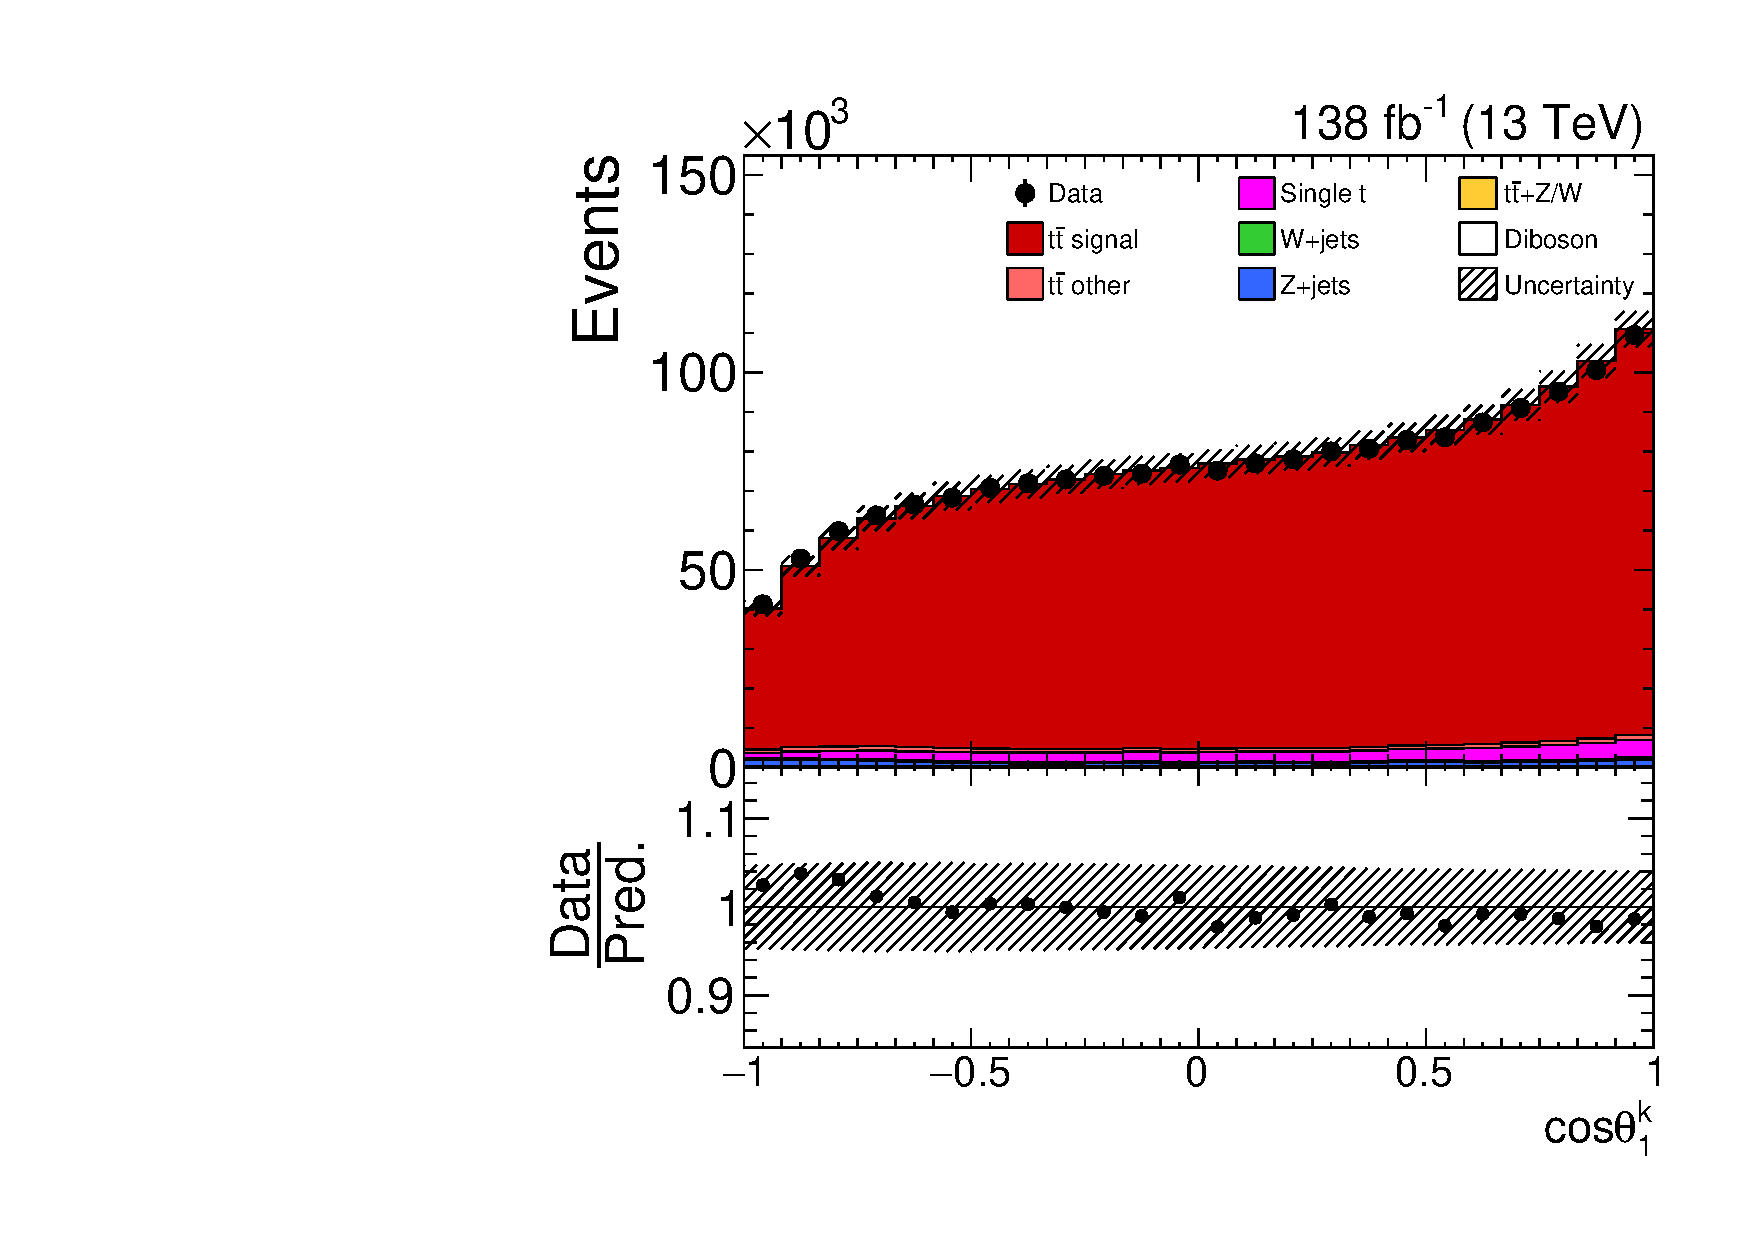
\includegraphics[width=0.32\textwidth]{fig_fullRun2UL/controlplots/combined/Hyp_AntiLeptonBk.pdf}
 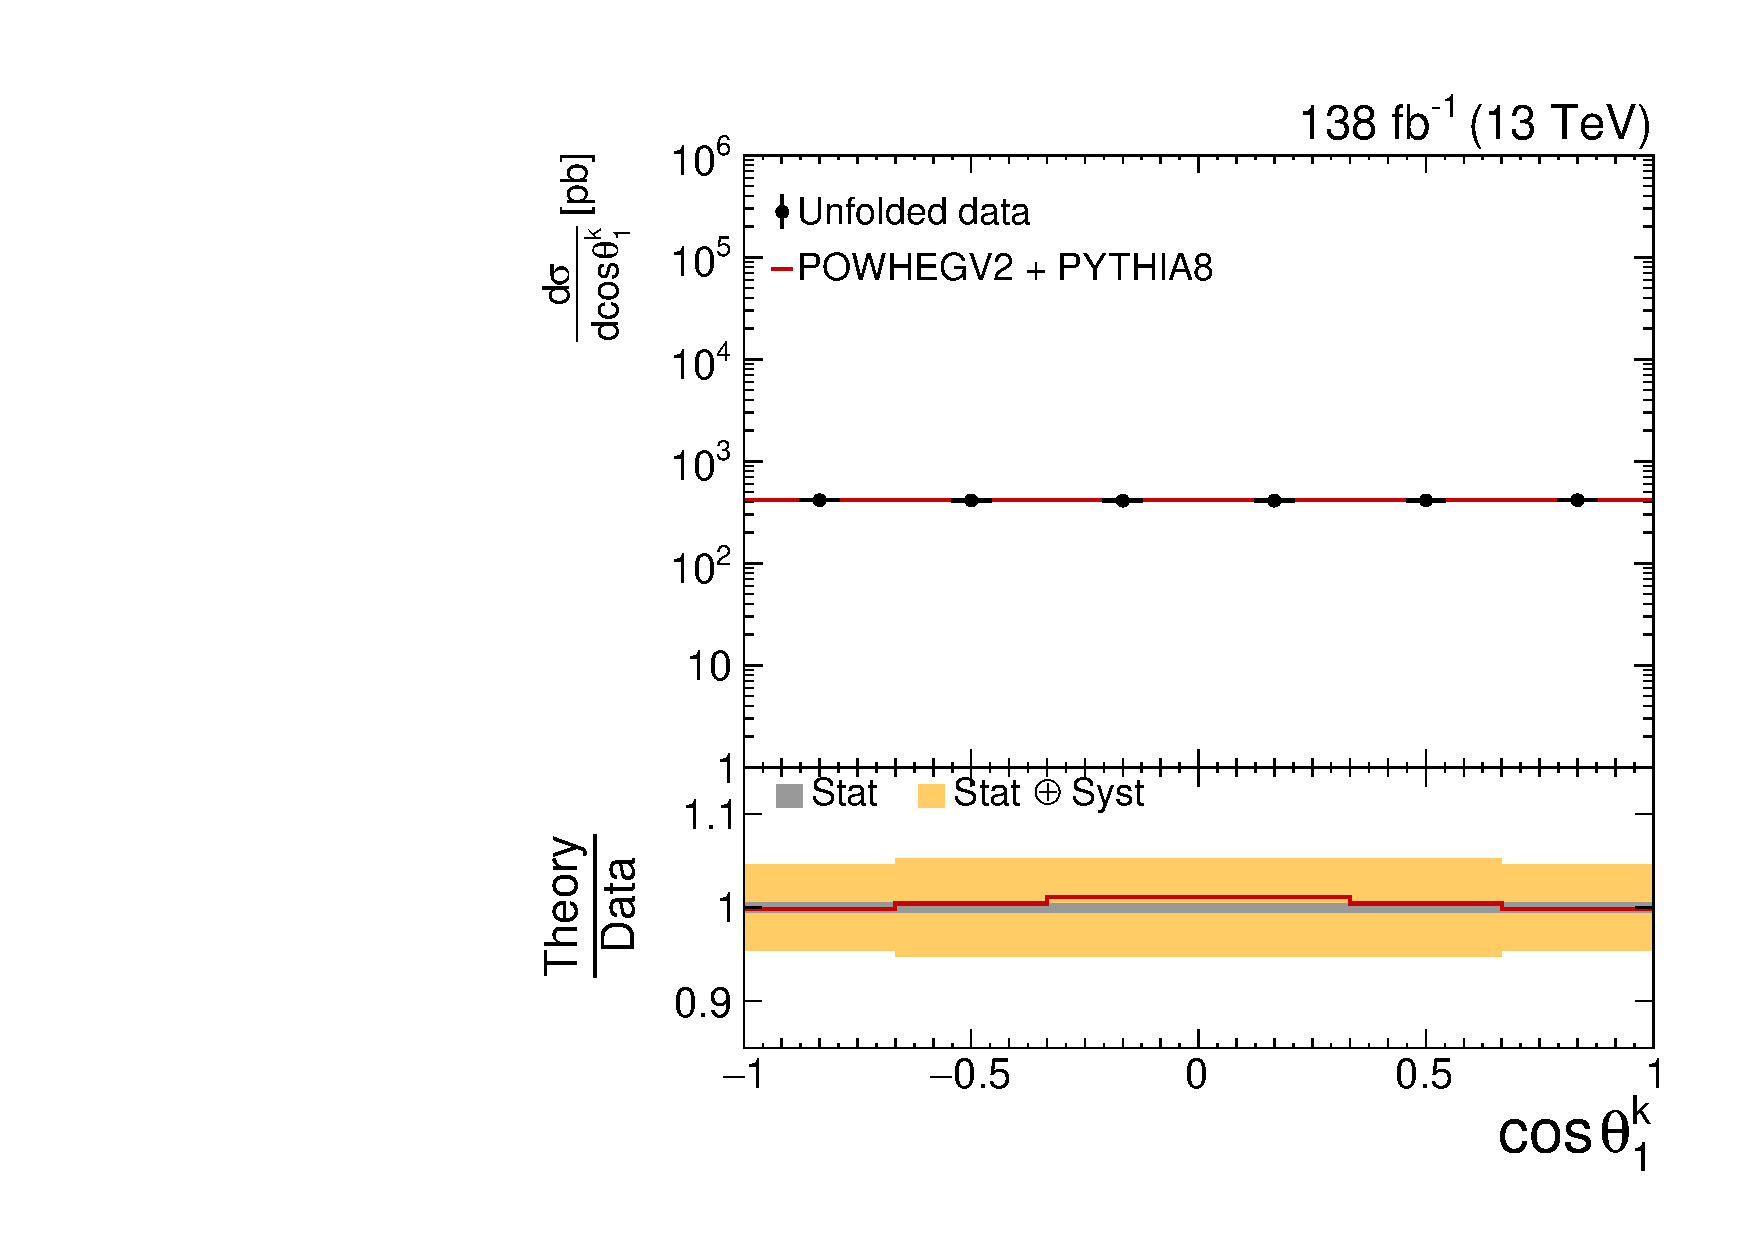
\includegraphics[width=0.32\textwidth]{fig_fullRun2UL/unfolding/combined/UnfoldedResults_b1k.pdf}
 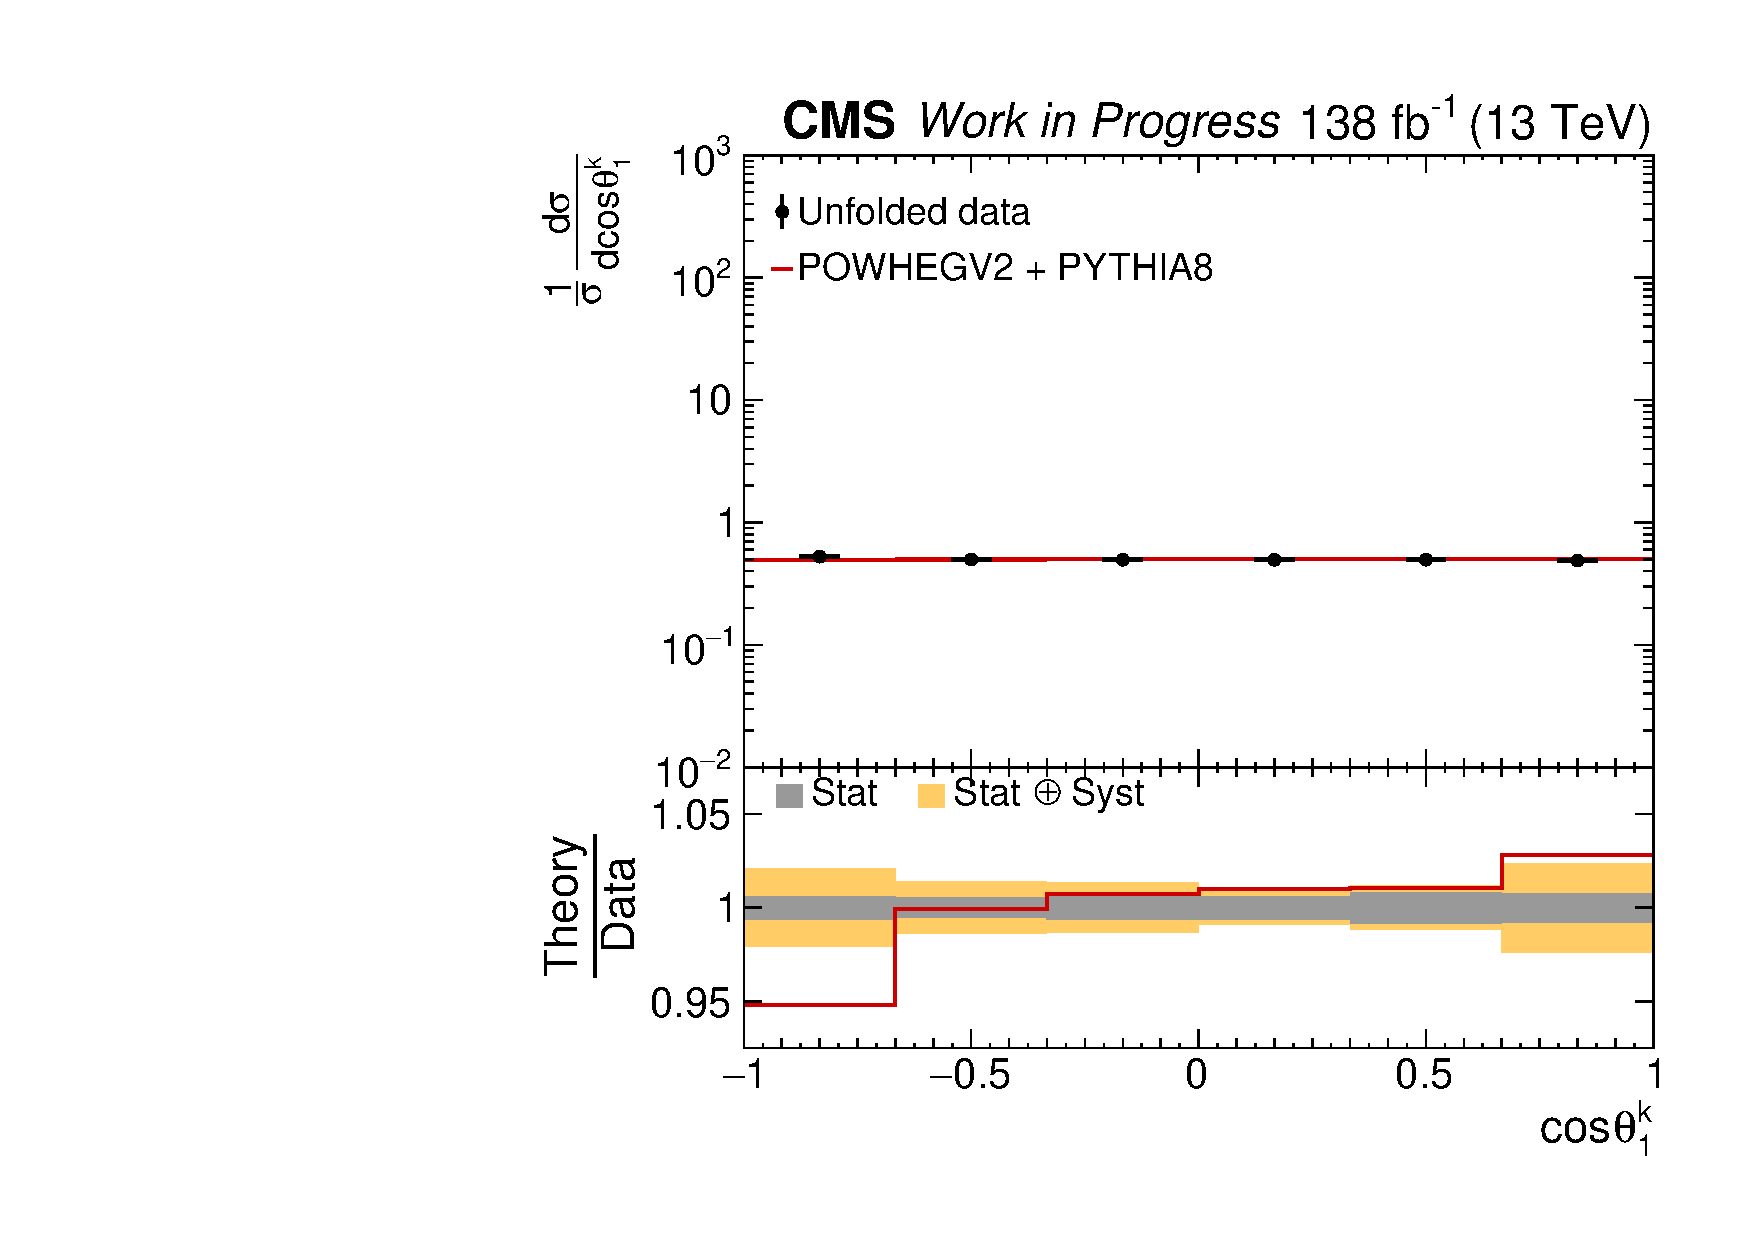
\includegraphics[width=0.32\textwidth]{fig_fullRun2UL/unfolding/combined/UnfoldedResultsNorm_b1k.pdf} \\
 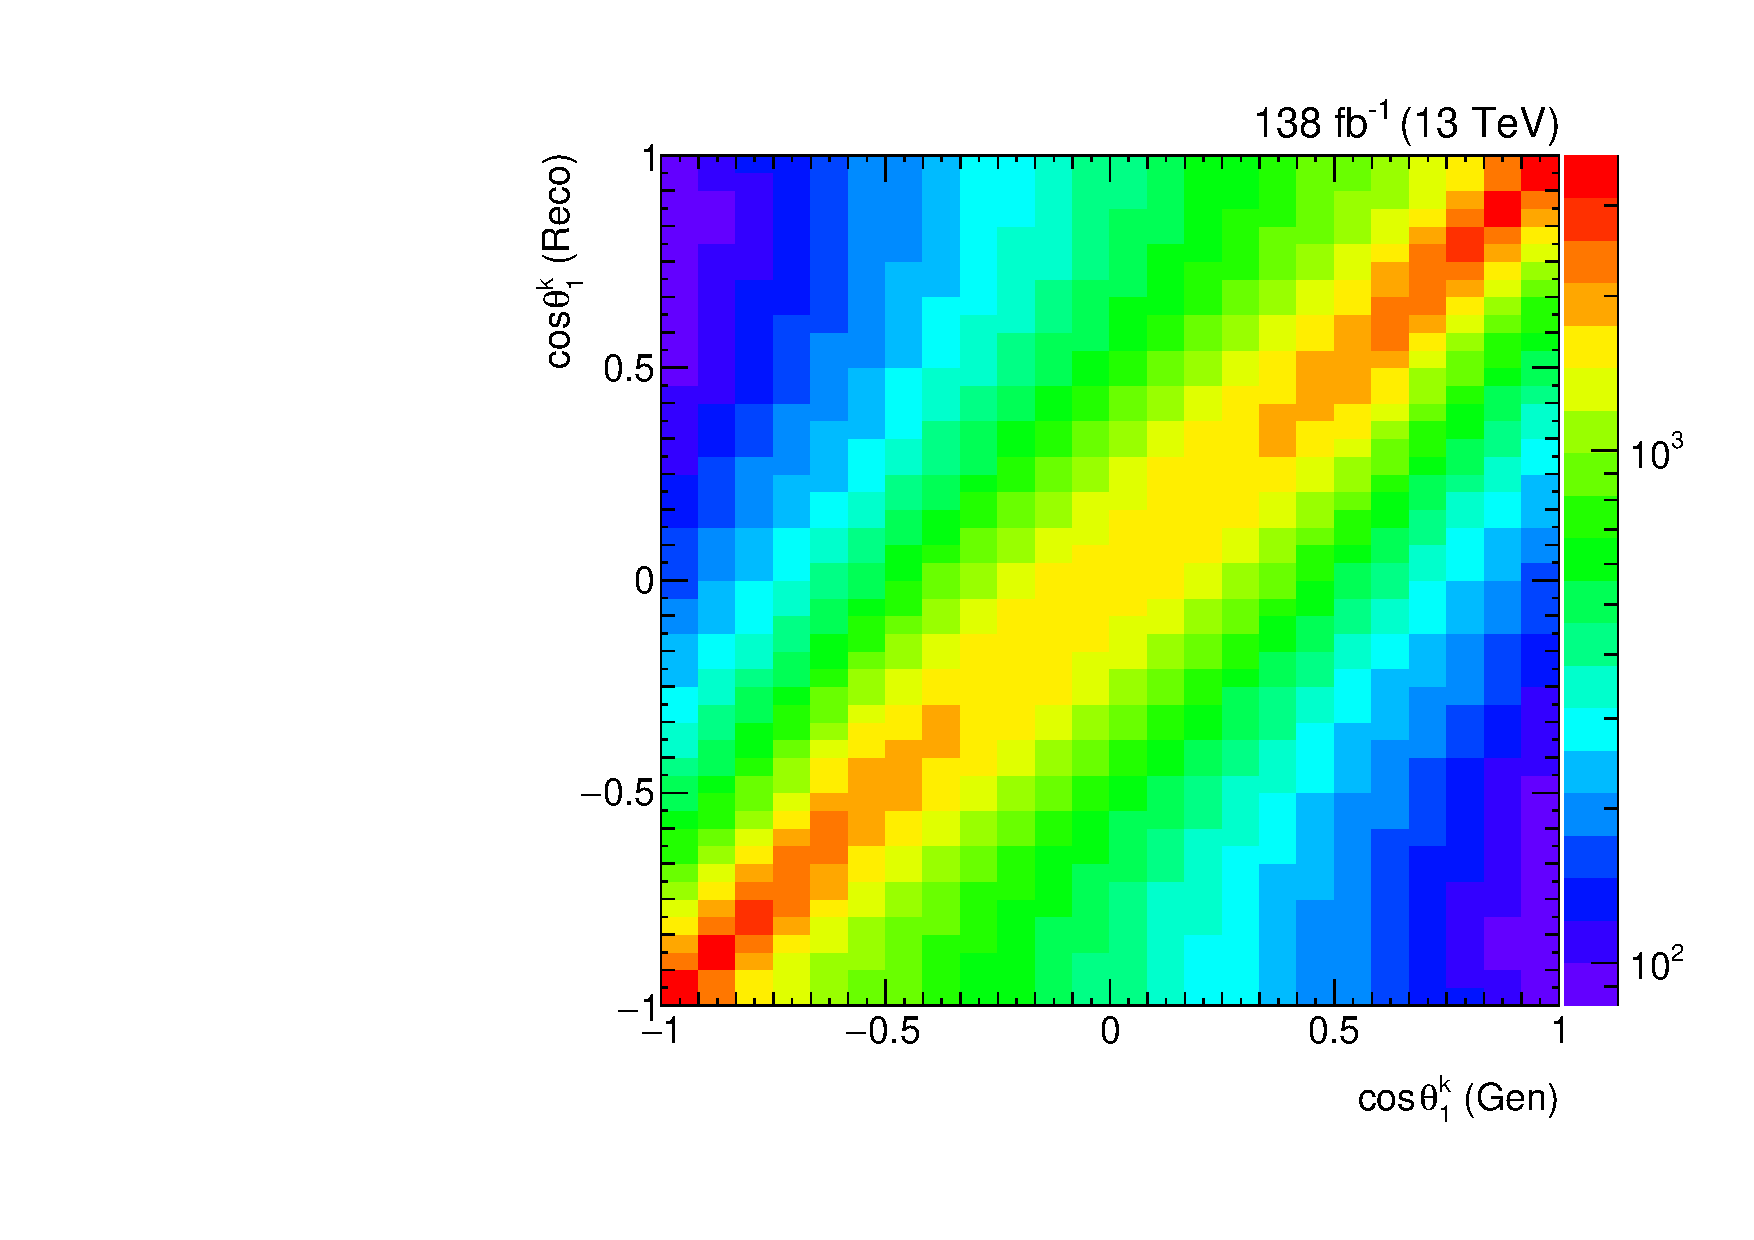
\includegraphics[width=0.32\textwidth]{fig_fullRun2UL/unfolding/combined/ResponseMatrix_b1k.pdf}
 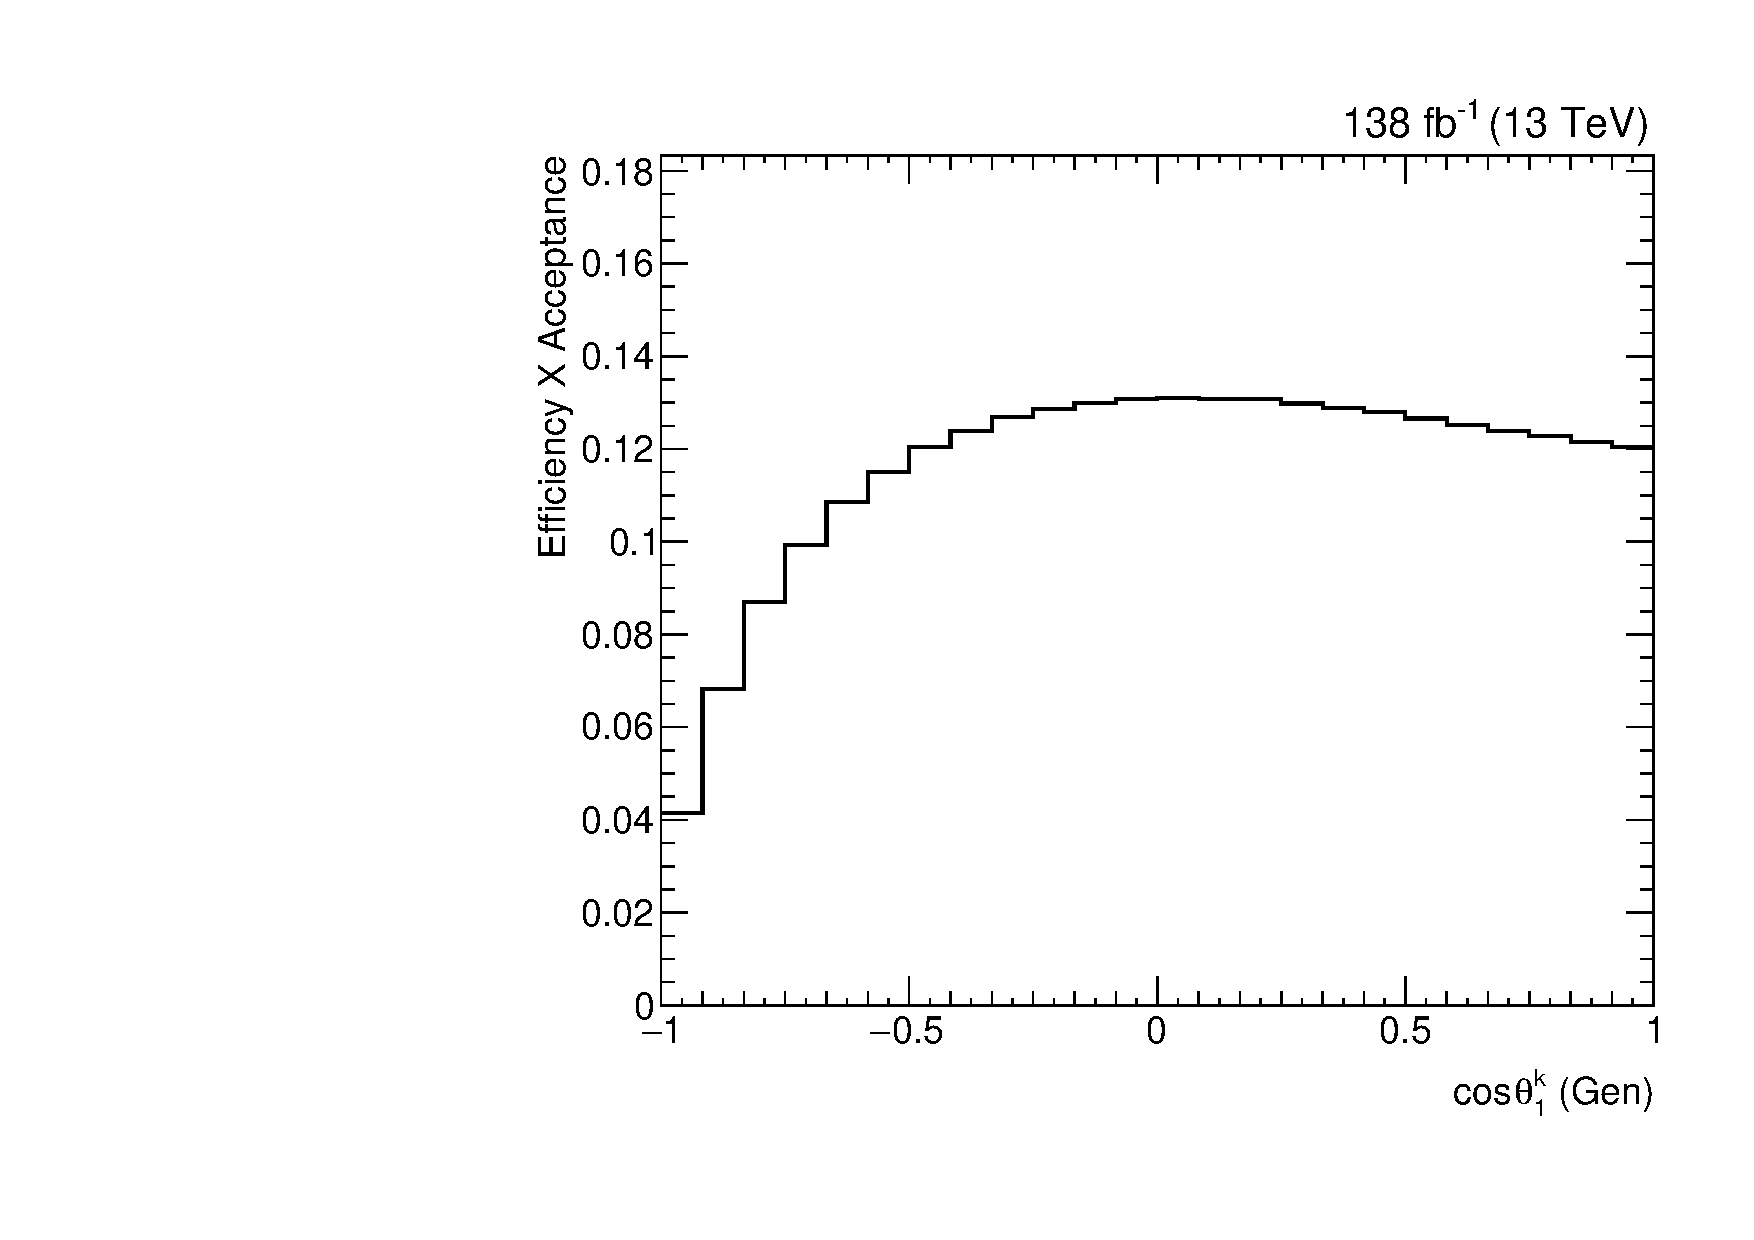
\includegraphics[width=0.32\textwidth]{fig_fullRun2UL/unfolding/combined/TotEff_b1k.pdf}
 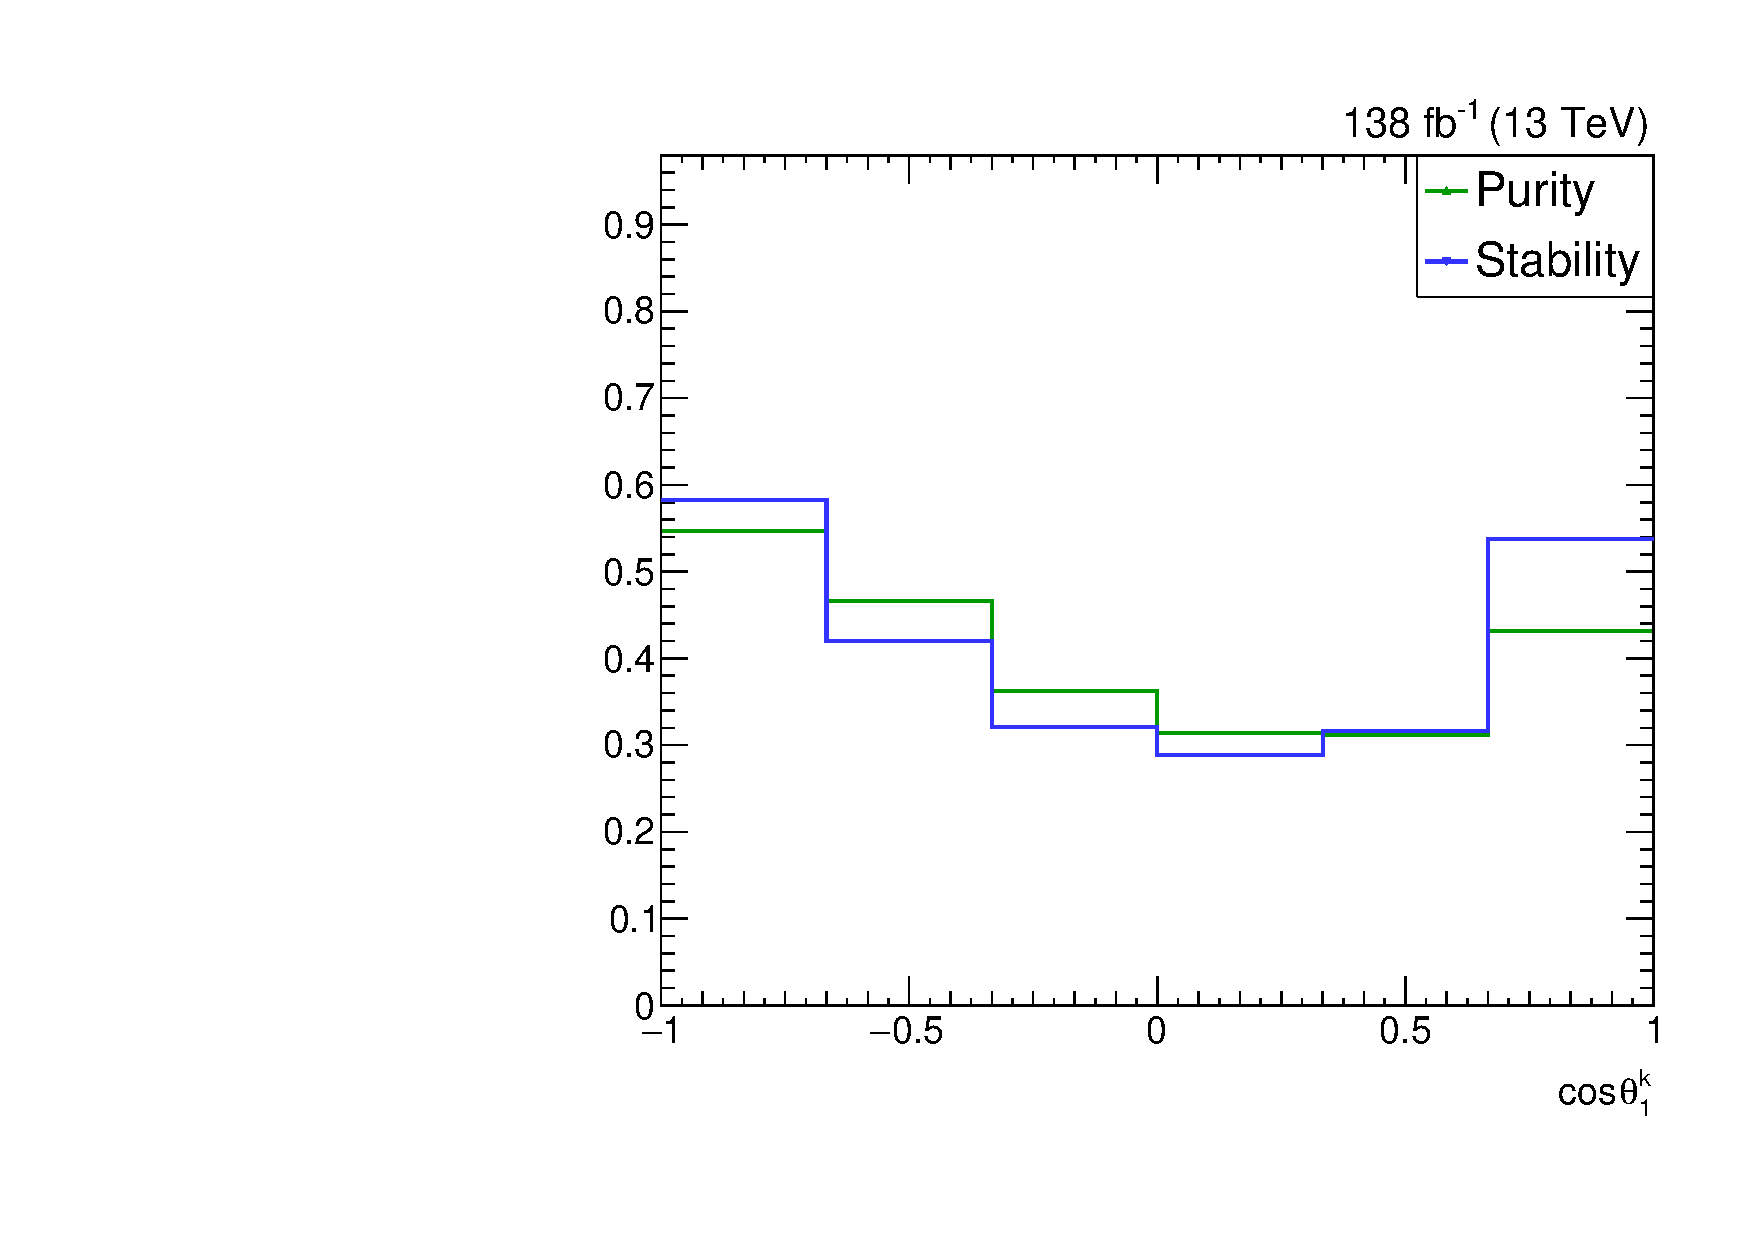
\includegraphics[width=0.32\textwidth]{fig_fullRun2UL/unfolding/combined/PurStab_b1k.pdf} \\
\caption{Reconstructed detector-level distribution (Top Left), absolute cross-section unfolded to parton-level (Top Middle), normalized cross-section unfolded to parton-level (Top Right), detector response-matrix (Bottom Left), efficiency$\times$acceptance (Bottom Middle), Purity and Stability (Bottom Right) for polarization observable $\cos\theta_{1}^{k}$, from which spin-density coefficient $B_{1}^{k}$ (sensitive to spin-density coefficient function $b_k^{+}$) is extracted.}
\label{fig:b1k}
\end{center}
\end{figure}
\clearpage
\begin{figure}[htb]
\begin{center}
 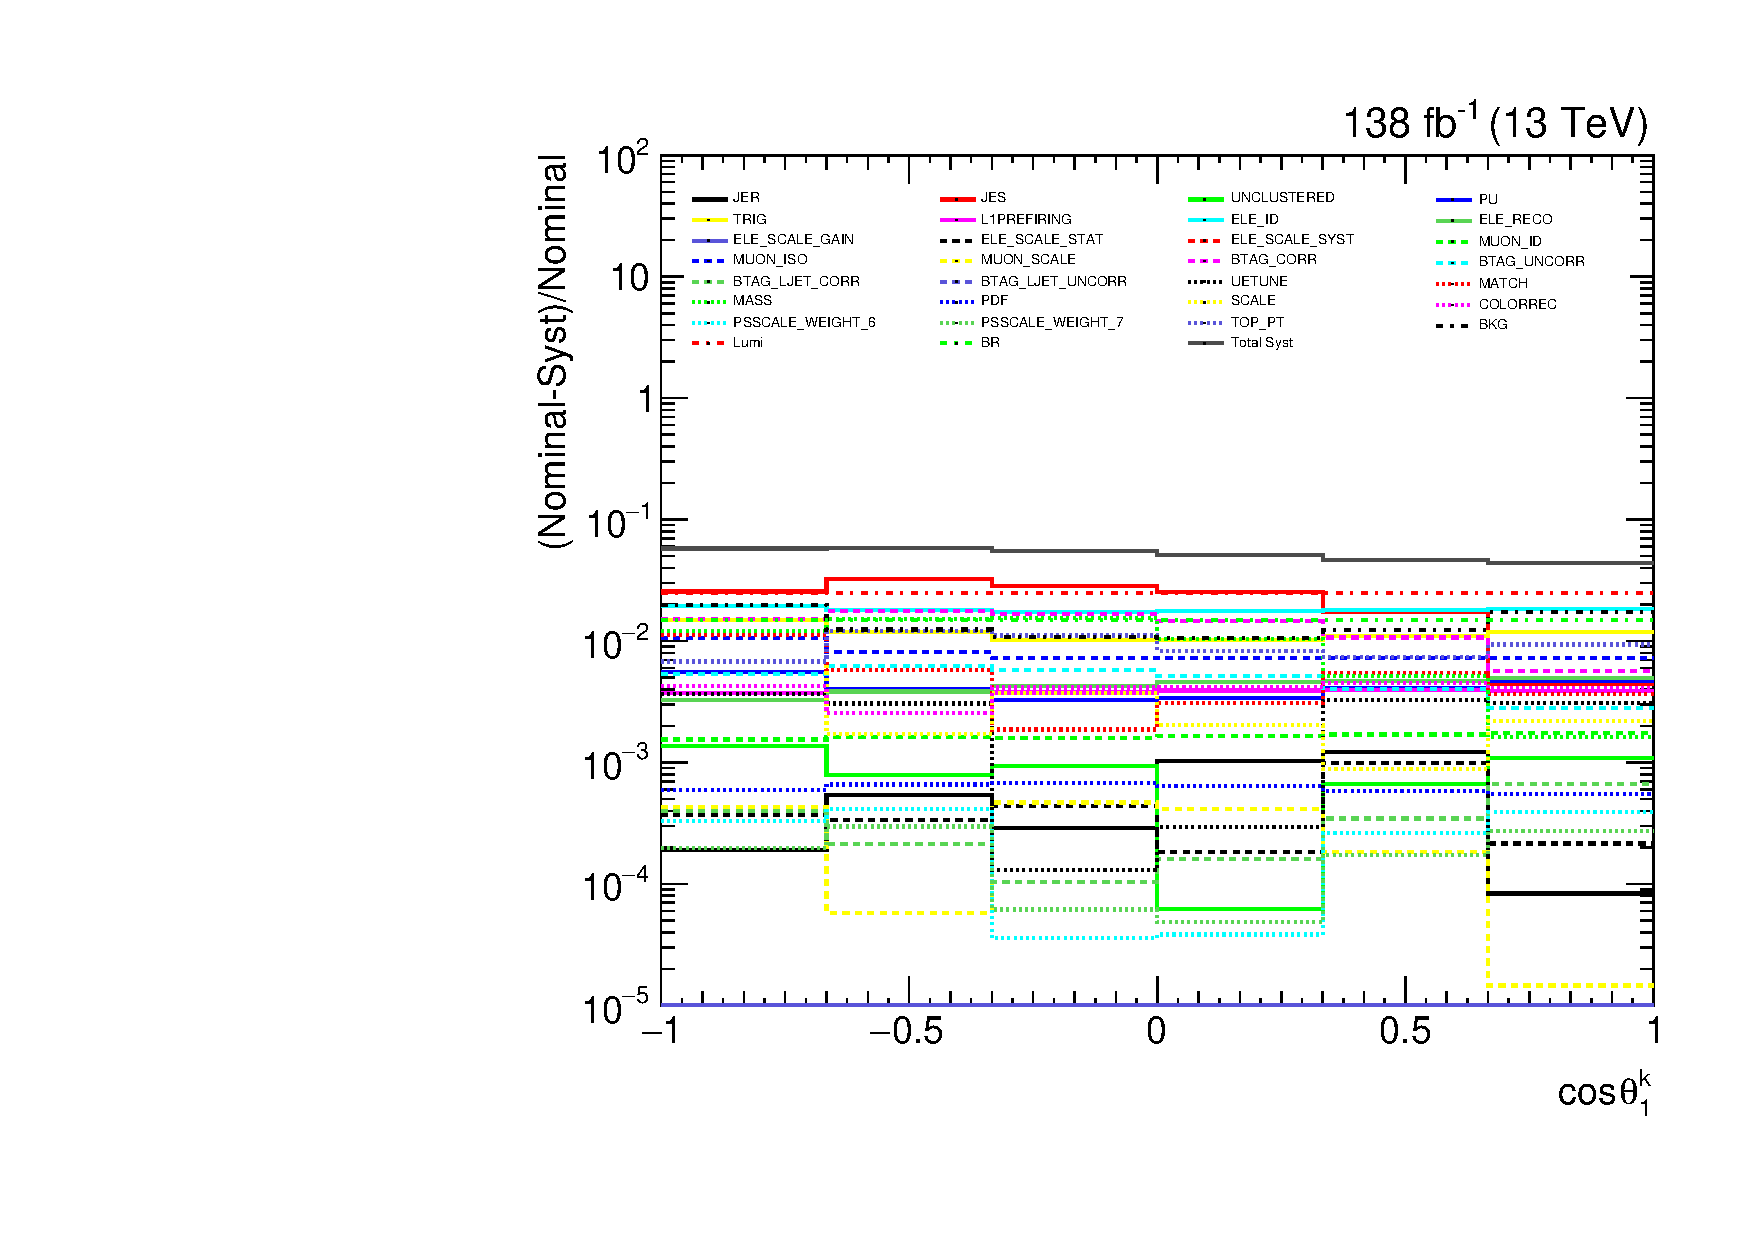
\includegraphics[width=0.32\textwidth]{fig_fullRun2UL/unfolding/combined/deltaSystCombinedlog_rebinnedB_b1k.pdf}
 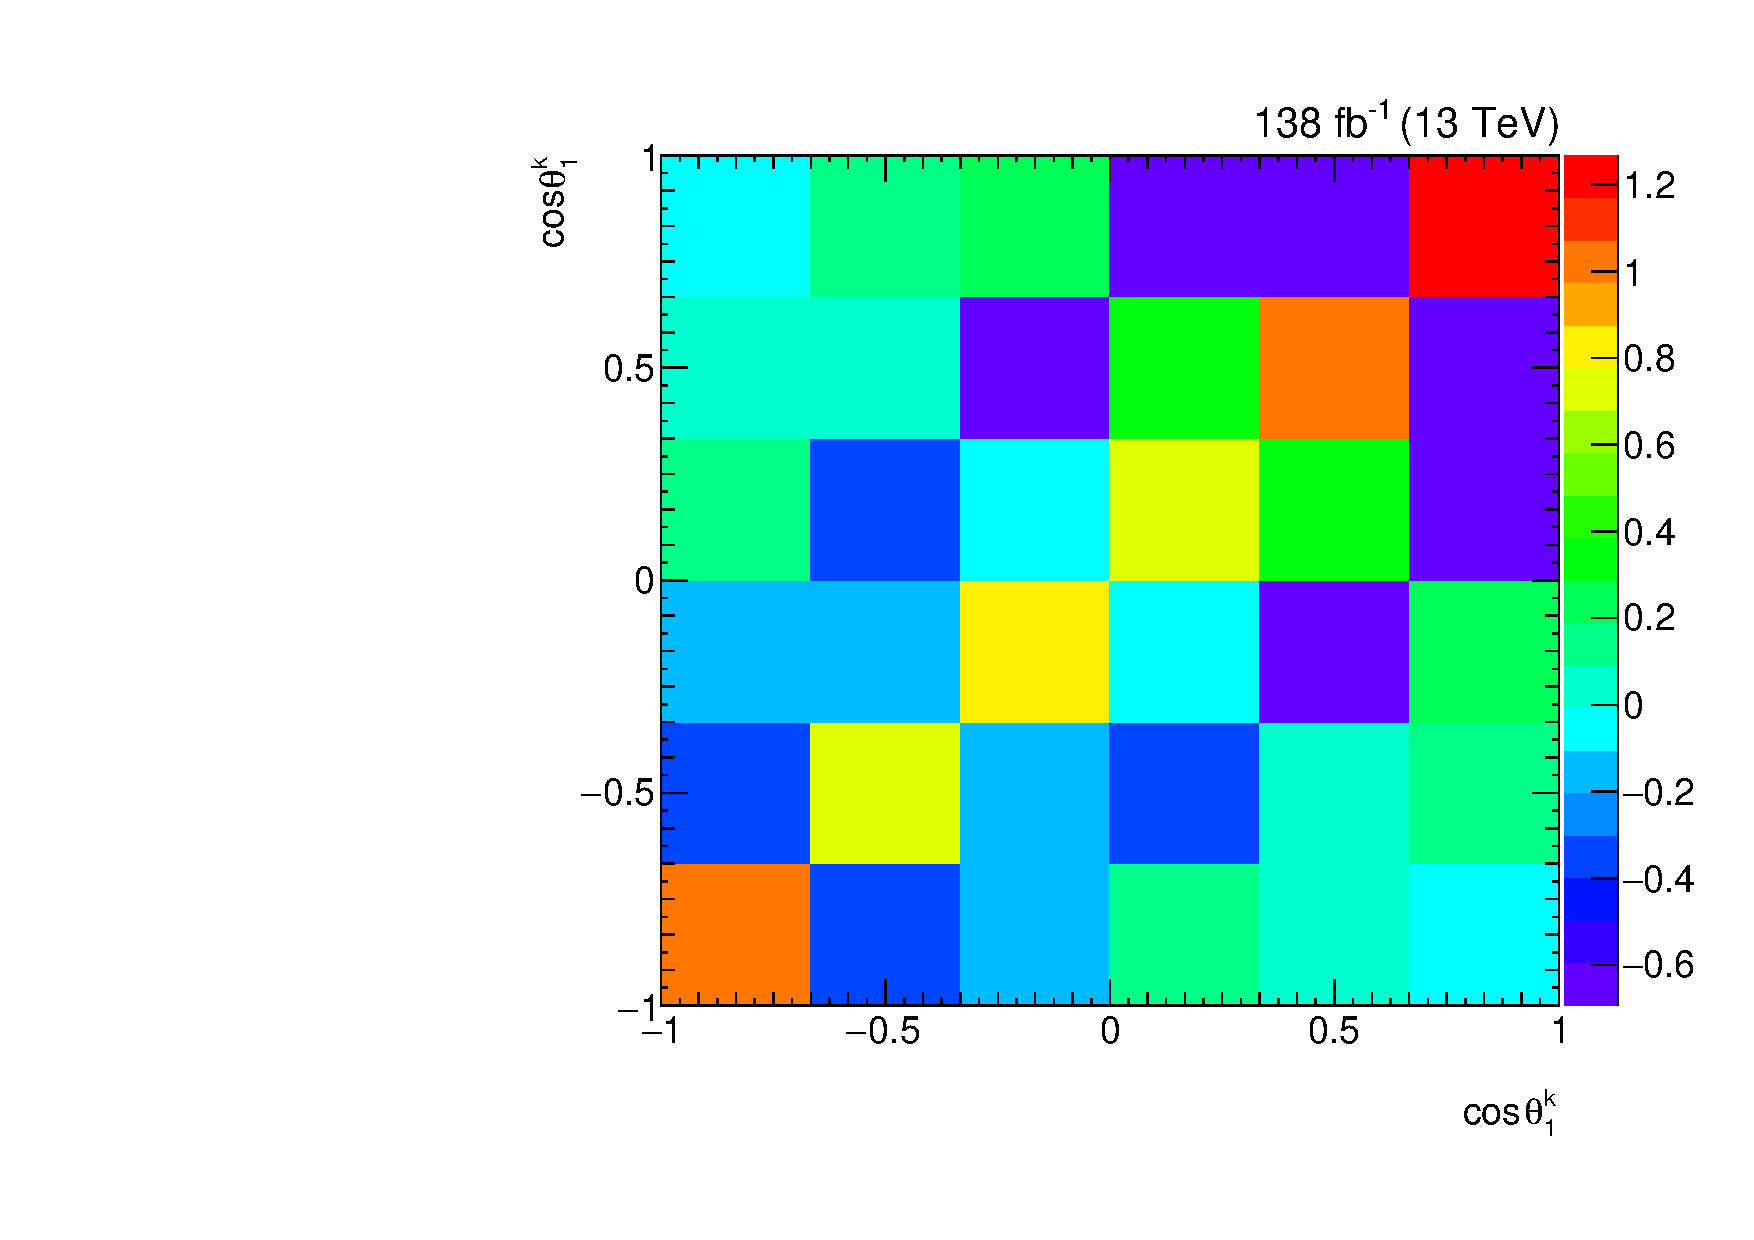
\includegraphics[width=0.32\textwidth]{fig_fullRun2UL/unfolding/combined/StatCovMatrix_rebinnedB_b1k.pdf}
 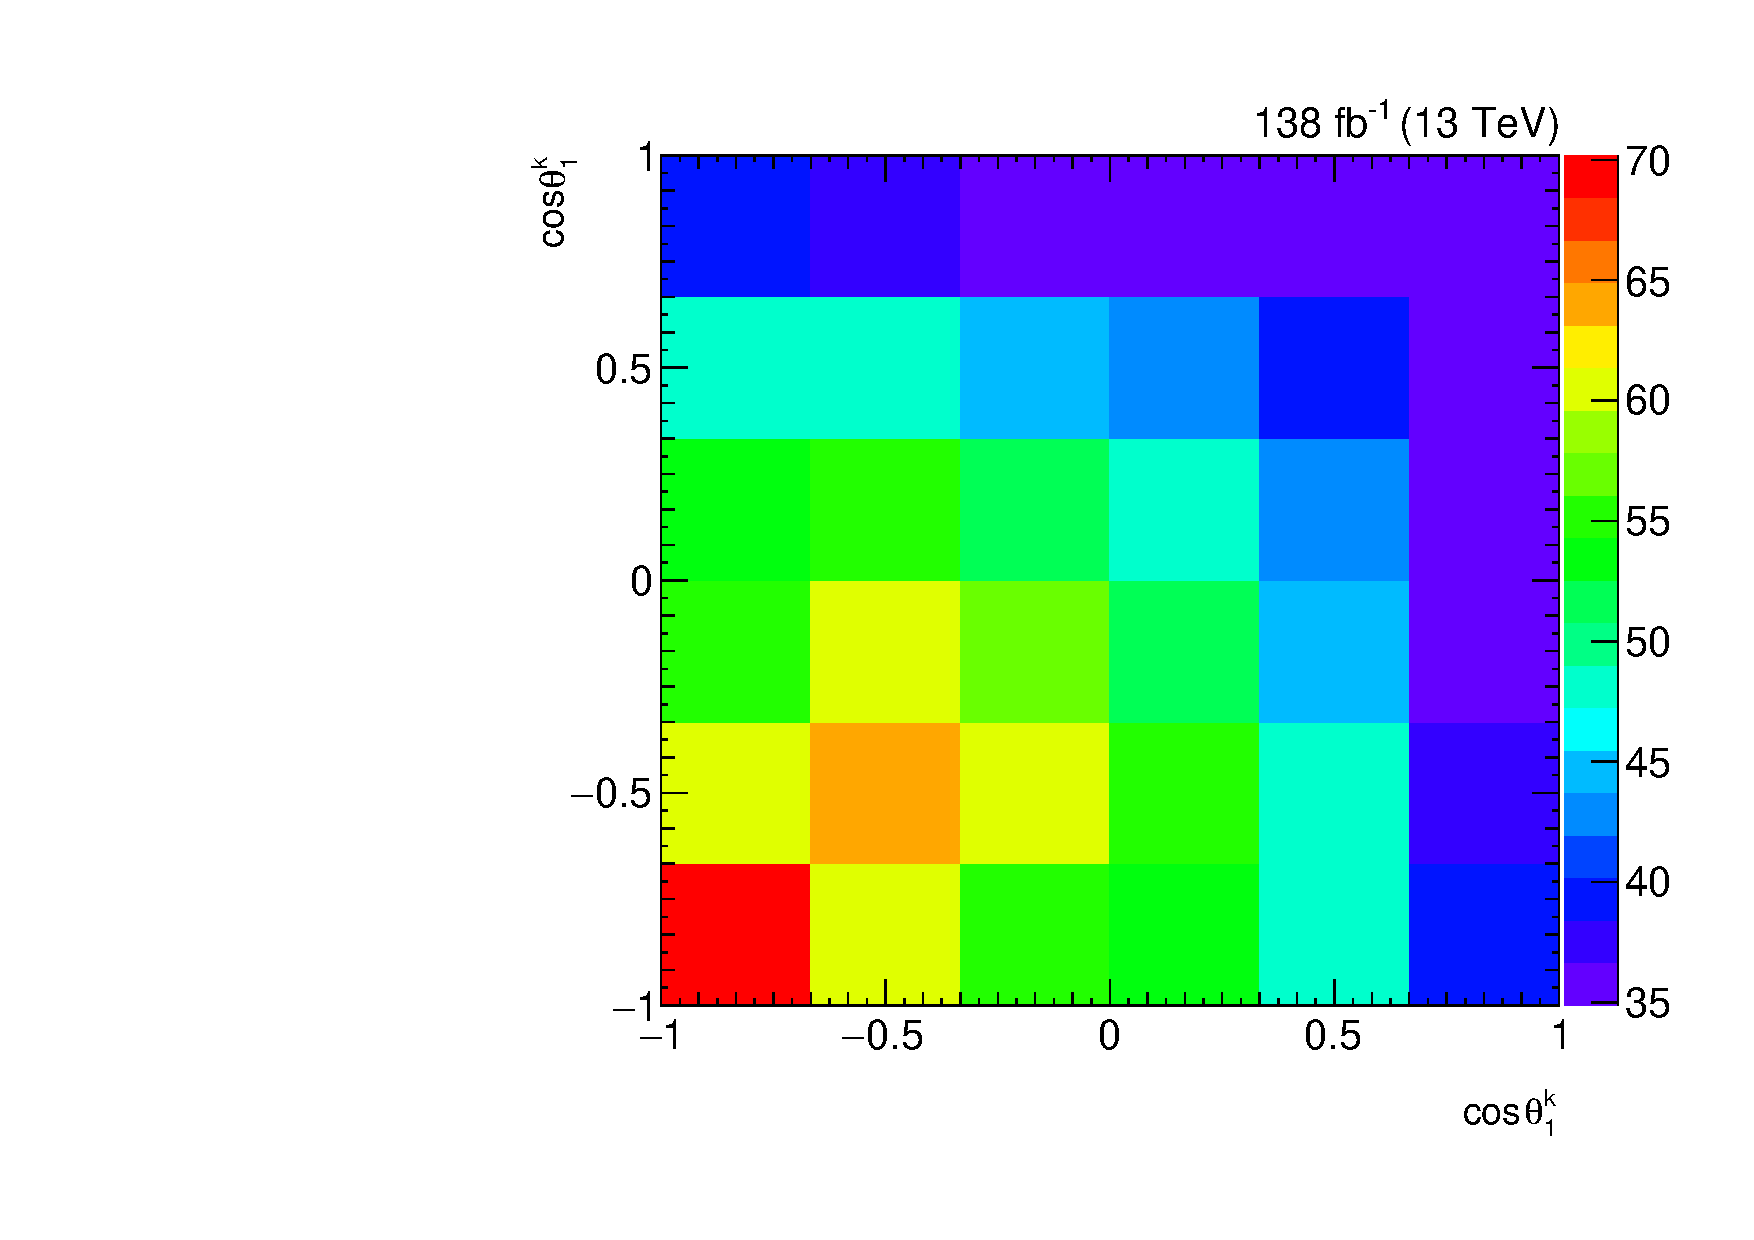
\includegraphics[width=0.32\textwidth]{fig_fullRun2UL/unfolding/combined/TotalSystCovMatrix_rebinnedB_b1k.pdf} \\
 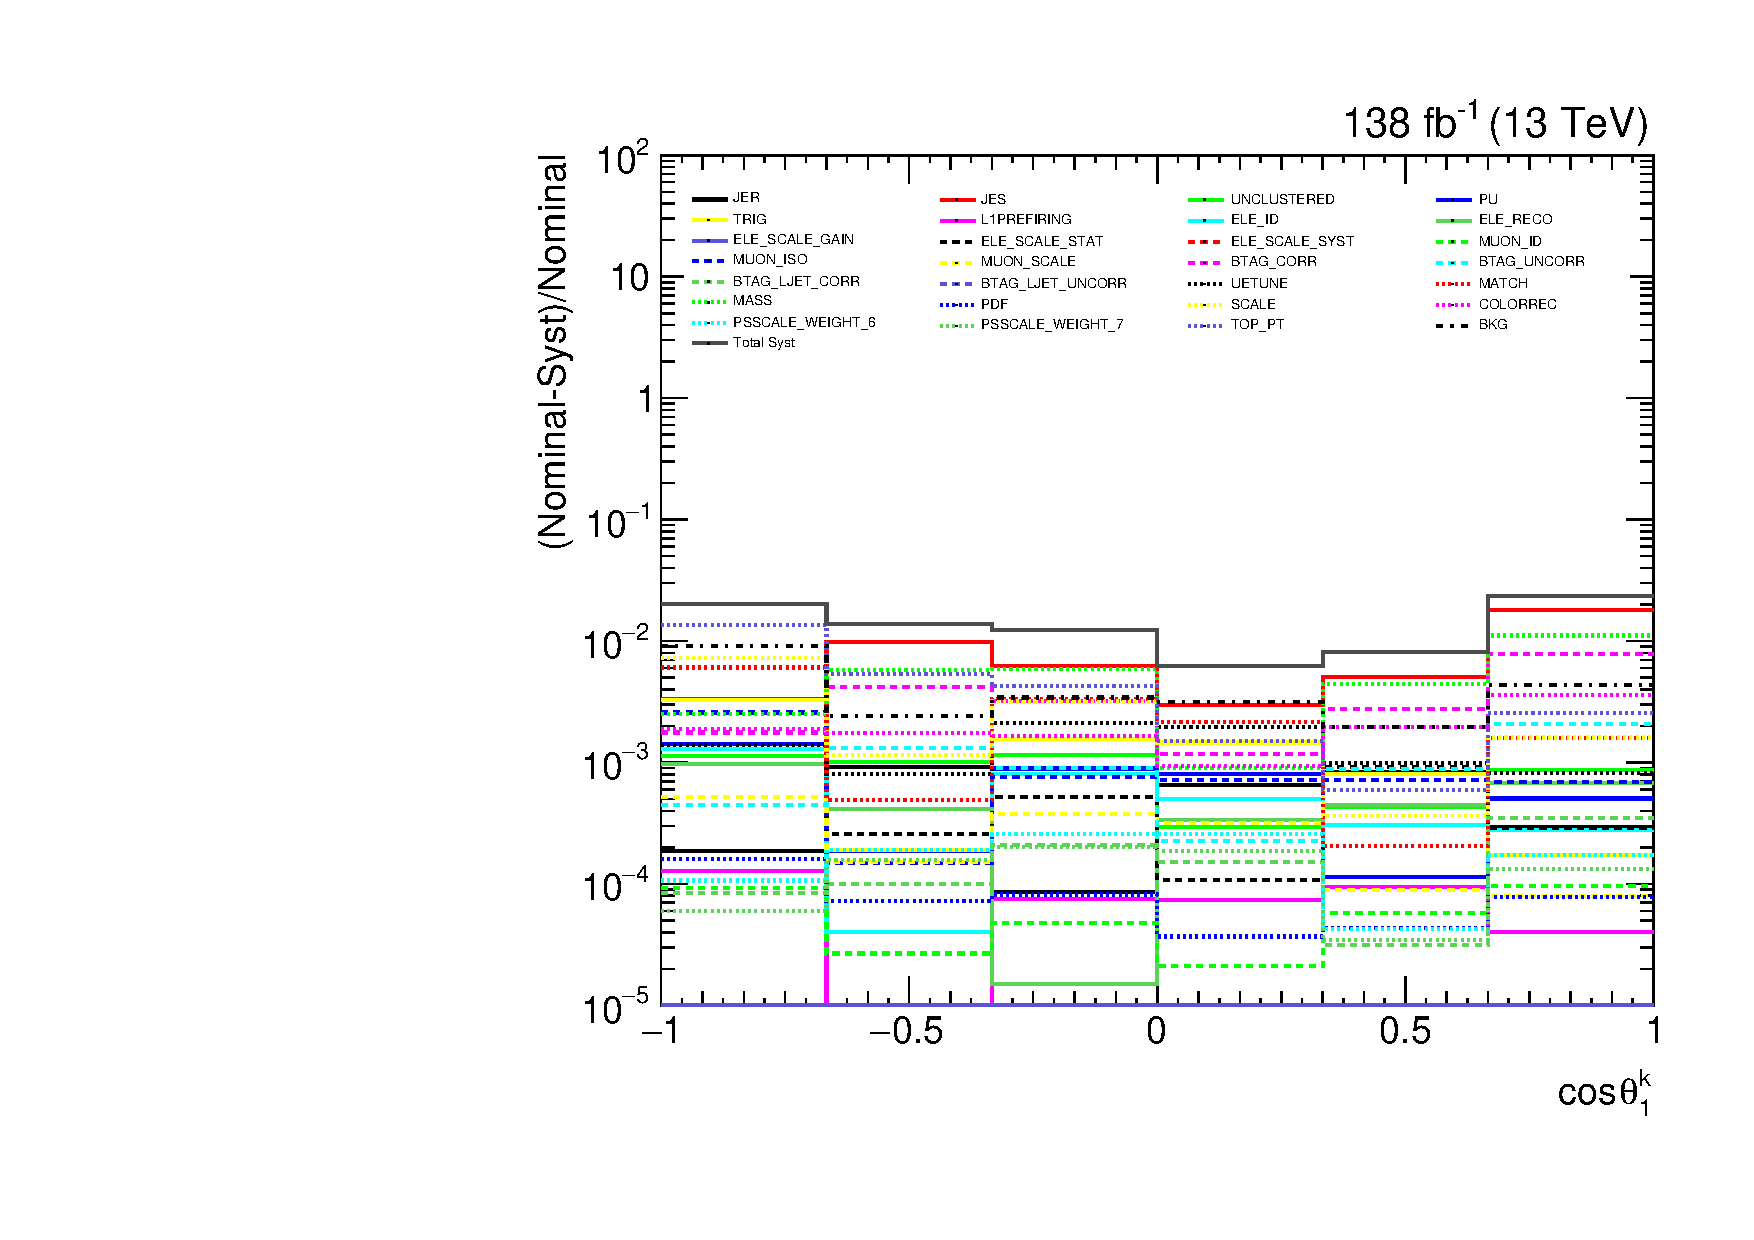
\includegraphics[width=0.32\textwidth]{fig_fullRun2UL/unfolding/combined/deltaSystCombinedlogNorm_rebinnedB_b1k.pdf}
 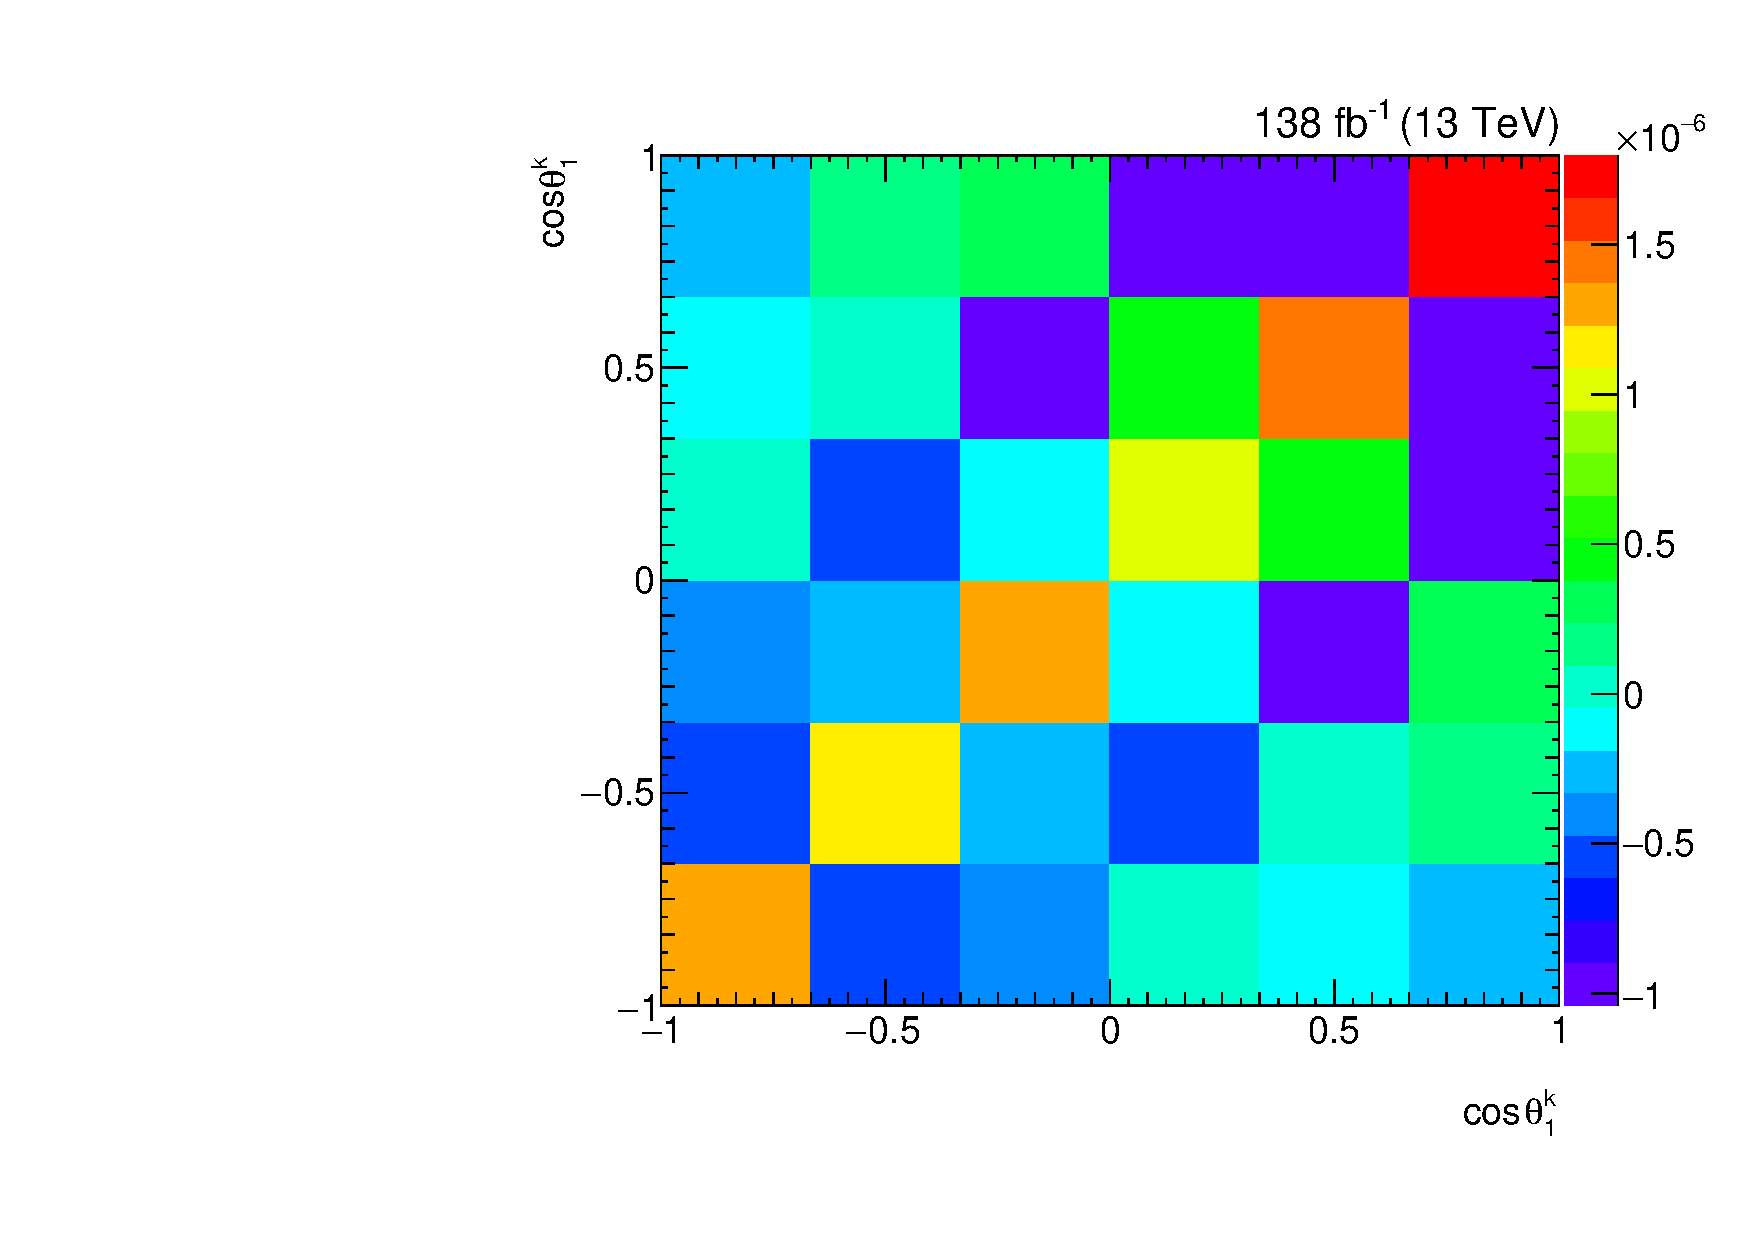
\includegraphics[width=0.32\textwidth]{fig_fullRun2UL/unfolding/combined/StatCovMatrixNorm_rebinnedB_b1k.pdf}
 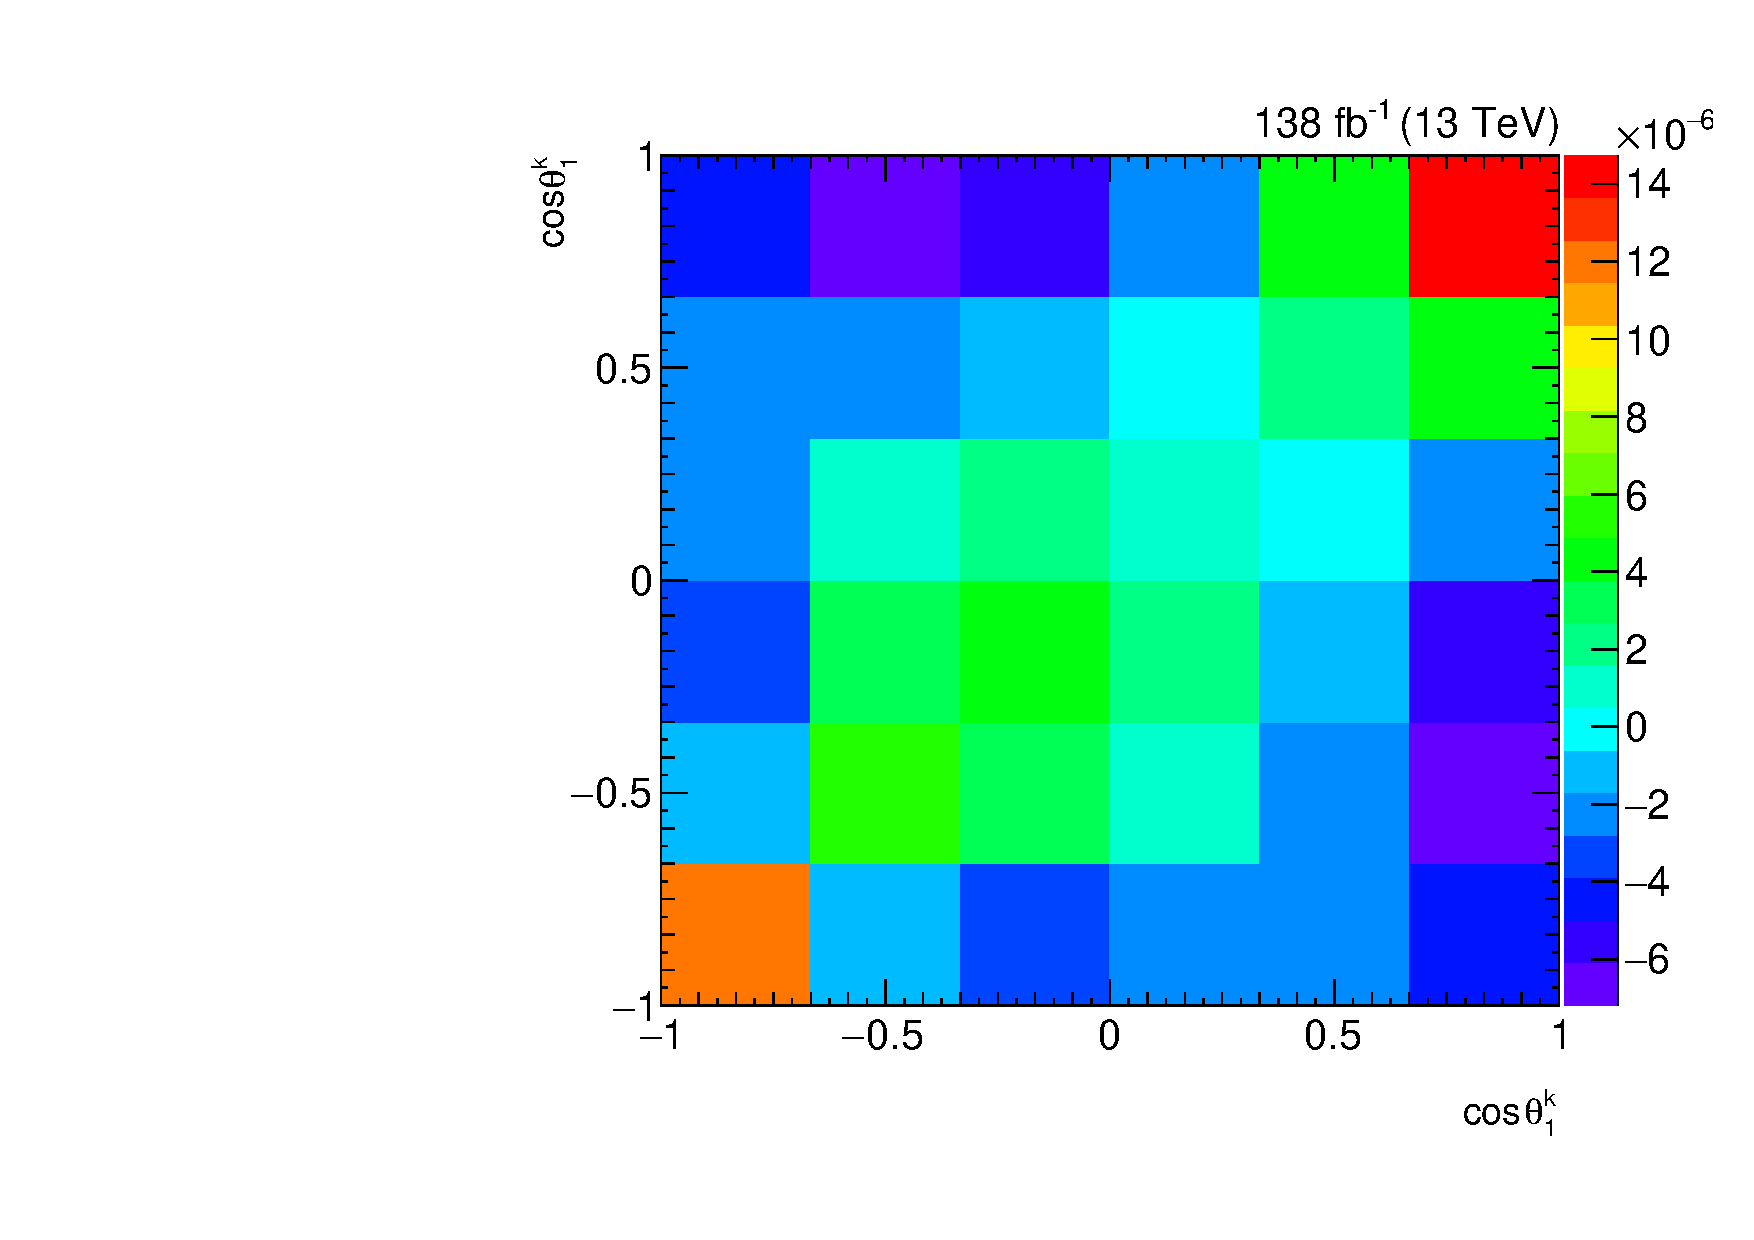
\includegraphics[width=0.32\textwidth]{fig_fullRun2UL/unfolding/combined/TotalSystCovMatrixNorm_rebinnedB_b1k.pdf} \\
\caption{Unfolded-cross section breakdown of uncertainties (Top Left), unfolded cross-section statistical covariance matrix (Top Middle), unfolded cross-section total systematic covariance matrix (Top Right), normalized unfolded-cross section breakdown of uncertainties (Bottom Left), normalized unfolded cross-section statistical covariance matrix (Bottom Middle), normalized unfolded cross-section total systematic covariance matrix (Bottom Right) for polarization observable $\cos\theta_{1}^{k}$.}
\label{fig:b1k_uncertainties}
\end{center}
\end{figure}
\clearpage
\begin{figure}[htb]
\begin{center}
 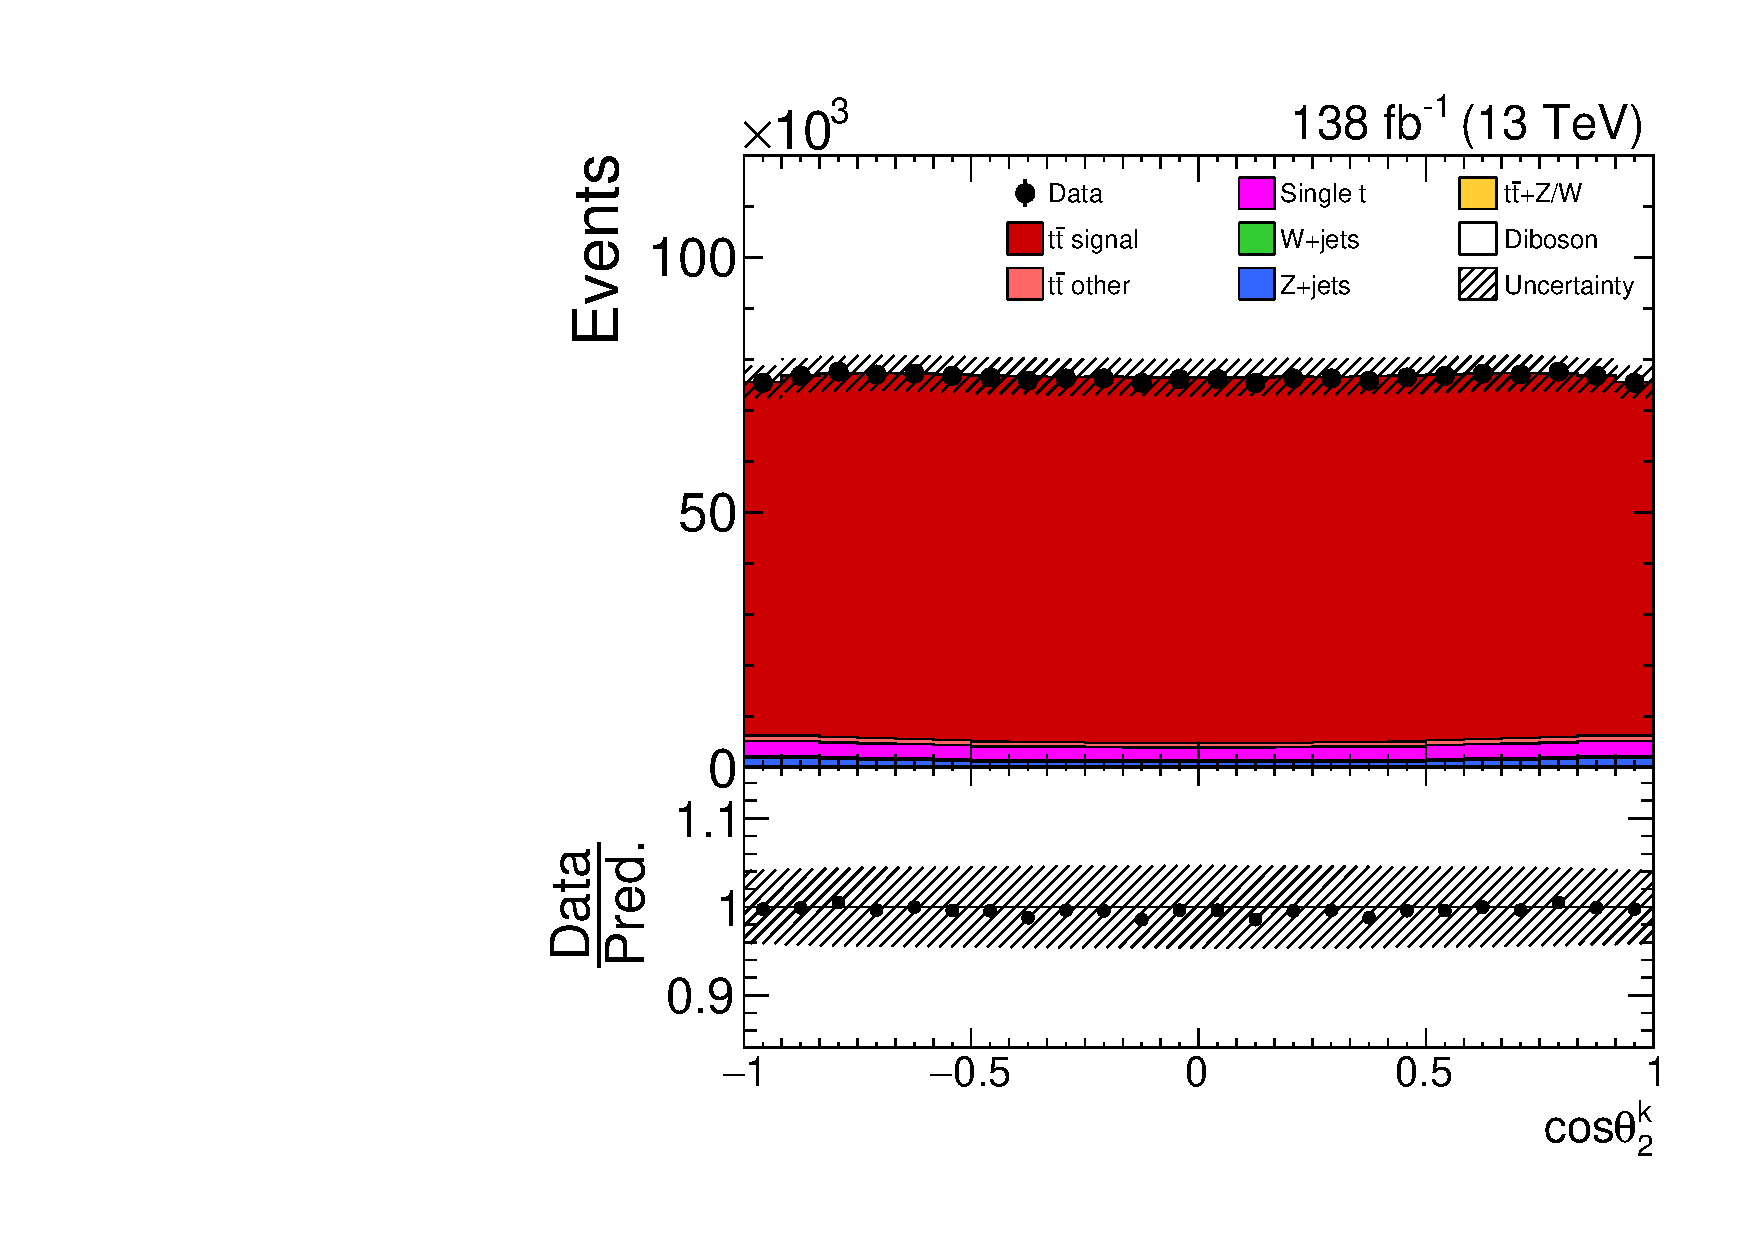
\includegraphics[width=0.32\textwidth]{fig_fullRun2UL/controlplots/combined/Hyp_LeptonBk.pdf}
 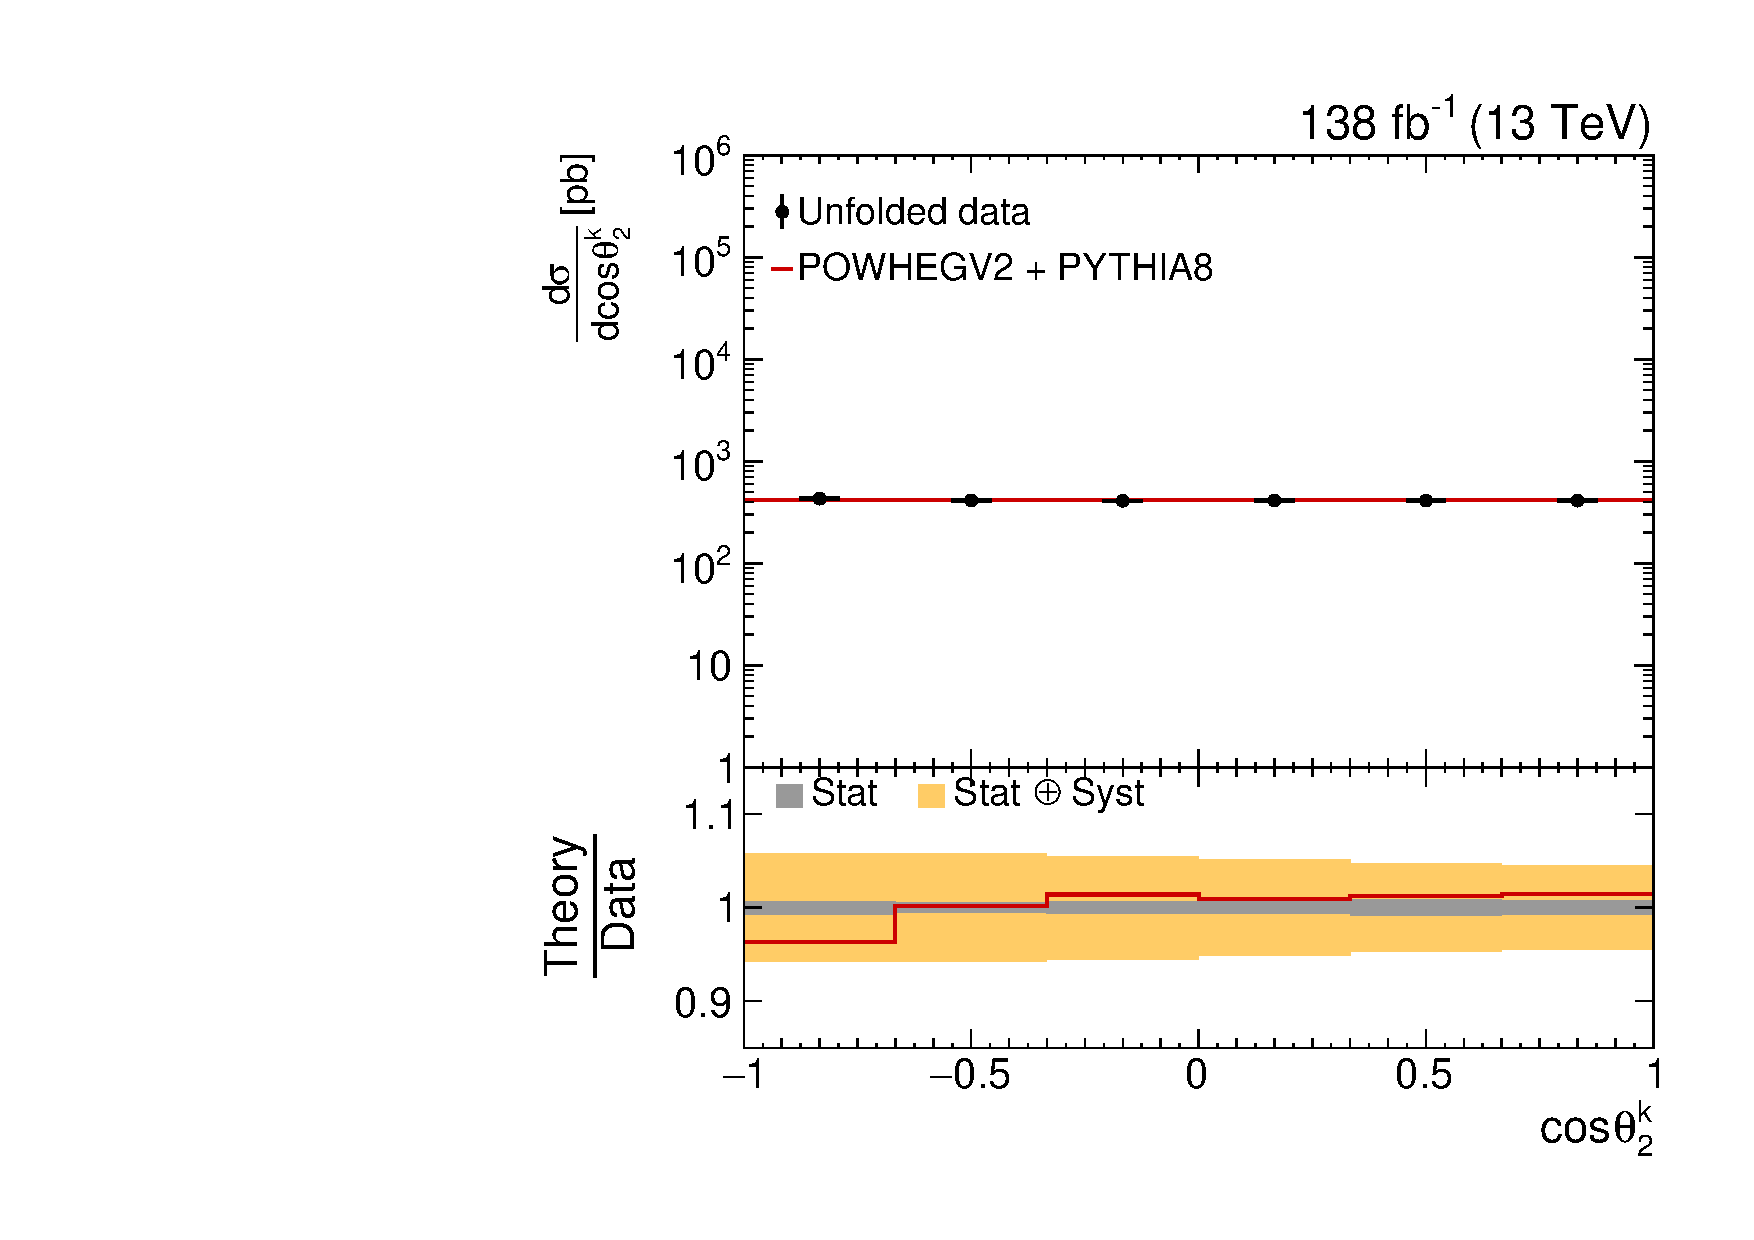
\includegraphics[width=0.32\textwidth]{fig_fullRun2UL/unfolding/combined/UnfoldedResults_b2k.pdf}
 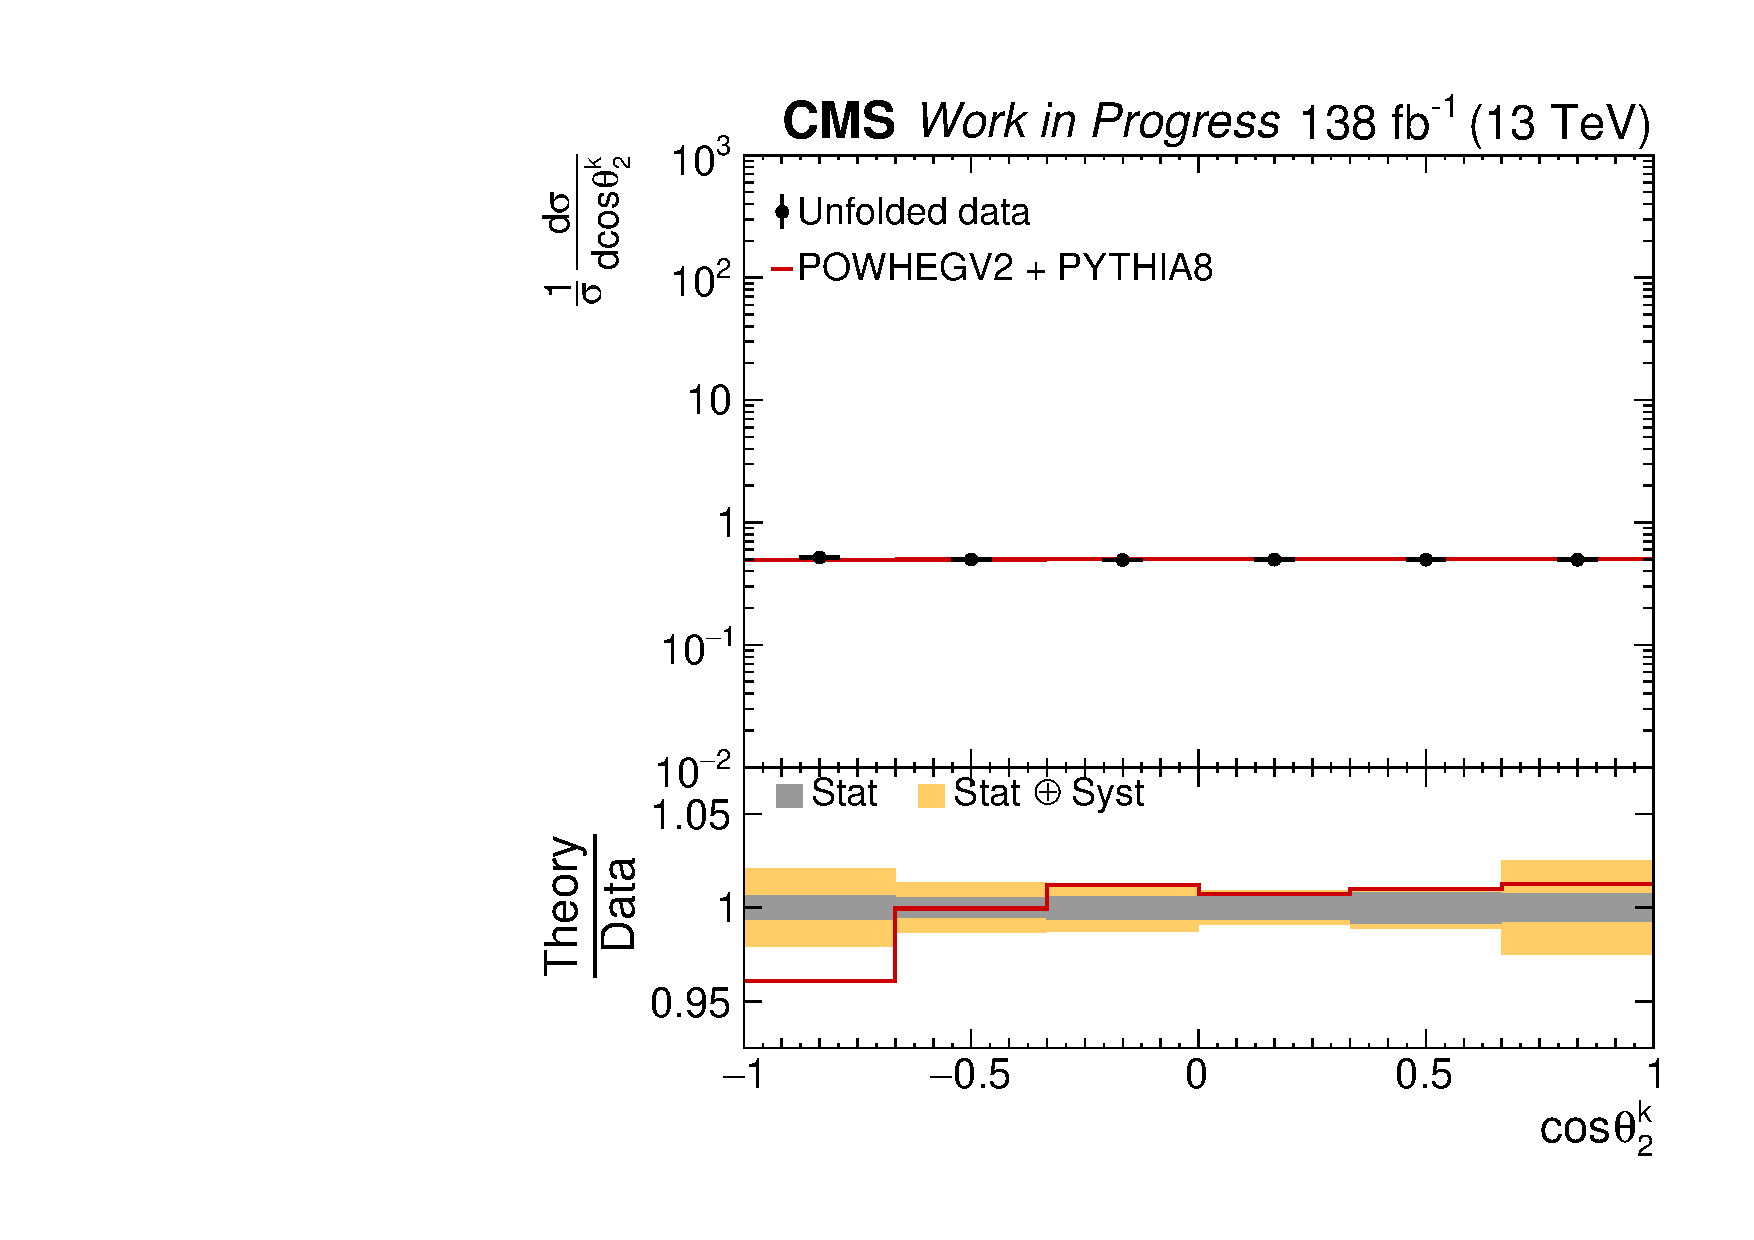
\includegraphics[width=0.32\textwidth]{fig_fullRun2UL/unfolding/combined/UnfoldedResultsNorm_b2k.pdf} \\
 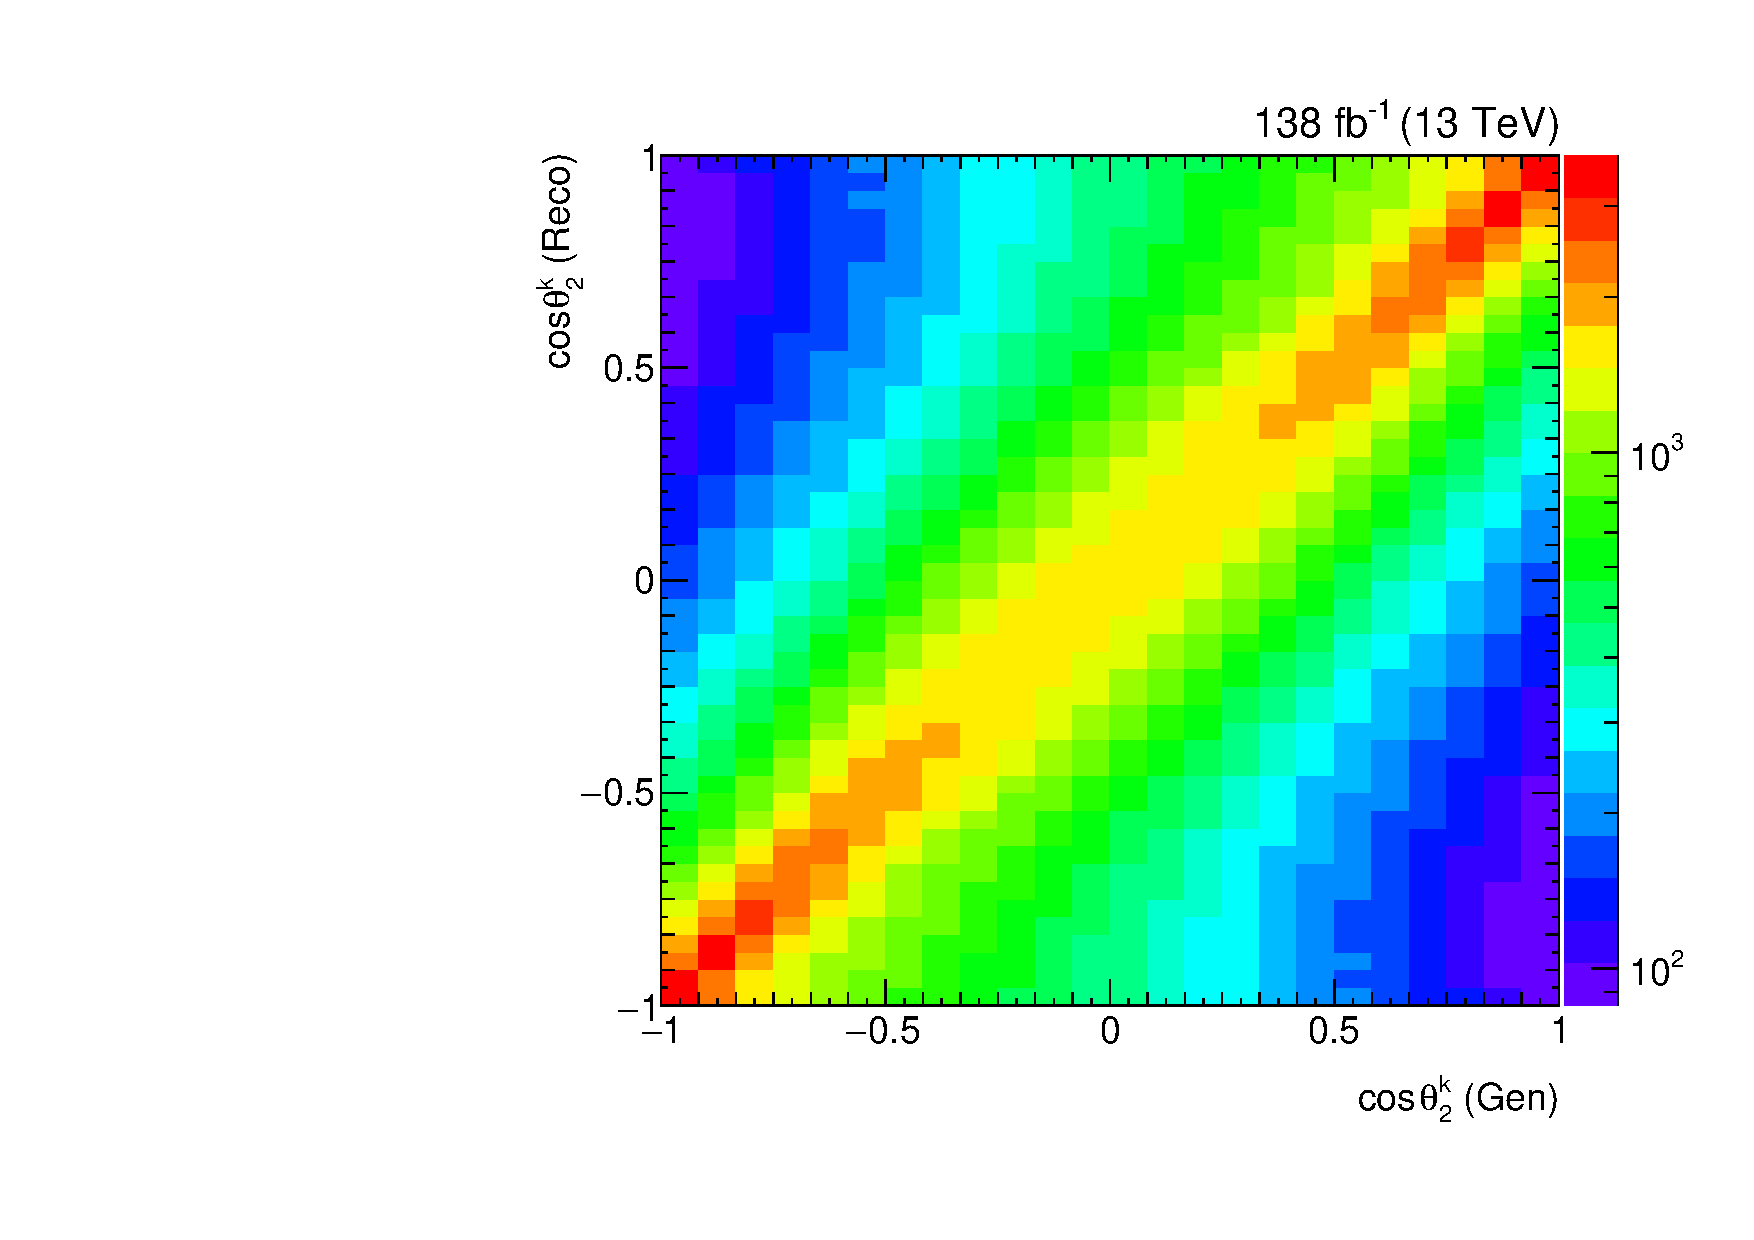
\includegraphics[width=0.32\textwidth]{fig_fullRun2UL/unfolding/combined/ResponseMatrix_b2k.pdf}
 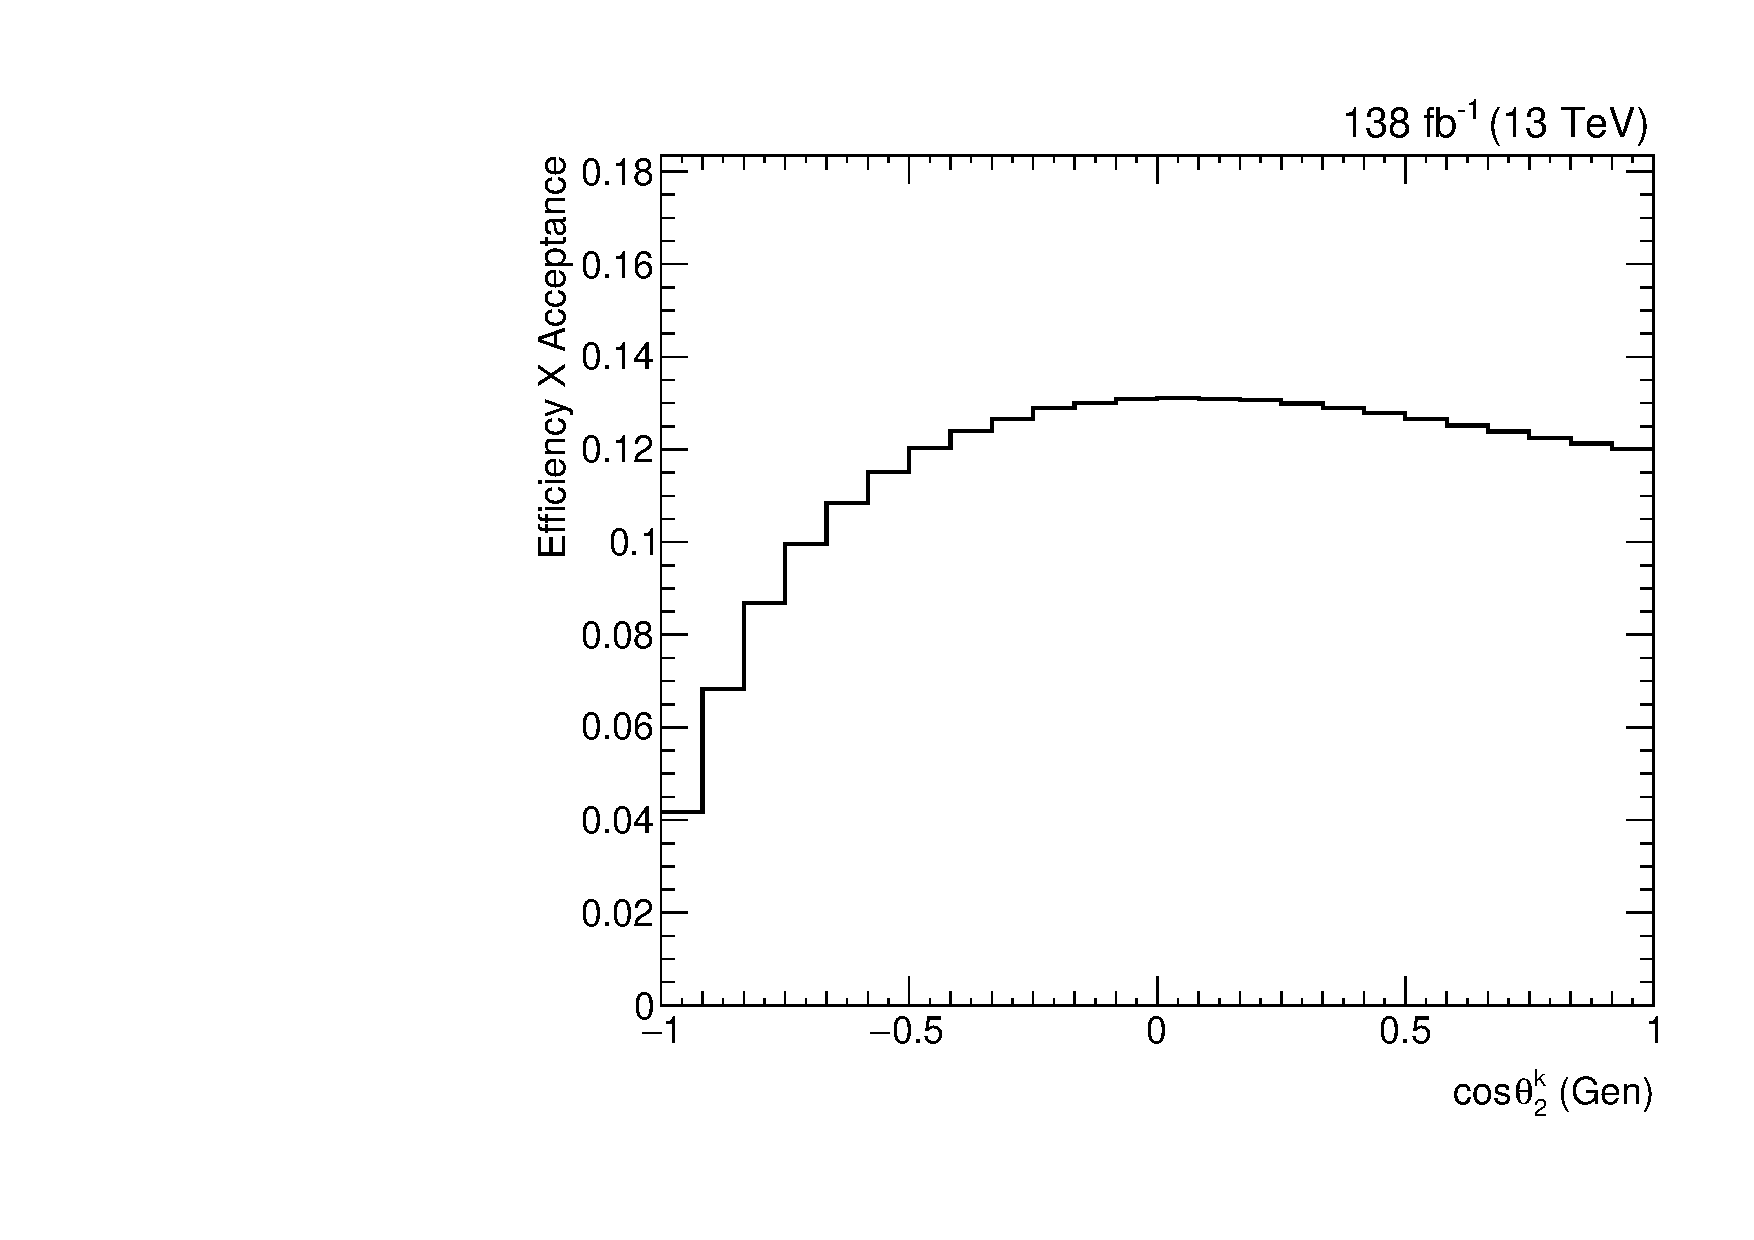
\includegraphics[width=0.32\textwidth]{fig_fullRun2UL/unfolding/combined/TotEff_b2k.pdf}
 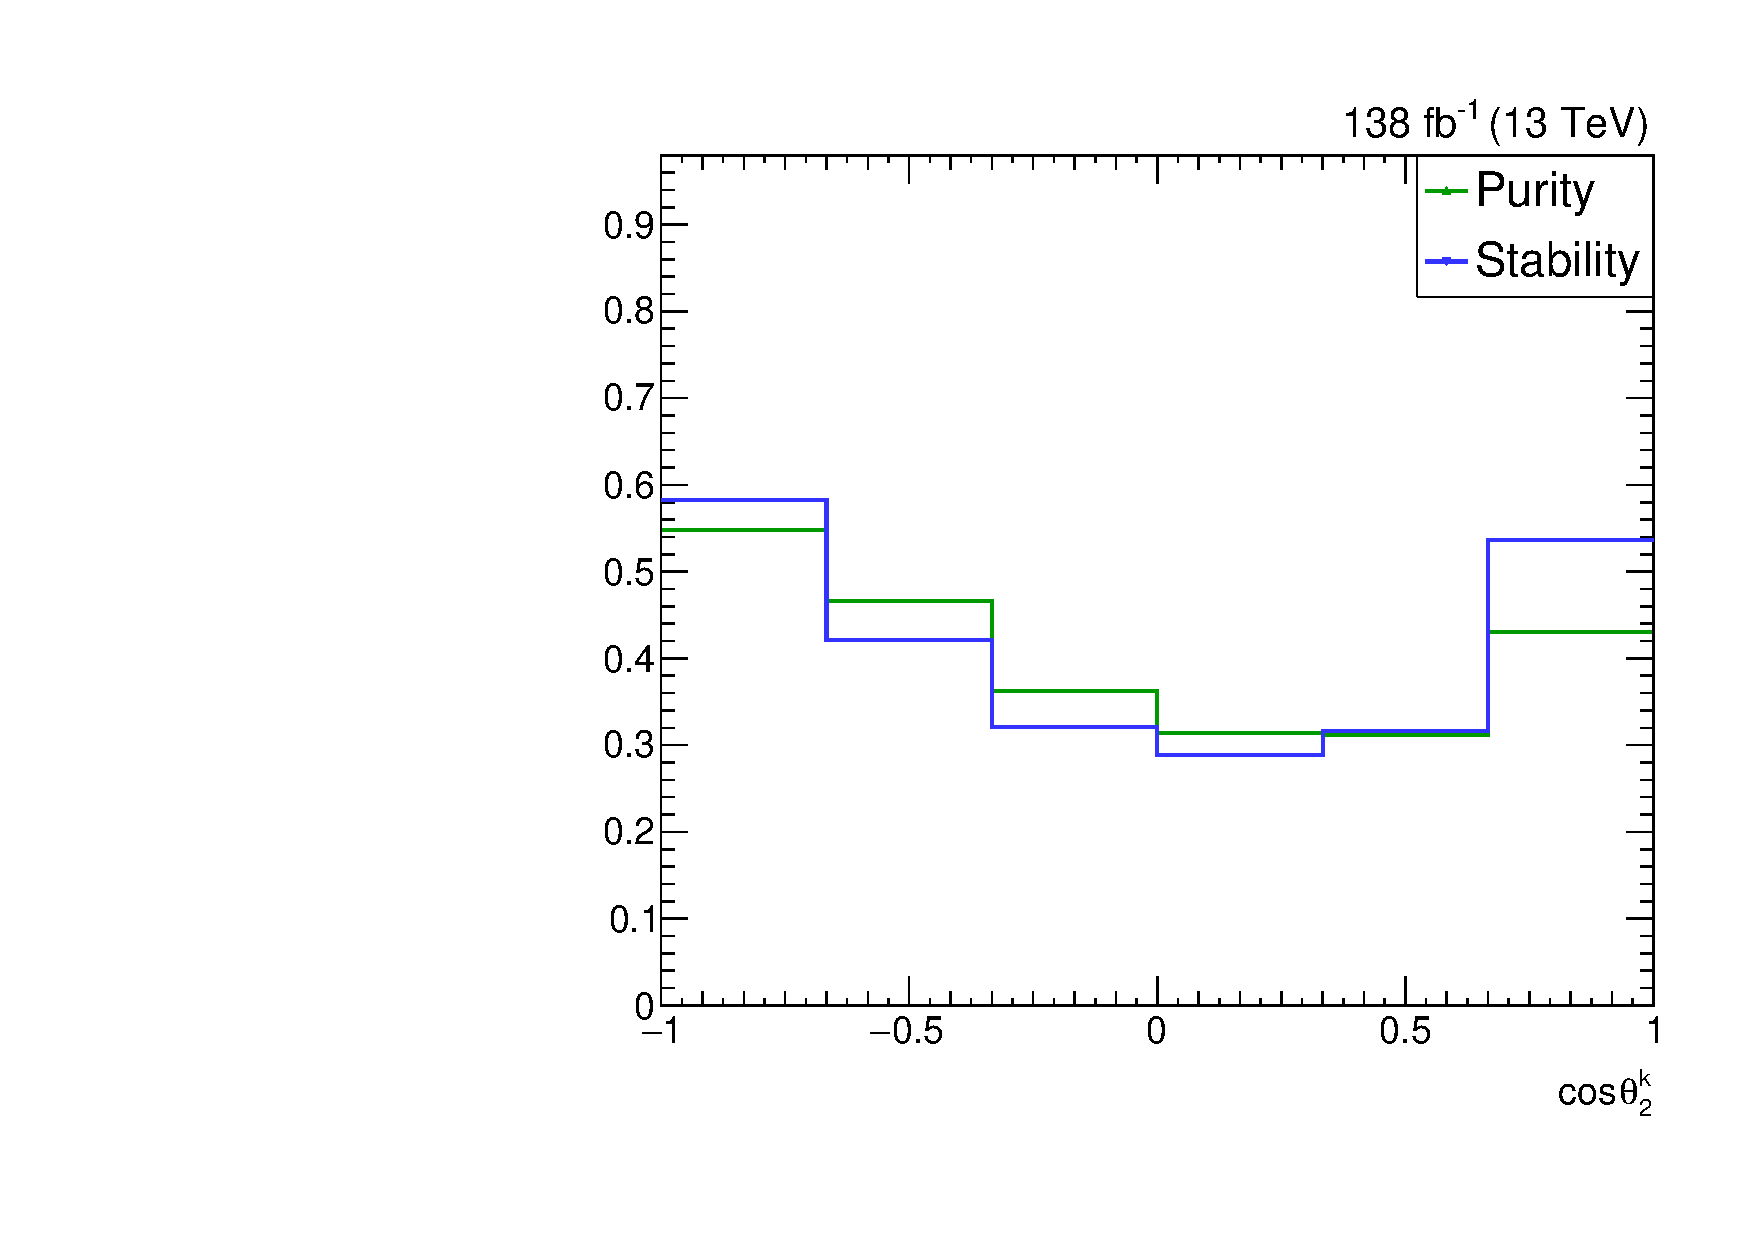
\includegraphics[width=0.32\textwidth]{fig_fullRun2UL/unfolding/combined/PurStab_b2k.pdf} \\
\caption{Reconstructed detector-level distribution (Top Left), absolute cross-section unfolded to parton-level (Top Middle), normalized cross-section unfolded to parton-level (Top Right), detector response-matrix (Bottom Left), efficiency$\times$acceptance (Bottom Middle), Purity and Stability (Bottom Right) for polarization observable $\cos\theta_{2}^{k}$, from which spin-density coefficient $B_{2}^{k}$ (sensitive to spin-density coefficient function $b_k^{-}$) is extracted.}
\label{fig:b2k}
\end{center}
\end{figure}
\clearpage
\begin{figure}[htb]
\begin{center}
 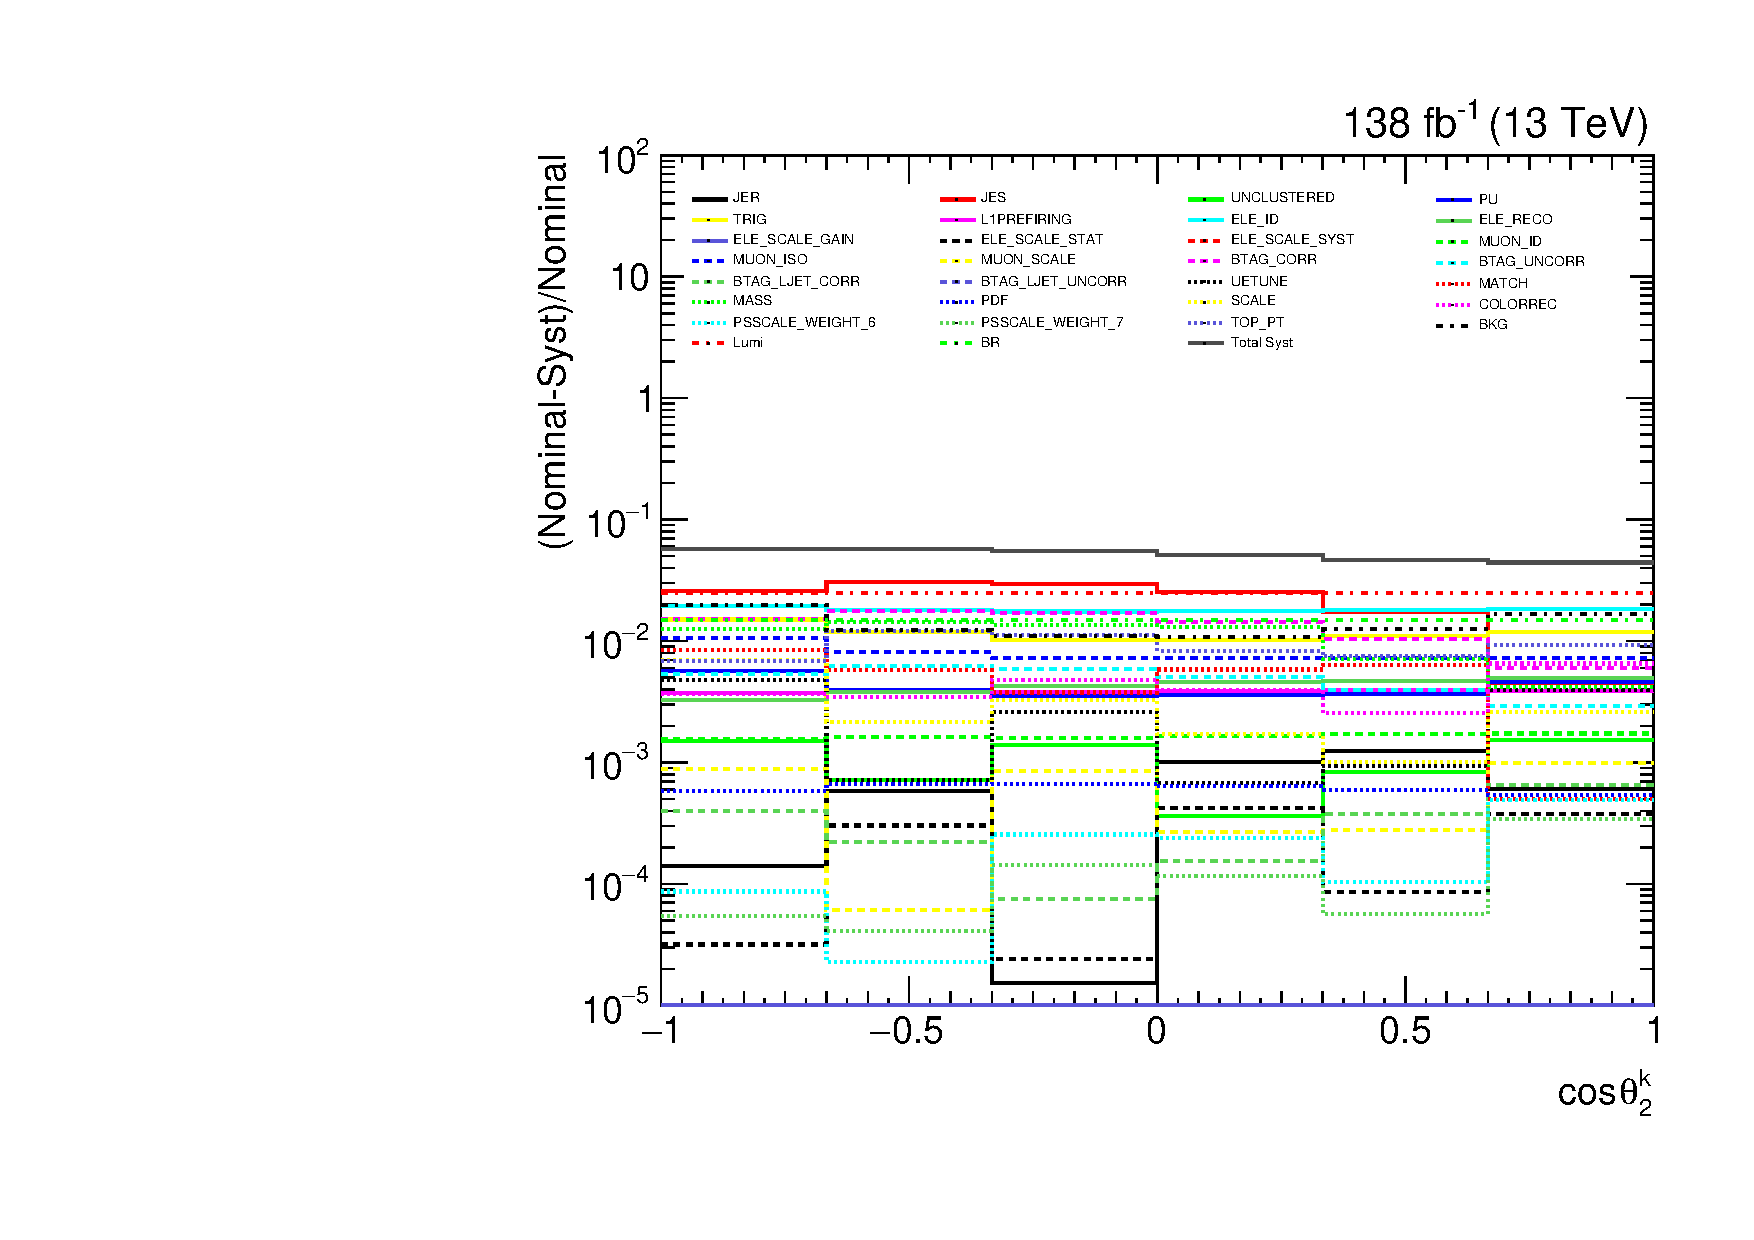
\includegraphics[width=0.32\textwidth]{fig_fullRun2UL/unfolding/combined/deltaSystCombinedlog_rebinnedB_b2k.pdf}
 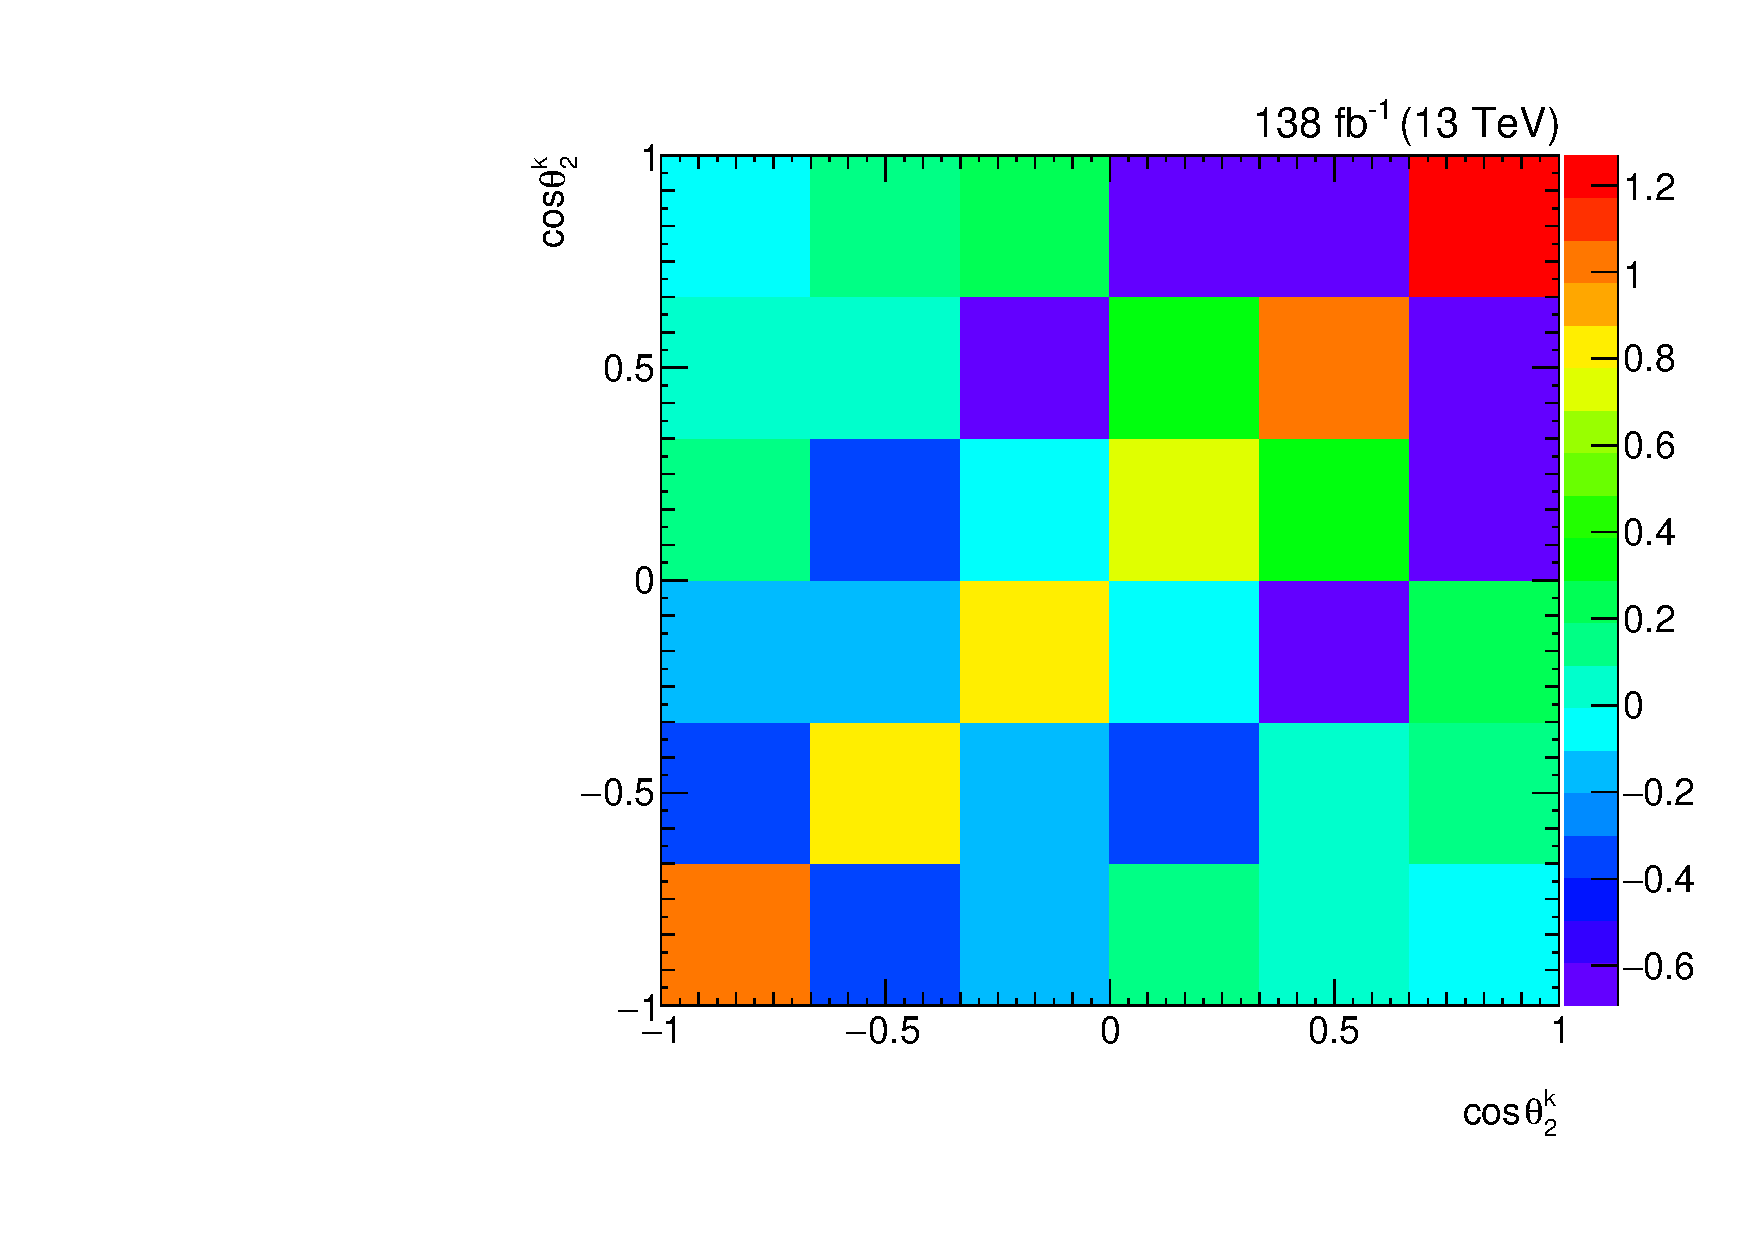
\includegraphics[width=0.32\textwidth]{fig_fullRun2UL/unfolding/combined/StatCovMatrix_rebinnedB_b2k.pdf}
 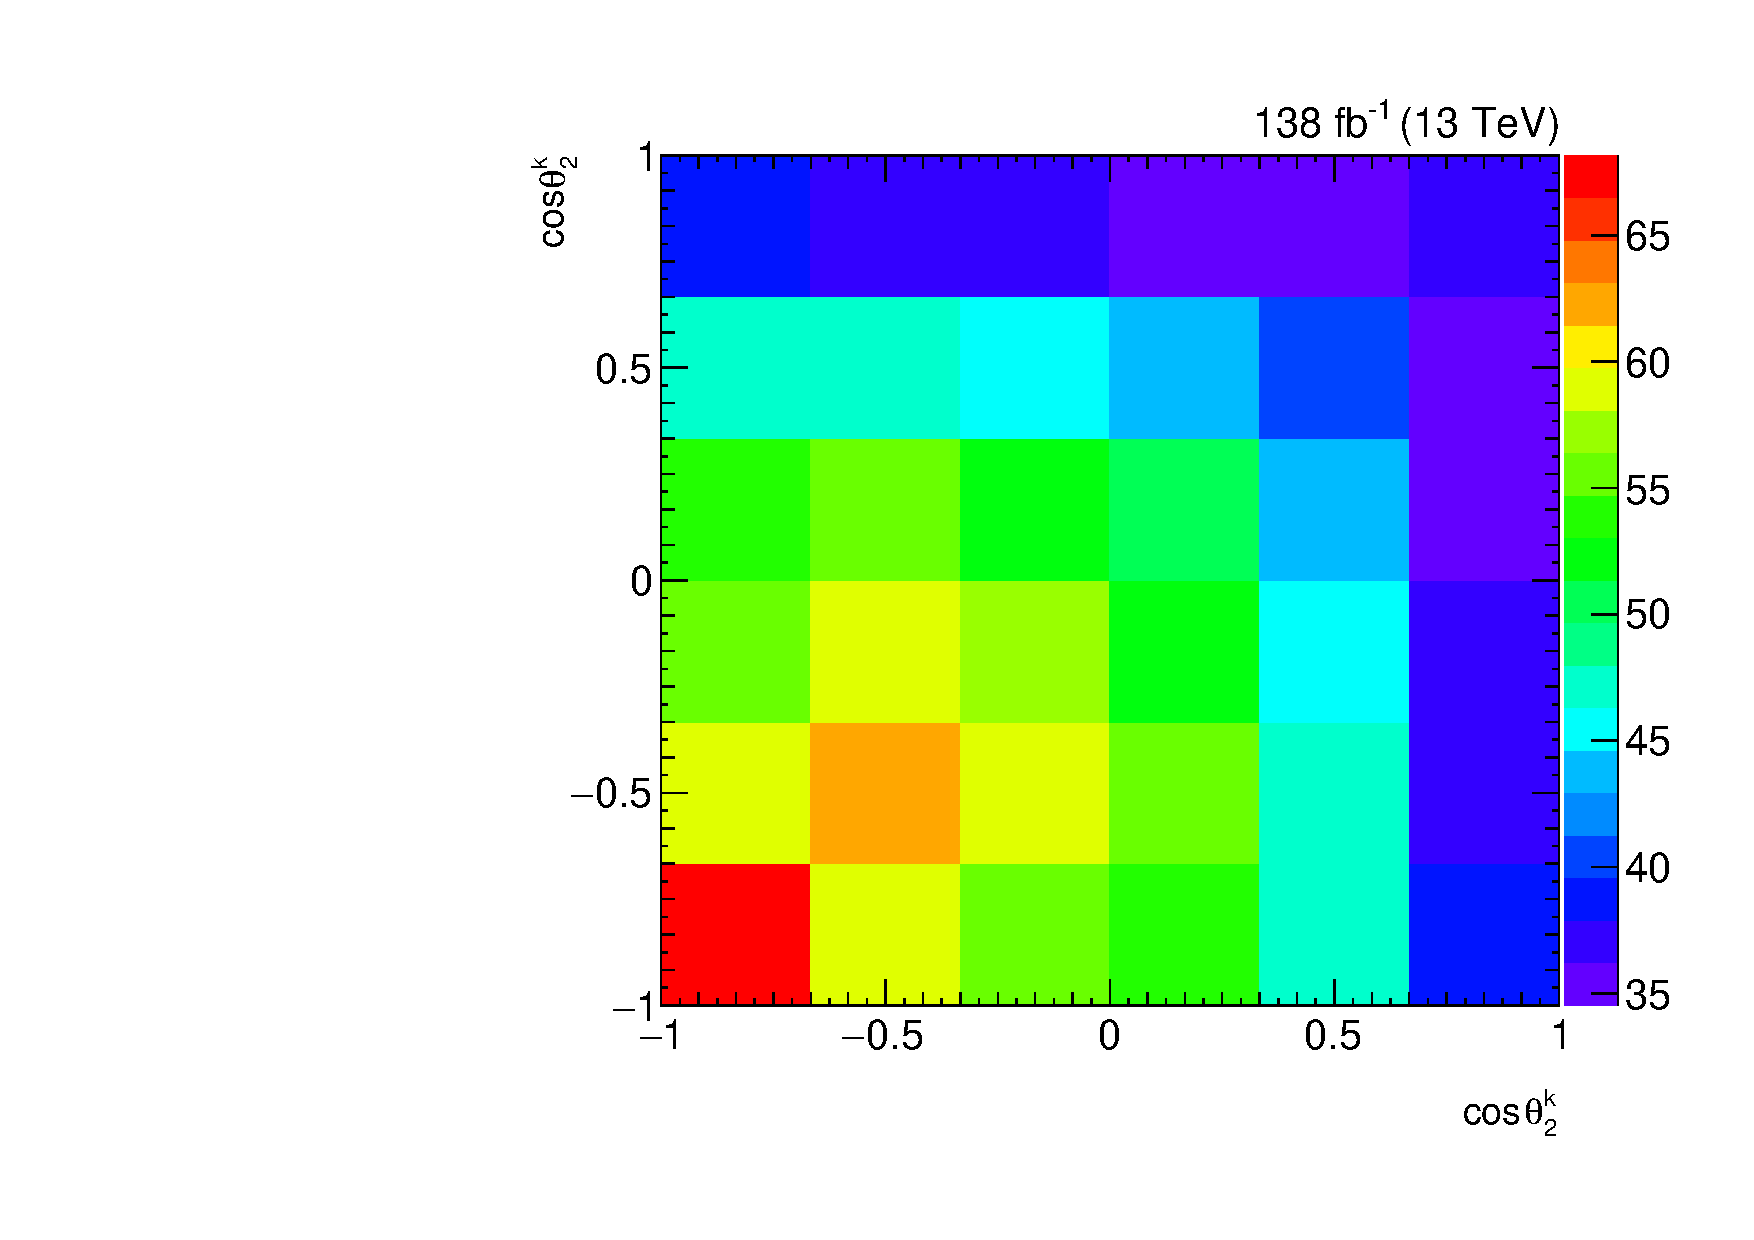
\includegraphics[width=0.32\textwidth]{fig_fullRun2UL/unfolding/combined/TotalSystCovMatrix_rebinnedB_b2k.pdf} \\
 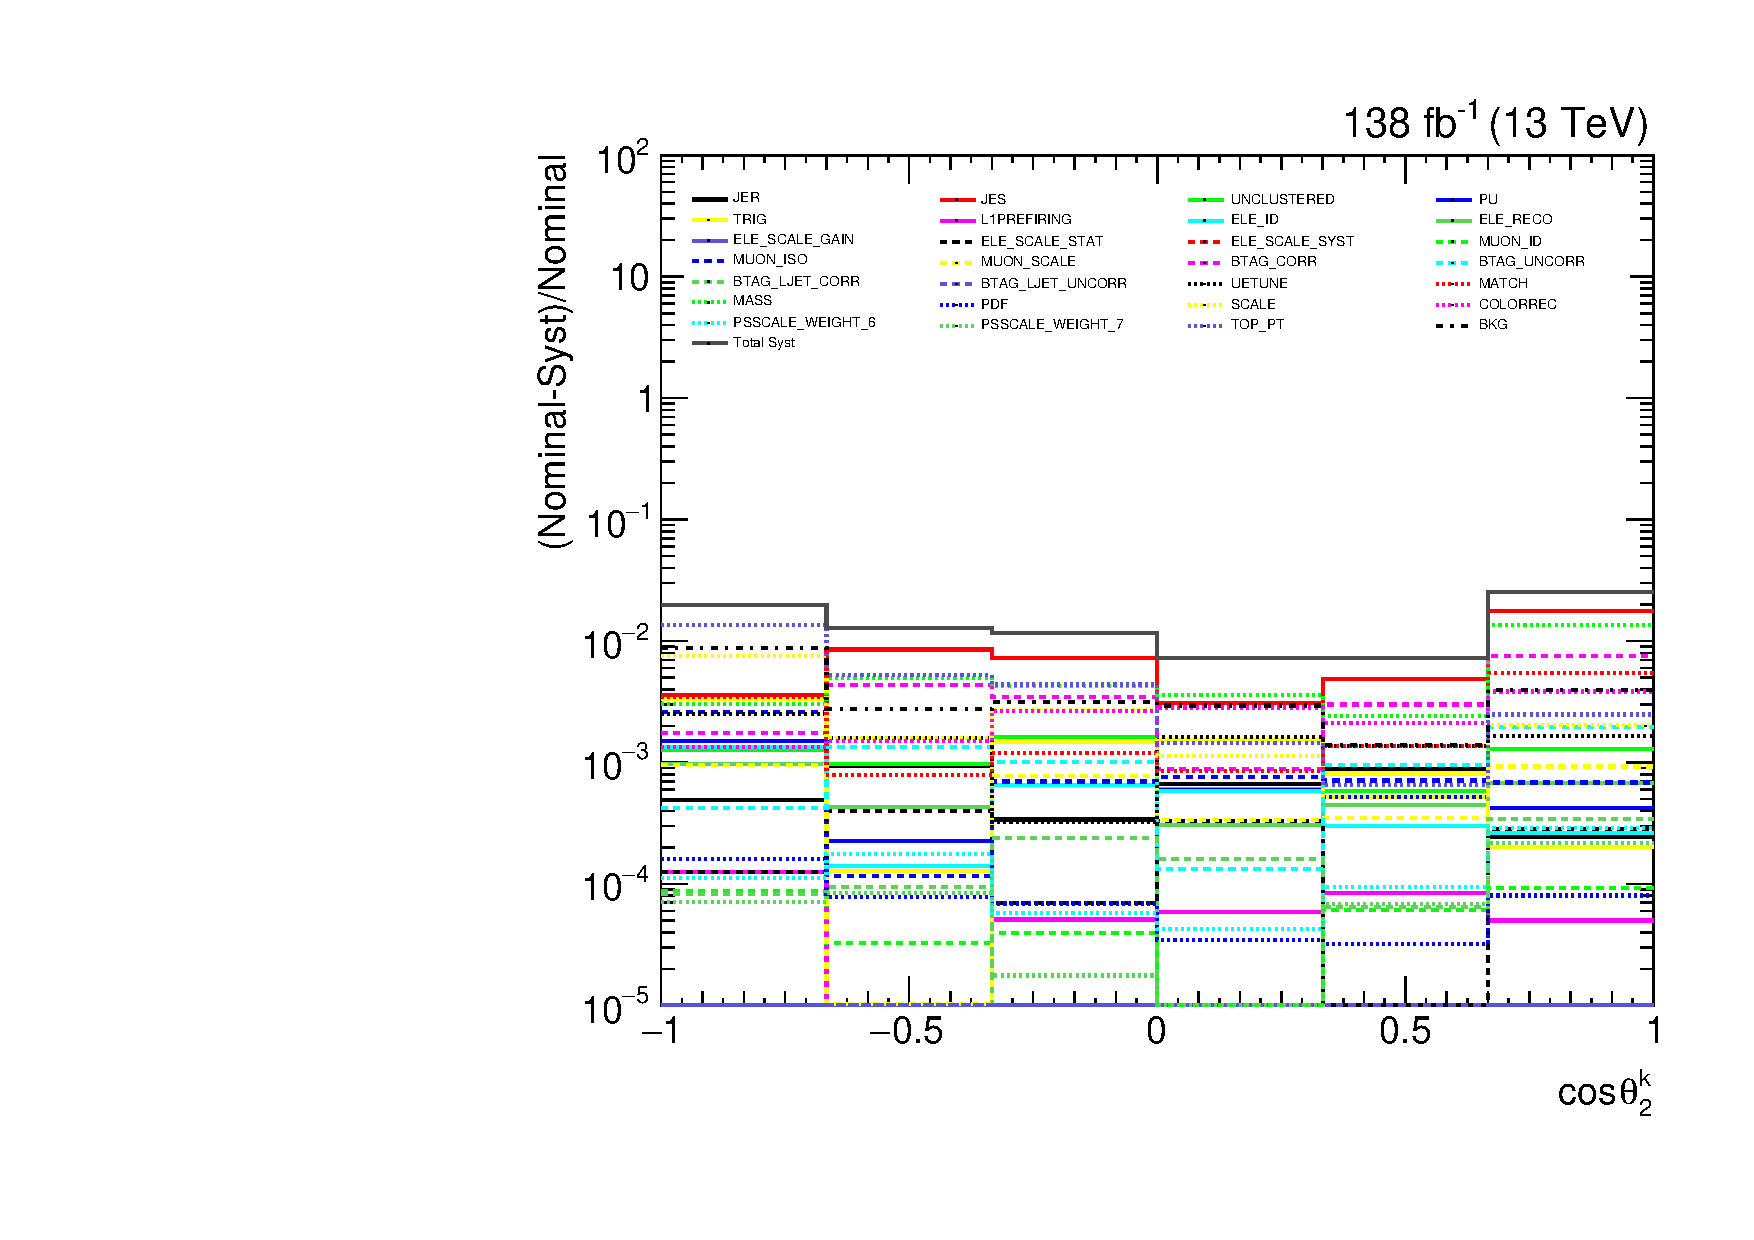
\includegraphics[width=0.32\textwidth]{fig_fullRun2UL/unfolding/combined/deltaSystCombinedlogNorm_rebinnedB_b2k.pdf}
 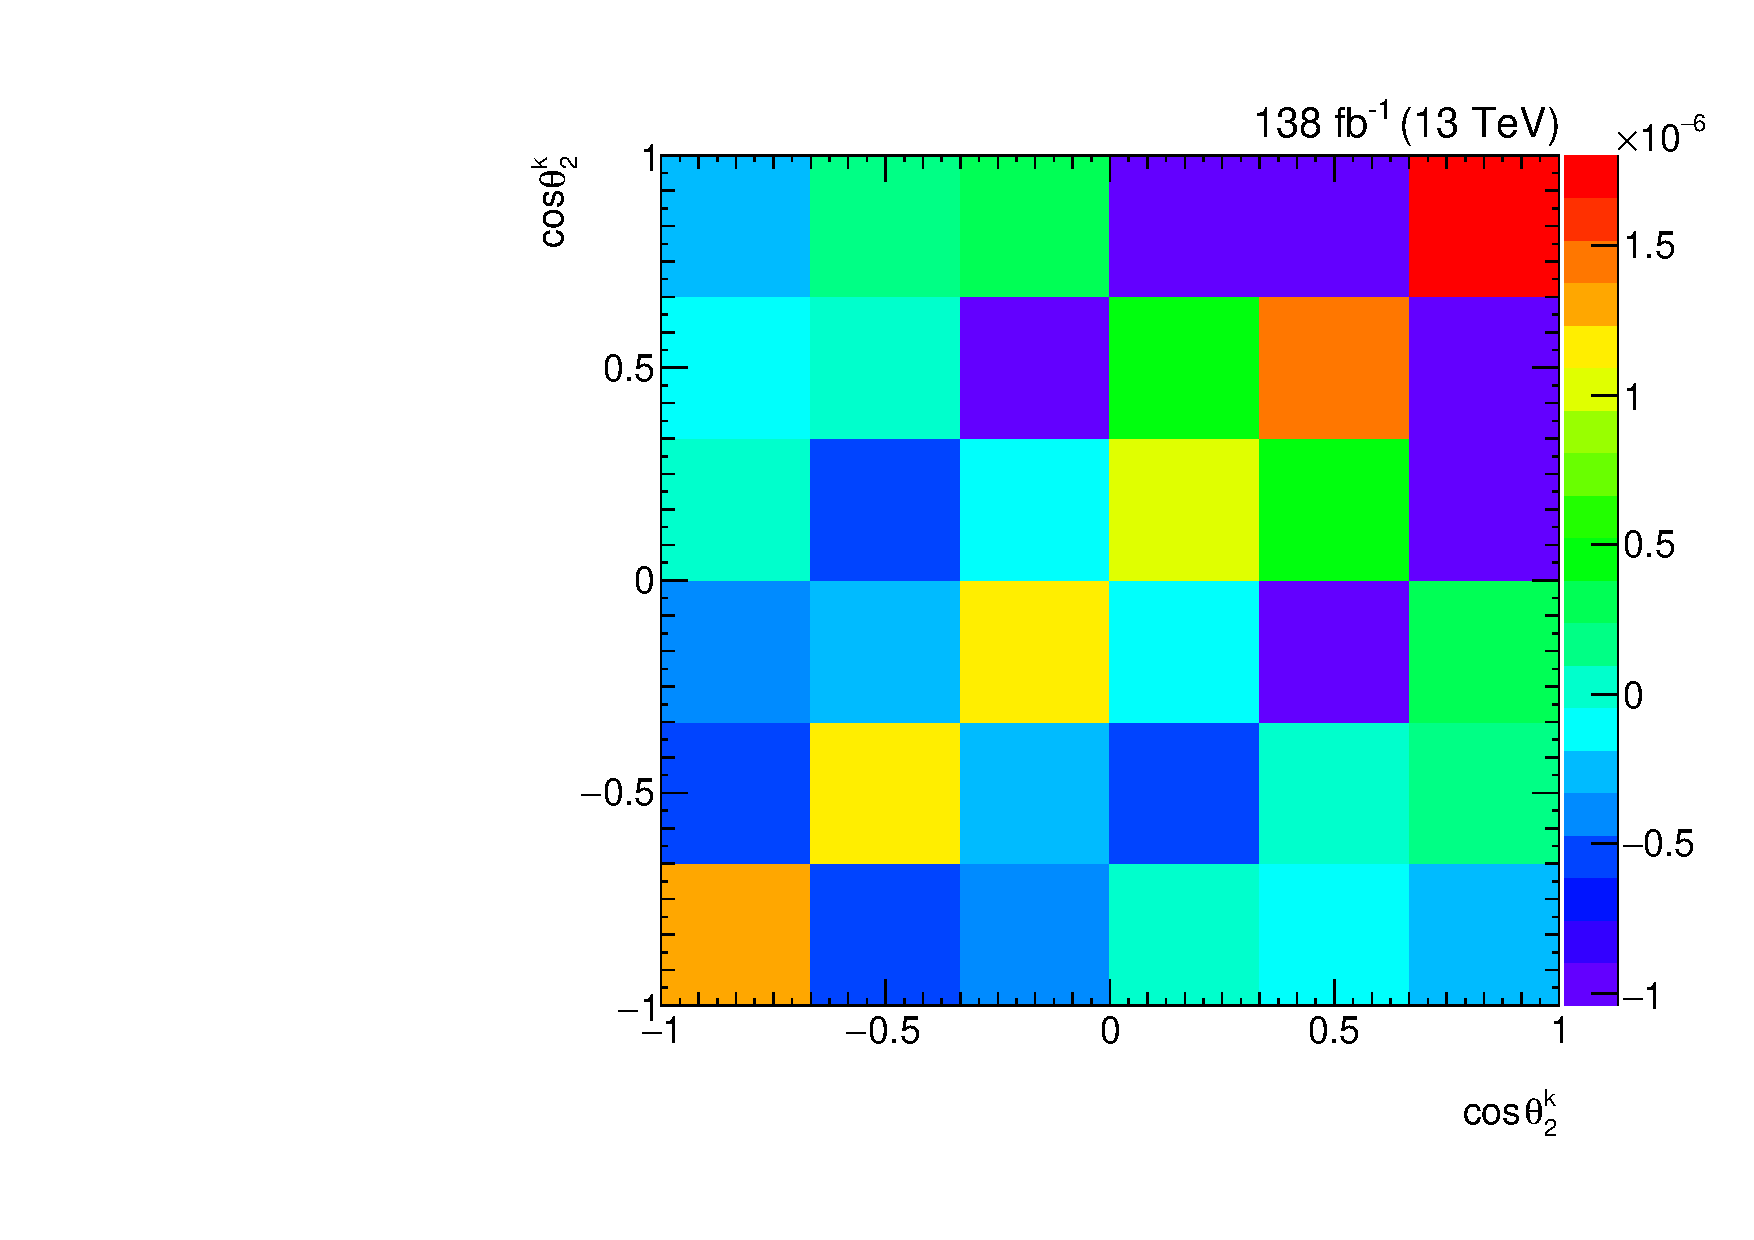
\includegraphics[width=0.32\textwidth]{fig_fullRun2UL/unfolding/combined/StatCovMatrixNorm_rebinnedB_b2k.pdf}
 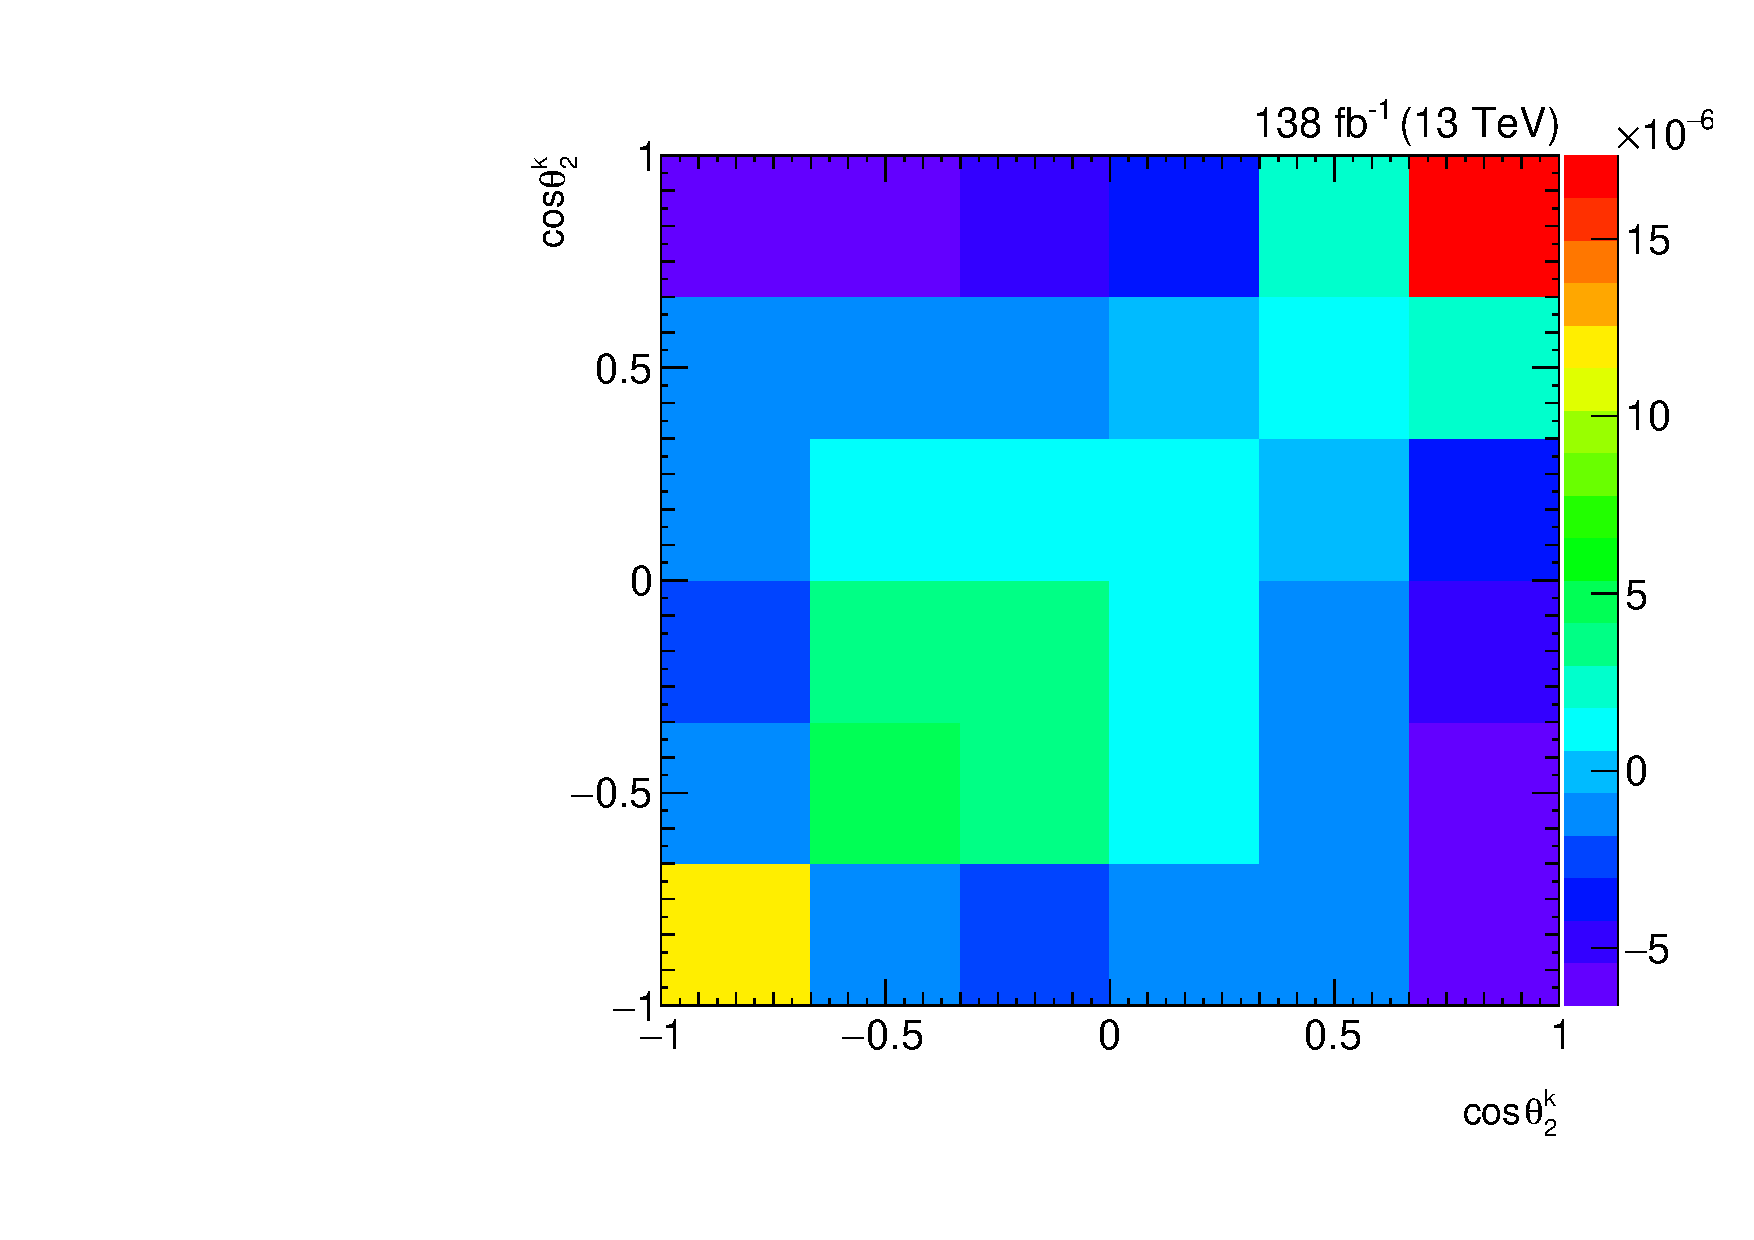
\includegraphics[width=0.32\textwidth]{fig_fullRun2UL/unfolding/combined/TotalSystCovMatrixNorm_rebinnedB_b2k.pdf} \\
\caption{Unfolded-cross section breakdown of uncertainties (Top Left), unfolded cross-section statistical covariance matrix (Top Middle), unfolded cross-section total systematic covariance matrix (Top Right), normalized unfolded-cross section breakdown of uncertainties (Bottom Left), normalized unfolded cross-section statistical covariance matrix (Bottom Middle), normalized unfolded cross-section total systematic covariance matrix (Bottom Right) for polarization observable $\cos\theta_{2}^{k}$.}
\label{fig:b2k_uncertainties}
\end{center}
\end{figure}
\clearpage
\begin{figure}[htb]
\begin{center}
 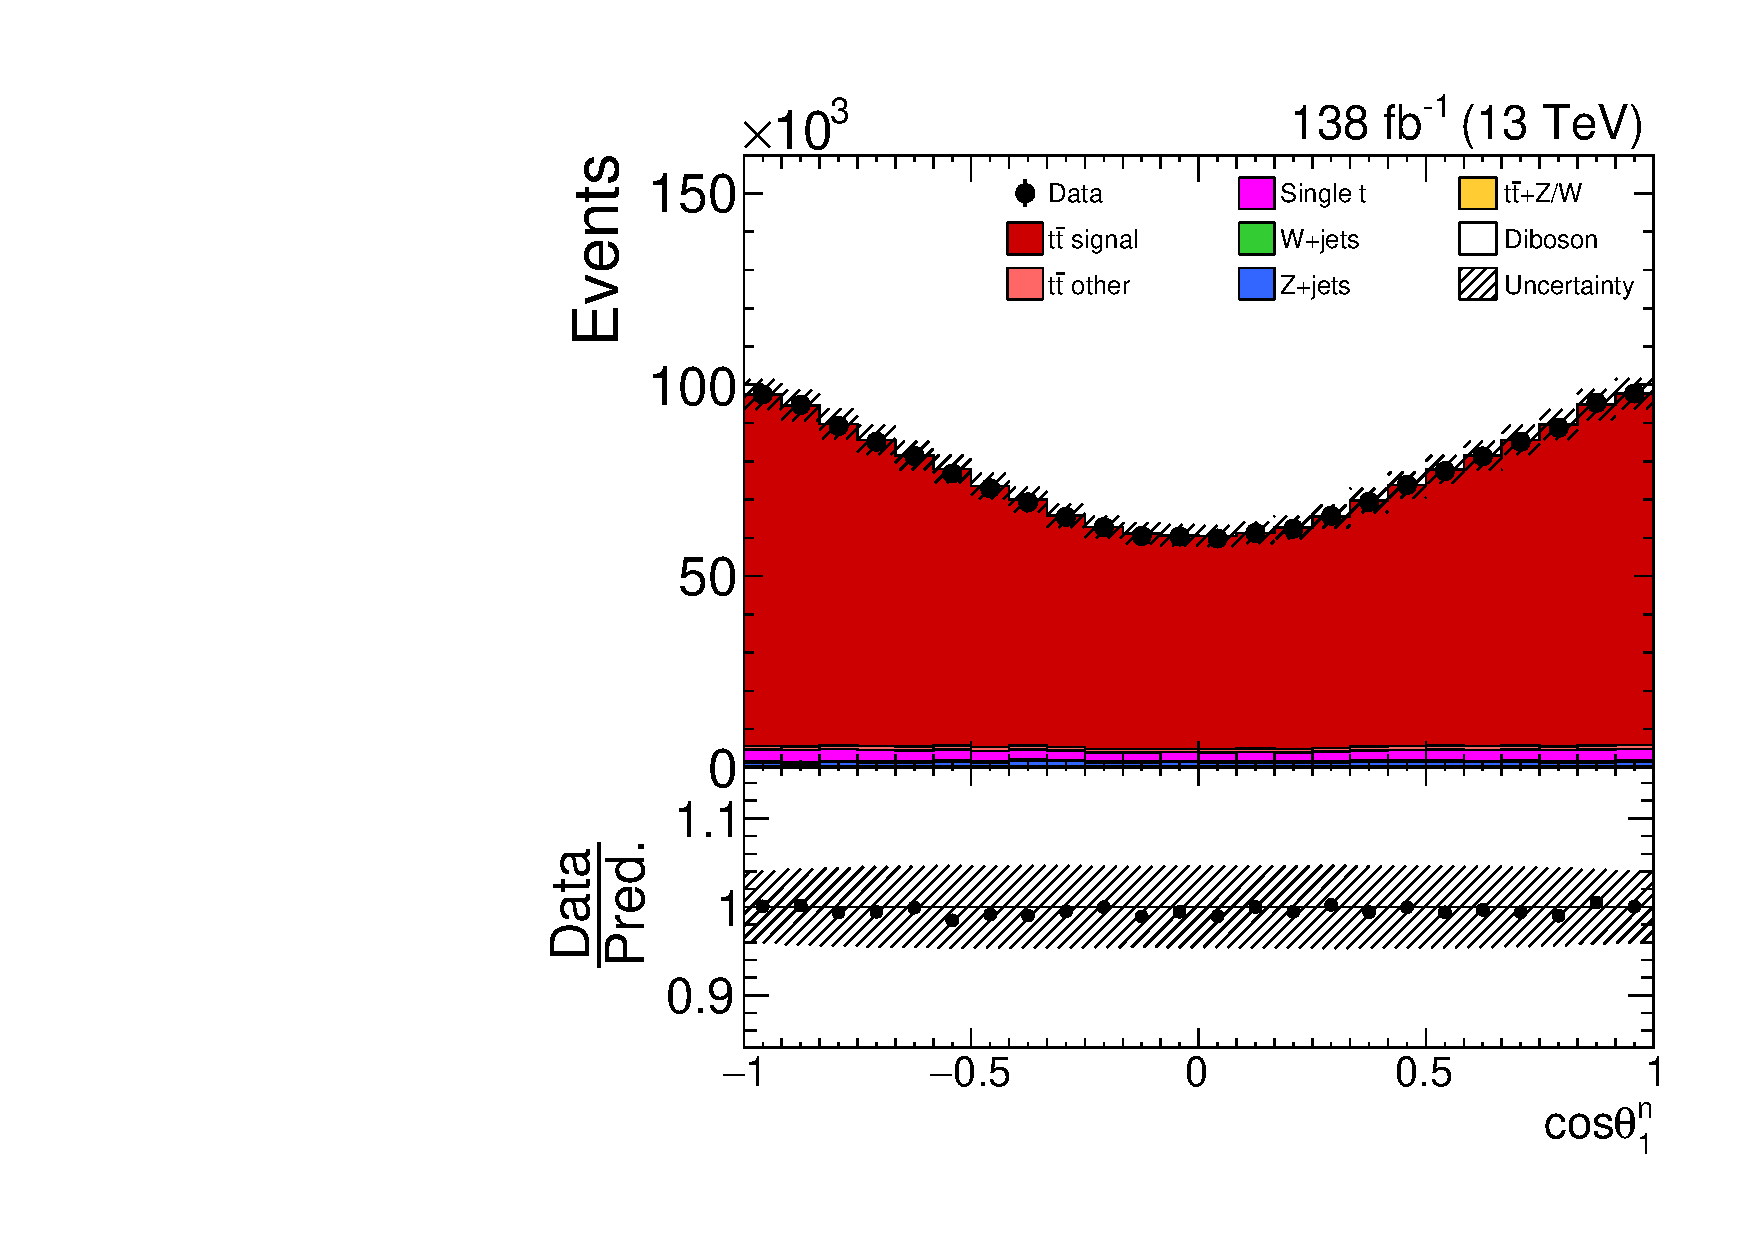
\includegraphics[width=0.32\textwidth]{fig_fullRun2UL/controlplots/combined/Hyp_AntiLeptonBn.pdf}
 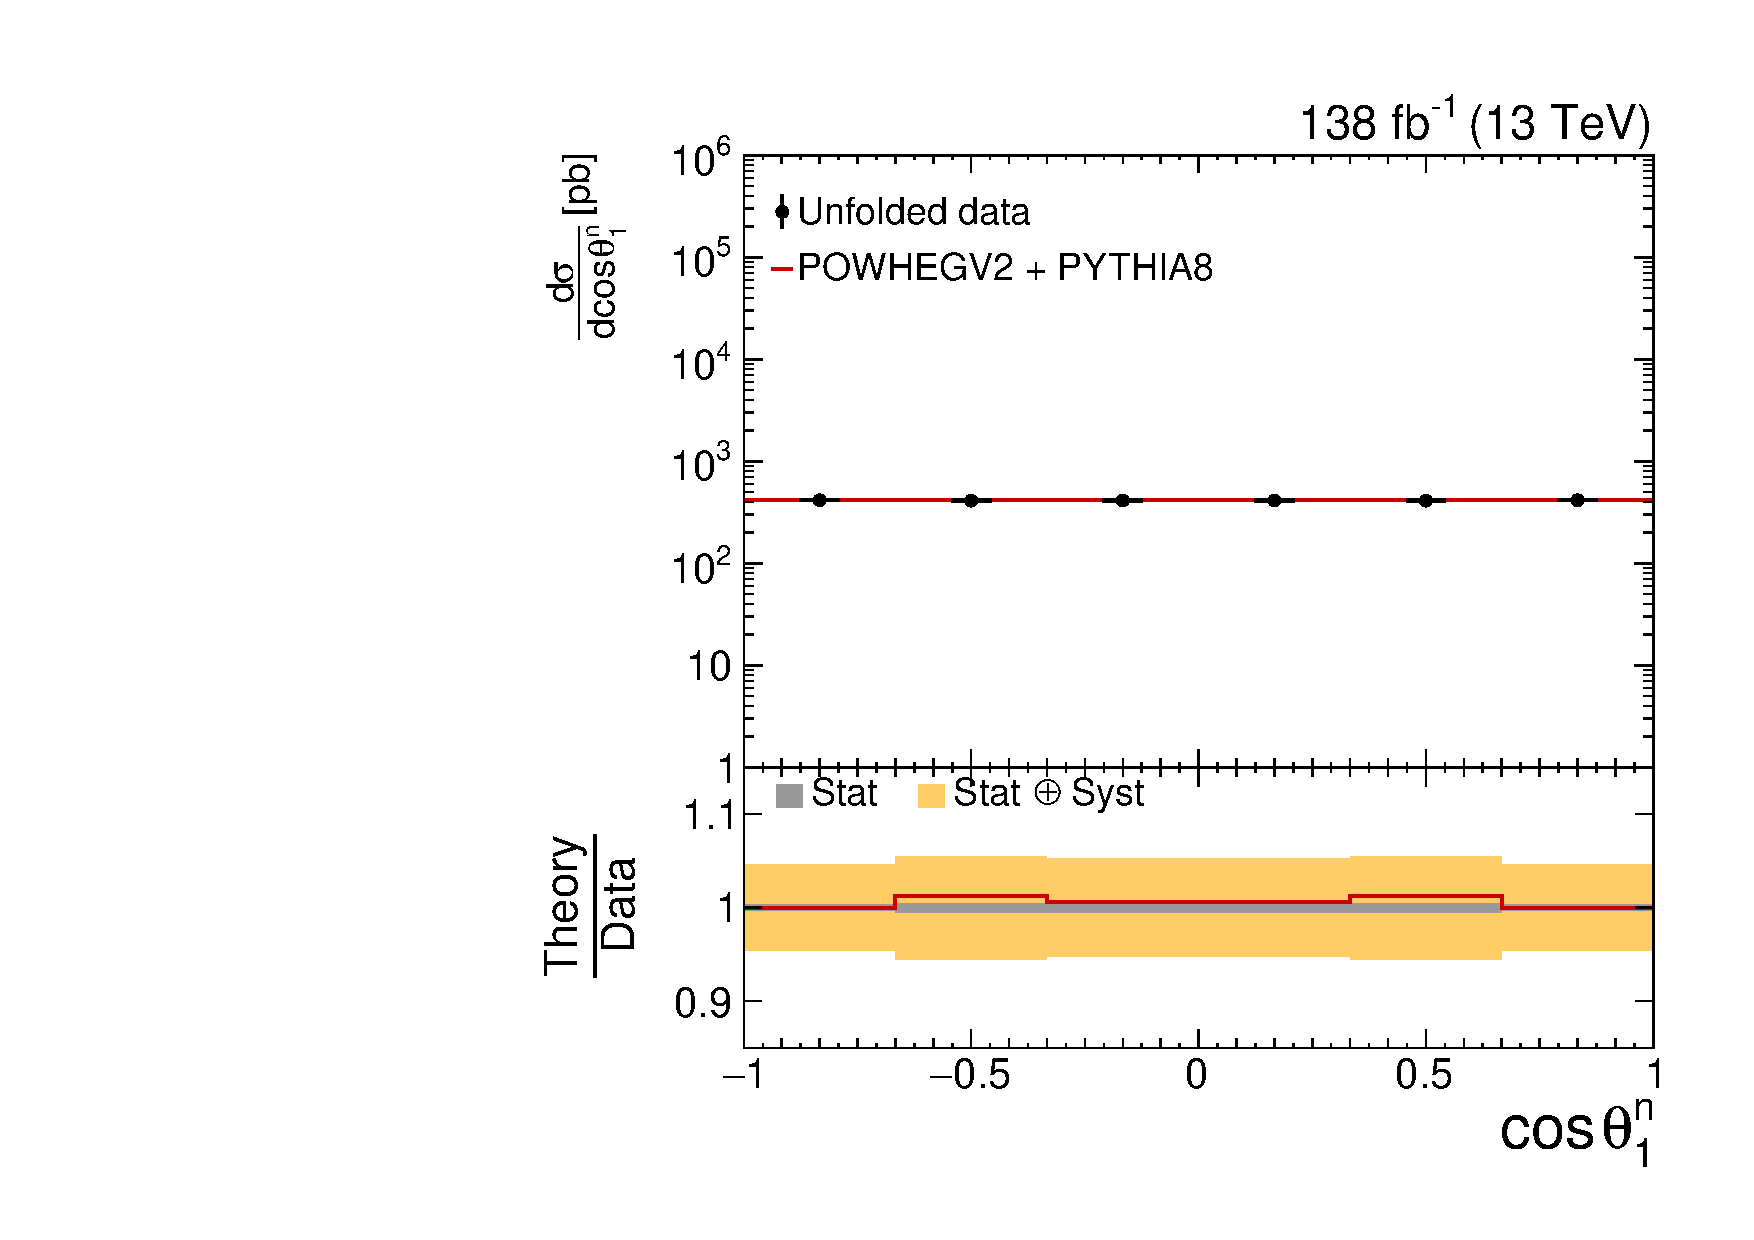
\includegraphics[width=0.32\textwidth]{fig_fullRun2UL/unfolding/combined/UnfoldedResults_b1n.pdf}
 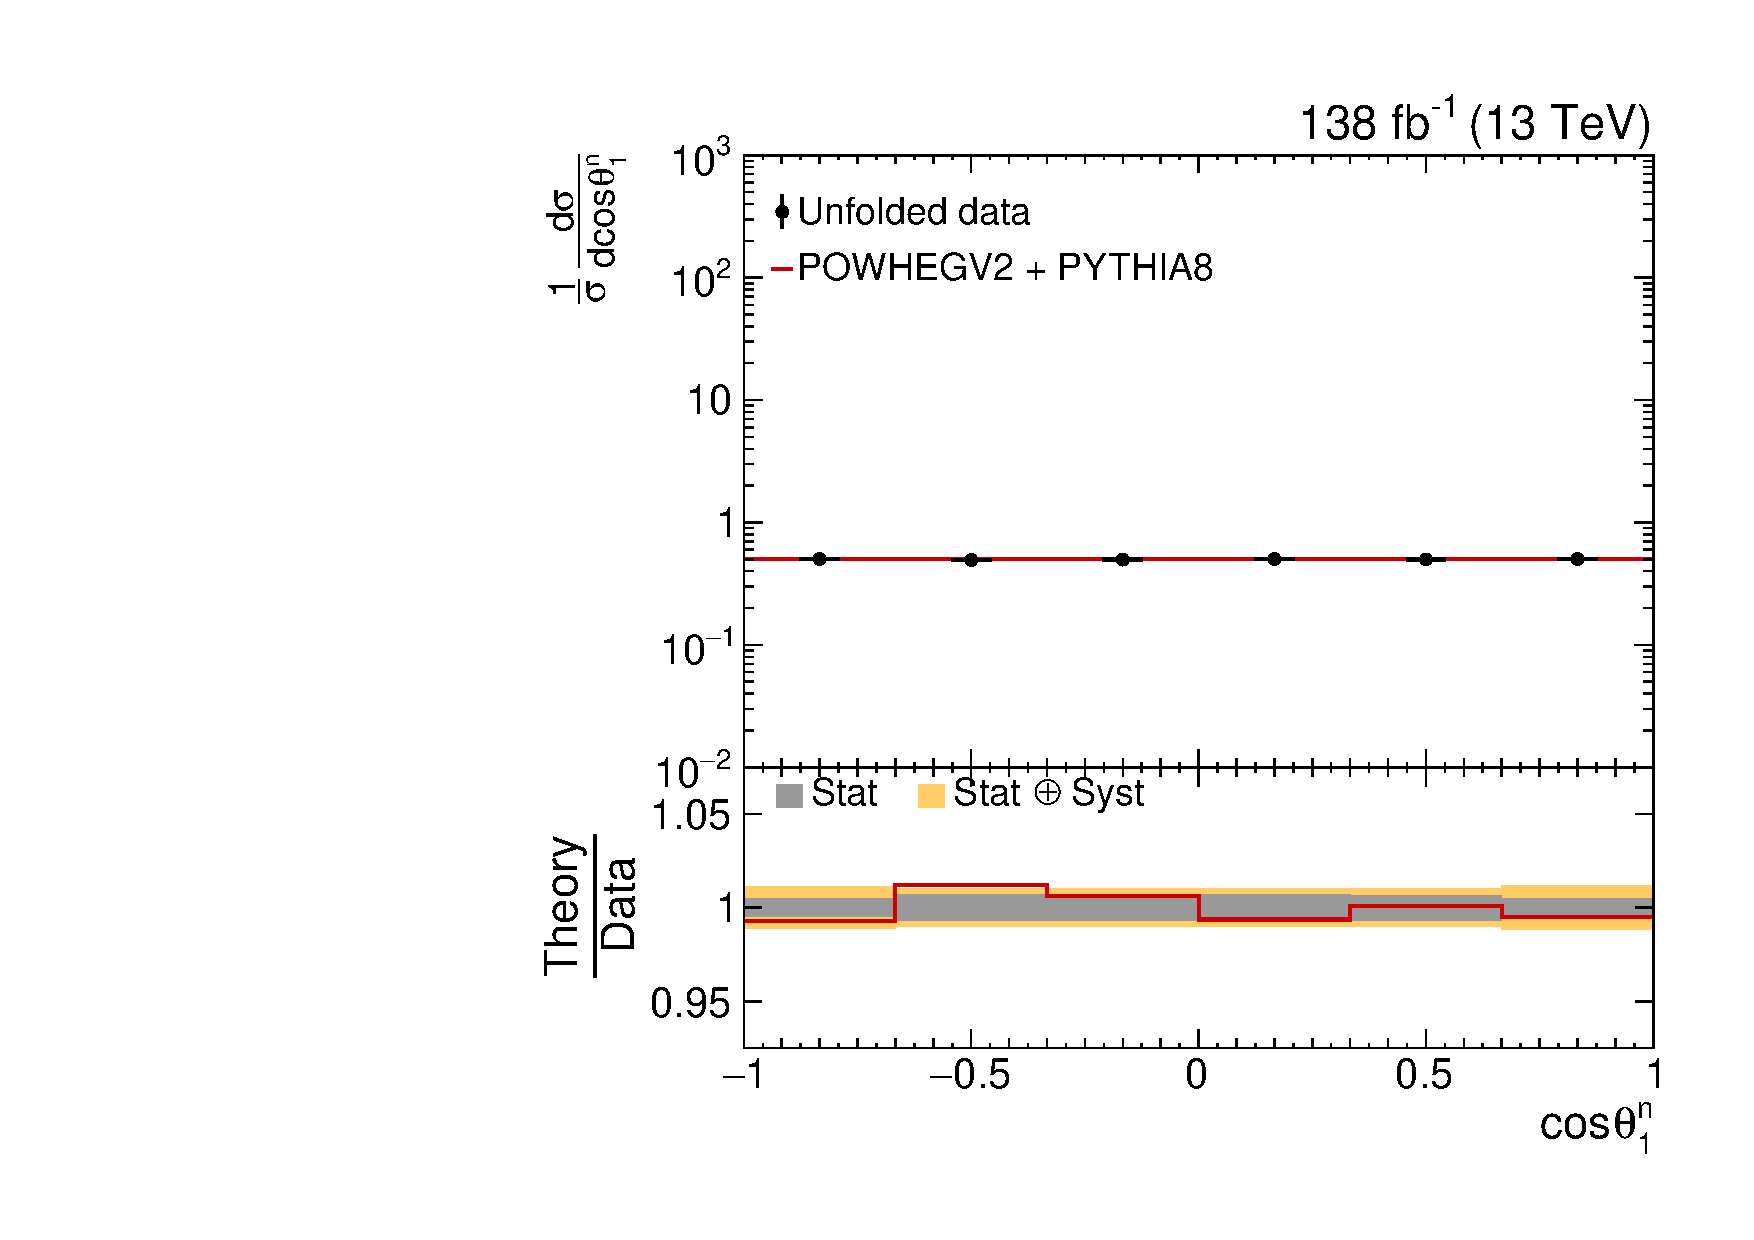
\includegraphics[width=0.32\textwidth]{fig_fullRun2UL/unfolding/combined/UnfoldedResultsNorm_b1n.pdf} \\
 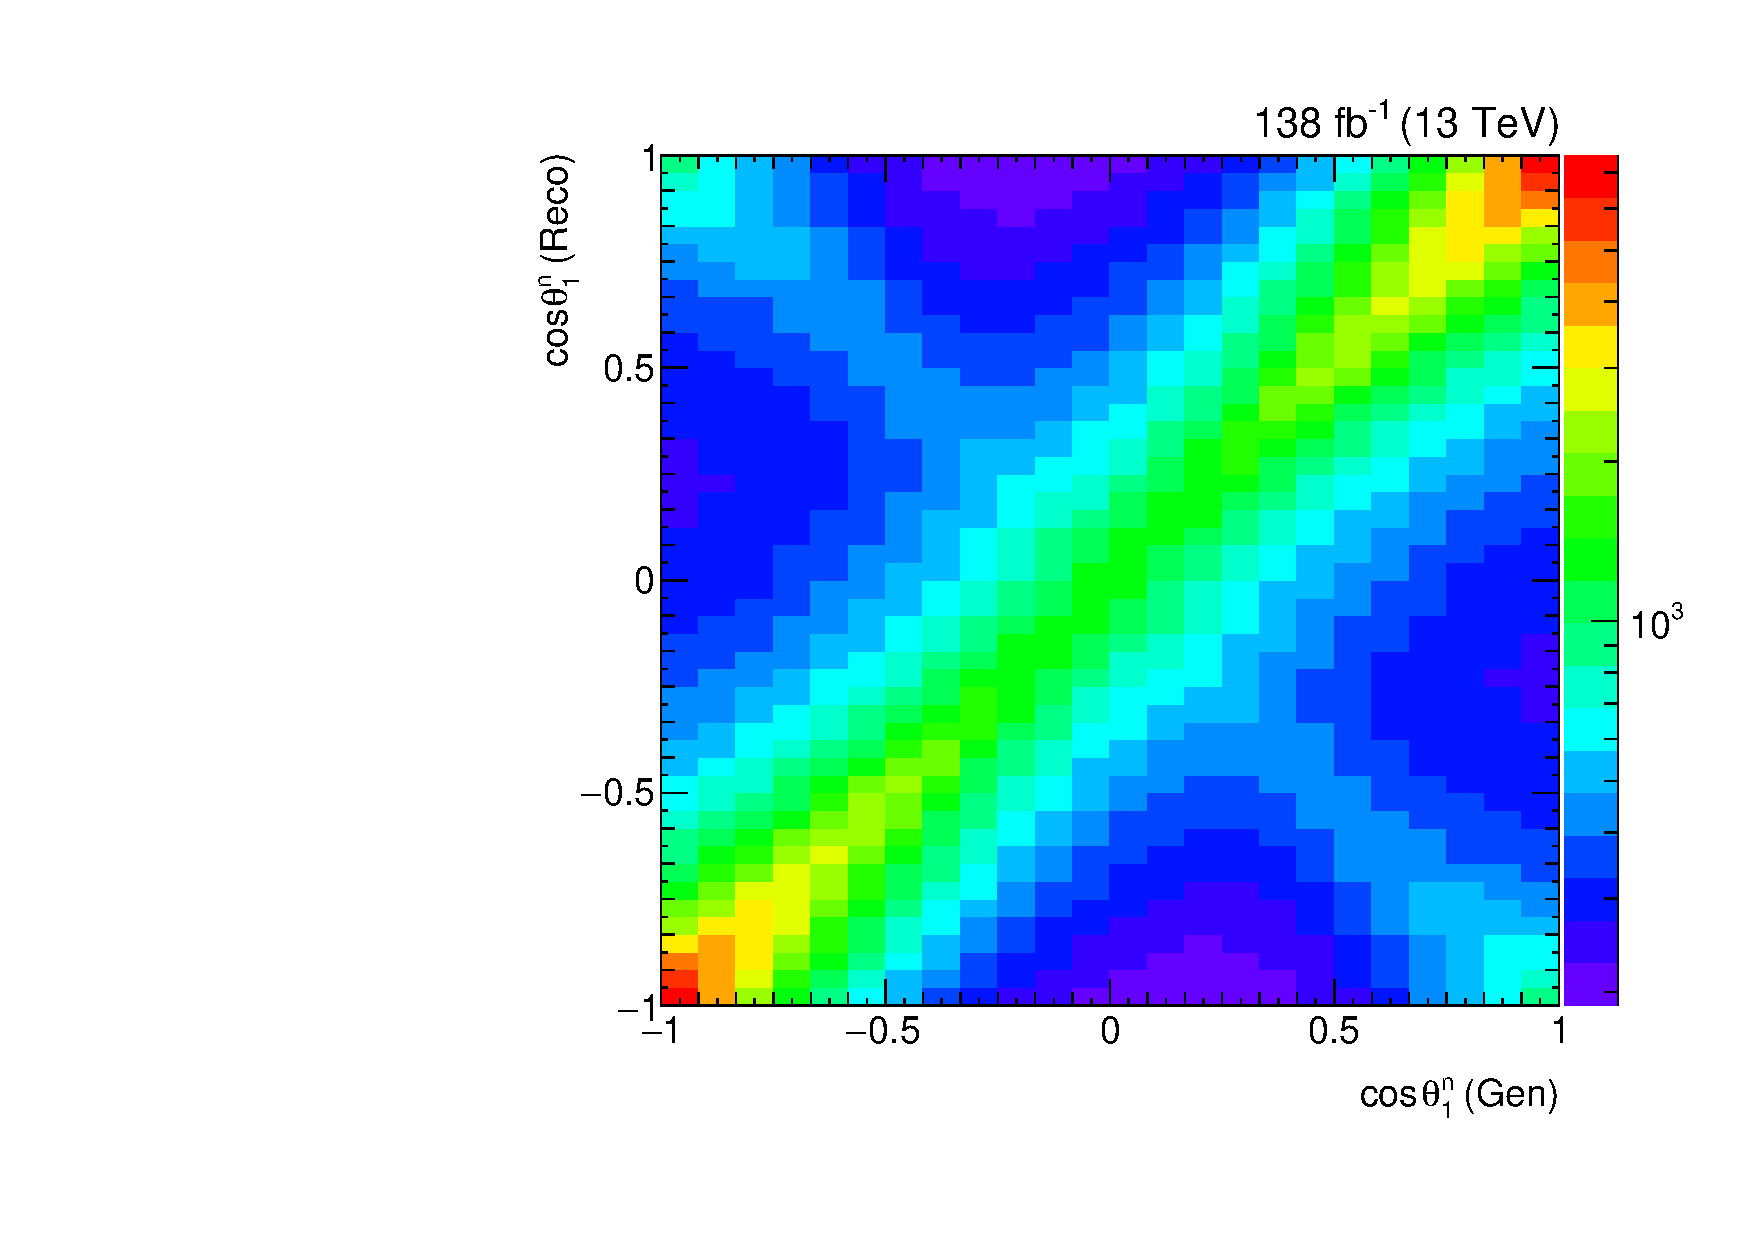
\includegraphics[width=0.32\textwidth]{fig_fullRun2UL/unfolding/combined/ResponseMatrix_b1n.pdf}
 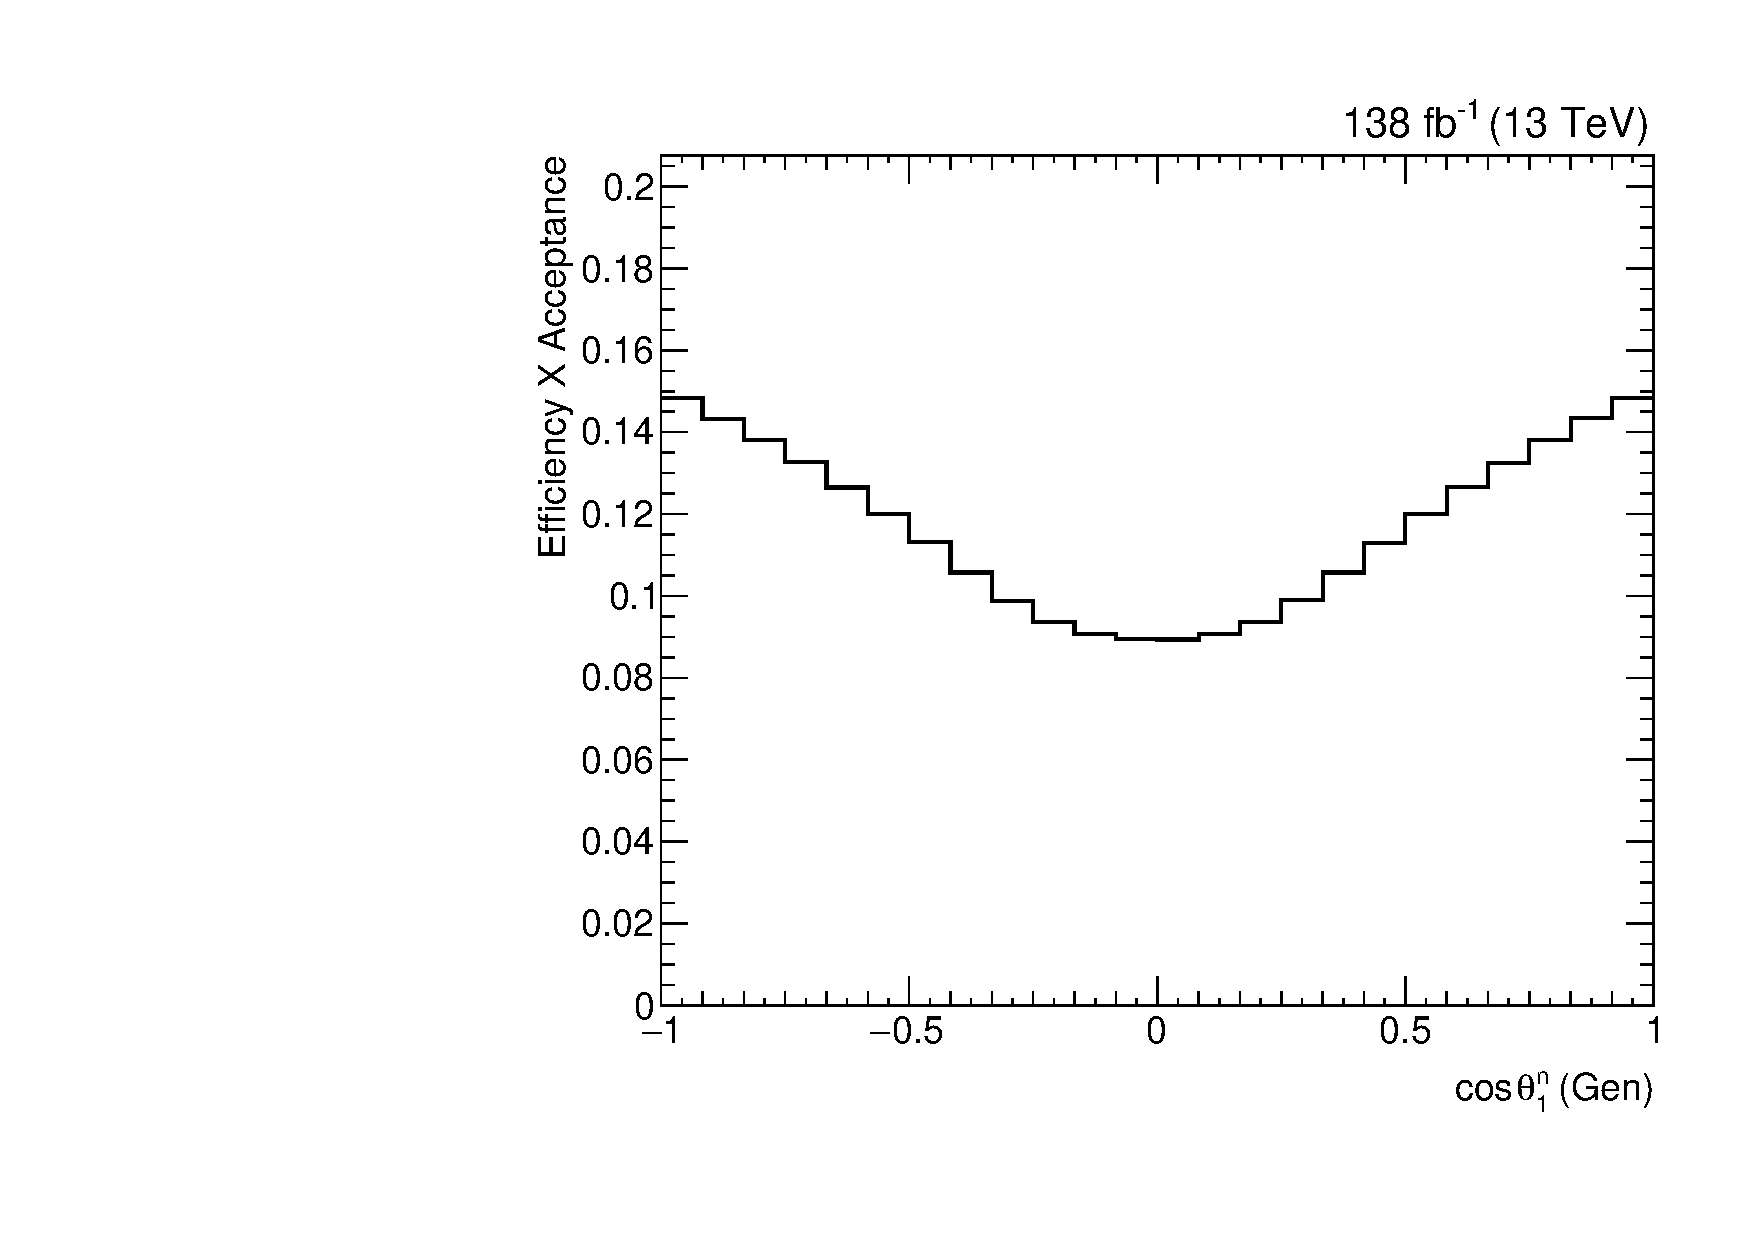
\includegraphics[width=0.32\textwidth]{fig_fullRun2UL/unfolding/combined/TotEff_b1n.pdf}
 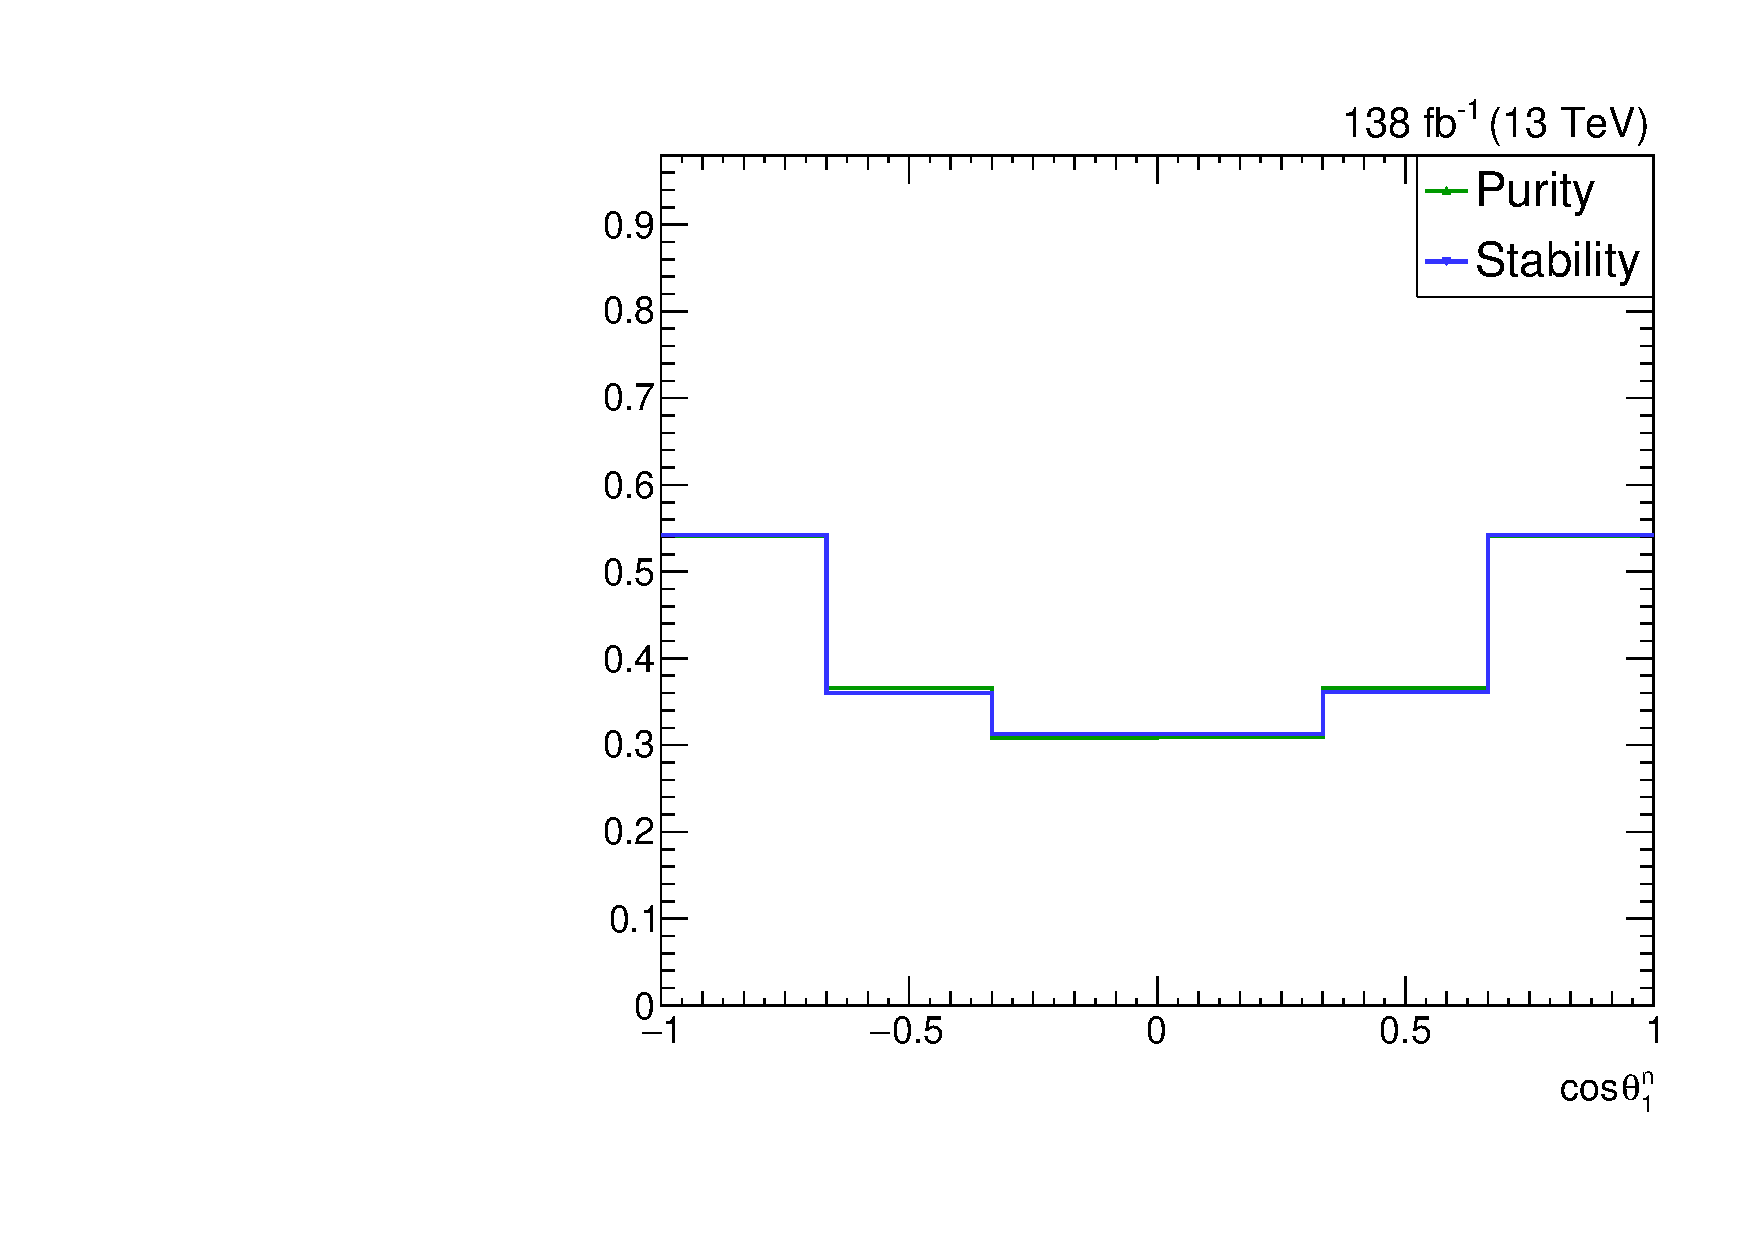
\includegraphics[width=0.32\textwidth]{fig_fullRun2UL/unfolding/combined/PurStab_b1n.pdf} \\
\caption{Reconstructed detector-level distribution (Top Left), absolute cross-section unfolded to parton-level (Top Middle), normalized cross-section unfolded to parton-level (Top Right), detector response-matrix (Bottom Left), efficiency$\times$acceptance (Bottom Middle), Purity and Stability (Bottom Right) for polarization observable $\cos\theta_{1}^{n}$, from which spin-density coefficient $B_{1}^{n}$ (sensitive to spin-density coefficient function $b_n^{+}$) is extracted.}
\label{fig:b1n}
\end{center}
\end{figure}
\clearpage
\begin{figure}[htb]
\begin{center}
 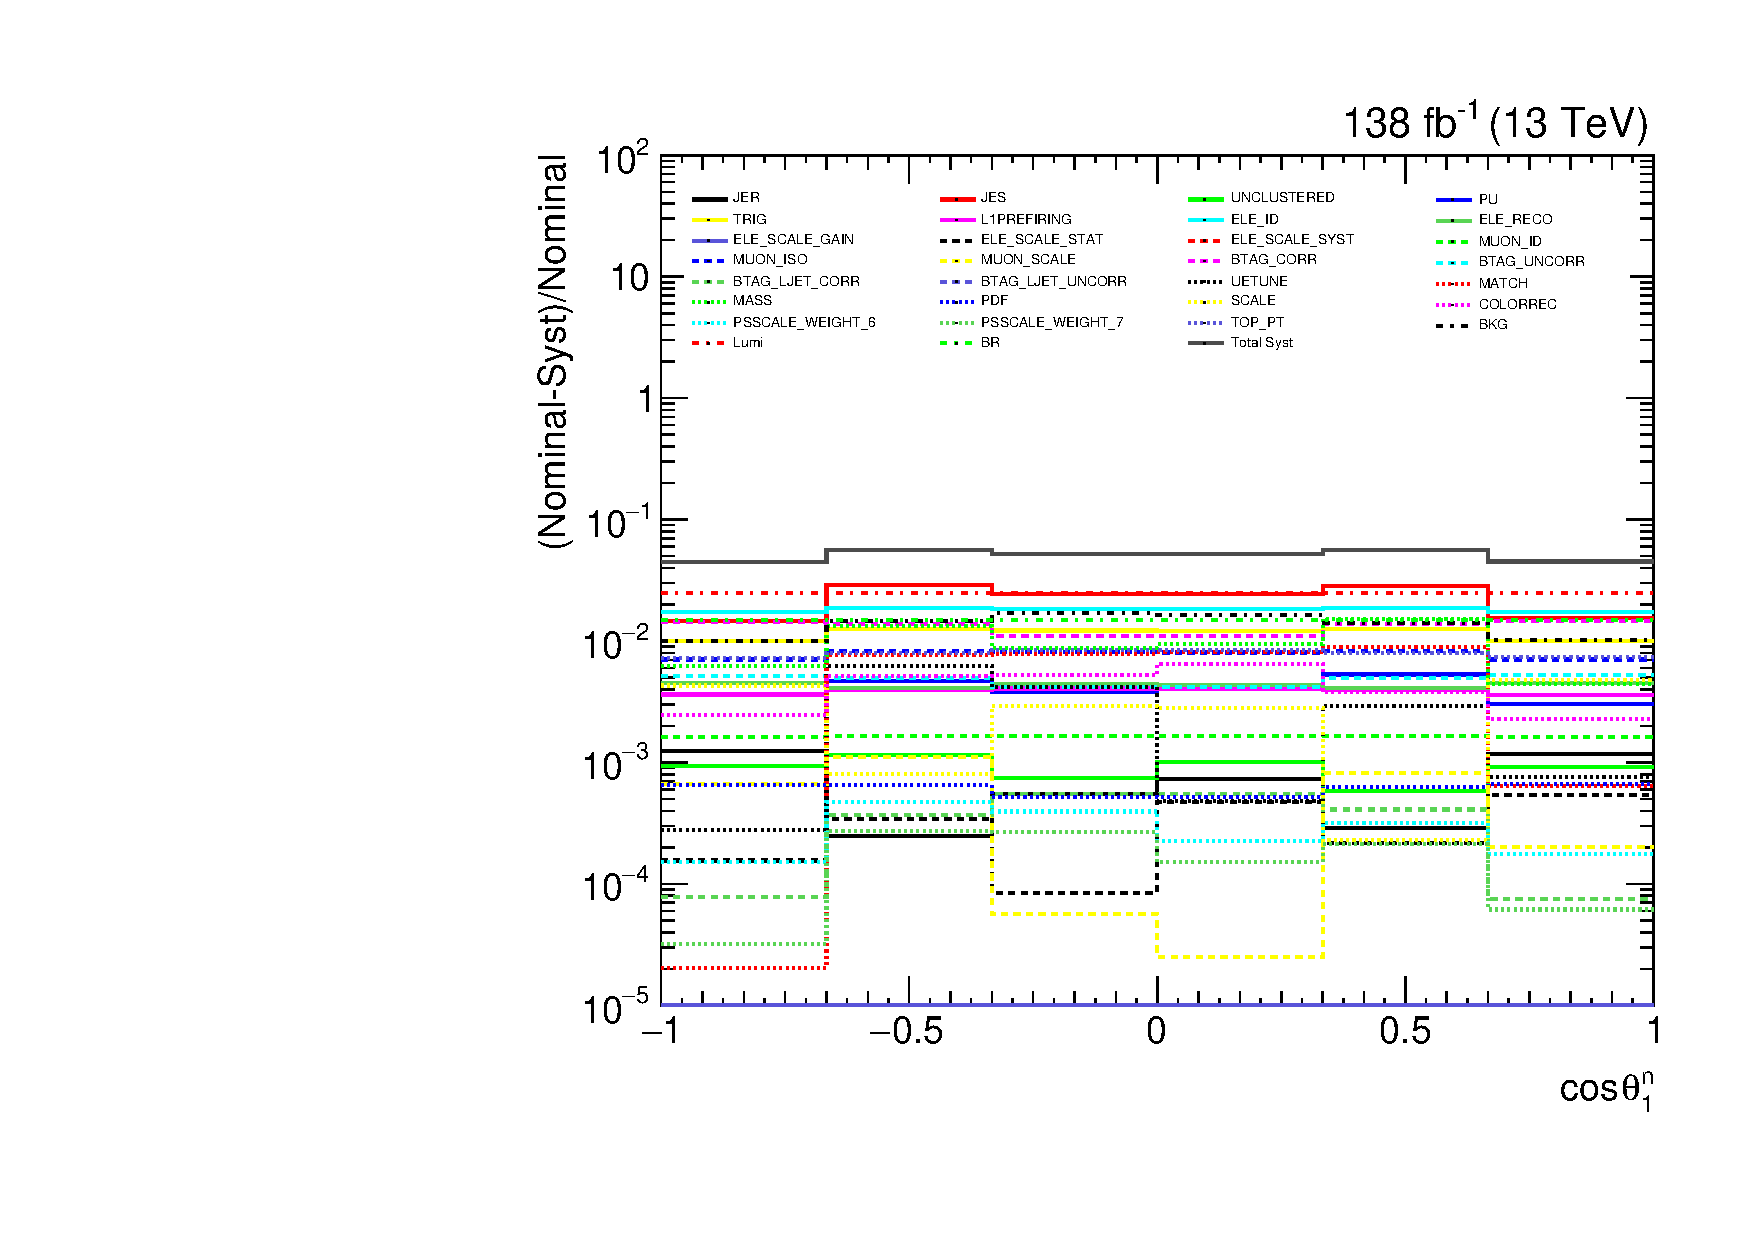
\includegraphics[width=0.32\textwidth]{fig_fullRun2UL/unfolding/combined/deltaSystCombinedlog_rebinnedB_b1n.pdf}
 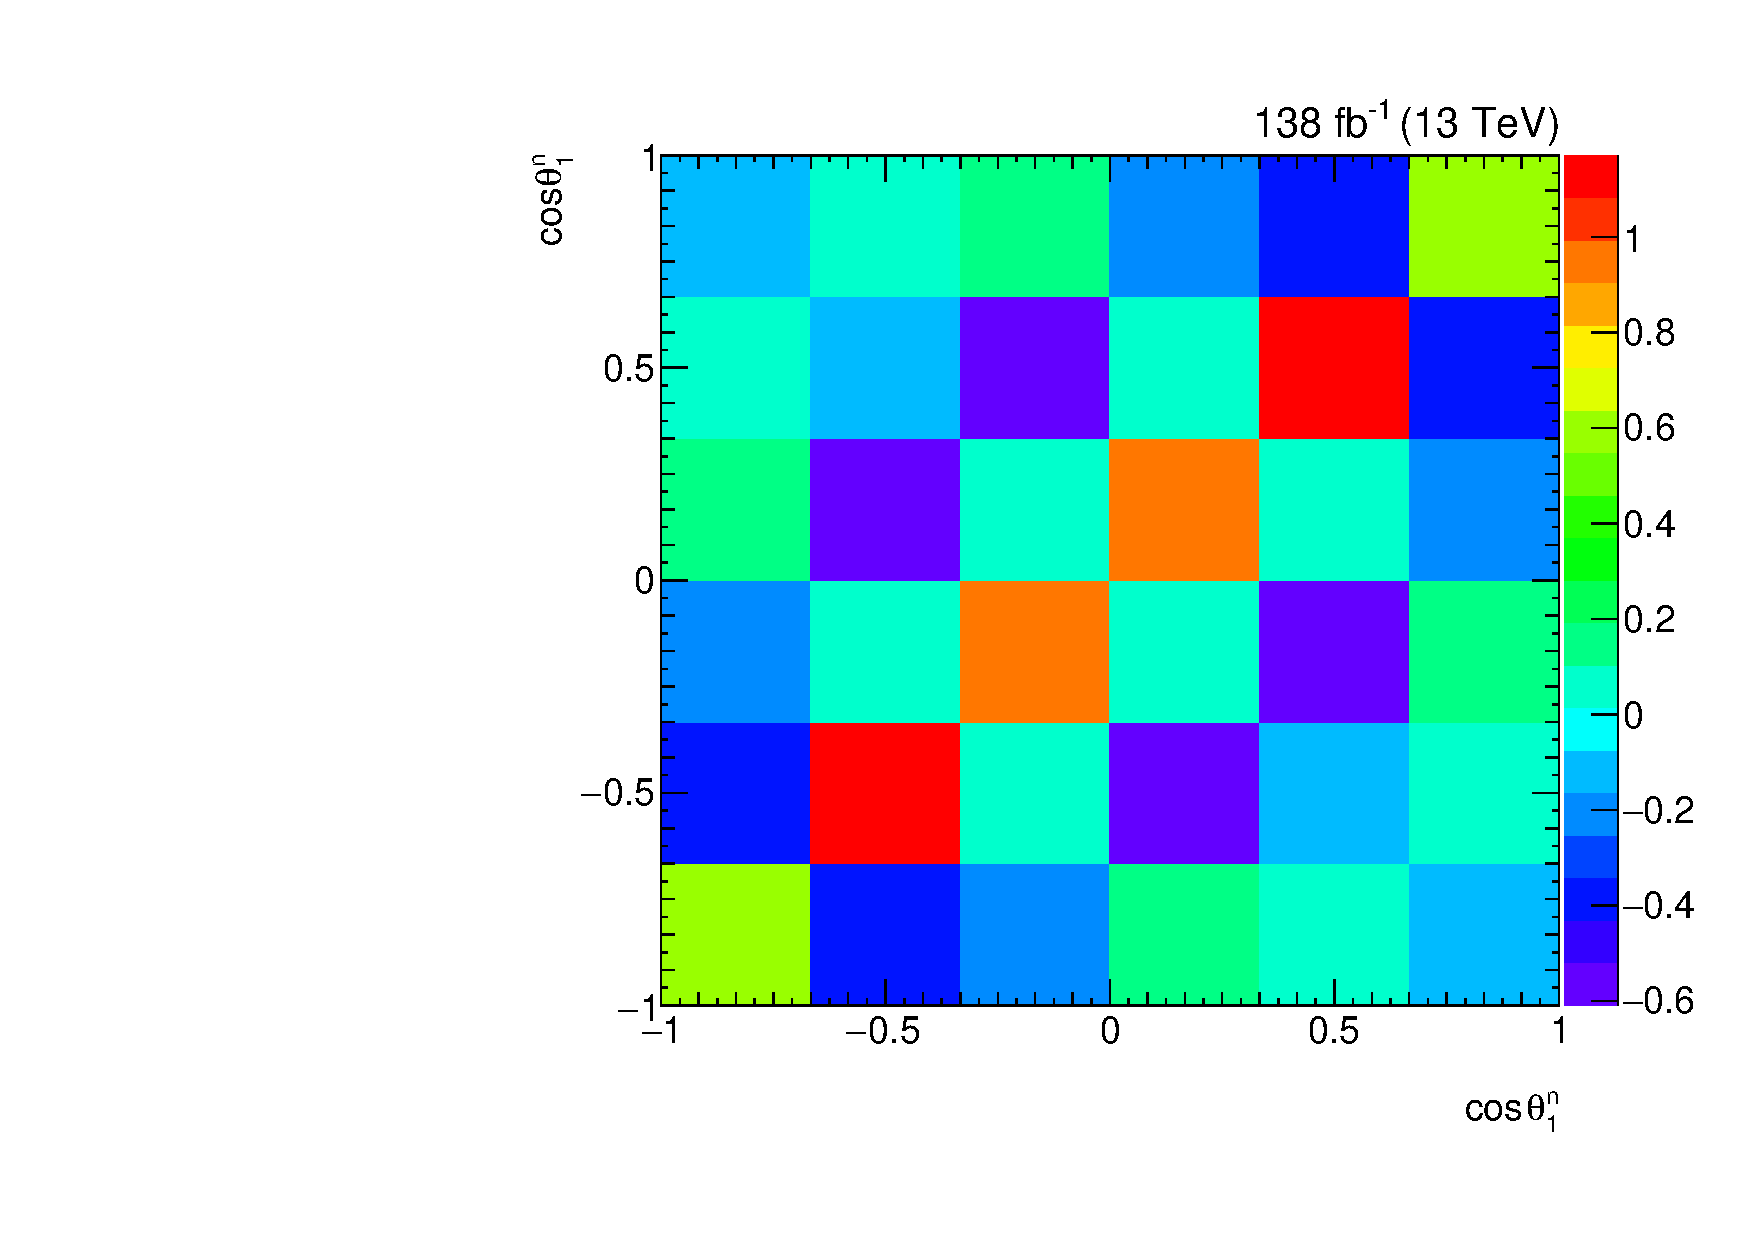
\includegraphics[width=0.32\textwidth]{fig_fullRun2UL/unfolding/combined/StatCovMatrix_rebinnedB_b1n.pdf}
 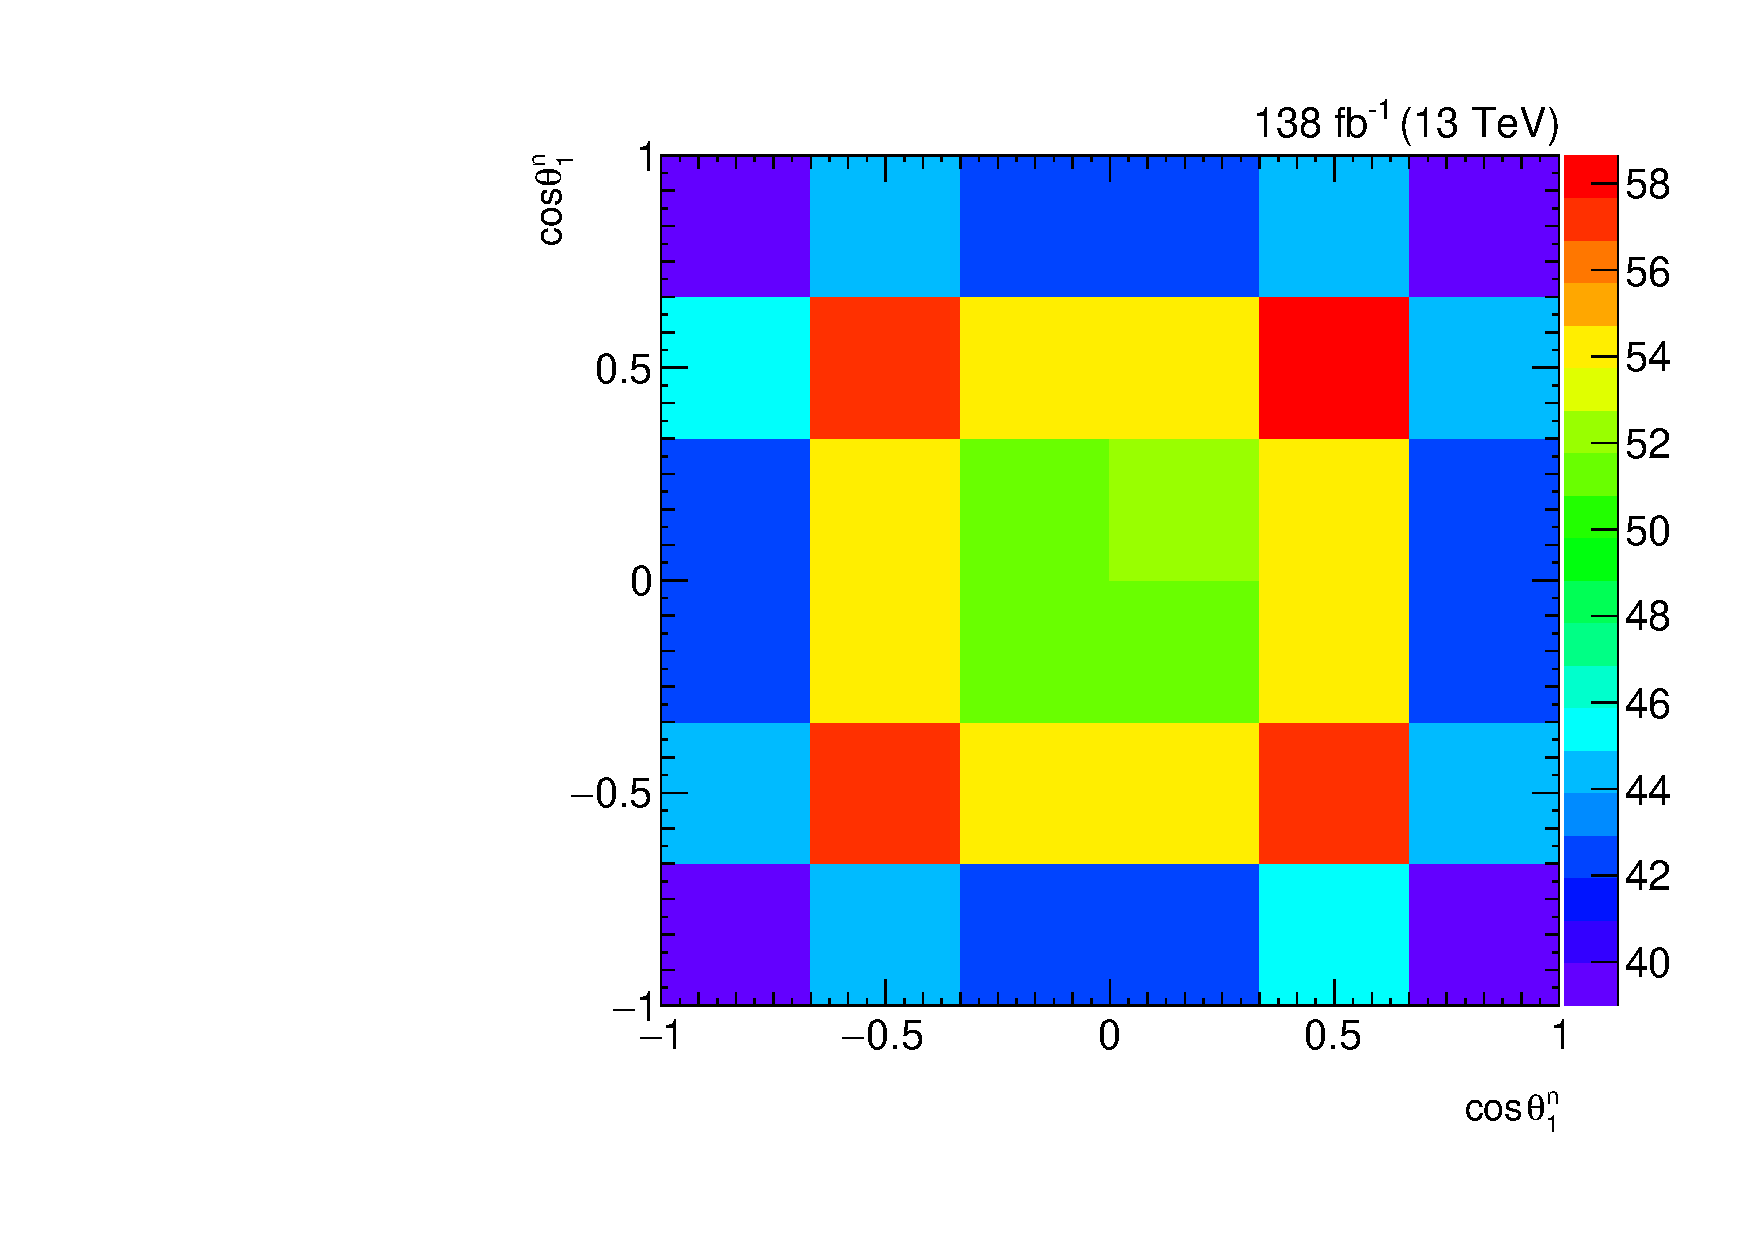
\includegraphics[width=0.32\textwidth]{fig_fullRun2UL/unfolding/combined/TotalSystCovMatrix_rebinnedB_b1n.pdf} \\
 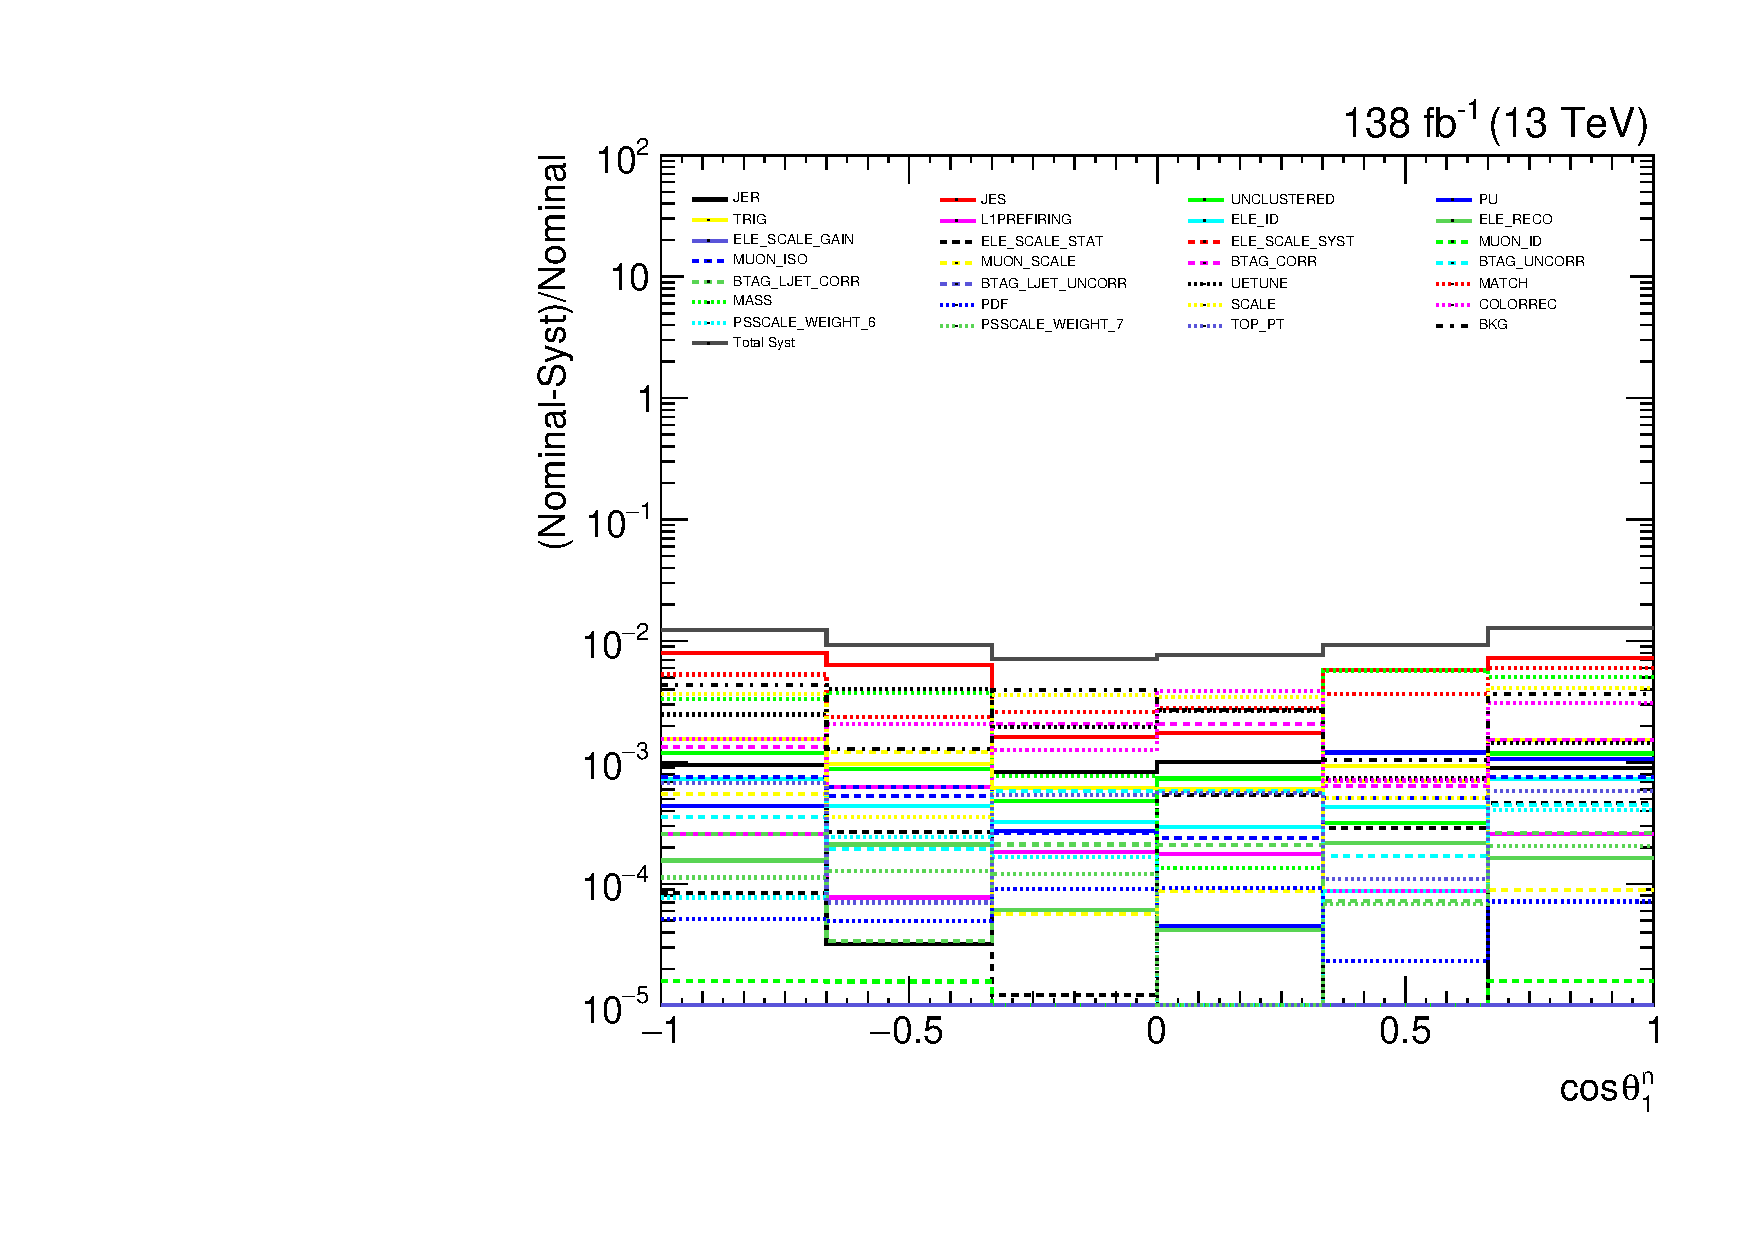
\includegraphics[width=0.32\textwidth]{fig_fullRun2UL/unfolding/combined/deltaSystCombinedlogNorm_rebinnedB_b1n.pdf}
 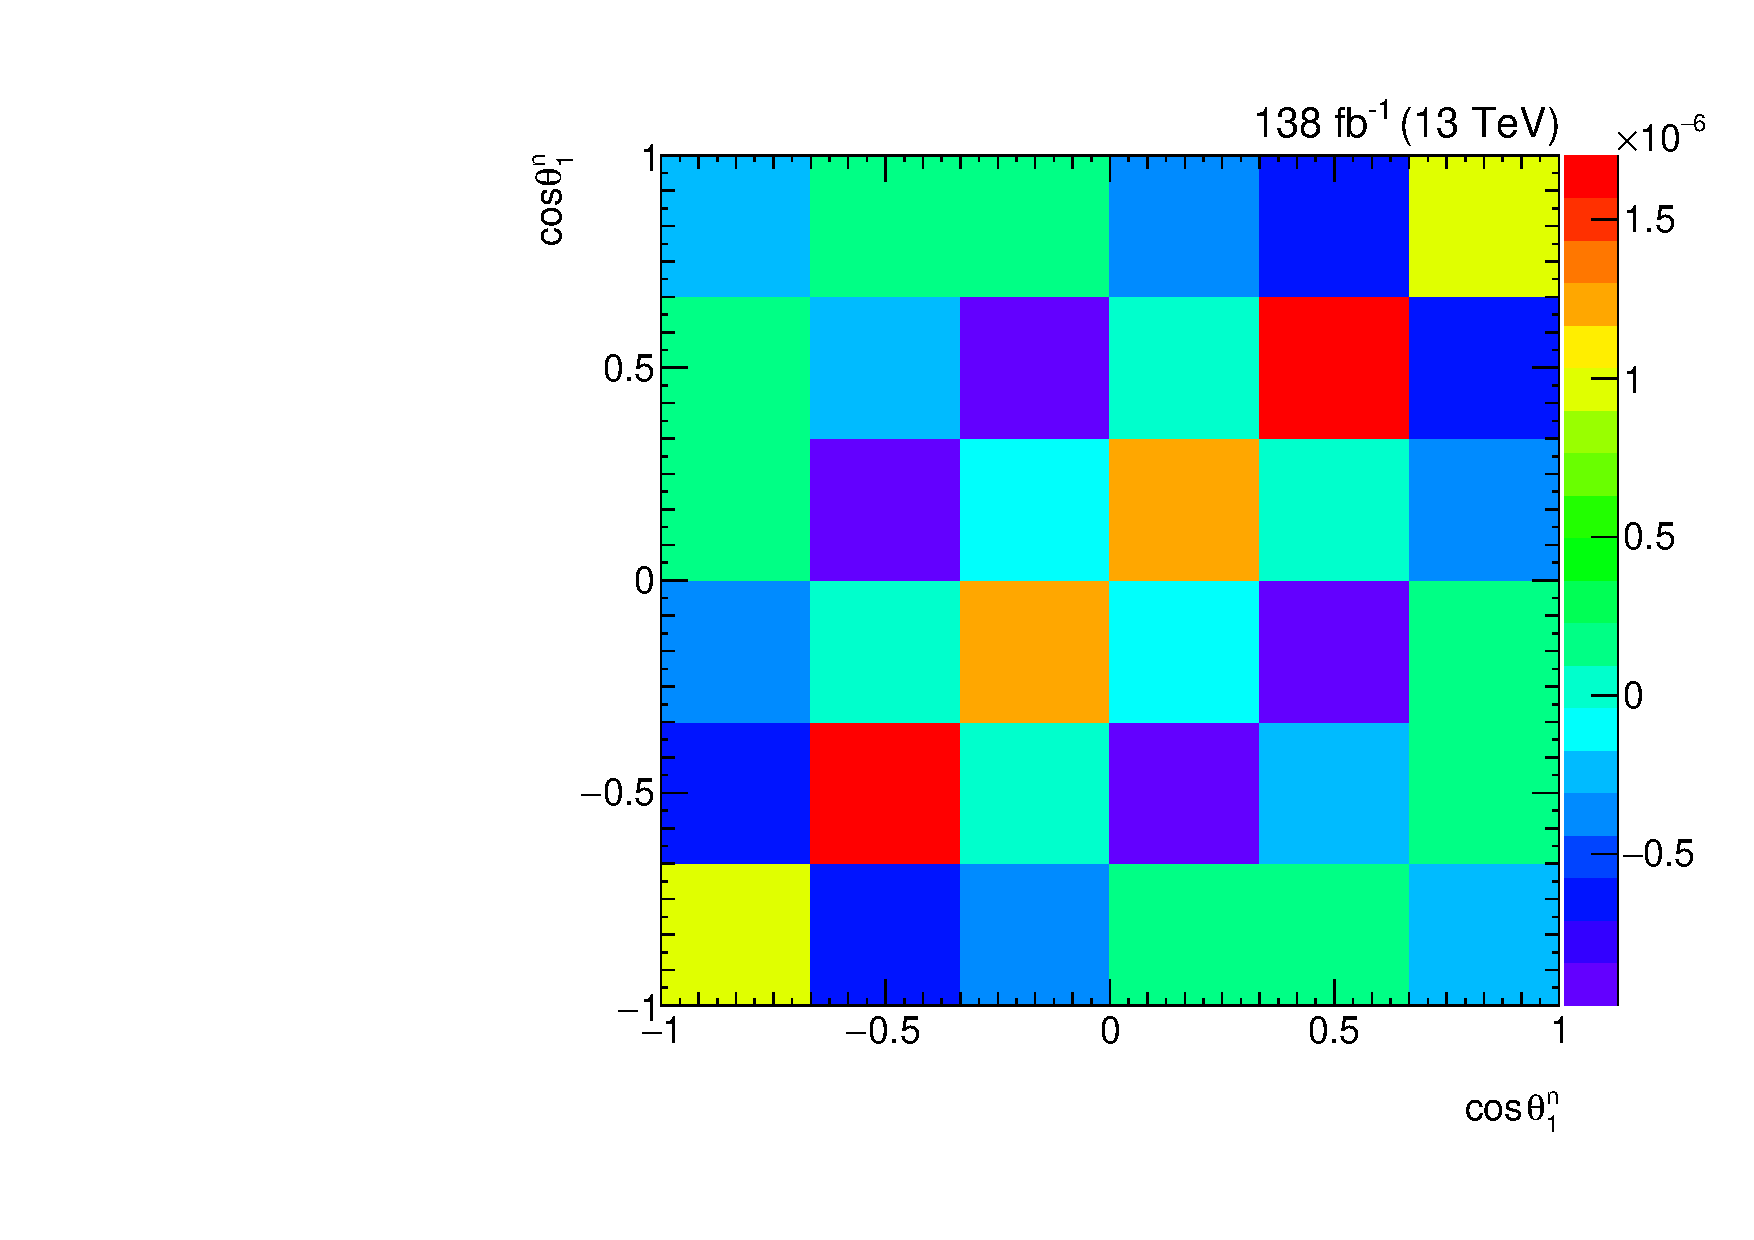
\includegraphics[width=0.32\textwidth]{fig_fullRun2UL/unfolding/combined/StatCovMatrixNorm_rebinnedB_b1n.pdf}
 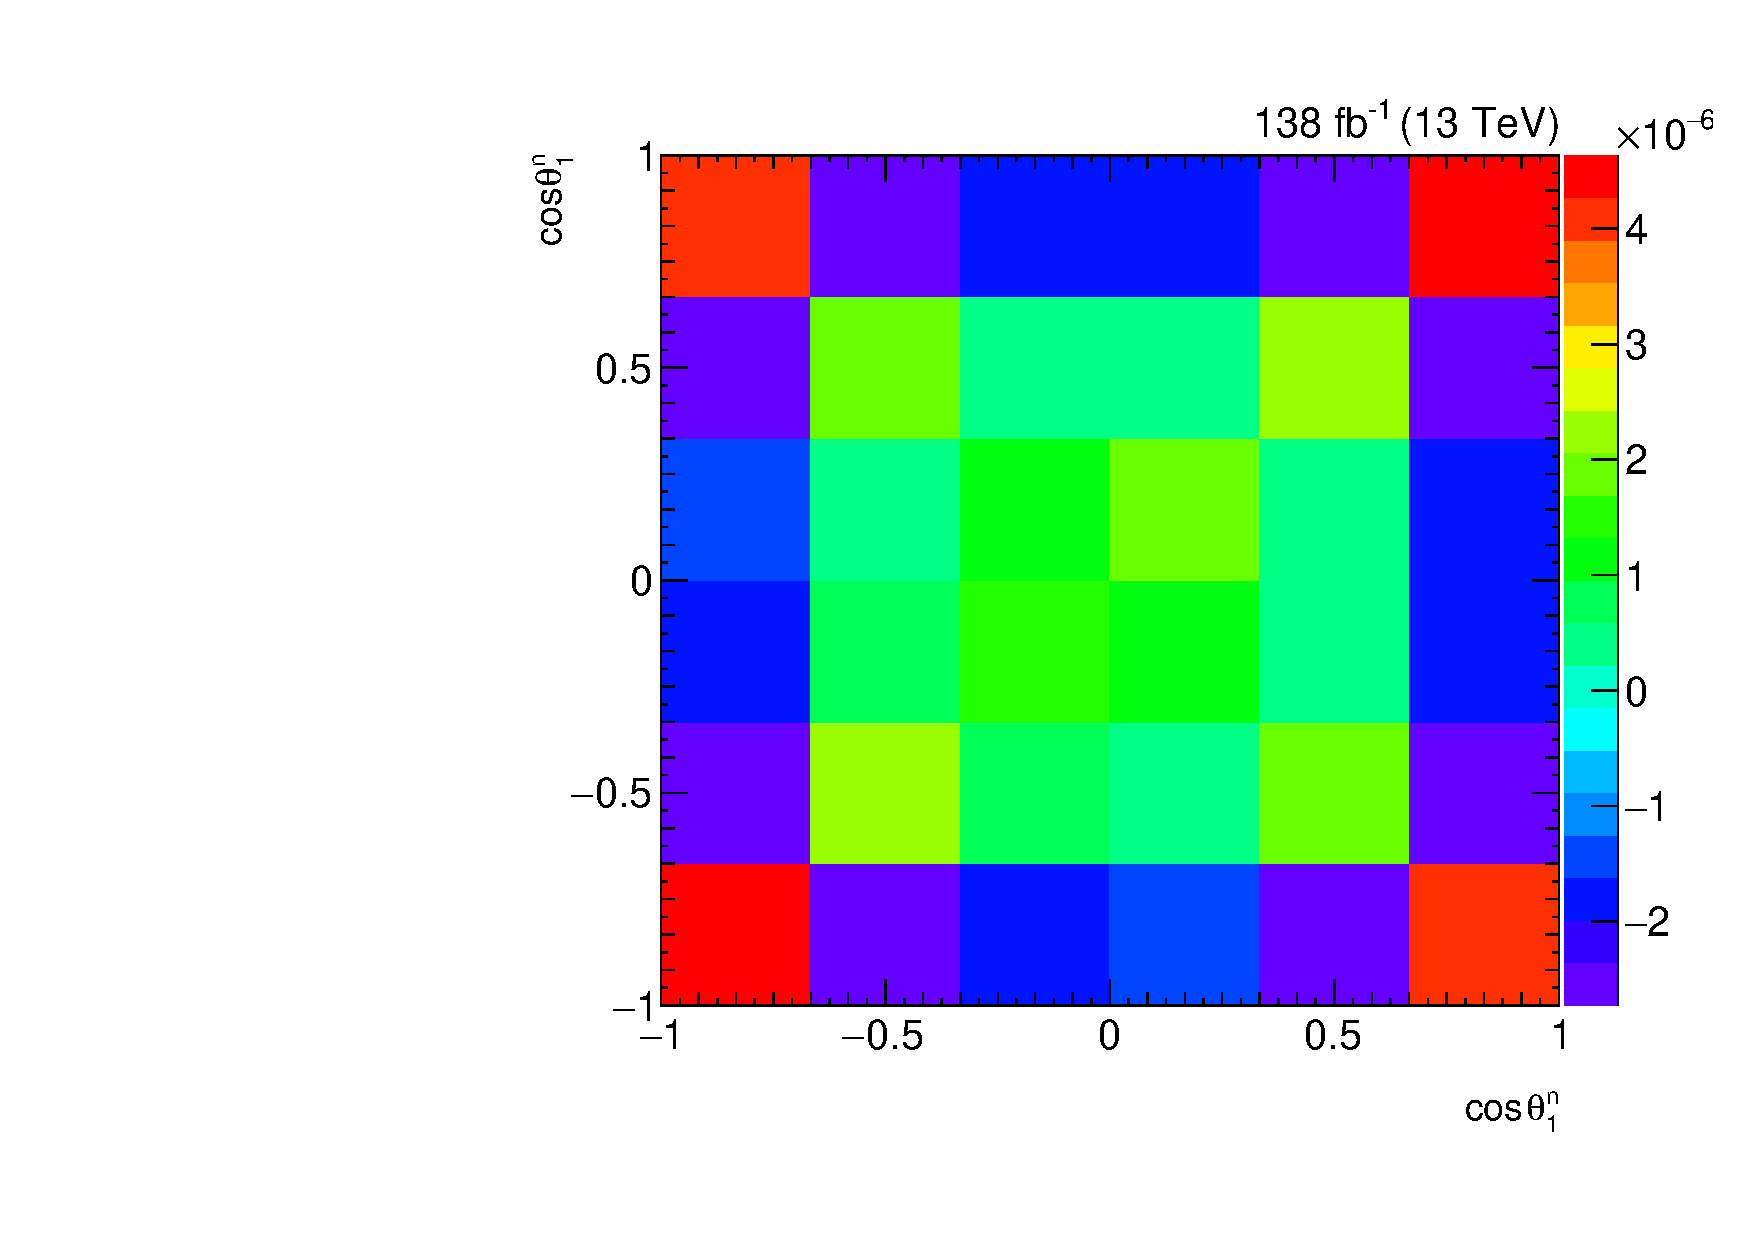
\includegraphics[width=0.32\textwidth]{fig_fullRun2UL/unfolding/combined/TotalSystCovMatrixNorm_rebinnedB_b1n.pdf} \\
\caption{Unfolded-cross section breakdown of uncertainties (Top Left), unfolded cross-section statistical covariance matrix (Top Middle), unfolded cross-section total systematic covariance matrix (Top Right), normalized unfolded-cross section breakdown of uncertainties (Bottom Left), normalized unfolded cross-section statistical covariance matrix (Bottom Middle), normalized unfolded cross-section total systematic covariance matrix (Bottom Right) for polarization observable $\cos\theta_{1}^{n}$.}
\label{fig:b1n_uncertainties}
\end{center}
\end{figure}
\clearpage
\begin{figure}[htb]
\begin{center}
 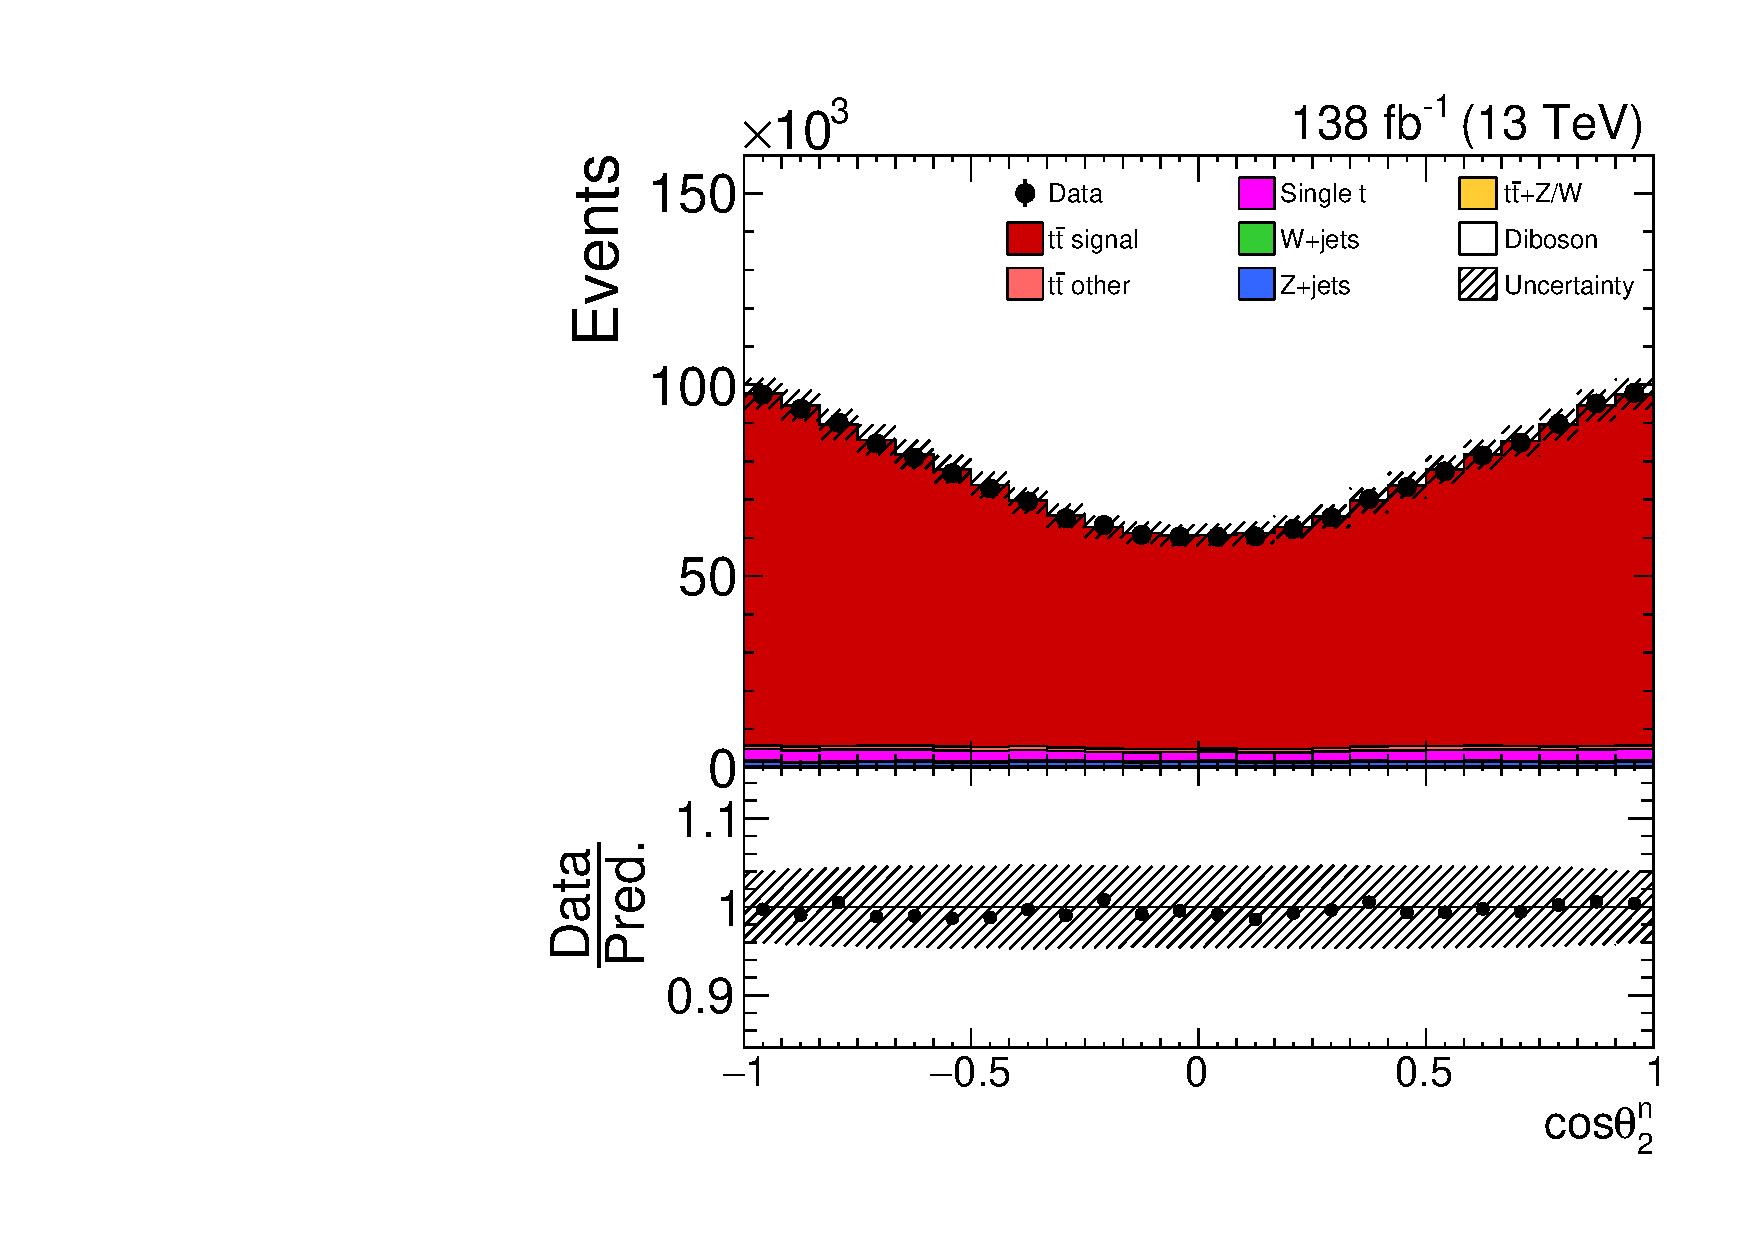
\includegraphics[width=0.32\textwidth]{fig_fullRun2UL/controlplots/combined/Hyp_LeptonBn.pdf}
 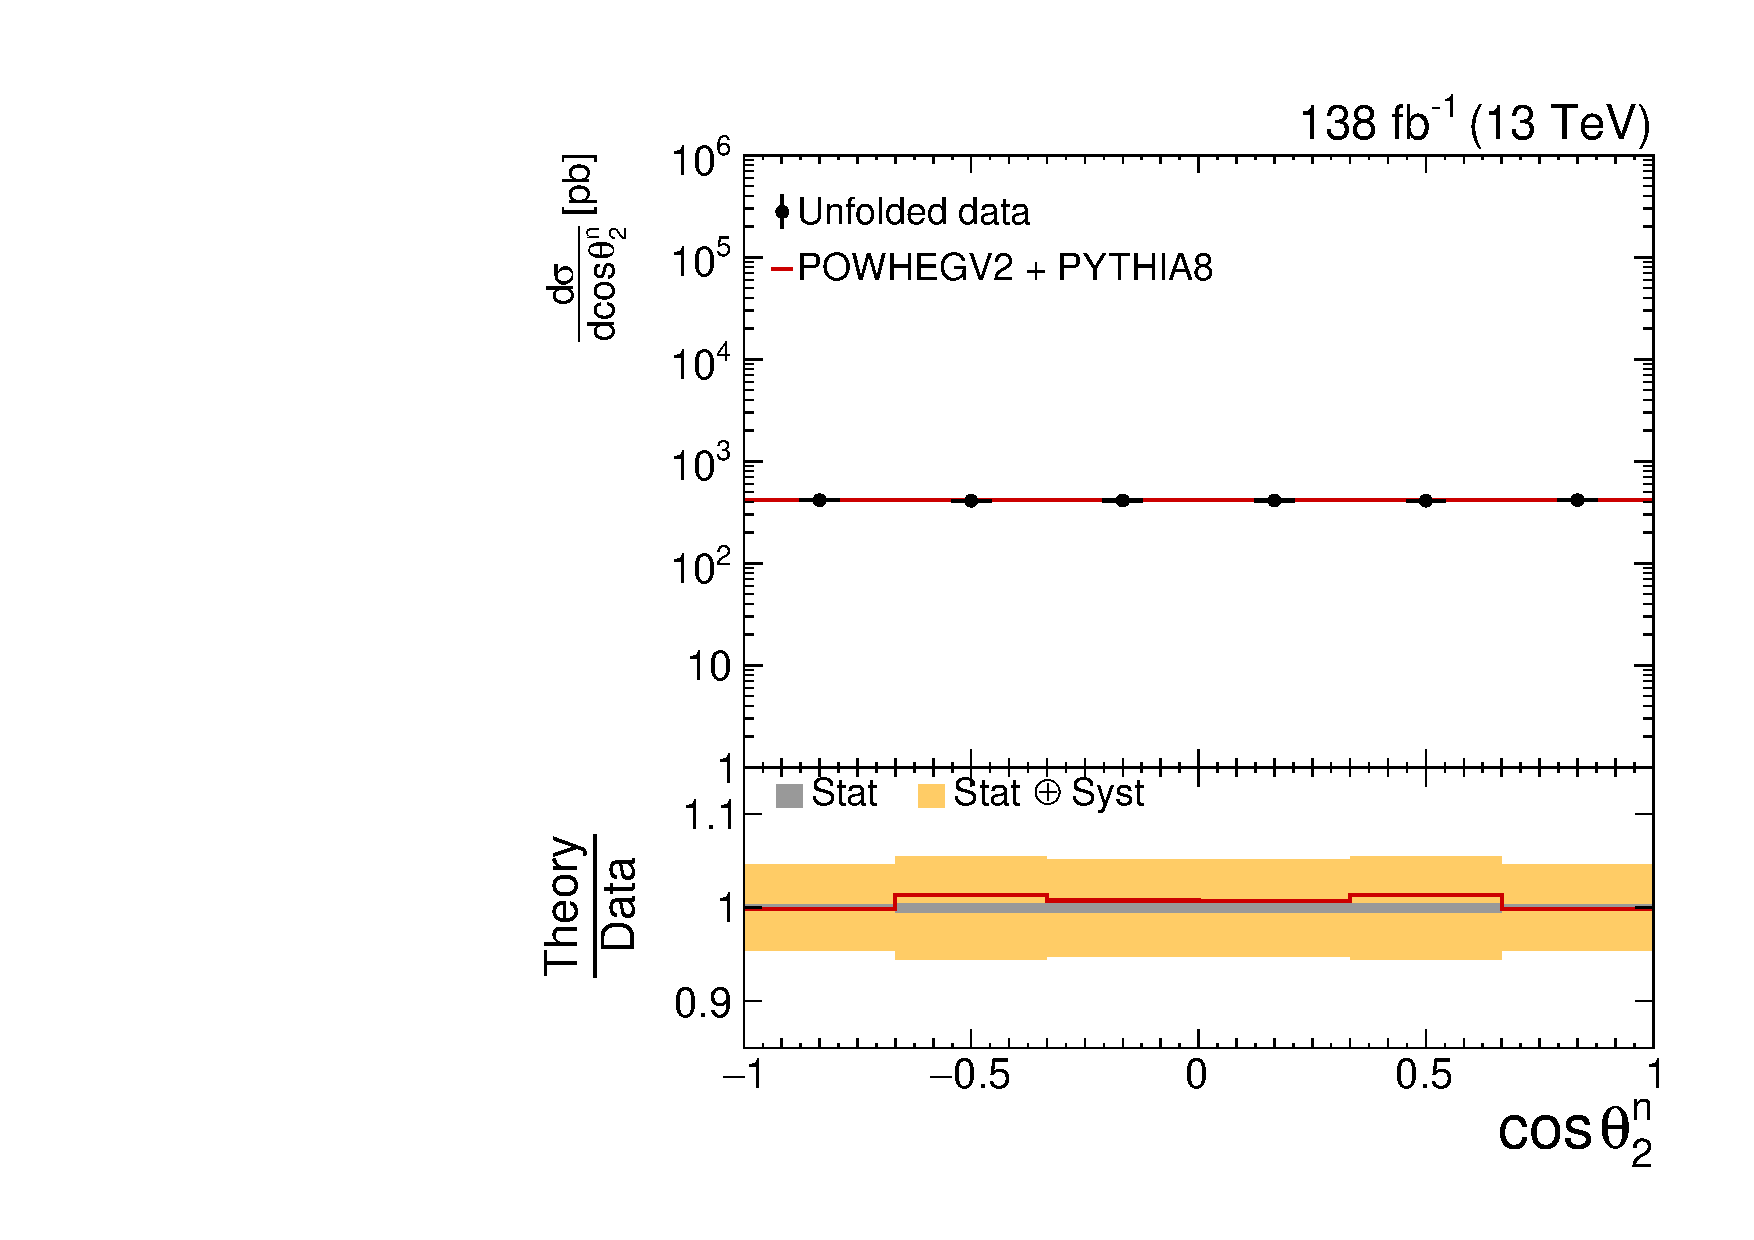
\includegraphics[width=0.32\textwidth]{fig_fullRun2UL/unfolding/combined/UnfoldedResults_b2n.pdf}
 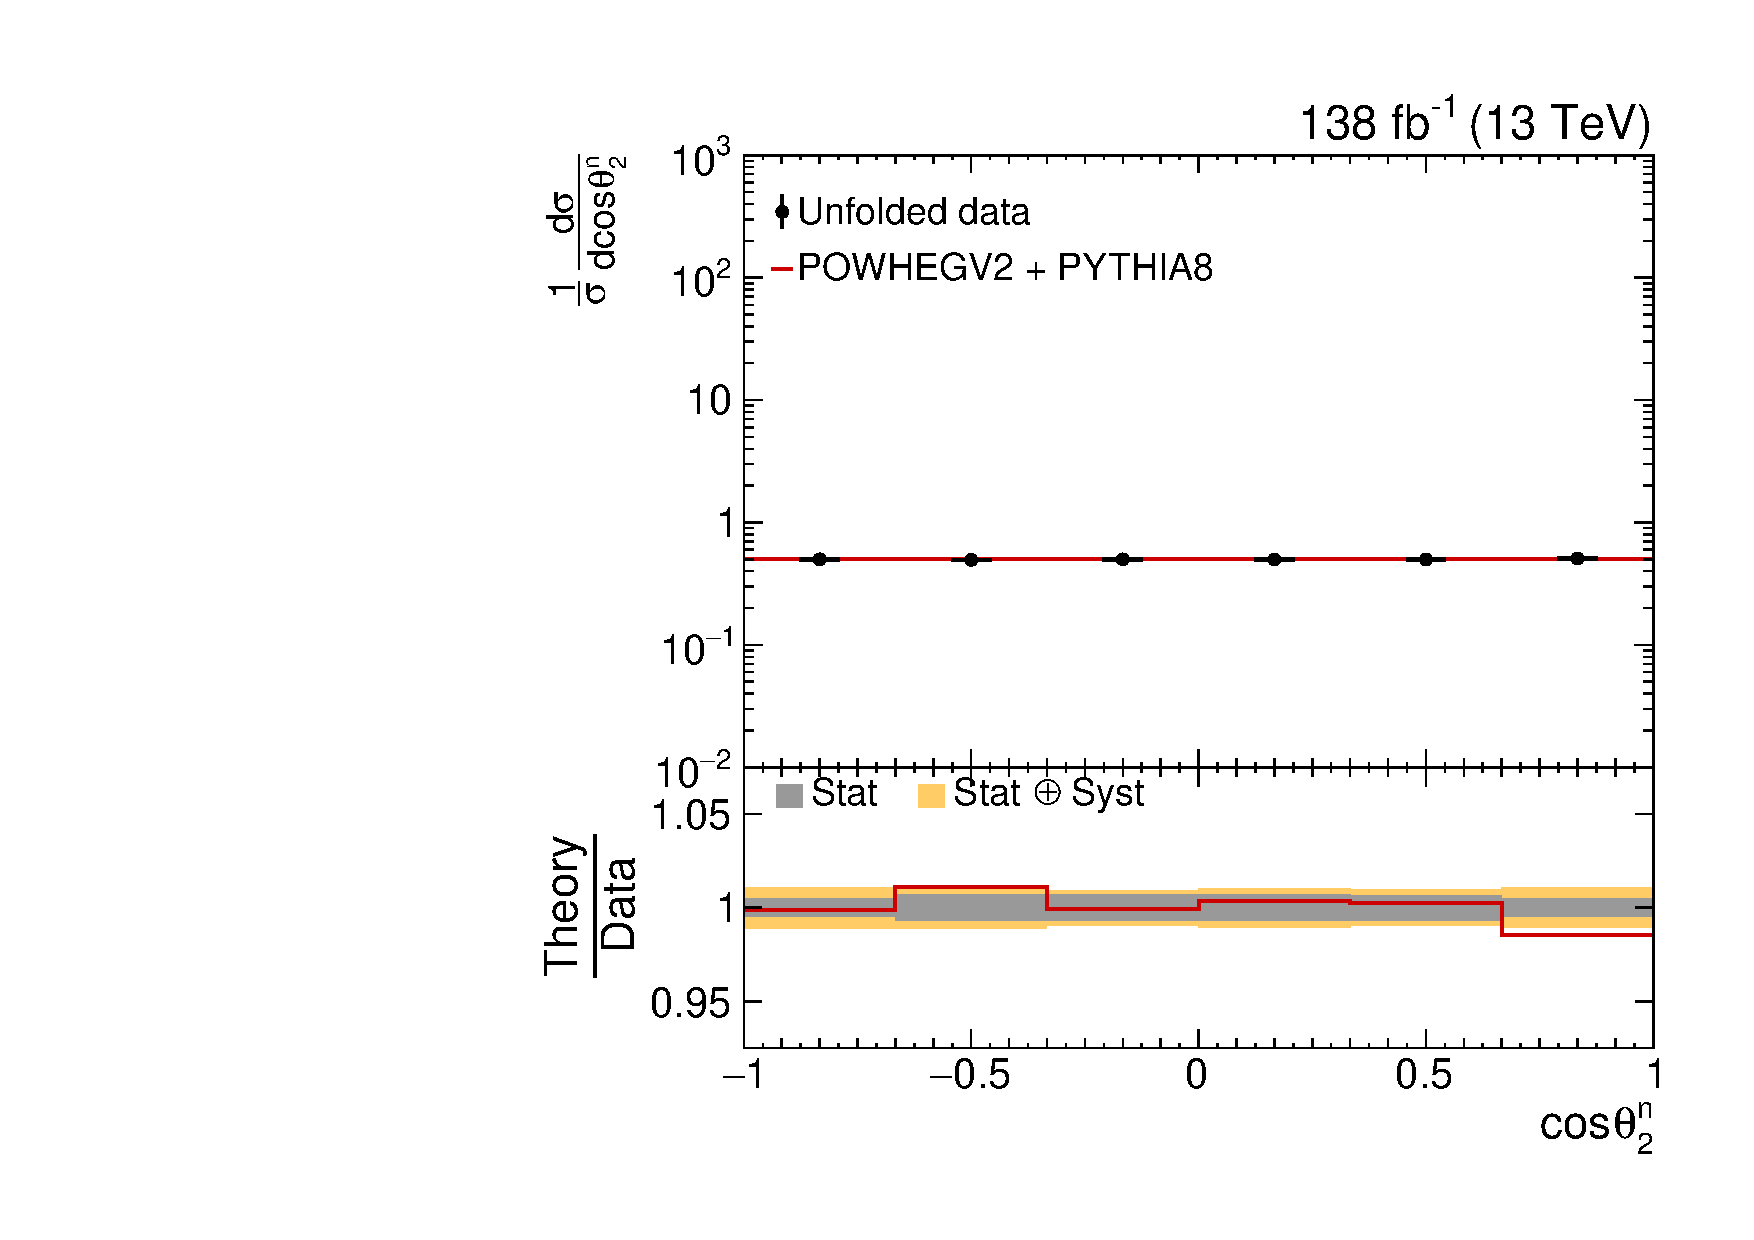
\includegraphics[width=0.32\textwidth]{fig_fullRun2UL/unfolding/combined/UnfoldedResultsNorm_b2n.pdf} \\
 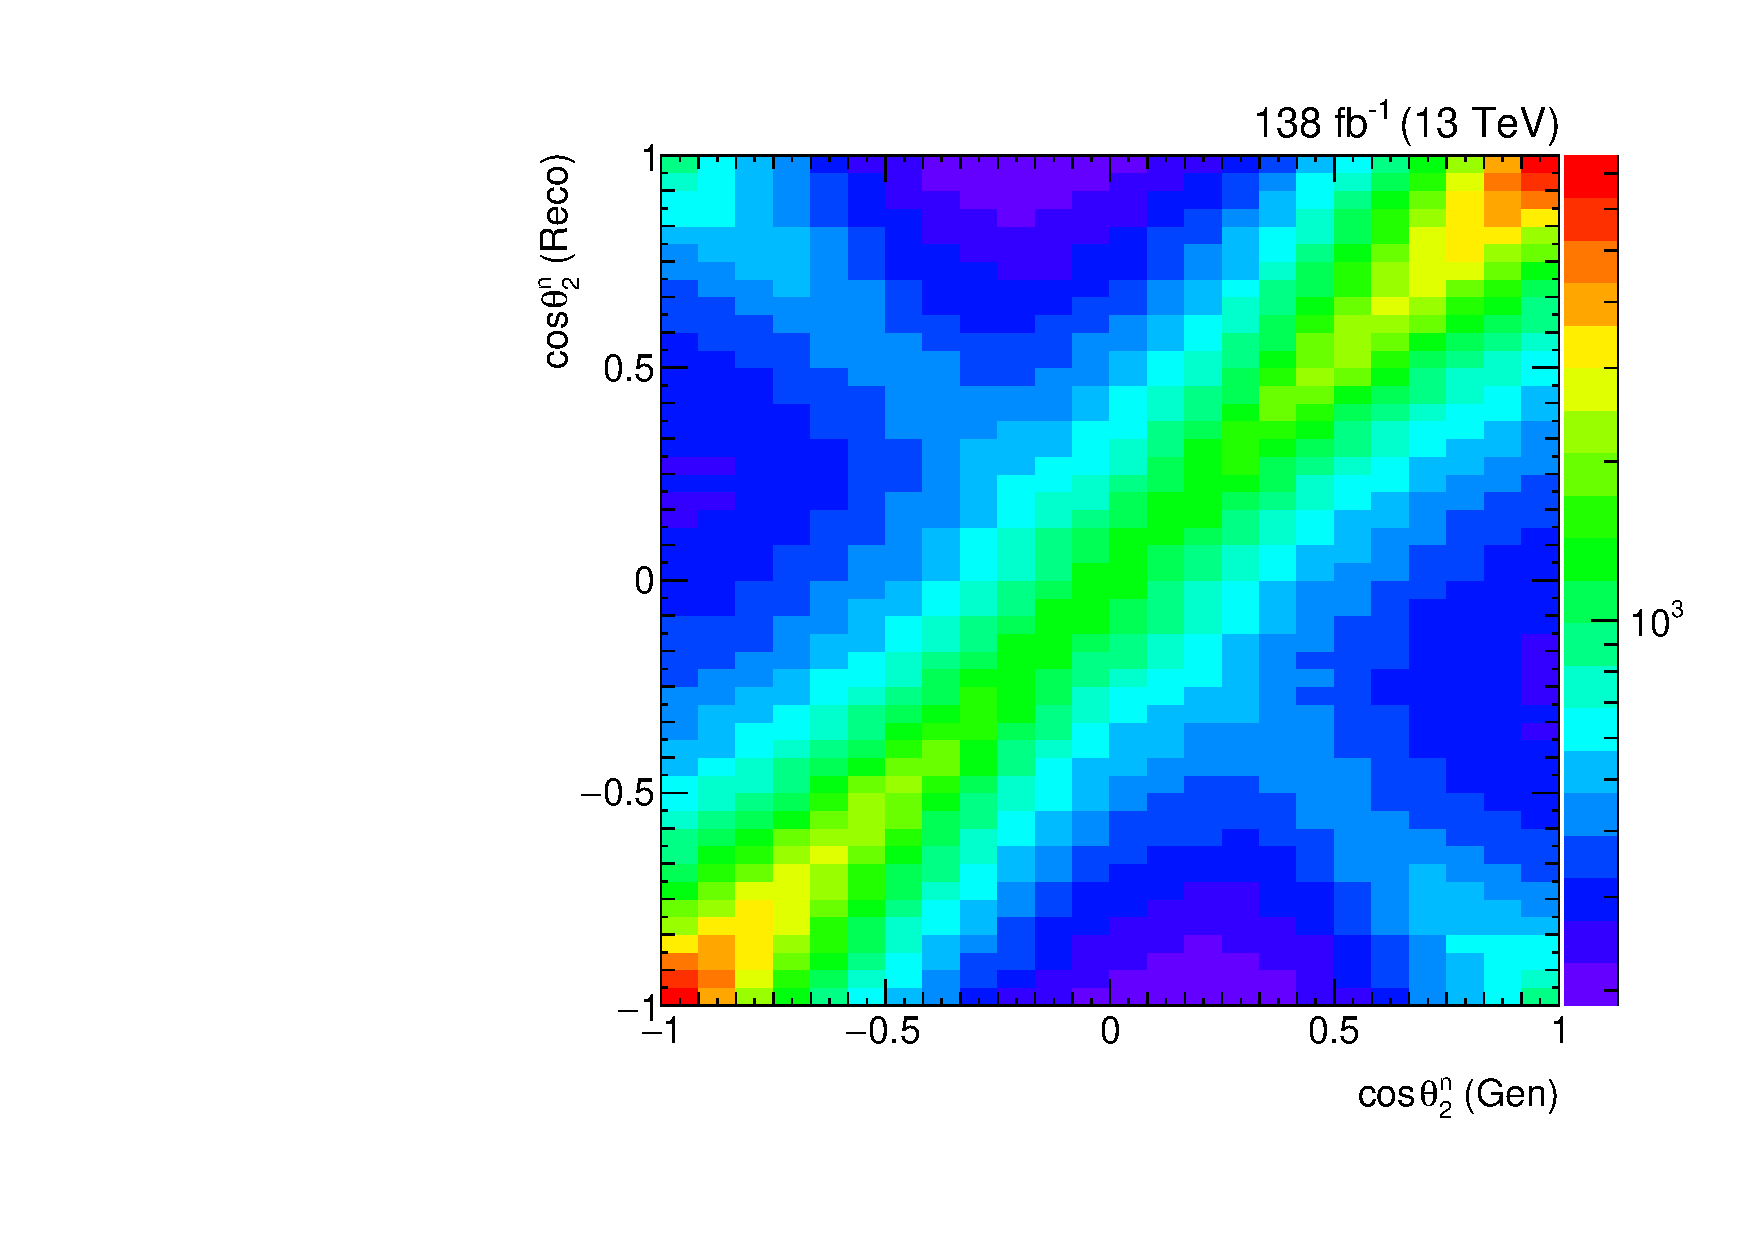
\includegraphics[width=0.32\textwidth]{fig_fullRun2UL/unfolding/combined/ResponseMatrix_b2n.pdf}
 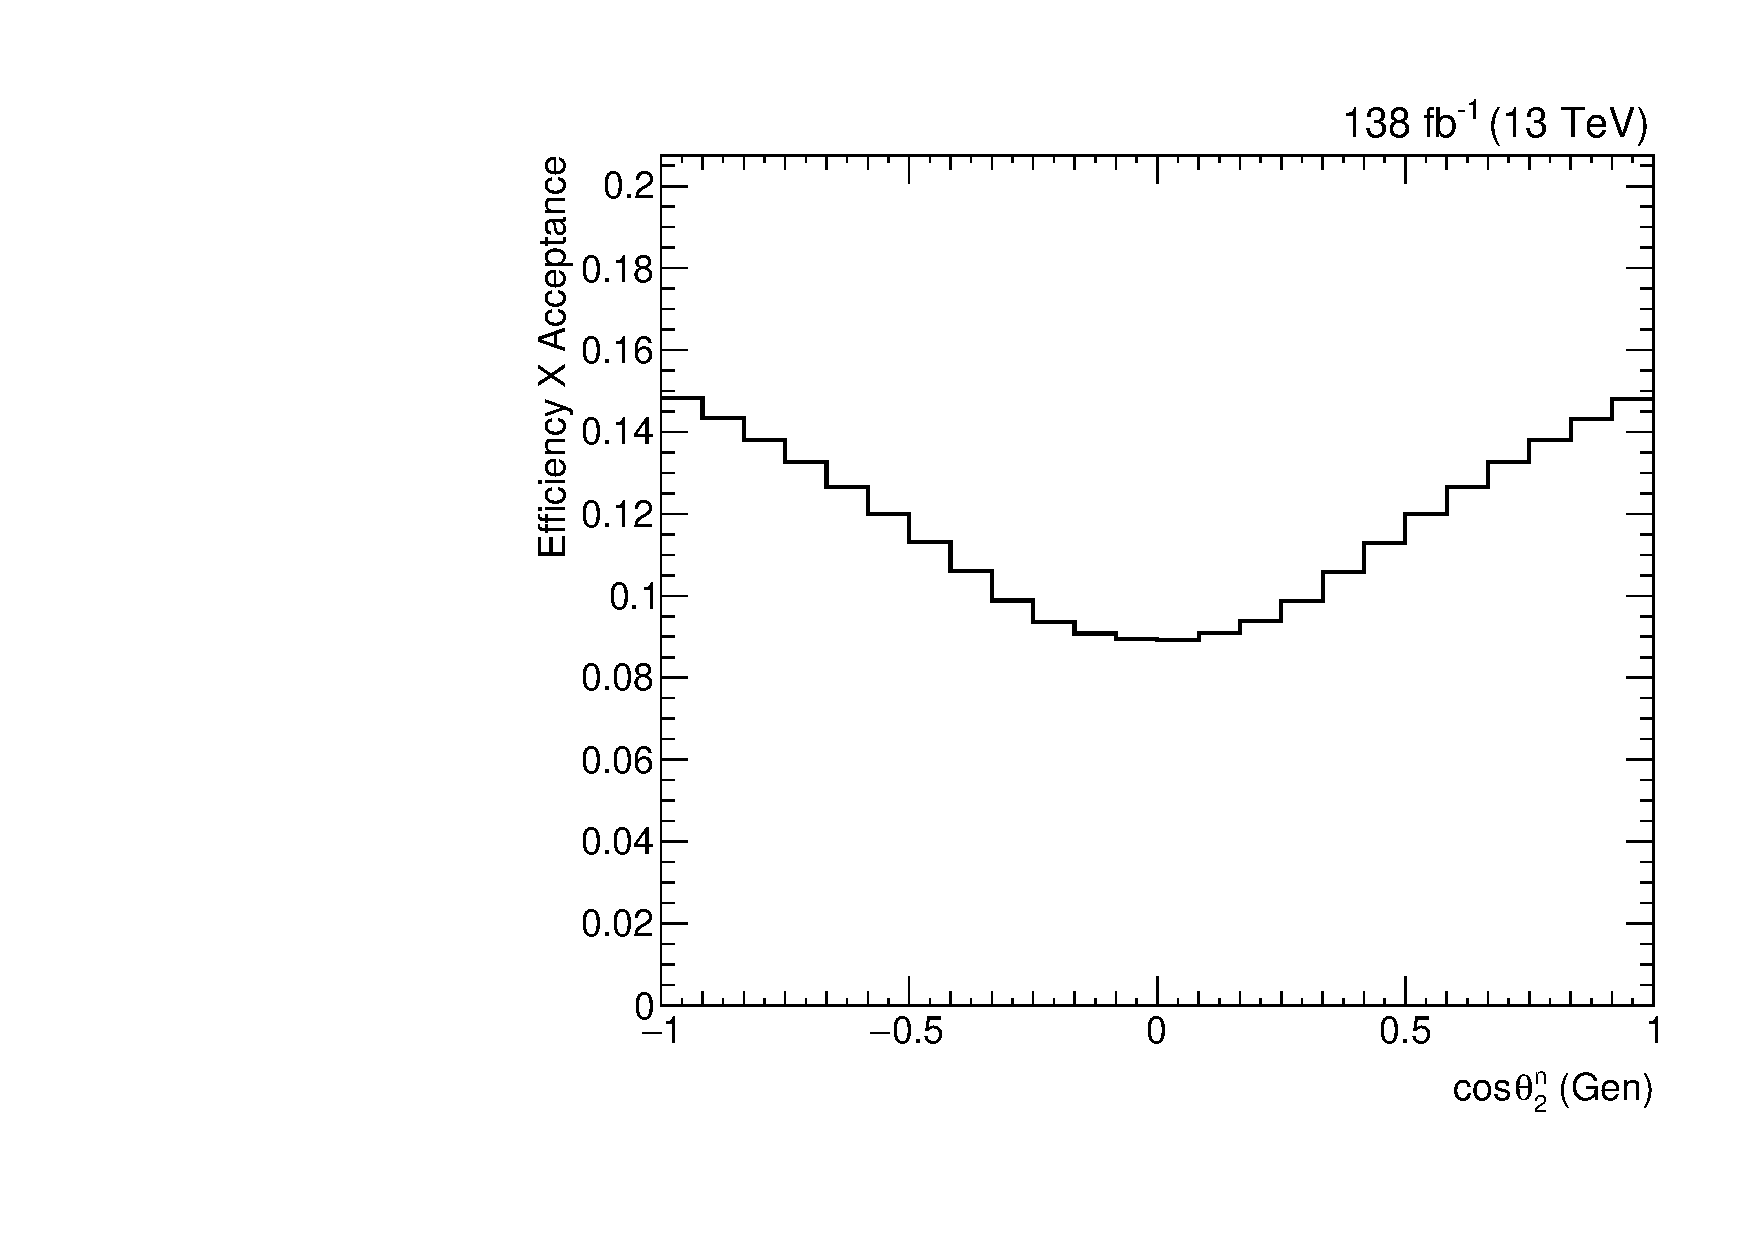
\includegraphics[width=0.32\textwidth]{fig_fullRun2UL/unfolding/combined/TotEff_b2n.pdf}
 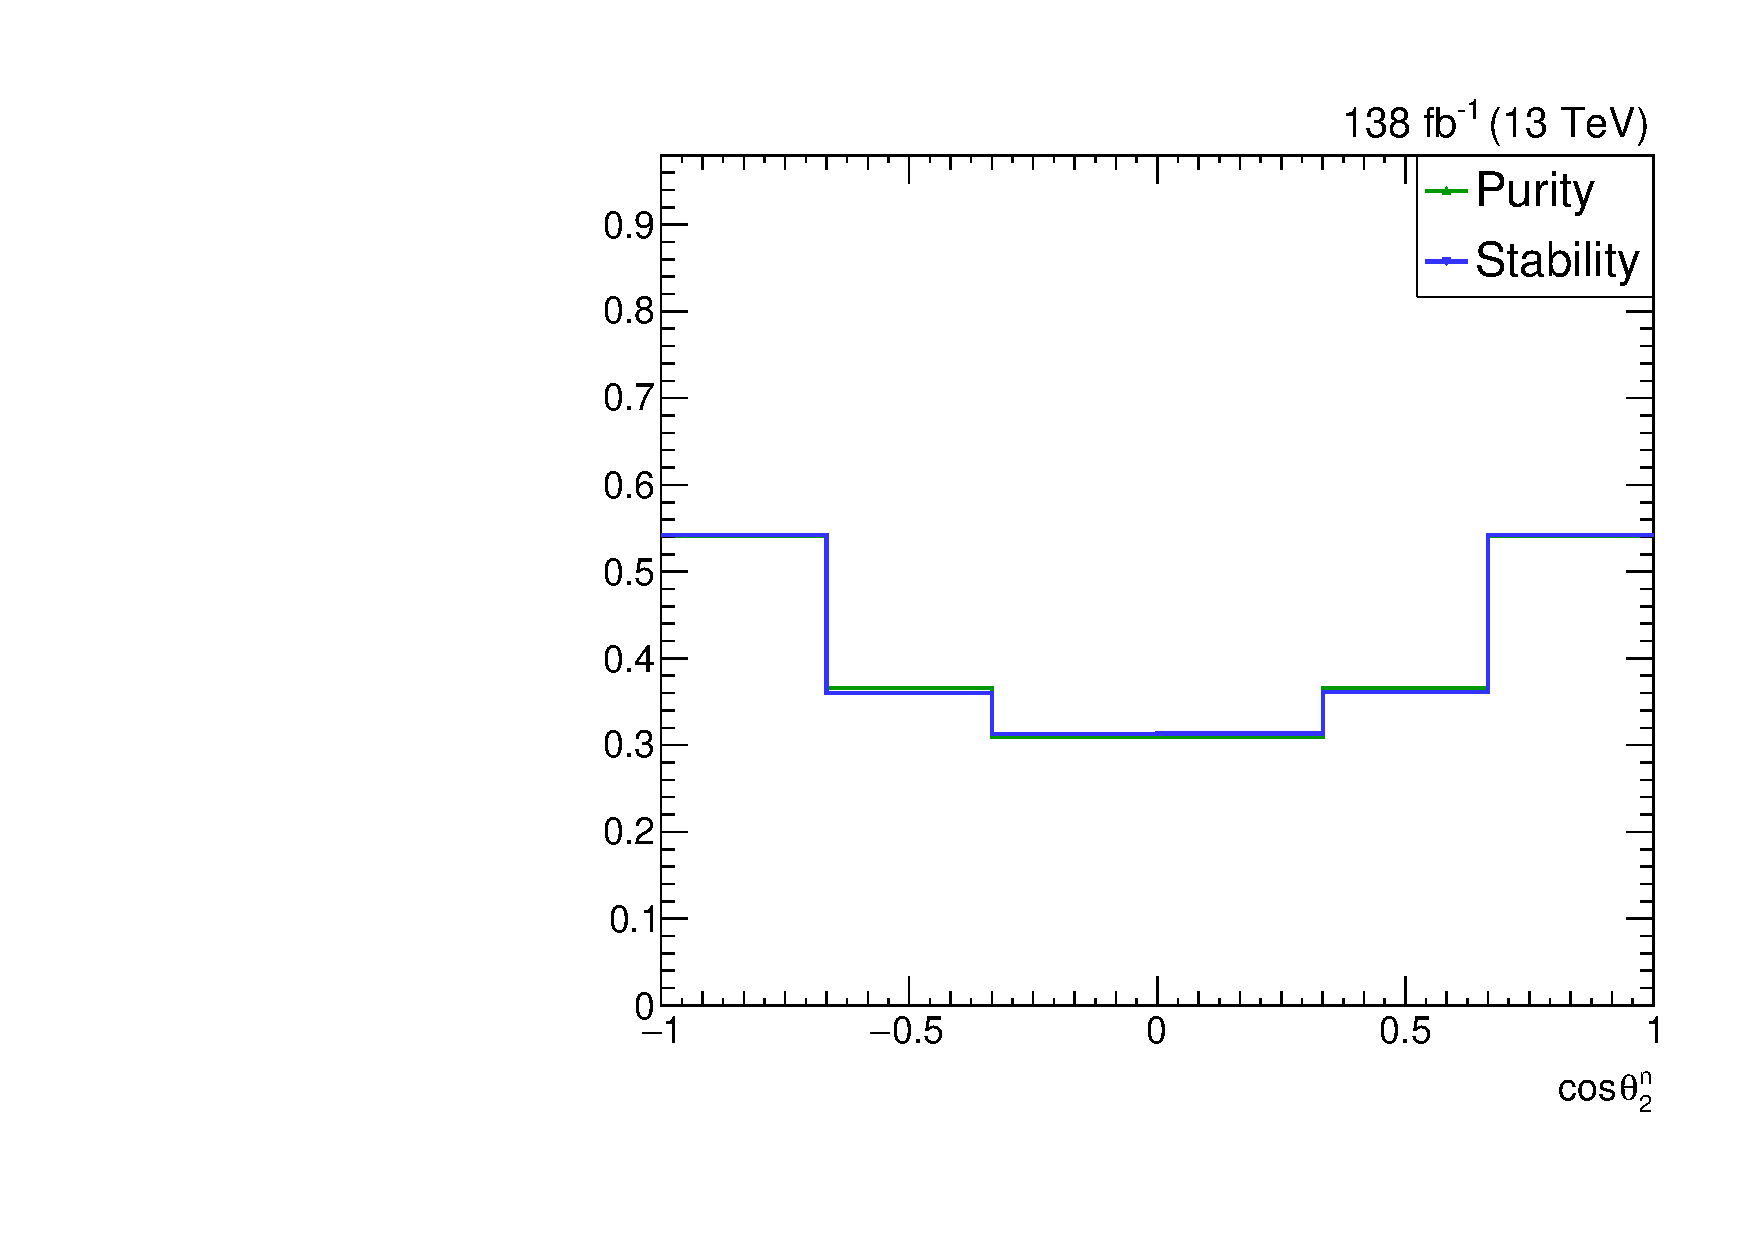
\includegraphics[width=0.32\textwidth]{fig_fullRun2UL/unfolding/combined/PurStab_b2n.pdf} \\
\caption{Reconstructed detector-level distribution (Top Left), absolute cross-section unfolded to parton-level (Top Middle), normalized cross-section unfolded to parton-level (Top Right), detector response-matrix (Bottom Left), efficiency$\times$acceptance (Bottom Middle), Purity and Stability (Bottom Right) for polarization observable $\cos\theta_{2}^{n}$, from which spin-density coefficient $B_{2}^{n}$ (sensitive to spin-density coefficient function $b_n^{-}$) is extracted.}
\label{fig:b2n}
\end{center}
\end{figure}
\clearpage
\begin{figure}[htb]
\begin{center}
 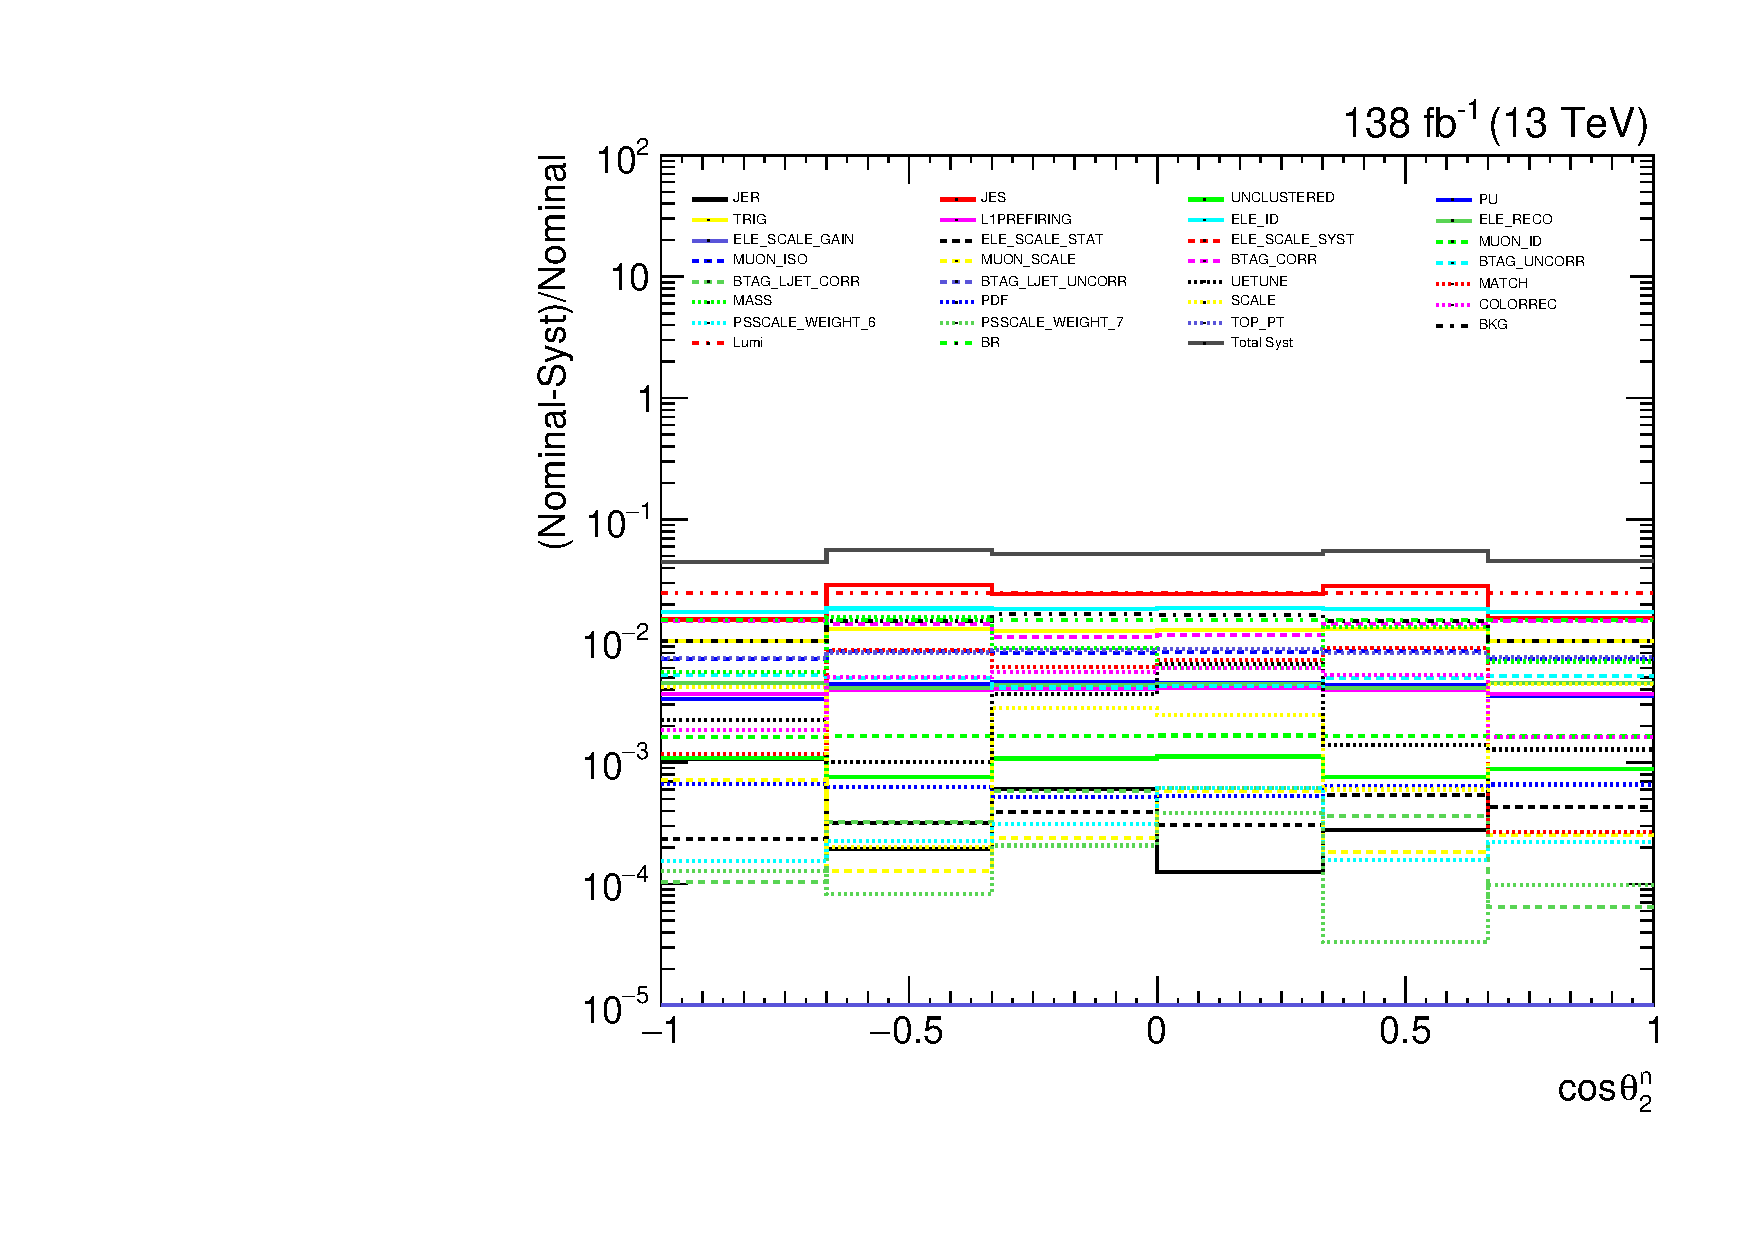
\includegraphics[width=0.32\textwidth]{fig_fullRun2UL/unfolding/combined/deltaSystCombinedlog_rebinnedB_b2n.pdf}
 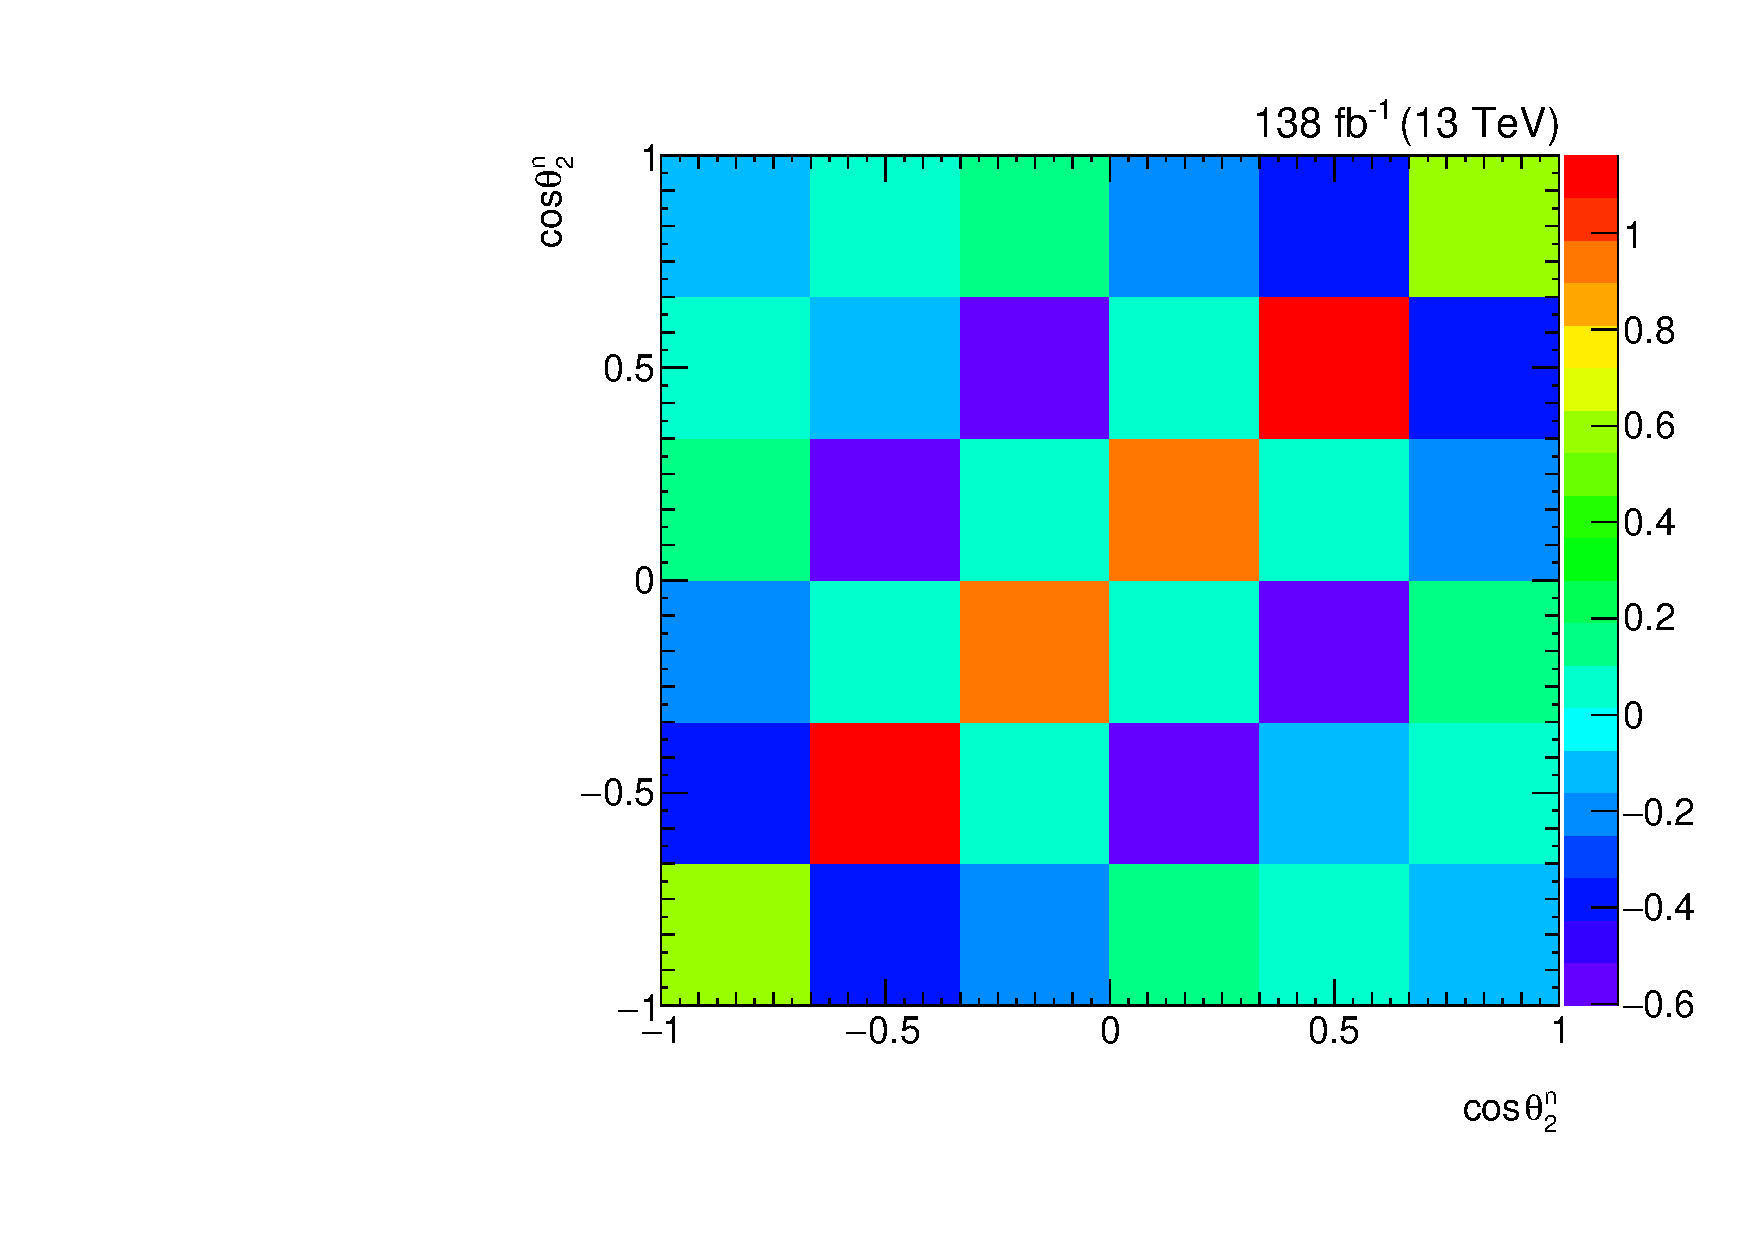
\includegraphics[width=0.32\textwidth]{fig_fullRun2UL/unfolding/combined/StatCovMatrix_rebinnedB_b2n.pdf}
 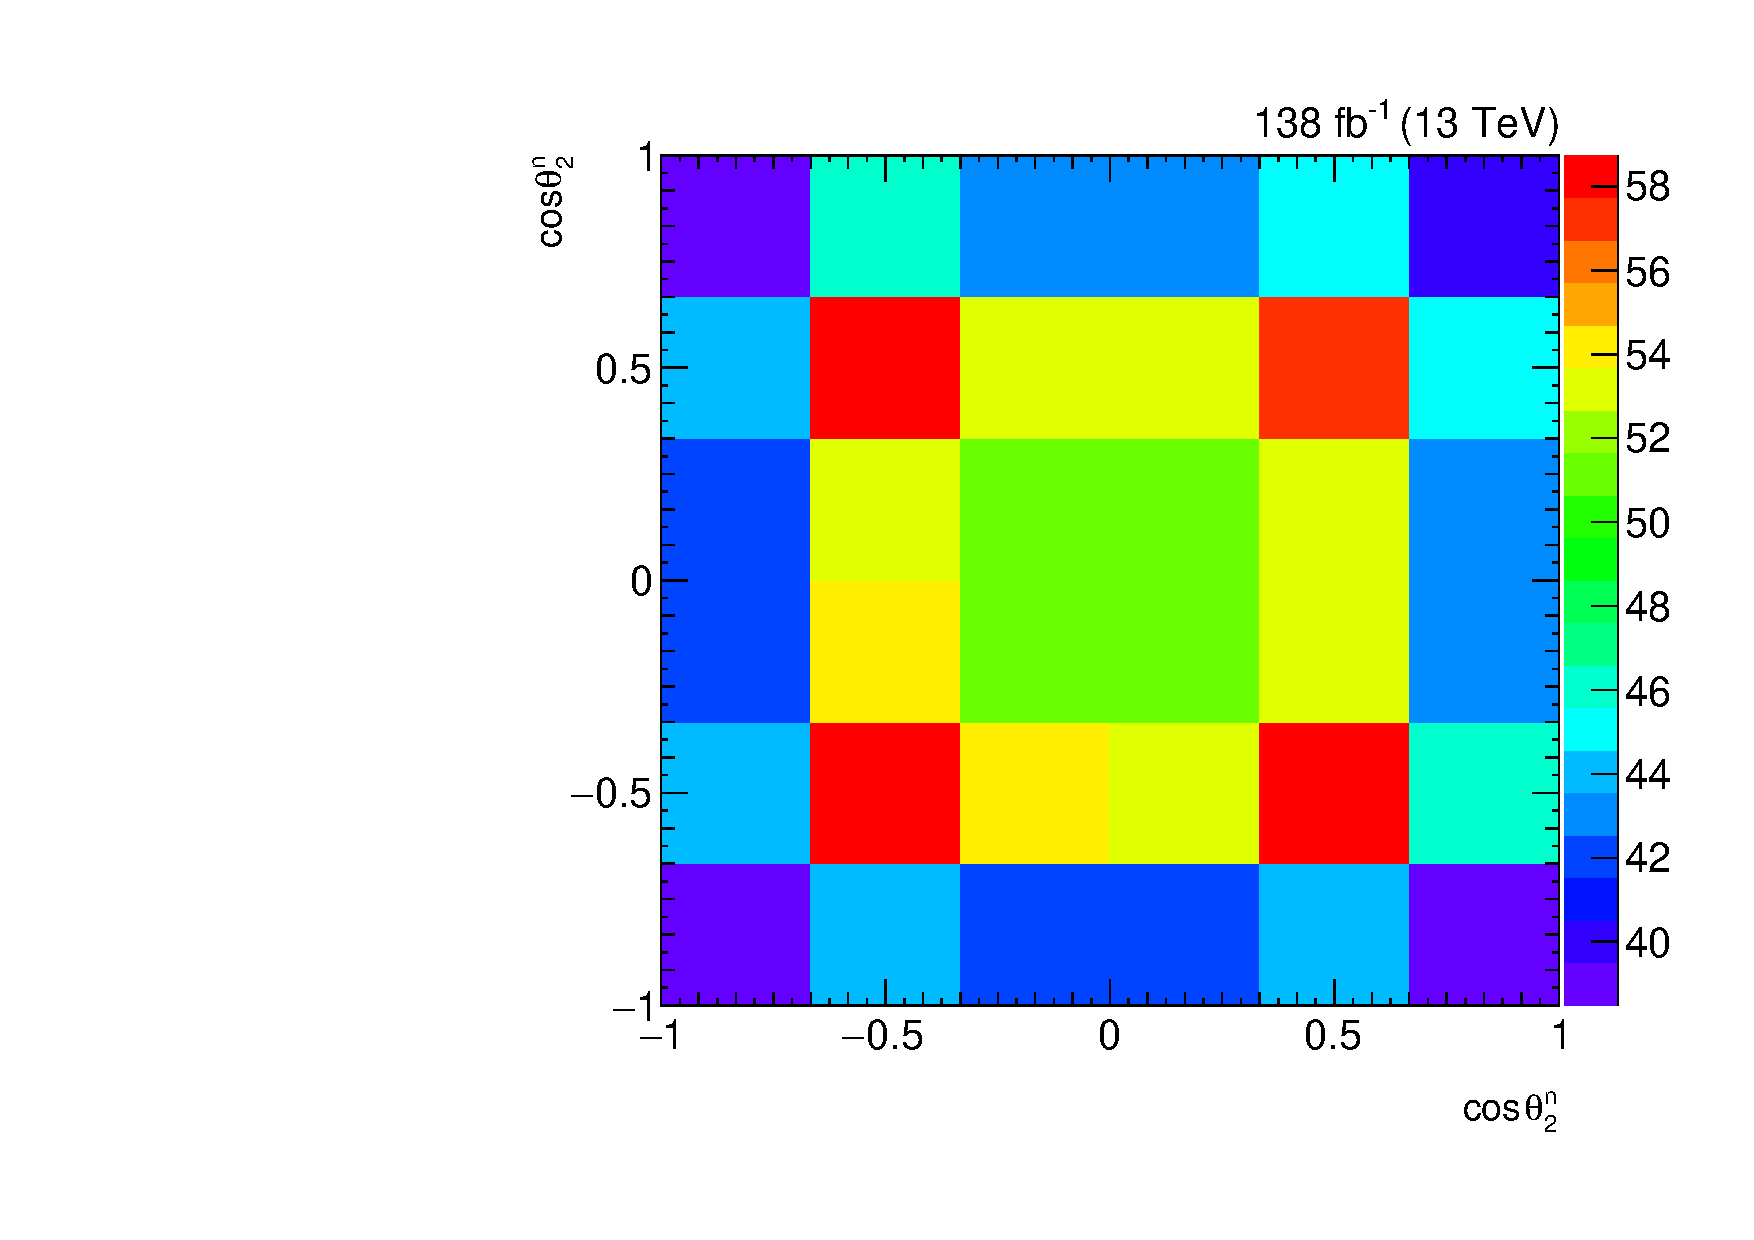
\includegraphics[width=0.32\textwidth]{fig_fullRun2UL/unfolding/combined/TotalSystCovMatrix_rebinnedB_b2n.pdf} \\
 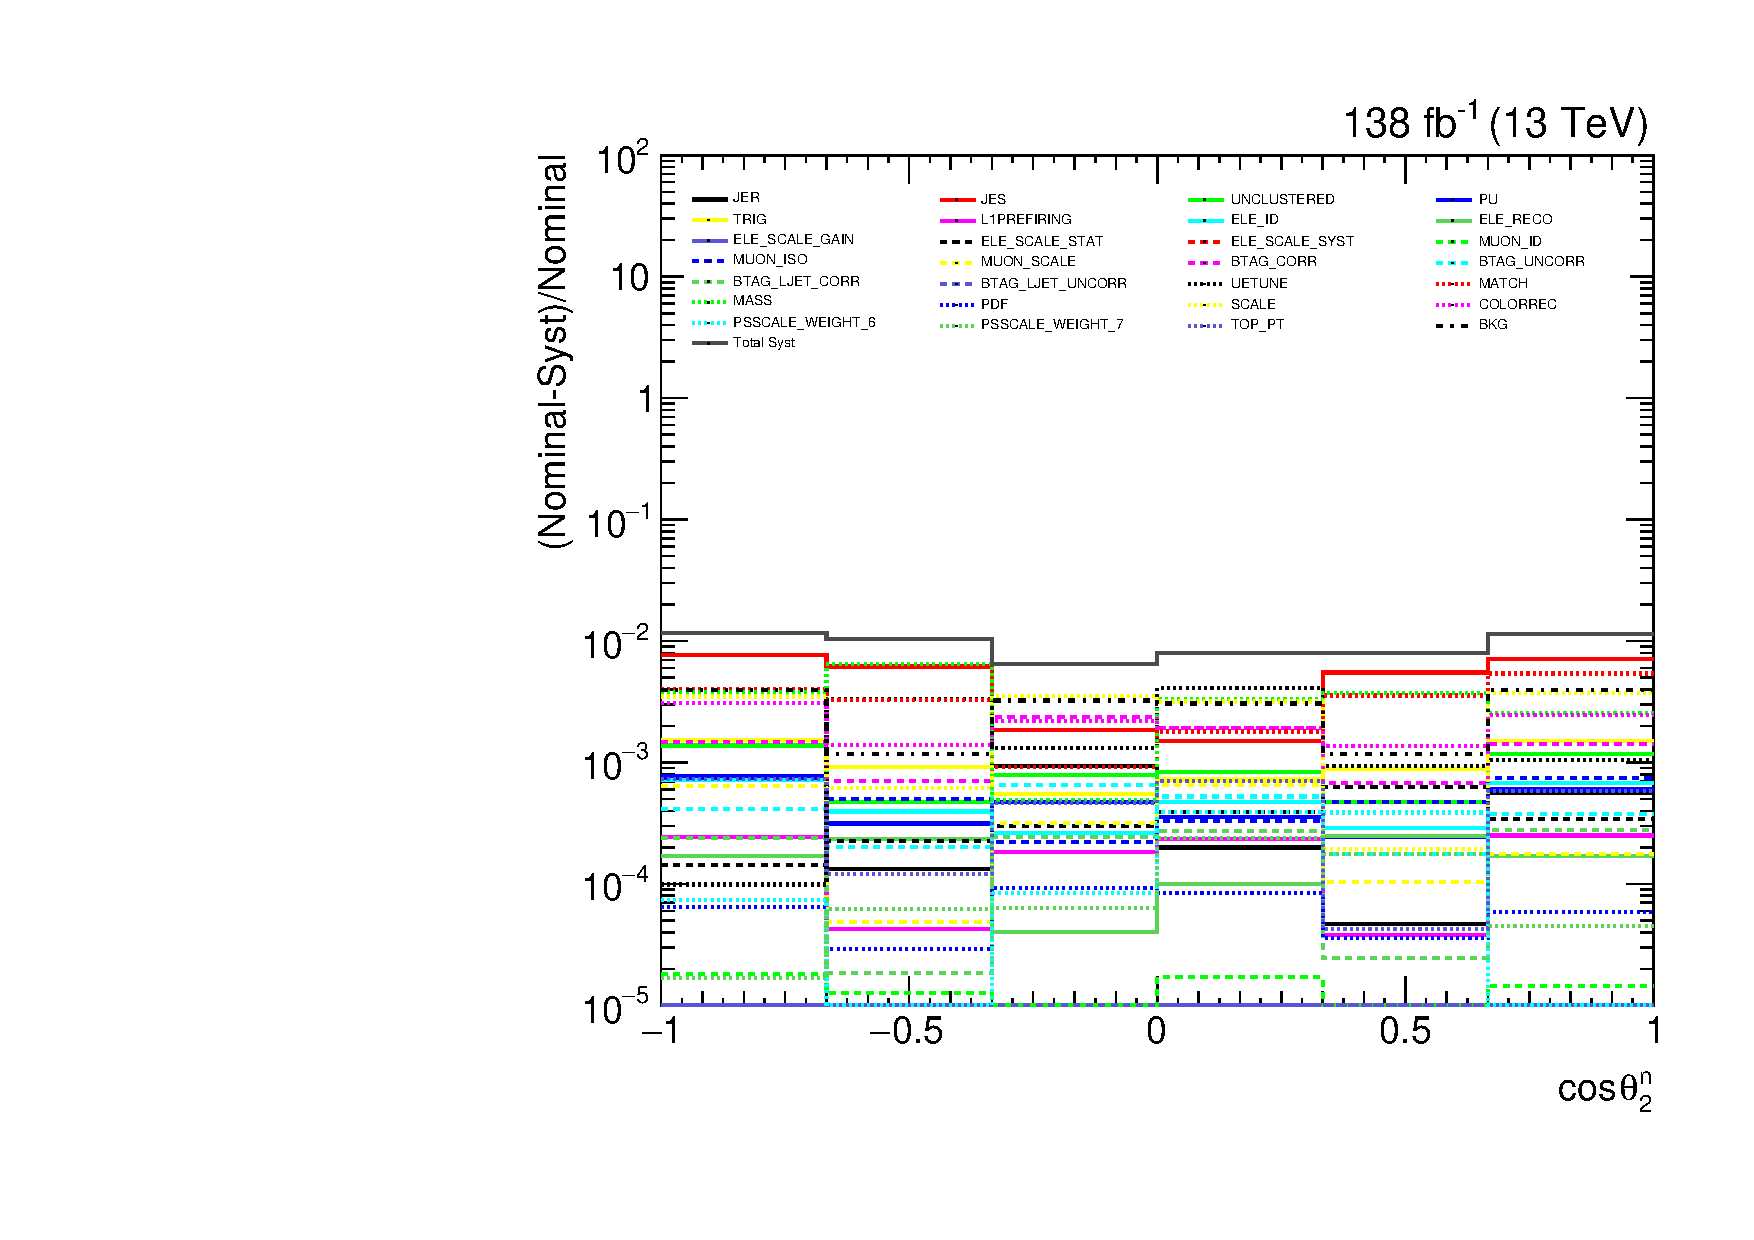
\includegraphics[width=0.32\textwidth]{fig_fullRun2UL/unfolding/combined/deltaSystCombinedlogNorm_rebinnedB_b2n.pdf}
 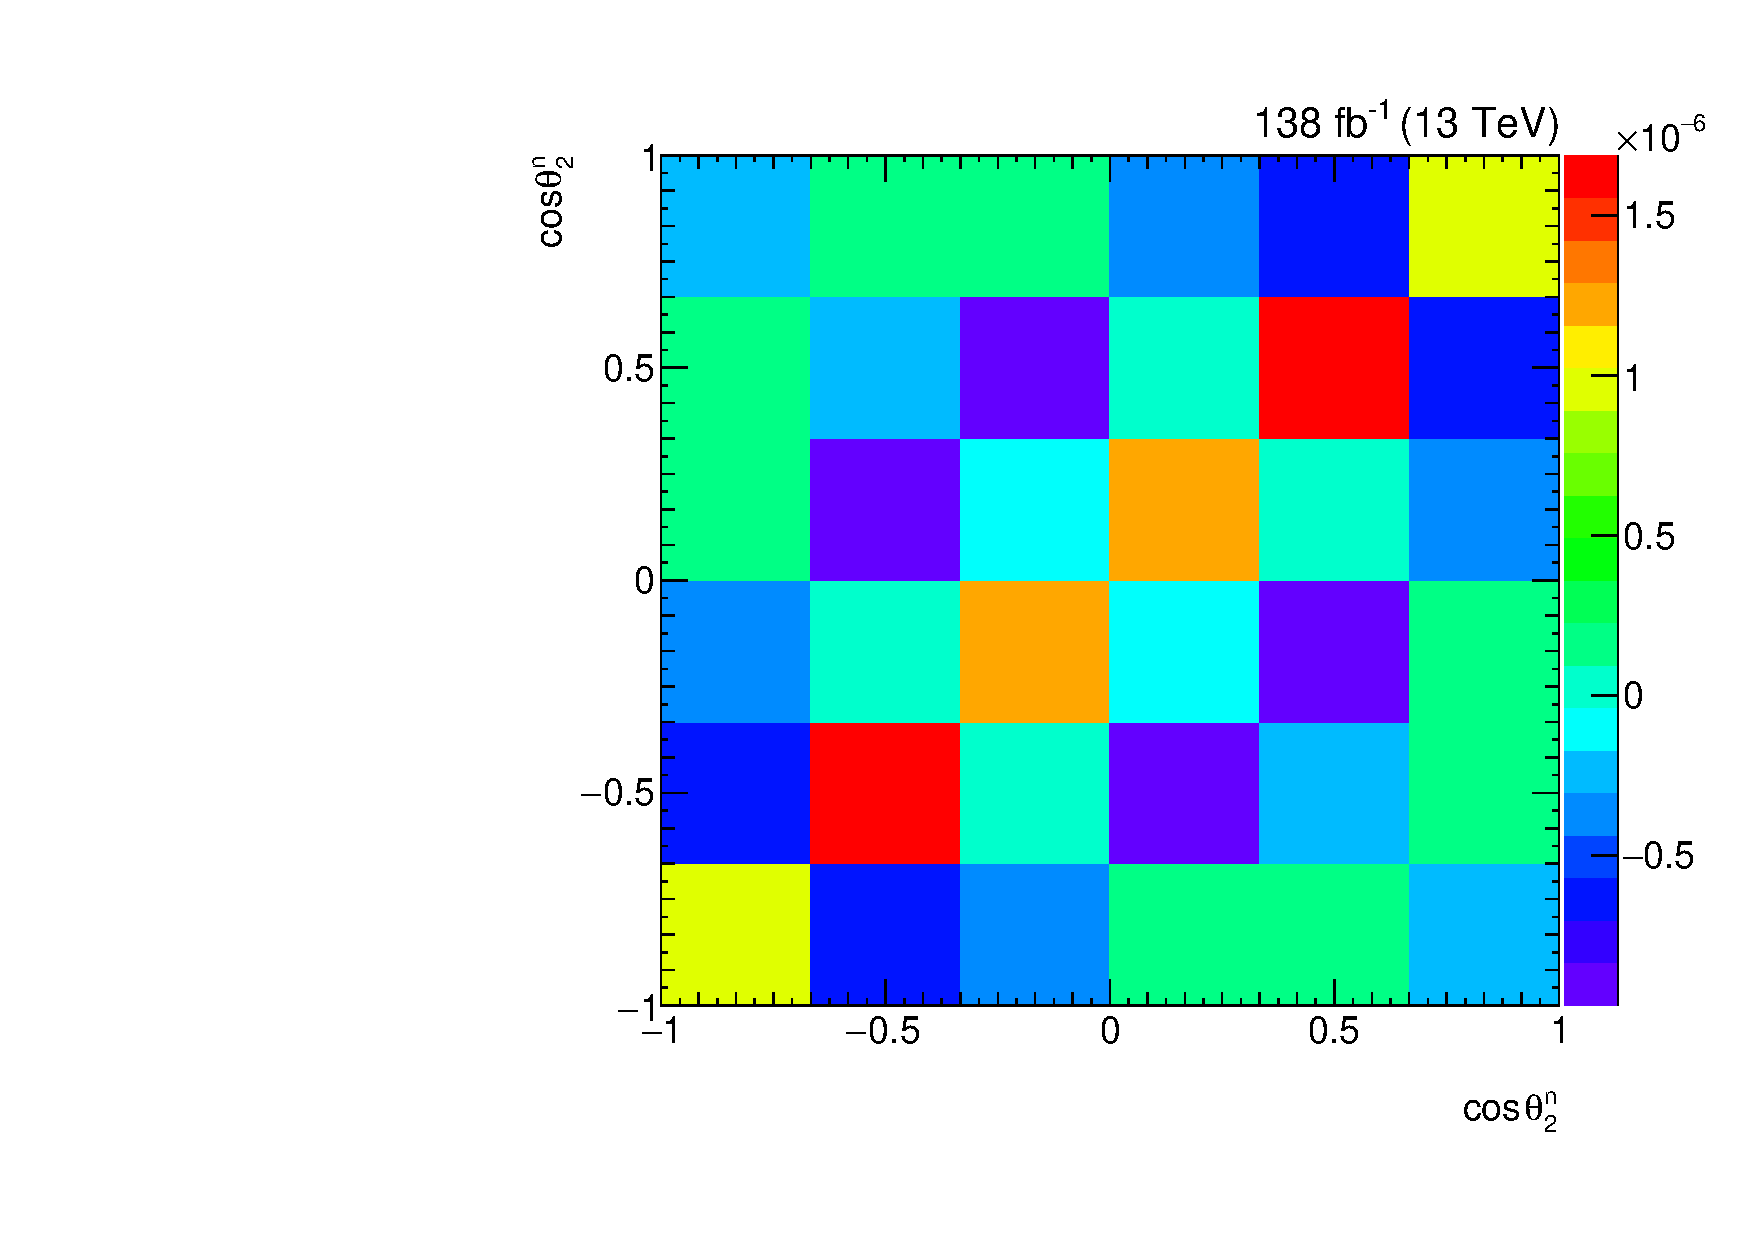
\includegraphics[width=0.32\textwidth]{fig_fullRun2UL/unfolding/combined/StatCovMatrixNorm_rebinnedB_b2n.pdf}
 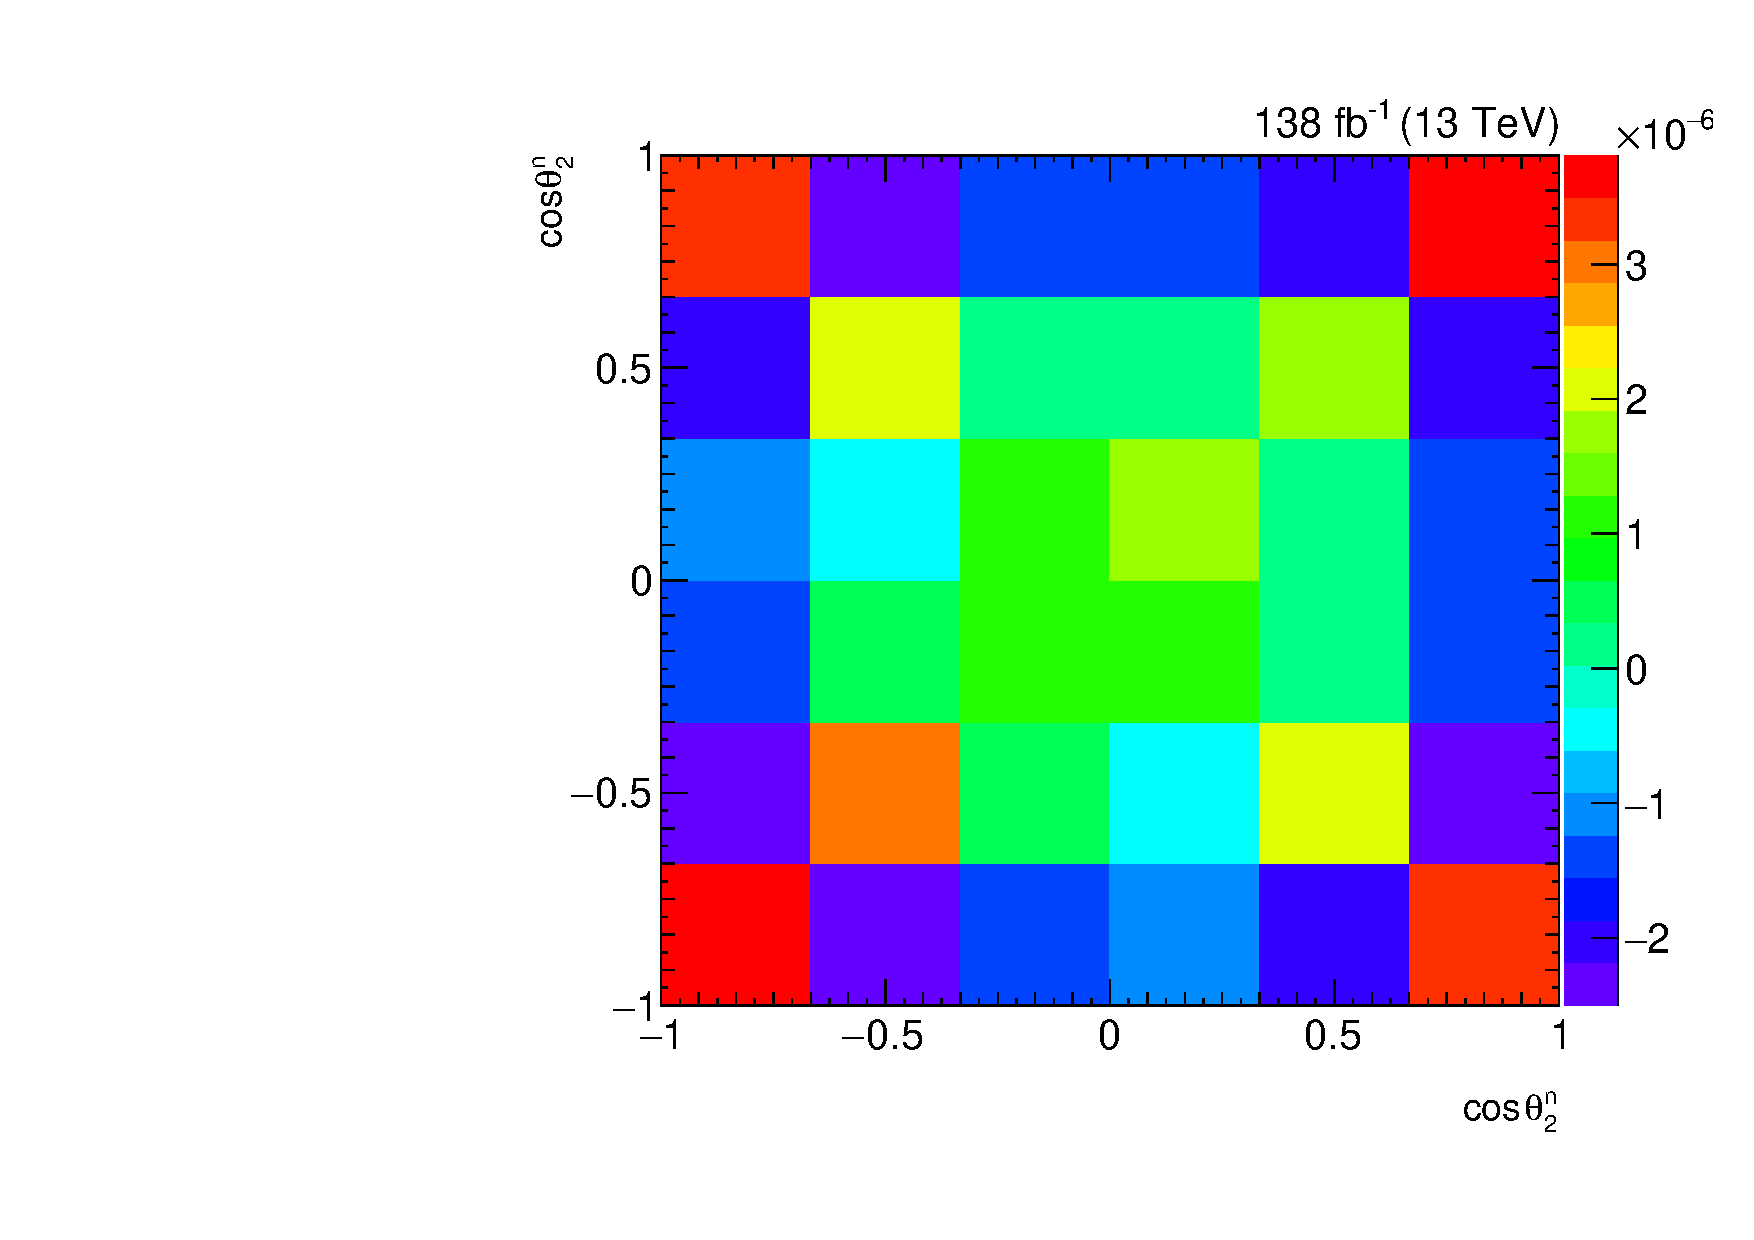
\includegraphics[width=0.32\textwidth]{fig_fullRun2UL/unfolding/combined/TotalSystCovMatrixNorm_rebinnedB_b2n.pdf} \\
\caption{Unfolded-cross section breakdown of uncertainties (Top Left), unfolded cross-section statistical covariance matrix (Top Middle), unfolded cross-section total systematic covariance matrix (Top Right), normalized unfolded-cross section breakdown of uncertainties (Bottom Left), normalized unfolded cross-section statistical covariance matrix (Bottom Middle), normalized unfolded cross-section total systematic covariance matrix (Bottom Right) for polarization observable $\cos\theta_{2}^{n}$.}
\label{fig:b2n_uncertainties}
\end{center}
\end{figure}
\clearpage
\begin{figure}[htb]
\begin{center}
 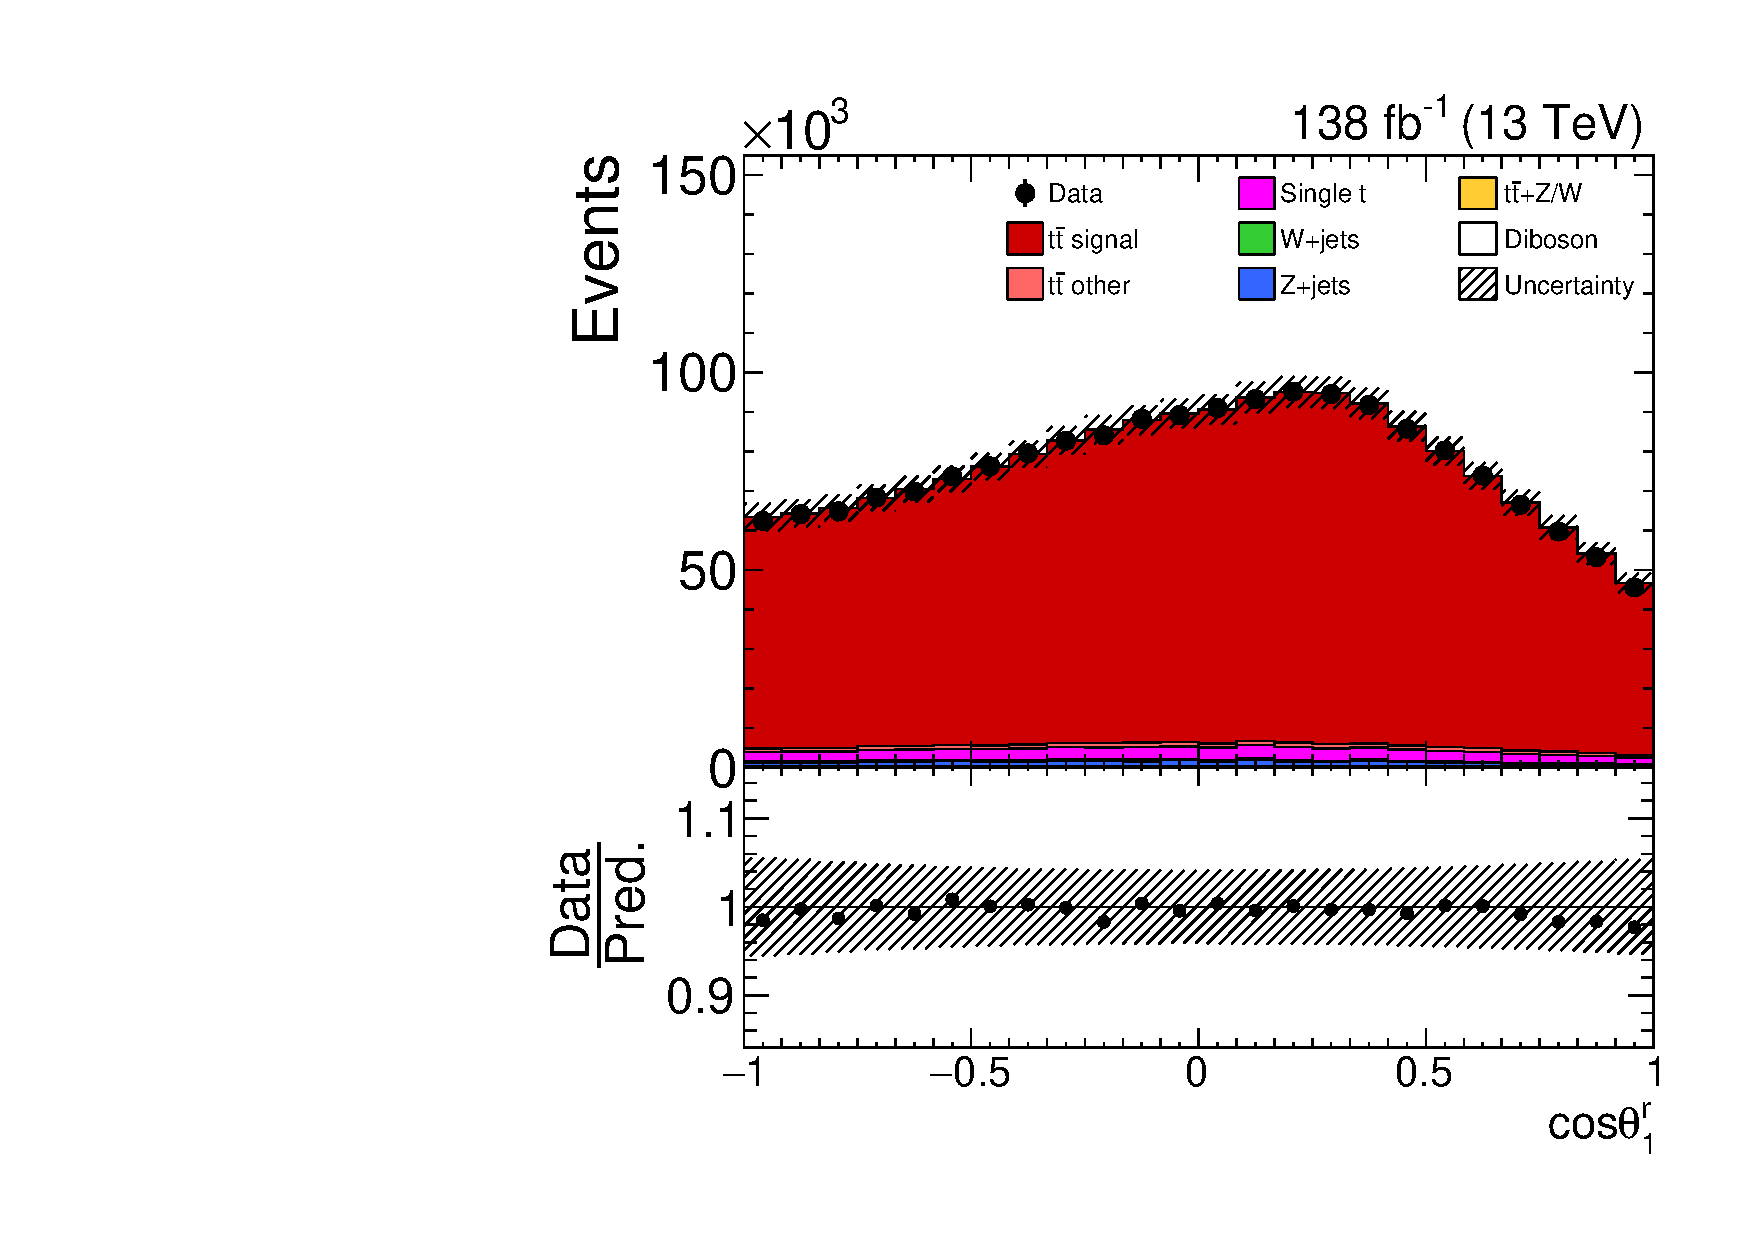
\includegraphics[width=0.32\textwidth]{fig_fullRun2UL/controlplots/combined/Hyp_AntiLeptonBr.pdf}
 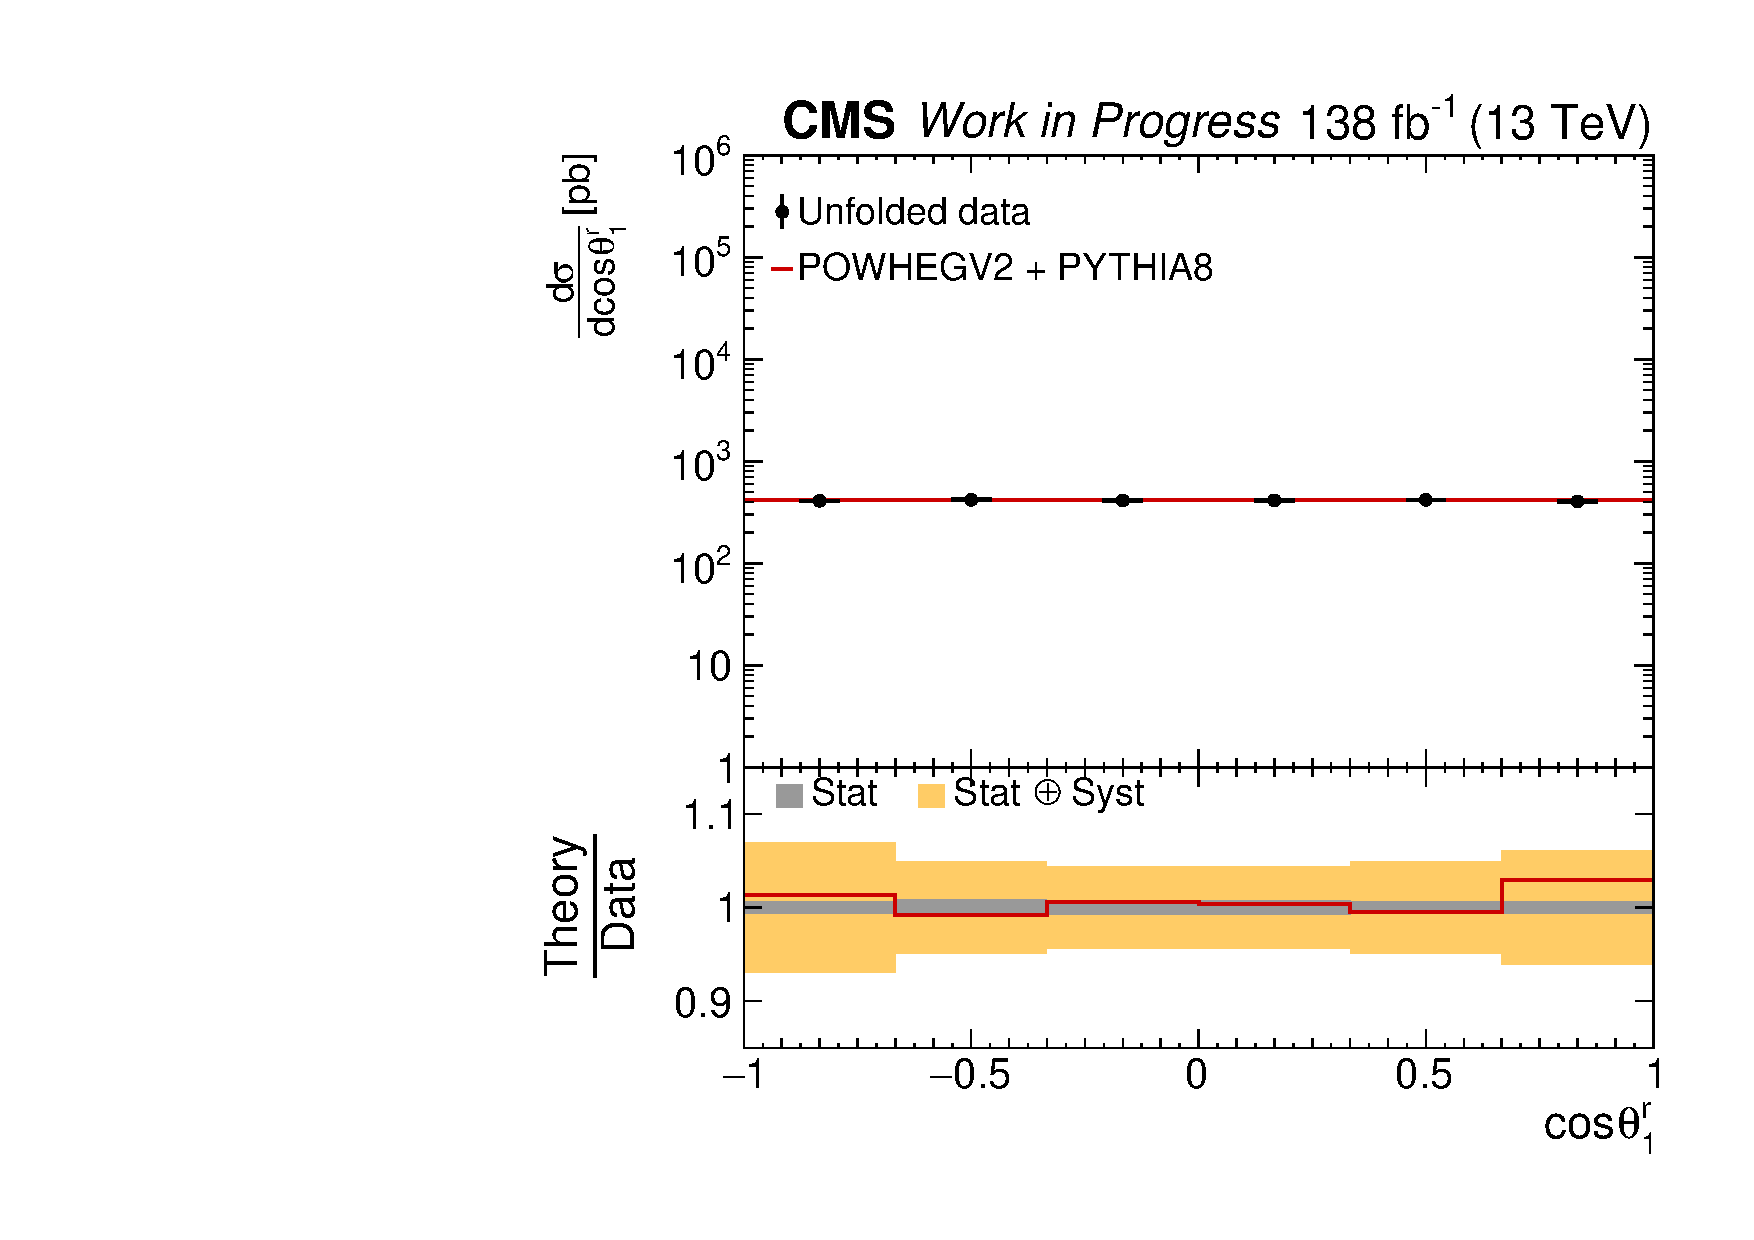
\includegraphics[width=0.32\textwidth]{fig_fullRun2UL/unfolding/combined/UnfoldedResults_b1r.pdf}
 \includegraphics[width=0.32\textwidth]{fig_fullRun2UL/unfolding/combined/UnfoldedResultsNorm_b1r.pdf} \\
 \includegraphics[width=0.32\textwidth]{fig_fullRun2UL/unfolding/combined/ResponseMatrix_b1r.pdf}
 \includegraphics[width=0.32\textwidth]{fig_fullRun2UL/unfolding/combined/TotEff_b1r.pdf}
 \includegraphics[width=0.32\textwidth]{fig_fullRun2UL/unfolding/combined/PurStab_b1r.pdf} \\
\caption{Reconstructed detector-level distribution (Top Left), absolute cross-section unfolded to parton-level (Top Middle), normalized cross-section unfolded to parton-level (Top Right), detector response-matrix (Bottom Left), efficiency$\times$acceptance (Bottom Middle), Purity and Stability (Bottom Right) for polarization observable $\cos\theta_{1}^{r}$, from which spin-density coefficient $B_{1}^{r}$ (sensitive to spin-density coefficient function $b_r^{+}$) is extracted.}
\label{fig:b1r}
\end{center}
\end{figure}
\clearpage
\begin{figure}[htb]
\begin{center}
 \includegraphics[width=0.32\textwidth]{fig_fullRun2UL/unfolding/combined/deltaSystCombinedlog_rebinnedB_b1r.pdf}
 \includegraphics[width=0.32\textwidth]{fig_fullRun2UL/unfolding/combined/StatCovMatrix_rebinnedB_b1r.pdf}
 \includegraphics[width=0.32\textwidth]{fig_fullRun2UL/unfolding/combined/TotalSystCovMatrix_rebinnedB_b1r.pdf} \\
 \includegraphics[width=0.32\textwidth]{fig_fullRun2UL/unfolding/combined/deltaSystCombinedlogNorm_rebinnedB_b1r.pdf}
 \includegraphics[width=0.32\textwidth]{fig_fullRun2UL/unfolding/combined/StatCovMatrixNorm_rebinnedB_b1r.pdf}
 \includegraphics[width=0.32\textwidth]{fig_fullRun2UL/unfolding/combined/TotalSystCovMatrixNorm_rebinnedB_b1r.pdf} \\
\caption{Unfolded-cross section breakdown of uncertainties (Top Left), unfolded cross-section statistical covariance matrix (Top Middle), unfolded cross-section total systematic covariance matrix (Top Right), normalized unfolded-cross section breakdown of uncertainties (Bottom Left), normalized unfolded cross-section statistical covariance matrix (Bottom Middle), normalized unfolded cross-section total systematic covariance matrix (Bottom Right) for polarization observable $\cos\theta_{1}^{r}$.}
\label{fig:b1r_uncertainties}
\end{center}
\end{figure}
\clearpage
\begin{figure}[htb]
\begin{center}
 \includegraphics[width=0.32\textwidth]{fig_fullRun2UL/controlplots/combined/Hyp_LeptonBr.pdf}
 \includegraphics[width=0.32\textwidth]{fig_fullRun2UL/unfolding/combined/UnfoldedResults_b2r.pdf}
 \includegraphics[width=0.32\textwidth]{fig_fullRun2UL/unfolding/combined/UnfoldedResultsNorm_b2r.pdf} \\
 \includegraphics[width=0.32\textwidth]{fig_fullRun2UL/unfolding/combined/ResponseMatrix_b2r.pdf}
 \includegraphics[width=0.32\textwidth]{fig_fullRun2UL/unfolding/combined/TotEff_b2r.pdf}
 \includegraphics[width=0.32\textwidth]{fig_fullRun2UL/unfolding/combined/PurStab_b2r.pdf} \\
\caption{Reconstructed detector-level distribution (Top Left), absolute cross-section unfolded to parton-level (Top Middle), normalized cross-section unfolded to parton-level (Top Right), detector response-matrix (Bottom Left), efficiency$\times$acceptance (Bottom Middle), Purity and Stability (Bottom Right) for polarization observable $\cos\theta_{2}^{r}$, from which spin-density coefficient $B_{2}^{r}$ (sensitive to spin-density coefficient function $b_r^{-}$) is extracted.}
\label{fig:b2r}
\end{center}
\end{figure}
\clearpage
\begin{figure}[htb]
\begin{center}
 \includegraphics[width=0.32\textwidth]{fig_fullRun2UL/unfolding/combined/deltaSystCombinedlog_rebinnedB_b2r.pdf}
 \includegraphics[width=0.32\textwidth]{fig_fullRun2UL/unfolding/combined/StatCovMatrix_rebinnedB_b2r.pdf}
 \includegraphics[width=0.32\textwidth]{fig_fullRun2UL/unfolding/combined/TotalSystCovMatrix_rebinnedB_b2r.pdf} \\
 \includegraphics[width=0.32\textwidth]{fig_fullRun2UL/unfolding/combined/deltaSystCombinedlogNorm_rebinnedB_b2r.pdf}
 \includegraphics[width=0.32\textwidth]{fig_fullRun2UL/unfolding/combined/StatCovMatrixNorm_rebinnedB_b2r.pdf}
 \includegraphics[width=0.32\textwidth]{fig_fullRun2UL/unfolding/combined/TotalSystCovMatrixNorm_rebinnedB_b2r.pdf} \\
\caption{Unfolded-cross section breakdown of uncertainties (Top Left), unfolded cross-section statistical covariance matrix (Top Middle), unfolded cross-section total systematic covariance matrix (Top Right), normalized unfolded-cross section breakdown of uncertainties (Bottom Left), normalized unfolded cross-section statistical covariance matrix (Bottom Middle), normalized unfolded cross-section total systematic covariance matrix (Bottom Right) for polarization observable $\cos\theta_{2}^{r}$.}
\label{fig:b2r_uncertainties}
\end{center}
\end{figure}
\clearpage
\begin{figure}[htb]
\begin{center}
 \includegraphics[width=0.32\textwidth]{fig_fullRun2UL/controlplots/combined/Hyp_LLBarCkk.pdf}
 \includegraphics[width=0.32\textwidth]{fig_fullRun2UL/unfolding/combined/UnfoldedResults_c_kk.pdf}
 \includegraphics[width=0.32\textwidth]{fig_fullRun2UL/unfolding/combined/UnfoldedResultsNorm_c_kk.pdf} \\
 \includegraphics[width=0.32\textwidth]{fig_fullRun2UL/unfolding/combined/ResponseMatrix_c_kk.pdf}
 \includegraphics[width=0.32\textwidth]{fig_fullRun2UL/unfolding/combined/TotEff_c_kk.pdf}
 \includegraphics[width=0.32\textwidth]{fig_fullRun2UL/unfolding/combined/PurStab_c_kk.pdf} \\
\caption{Reconstructed detector-level distribution (Top Left), absolute cross-section unfolded to parton-level (Top Middle), normalized cross-section unfolded to parton-level (Top Right), detector response-matrix (Bottom Left), efficiency$\times$acceptance (Bottom Middle), Purity and Stability (Bottom Right) for diagonal spin correlation observable $\cos\theta_{1}^{k}\cos\theta_{2}^{k}$, from which spin-density coefficient $C_{kk}$ (sensitive to spin-density coefficient function $c_{k k}$) is extracted.}
\label{fig:c_kk}
\end{center}
\end{figure}
\clearpage
\begin{figure}[htb]
\begin{center}
 \includegraphics[width=0.32\textwidth]{fig_fullRun2UL/unfolding/combined/deltaSystCombinedlog_rebinnedB_c_kk.pdf}
 \includegraphics[width=0.32\textwidth]{fig_fullRun2UL/unfolding/combined/StatCovMatrix_rebinnedB_c_kk.pdf}
 \includegraphics[width=0.32\textwidth]{fig_fullRun2UL/unfolding/combined/TotalSystCovMatrix_rebinnedB_c_kk.pdf} \\
 \includegraphics[width=0.32\textwidth]{fig_fullRun2UL/unfolding/combined/deltaSystCombinedlogNorm_rebinnedB_c_kk.pdf}
 \includegraphics[width=0.32\textwidth]{fig_fullRun2UL/unfolding/combined/StatCovMatrixNorm_rebinnedB_c_kk.pdf}
 \includegraphics[width=0.32\textwidth]{fig_fullRun2UL/unfolding/combined/TotalSystCovMatrixNorm_rebinnedB_c_kk.pdf} \\
\caption{Unfolded-cross section breakdown of uncertainties (Top Left), unfolded cross-section statistical covariance matrix (Top Middle), unfolded cross-section total systematic covariance matrix (Top Right), normalized unfolded-cross section breakdown of uncertainties (Bottom Left), normalized unfolded cross-section statistical covariance matrix (Bottom Middle), normalized unfolded cross-section total systematic covariance matrix (Bottom Right) for diagonal spin correlation observable $\cos\theta_{1}^{k}\cos\theta_{2}^{k}$.}
\label{fig:c_kk_uncertainties}
\end{center}
\end{figure}
\clearpage
\begin{figure}[htb]
\begin{center}
 \includegraphics[width=0.32\textwidth]{fig_fullRun2UL/controlplots/combined/Hyp_LLBarCrr.pdf}
 \includegraphics[width=0.32\textwidth]{fig_fullRun2UL/unfolding/combined/UnfoldedResults_c_rr.pdf}
 \includegraphics[width=0.32\textwidth]{fig_fullRun2UL/unfolding/combined/UnfoldedResultsNorm_c_rr.pdf} \\
 \includegraphics[width=0.32\textwidth]{fig_fullRun2UL/unfolding/combined/ResponseMatrix_c_rr.pdf}
 \includegraphics[width=0.32\textwidth]{fig_fullRun2UL/unfolding/combined/TotEff_c_rr.pdf}
 \includegraphics[width=0.32\textwidth]{fig_fullRun2UL/unfolding/combined/PurStab_c_rr.pdf} \\
\caption{Reconstructed detector-level distribution (Top Left), absolute cross-section unfolded to parton-level (Top Middle), normalized cross-section unfolded to parton-level (Top Right), detector response-matrix (Bottom Left), efficiency$\times$acceptance (Bottom Middle), Purity and Stability (Bottom Right) for diagonal spin correlation observable $\cos\theta_{1}^{r}\cos\theta_{2}^{r}$, from which spin-density coefficient $C_{rr}$ (sensitive to spin-density coefficient function $c_{r r}$) is extracted.}
\label{fig:c_rr}
\end{center}
\end{figure}
\clearpage
\begin{figure}[htb]
\begin{center}
 \includegraphics[width=0.32\textwidth]{fig_fullRun2UL/unfolding/combined/deltaSystCombinedlog_rebinnedB_c_rr.pdf}
 \includegraphics[width=0.32\textwidth]{fig_fullRun2UL/unfolding/combined/StatCovMatrix_rebinnedB_c_rr.pdf}
 \includegraphics[width=0.32\textwidth]{fig_fullRun2UL/unfolding/combined/TotalSystCovMatrix_rebinnedB_c_rr.pdf} \\
 \includegraphics[width=0.32\textwidth]{fig_fullRun2UL/unfolding/combined/deltaSystCombinedlogNorm_rebinnedB_c_rr.pdf}
 \includegraphics[width=0.32\textwidth]{fig_fullRun2UL/unfolding/combined/StatCovMatrixNorm_rebinnedB_c_rr.pdf}
 \includegraphics[width=0.32\textwidth]{fig_fullRun2UL/unfolding/combined/TotalSystCovMatrixNorm_rebinnedB_c_rr.pdf} \\
\caption{Unfolded-cross section breakdown of uncertainties (Top Left), unfolded cross-section statistical covariance matrix (Top Middle), unfolded cross-section total systematic covariance matrix (Top Right), normalized unfolded-cross section breakdown of uncertainties (Bottom Left), normalized unfolded cross-section statistical covariance matrix (Bottom Middle), normalized unfolded cross-section total systematic covariance matrix (Bottom Right) for diagonal spin correlation observable $\cos\theta_{1}^{r}\cos\theta_{2}^{r}$.}
\label{fig:c_rr_uncertainties}
\end{center}
\end{figure}
\clearpage
\begin{figure}[htb]
\begin{center}
 \includegraphics[width=0.32\textwidth]{fig_fullRun2UL/controlplots/combined/Hyp_LLBarCnn.pdf}
 \includegraphics[width=0.32\textwidth]{fig_fullRun2UL/unfolding/combined/UnfoldedResults_c_nn.pdf}
 \includegraphics[width=0.32\textwidth]{fig_fullRun2UL/unfolding/combined/UnfoldedResultsNorm_c_nn.pdf} \\
 \includegraphics[width=0.32\textwidth]{fig_fullRun2UL/unfolding/combined/ResponseMatrix_c_nn.pdf}
 \includegraphics[width=0.32\textwidth]{fig_fullRun2UL/unfolding/combined/TotEff_c_nn.pdf}
 \includegraphics[width=0.32\textwidth]{fig_fullRun2UL/unfolding/combined/PurStab_c_nn.pdf} \\
\caption{Reconstructed detector-level distribution (Top Left), absolute cross-section unfolded to parton-level (Top Middle), normalized cross-section unfolded to parton-level (Top Right), detector response-matrix (Bottom Left), efficiency$\times$acceptance (Bottom Middle), Purity and Stability (Bottom Right) for diagonal spin correlation observable $\cos\theta_{1}^{n}\cos\theta_{2}^{n}$, from which spin-density coefficient $C_{nn}$ (sensitive to spin-density coefficient function $c_{n n}$) is extracted.}
\label{fig:c_nn}
\end{center}
\end{figure}
\clearpage
\begin{figure}[htb]
\begin{center}
 \includegraphics[width=0.32\textwidth]{fig_fullRun2UL/unfolding/combined/deltaSystCombinedlog_rebinnedB_c_nn.pdf}
 \includegraphics[width=0.32\textwidth]{fig_fullRun2UL/unfolding/combined/StatCovMatrix_rebinnedB_c_nn.pdf}
 \includegraphics[width=0.32\textwidth]{fig_fullRun2UL/unfolding/combined/TotalSystCovMatrix_rebinnedB_c_nn.pdf} \\
 \includegraphics[width=0.32\textwidth]{fig_fullRun2UL/unfolding/combined/deltaSystCombinedlogNorm_rebinnedB_c_nn.pdf}
 \includegraphics[width=0.32\textwidth]{fig_fullRun2UL/unfolding/combined/StatCovMatrixNorm_rebinnedB_c_nn.pdf}
 \includegraphics[width=0.32\textwidth]{fig_fullRun2UL/unfolding/combined/TotalSystCovMatrixNorm_rebinnedB_c_nn.pdf} \\
\caption{Unfolded-cross section breakdown of uncertainties (Top Left), unfolded cross-section statistical covariance matrix (Top Middle), unfolded cross-section total systematic covariance matrix (Top Right), normalized unfolded-cross section breakdown of uncertainties (Bottom Left), normalized unfolded cross-section statistical covariance matrix (Bottom Middle), normalized unfolded cross-section total systematic covariance matrix (Bottom Right) for diagonal spin correlation observable $\cos\theta_{1}^{n}\cos\theta_{2}^{n}$.}
\label{fig:c_nn_uncertainties}
\end{center}
\end{figure}
\clearpage
\begin{figure}[htb]
\begin{center}
 \includegraphics[width=0.32\textwidth]{fig_fullRun2UL/controlplots/combined/Hyp_LLBarCPrk.pdf}
 \includegraphics[width=0.32\textwidth]{fig_fullRun2UL/unfolding/combined/UnfoldedResults_c_Prk.pdf}
 \includegraphics[width=0.32\textwidth]{fig_fullRun2UL/unfolding/combined/UnfoldedResultsNorm_c_Prk.pdf} \\
 \includegraphics[width=0.32\textwidth]{fig_fullRun2UL/unfolding/combined/ResponseMatrix_c_Prk.pdf}
 \includegraphics[width=0.32\textwidth]{fig_fullRun2UL/unfolding/combined/TotEff_c_Prk.pdf}
 \includegraphics[width=0.32\textwidth]{fig_fullRun2UL/unfolding/combined/PurStab_c_Prk.pdf} \\
\caption{Reconstructed detector-level distribution (Top Left), absolute cross-section unfolded to parton-level (Top Middle), normalized cross-section unfolded to parton-level (Top Right), detector response-matrix (Bottom Left), efficiency$\times$acceptance (Bottom Middle), Purity and Stability (Bottom Right) for off-diagonal spin correlation sum observable $\cos\theta_{1}^{r}\cos\theta_{2}^{k}+\cos\theta_{1}^{k}\cos\theta_{2}^{r}$, from which spin-density coefficient $C_{rk}+C_{kr}$ (sensitive to spin-density coefficient function $c_{r k}$) is extracted.}
\label{fig:c_Prk}
\end{center}
\end{figure}
\clearpage
\begin{figure}[htb]
\begin{center}
 \includegraphics[width=0.32\textwidth]{fig_fullRun2UL/unfolding/combined/deltaSystCombinedlog_rebinnedB_c_Prk.pdf}
 \includegraphics[width=0.32\textwidth]{fig_fullRun2UL/unfolding/combined/StatCovMatrix_rebinnedB_c_Prk.pdf}
 \includegraphics[width=0.32\textwidth]{fig_fullRun2UL/unfolding/combined/TotalSystCovMatrix_rebinnedB_c_Prk.pdf} \\
 \includegraphics[width=0.32\textwidth]{fig_fullRun2UL/unfolding/combined/deltaSystCombinedlogNorm_rebinnedB_c_Prk.pdf}
 \includegraphics[width=0.32\textwidth]{fig_fullRun2UL/unfolding/combined/StatCovMatrixNorm_rebinnedB_c_Prk.pdf}
 \includegraphics[width=0.32\textwidth]{fig_fullRun2UL/unfolding/combined/TotalSystCovMatrixNorm_rebinnedB_c_Prk.pdf} \\
\caption{Unfolded-cross section breakdown of uncertainties (Top Left), unfolded cross-section statistical covariance matrix (Top Middle), unfolded cross-section total systematic covariance matrix (Top Right), normalized unfolded-cross section breakdown of uncertainties (Bottom Left), normalized unfolded cross-section statistical covariance matrix (Bottom Middle), normalized unfolded cross-section total systematic covariance matrix (Bottom Right) for off-diagonal spin correlation sum observable $\cos\theta_{1}^{r}\cos\theta_{2}^{k}+\cos\theta_{1}^{k}\cos\theta_{2}^{r}$.}
\label{fig:c_Prk_uncertainties}
\end{center}
\end{figure}
\clearpage
\begin{figure}[htb]
\begin{center}
 \includegraphics[width=0.32\textwidth]{fig_fullRun2UL/controlplots/combined/Hyp_LLBarCMrk.pdf}
 \includegraphics[width=0.32\textwidth]{fig_fullRun2UL/unfolding/combined/UnfoldedResults_c_Mrk.pdf}
 \includegraphics[width=0.32\textwidth]{fig_fullRun2UL/unfolding/combined/UnfoldedResultsNorm_c_Mrk.pdf} \\
 \includegraphics[width=0.32\textwidth]{fig_fullRun2UL/unfolding/combined/ResponseMatrix_c_Mrk.pdf}
 \includegraphics[width=0.32\textwidth]{fig_fullRun2UL/unfolding/combined/TotEff_c_Mrk.pdf}
 \includegraphics[width=0.32\textwidth]{fig_fullRun2UL/unfolding/combined/PurStab_c_Mrk.pdf} \\
\caption{Reconstructed detector-level distribution (Top Left), absolute cross-section unfolded to parton-level (Top Middle), normalized cross-section unfolded to parton-level (Top Right), detector response-matrix (Bottom Left), efficiency$\times$acceptance (Bottom Middle), Purity and Stability (Bottom Right) for off-diagonal spin correlation difference observable $\cos\theta_{1}^{r}\cos\theta_{2}^{k}-\cos\theta_{1}^{k}\cos\theta_{2}^{r}$, from which spin-density coefficient $C_{rk}-C_{kr}$ (sensitive to spin-density coefficient function $c_n$) is extracted.}
\label{fig:c_Mrk}
\end{center}
\end{figure}
\clearpage
\begin{figure}[htb]
\begin{center}
 \includegraphics[width=0.32\textwidth]{fig_fullRun2UL/unfolding/combined/deltaSystCombinedlog_rebinnedB_c_Mrk.pdf}
 \includegraphics[width=0.32\textwidth]{fig_fullRun2UL/unfolding/combined/StatCovMatrix_rebinnedB_c_Mrk.pdf}
 \includegraphics[width=0.32\textwidth]{fig_fullRun2UL/unfolding/combined/TotalSystCovMatrix_rebinnedB_c_Mrk.pdf} \\
 \includegraphics[width=0.32\textwidth]{fig_fullRun2UL/unfolding/combined/deltaSystCombinedlogNorm_rebinnedB_c_Mrk.pdf}
 \includegraphics[width=0.32\textwidth]{fig_fullRun2UL/unfolding/combined/StatCovMatrixNorm_rebinnedB_c_Mrk.pdf}
 \includegraphics[width=0.32\textwidth]{fig_fullRun2UL/unfolding/combined/TotalSystCovMatrixNorm_rebinnedB_c_Mrk.pdf} \\
\caption{Unfolded-cross section breakdown of uncertainties (Top Left), unfolded cross-section statistical covariance matrix (Top Middle), unfolded cross-section total systematic covariance matrix (Top Right), normalized unfolded-cross section breakdown of uncertainties (Bottom Left), normalized unfolded cross-section statistical covariance matrix (Bottom Middle), normalized unfolded cross-section total systematic covariance matrix (Bottom Right) for off-diagonal spin correlation difference observable $\cos\theta_{1}^{r}\cos\theta_{2}^{k}-\cos\theta_{1}^{k}\cos\theta_{2}^{r}$.}
\label{fig:c_Mrk_uncertainties}
\end{center}
\end{figure}
\clearpage
\begin{figure}[htb]
\begin{center}
 \includegraphics[width=0.32\textwidth]{fig_fullRun2UL/controlplots/combined/Hyp_LLBarCPnr.pdf}
 \includegraphics[width=0.32\textwidth]{fig_fullRun2UL/unfolding/combined/UnfoldedResults_c_Pnr.pdf}
 \includegraphics[width=0.32\textwidth]{fig_fullRun2UL/unfolding/combined/UnfoldedResultsNorm_c_Pnr.pdf} \\
 \includegraphics[width=0.32\textwidth]{fig_fullRun2UL/unfolding/combined/ResponseMatrix_c_Pnr.pdf}
 \includegraphics[width=0.32\textwidth]{fig_fullRun2UL/unfolding/combined/TotEff_c_Pnr.pdf}
 \includegraphics[width=0.32\textwidth]{fig_fullRun2UL/unfolding/combined/PurStab_c_Pnr.pdf} \\
\caption{Reconstructed detector-level distribution (Top Left), absolute cross-section unfolded to parton-level (Top Middle), normalized cross-section unfolded to parton-level (Top Right), detector response-matrix (Bottom Left), efficiency$\times$acceptance (Bottom Middle), Purity and Stability (Bottom Right) for off-diagonal spin correlation sum observable $\cos\theta_{1}^{n}\cos\theta_{2}^{r}+\cos\theta_{1}^{r}\cos\theta_{2}^{n}$, from which spin-density coefficient $C_{nr}+C_{rn}$ (sensitive to spin-density coefficient function $c_{n r}$) is extracted.}
\label{fig:c_Pnr}
\end{center}
\end{figure}
\clearpage
\begin{figure}[htb]
\begin{center}
 \includegraphics[width=0.32\textwidth]{fig_fullRun2UL/unfolding/combined/deltaSystCombinedlog_rebinnedB_c_Pnr.pdf}
 \includegraphics[width=0.32\textwidth]{fig_fullRun2UL/unfolding/combined/StatCovMatrix_rebinnedB_c_Pnr.pdf}
 \includegraphics[width=0.32\textwidth]{fig_fullRun2UL/unfolding/combined/TotalSystCovMatrix_rebinnedB_c_Pnr.pdf} \\
 \includegraphics[width=0.32\textwidth]{fig_fullRun2UL/unfolding/combined/deltaSystCombinedlogNorm_rebinnedB_c_Pnr.pdf}
 \includegraphics[width=0.32\textwidth]{fig_fullRun2UL/unfolding/combined/StatCovMatrixNorm_rebinnedB_c_Pnr.pdf}
 \includegraphics[width=0.32\textwidth]{fig_fullRun2UL/unfolding/combined/TotalSystCovMatrixNorm_rebinnedB_c_Pnr.pdf} \\
\caption{Unfolded-cross section breakdown of uncertainties (Top Left), unfolded cross-section statistical covariance matrix (Top Middle), unfolded cross-section total systematic covariance matrix (Top Right), normalized unfolded-cross section breakdown of uncertainties (Bottom Left), normalized unfolded cross-section statistical covariance matrix (Bottom Middle), normalized unfolded cross-section total systematic covariance matrix (Bottom Right) for off-diagonal spin correlation sum observable $\cos\theta_{1}^{n}\cos\theta_{2}^{r}+\cos\theta_{1}^{r}\cos\theta_{2}^{n}$.}
\label{fig:c_Pnr_uncertainties}
\end{center}
\end{figure}
\clearpage
\begin{figure}[htb]
\begin{center}
 \includegraphics[width=0.32\textwidth]{fig_fullRun2UL/controlplots/combined/Hyp_LLBarCMnr.pdf}
 \includegraphics[width=0.32\textwidth]{fig_fullRun2UL/unfolding/combined/UnfoldedResults_c_Mnr.pdf}
 \includegraphics[width=0.32\textwidth]{fig_fullRun2UL/unfolding/combined/UnfoldedResultsNorm_c_Mnr.pdf} \\
 \includegraphics[width=0.32\textwidth]{fig_fullRun2UL/unfolding/combined/ResponseMatrix_c_Mnr.pdf}
 \includegraphics[width=0.32\textwidth]{fig_fullRun2UL/unfolding/combined/TotEff_c_Mnr.pdf}
 \includegraphics[width=0.32\textwidth]{fig_fullRun2UL/unfolding/combined/PurStab_c_Mnr.pdf} \\
\caption{Reconstructed detector-level distribution (Top Left), absolute cross-section unfolded to parton-level (Top Middle), normalized cross-section unfolded to parton-level (Top Right), detector response-matrix (Bottom Left), efficiency$\times$acceptance (Bottom Middle), Purity and Stability (Bottom Right) for off-diagonal spin correlation difference observable $\cos\theta_{1}^{n}\cos\theta_{2}^{r}-\cos\theta_{1}^{r}\cos\theta_{2}^{n}$, from which spin-density coefficient $C_{nr}-C_{rn}$ (sensitive to spin-density coefficient function $c_k$) is extracted.}
\label{fig:c_Mnr}
\end{center}
\end{figure}
\clearpage
\begin{figure}[htb]
\begin{center}
 \includegraphics[width=0.32\textwidth]{fig_fullRun2UL/unfolding/combined/deltaSystCombinedlog_rebinnedB_c_Mnr.pdf}
 \includegraphics[width=0.32\textwidth]{fig_fullRun2UL/unfolding/combined/StatCovMatrix_rebinnedB_c_Mnr.pdf}
 \includegraphics[width=0.32\textwidth]{fig_fullRun2UL/unfolding/combined/TotalSystCovMatrix_rebinnedB_c_Mnr.pdf} \\
 \includegraphics[width=0.32\textwidth]{fig_fullRun2UL/unfolding/combined/deltaSystCombinedlogNorm_rebinnedB_c_Mnr.pdf}
 \includegraphics[width=0.32\textwidth]{fig_fullRun2UL/unfolding/combined/StatCovMatrixNorm_rebinnedB_c_Mnr.pdf}
 \includegraphics[width=0.32\textwidth]{fig_fullRun2UL/unfolding/combined/TotalSystCovMatrixNorm_rebinnedB_c_Mnr.pdf} \\
\caption{Unfolded-cross section breakdown of uncertainties (Top Left), unfolded cross-section statistical covariance matrix (Top Middle), unfolded cross-section total systematic covariance matrix (Top Right), normalized unfolded-cross section breakdown of uncertainties (Bottom Left), normalized unfolded cross-section statistical covariance matrix (Bottom Middle), normalized unfolded cross-section total systematic covariance matrix (Bottom Right) for off-diagonal spin correlation difference observable $\cos\theta_{1}^{n}\cos\theta_{2}^{r}-\cos\theta_{1}^{r}\cos\theta_{2}^{n}$.}
\label{fig:c_Mnr_uncertainties}
\end{center}
\end{figure}
\clearpage
\begin{figure}[htb]
\begin{center}
 \includegraphics[width=0.32\textwidth]{fig_fullRun2UL/controlplots/combined/Hyp_LLBarCPnk.pdf}
 \includegraphics[width=0.32\textwidth]{fig_fullRun2UL/unfolding/combined/UnfoldedResults_c_Pnk.pdf}
 \includegraphics[width=0.32\textwidth]{fig_fullRun2UL/unfolding/combined/UnfoldedResultsNorm_c_Pnk.pdf} \\
 \includegraphics[width=0.32\textwidth]{fig_fullRun2UL/unfolding/combined/ResponseMatrix_c_Pnk.pdf}
 \includegraphics[width=0.32\textwidth]{fig_fullRun2UL/unfolding/combined/TotEff_c_Pnk.pdf}
 \includegraphics[width=0.32\textwidth]{fig_fullRun2UL/unfolding/combined/PurStab_c_Pnk.pdf} \\
\caption{Reconstructed detector-level distribution (Top Left), absolute cross-section unfolded to parton-level (Top Middle), normalized cross-section unfolded to parton-level (Top Right), detector response-matrix (Bottom Left), efficiency$\times$acceptance (Bottom Middle), Purity and Stability (Bottom Right) for off-diagonal spin correlation sum observable $\cos\theta_{1}^{n}\cos\theta_{2}^{k}+\cos\theta_{1}^{k}\cos\theta_{2}^{n}$, from which spin-density coefficient $C_{nk}+C_{kn}$ (sensitive to spin-density coefficient function $c_{k n}$) is extracted.}
\label{fig:c_Pnk}
\end{center}
\end{figure}
\clearpage
\begin{figure}[htb]
\begin{center}
 \includegraphics[width=0.32\textwidth]{fig_fullRun2UL/unfolding/combined/deltaSystCombinedlog_rebinnedB_c_Pnk.pdf}
 \includegraphics[width=0.32\textwidth]{fig_fullRun2UL/unfolding/combined/StatCovMatrix_rebinnedB_c_Pnk.pdf}
 \includegraphics[width=0.32\textwidth]{fig_fullRun2UL/unfolding/combined/TotalSystCovMatrix_rebinnedB_c_Pnk.pdf} \\
 \includegraphics[width=0.32\textwidth]{fig_fullRun2UL/unfolding/combined/deltaSystCombinedlogNorm_rebinnedB_c_Pnk.pdf}
 \includegraphics[width=0.32\textwidth]{fig_fullRun2UL/unfolding/combined/StatCovMatrixNorm_rebinnedB_c_Pnk.pdf}
 \includegraphics[width=0.32\textwidth]{fig_fullRun2UL/unfolding/combined/TotalSystCovMatrixNorm_rebinnedB_c_Pnk.pdf} \\
\caption{Unfolded-cross section breakdown of uncertainties (Top Left), unfolded cross-section statistical covariance matrix (Top Middle), unfolded cross-section total systematic covariance matrix (Top Right), normalized unfolded-cross section breakdown of uncertainties (Bottom Left), normalized unfolded cross-section statistical covariance matrix (Bottom Middle), normalized unfolded cross-section total systematic covariance matrix (Bottom Right) for off-diagonal spin correlation sum observable $\cos\theta_{1}^{n}\cos\theta_{2}^{k}+\cos\theta_{1}^{k}\cos\theta_{2}^{n}$.}
\label{fig:c_Pnk_uncertainties}
\end{center}
\end{figure}
\clearpage
\begin{figure}[htb]
\begin{center}
 \includegraphics[width=0.32\textwidth]{fig_fullRun2UL/controlplots/combined/Hyp_LLBarCMnk.pdf}
 \includegraphics[width=0.32\textwidth]{fig_fullRun2UL/unfolding/combined/UnfoldedResults_c_Mnk.pdf}
 \includegraphics[width=0.32\textwidth]{fig_fullRun2UL/unfolding/combined/UnfoldedResultsNorm_c_Mnk.pdf} \\
 \includegraphics[width=0.32\textwidth]{fig_fullRun2UL/unfolding/combined/ResponseMatrix_c_Mnk.pdf}
 \includegraphics[width=0.32\textwidth]{fig_fullRun2UL/unfolding/combined/TotEff_c_Mnk.pdf}
 \includegraphics[width=0.32\textwidth]{fig_fullRun2UL/unfolding/combined/PurStab_c_Mnk.pdf} \\
\caption{Reconstructed detector-level distribution (Top Left), absolute cross-section unfolded to parton-level (Top Middle), normalized cross-section unfolded to parton-level (Top Right), detector response-matrix (Bottom Left), efficiency$\times$acceptance (Bottom Middle), Purity and Stability (Bottom Right) for off-diagonal spin correlation difference observable $\cos\theta_{1}^{n}\cos\theta_{2}^{k}-\cos\theta_{1}^{k}\cos\theta_{2}^{n}$, from which spin-density coefficient $C_{nk}-C_{kn}$ (sensitive to spin-density coefficient function $-c_r$) is extracted.}
\label{fig:c_Mnk}
\end{center}
\end{figure}
\clearpage
\begin{figure}[htb]
\begin{center}
 \includegraphics[width=0.32\textwidth]{fig_fullRun2UL/unfolding/combined/deltaSystCombinedlog_rebinnedB_c_Mnk.pdf}
 \includegraphics[width=0.32\textwidth]{fig_fullRun2UL/unfolding/combined/StatCovMatrix_rebinnedB_c_Mnk.pdf}
 \includegraphics[width=0.32\textwidth]{fig_fullRun2UL/unfolding/combined/TotalSystCovMatrix_rebinnedB_c_Mnk.pdf} \\
 \includegraphics[width=0.32\textwidth]{fig_fullRun2UL/unfolding/combined/deltaSystCombinedlogNorm_rebinnedB_c_Mnk.pdf}
 \includegraphics[width=0.32\textwidth]{fig_fullRun2UL/unfolding/combined/StatCovMatrixNorm_rebinnedB_c_Mnk.pdf}
 \includegraphics[width=0.32\textwidth]{fig_fullRun2UL/unfolding/combined/TotalSystCovMatrixNorm_rebinnedB_c_Mnk.pdf} \\
\caption{Unfolded-cross section breakdown of uncertainties (Top Left), unfolded cross-section statistical covariance matrix (Top Middle), unfolded cross-section total systematic covariance matrix (Top Right), normalized unfolded-cross section breakdown of uncertainties (Bottom Left), normalized unfolded cross-section statistical covariance matrix (Bottom Middle), normalized unfolded cross-section total systematic covariance matrix (Bottom Right) for off-diagonal spin correlation difference observable $\cos\theta_{1}^{n}\cos\theta_{2}^{k}-\cos\theta_{1}^{k}\cos\theta_{2}^{n}$.}
\label{fig:c_Mnk_uncertainties}
\end{center}
\end{figure}
\clearpage
\begin{figure}[htb]
\begin{center}
 \includegraphics[width=0.32\textwidth]{fig_fullRun2UL/controlplots/combined/Hyp_LLBarcHel.pdf}
 \includegraphics[width=0.32\textwidth]{fig_fullRun2UL/unfolding/combined/UnfoldedResults_ll_cHel.pdf}
 \includegraphics[width=0.32\textwidth]{fig_fullRun2UL/unfolding/combined/UnfoldedResultsNorm_ll_cHel.pdf} \\
 \includegraphics[width=0.32\textwidth]{fig_fullRun2UL/unfolding/combined/ResponseMatrix_ll_cHel.pdf}
 \includegraphics[width=0.32\textwidth]{fig_fullRun2UL/unfolding/combined/TotEff_ll_cHel.pdf}
 \includegraphics[width=0.32\textwidth]{fig_fullRun2UL/unfolding/combined/PurStab_ll_cHel.pdf} \\
\caption{Reconstructed detector-level distribution (Top Left), absolute cross-section unfolded to parton-level (Top Middle), normalized cross-section unfolded to parton-level (Top Right), detector response-matrix (Bottom Left), efficiency$\times$acceptance (Bottom Middle), Purity and Stability (Bottom Right) for  observable $\cos\varphi$, from which spin-density coefficient $D = -\frac{1}{3}(C_{kk} + C_{rr} + C_{nn})$ (sensitive to spin-density coefficient function $-\frac{1}{3}(c_{kk} + c_{rr} + c_{nn})$) is extracted.}
\label{fig:ll_cHel}
\end{center}
\end{figure}
\clearpage
\begin{figure}[htb]
\begin{center}
 \includegraphics[width=0.32\textwidth]{fig_fullRun2UL/unfolding/combined/deltaSystCombinedlog_rebinnedB_ll_cHel.pdf}
 \includegraphics[width=0.32\textwidth]{fig_fullRun2UL/unfolding/combined/StatCovMatrix_rebinnedB_ll_cHel.pdf}
 \includegraphics[width=0.32\textwidth]{fig_fullRun2UL/unfolding/combined/TotalSystCovMatrix_rebinnedB_ll_cHel.pdf} \\
 \includegraphics[width=0.32\textwidth]{fig_fullRun2UL/unfolding/combined/deltaSystCombinedlogNorm_rebinnedB_ll_cHel.pdf}
 \includegraphics[width=0.32\textwidth]{fig_fullRun2UL/unfolding/combined/StatCovMatrixNorm_rebinnedB_ll_cHel.pdf}
 \includegraphics[width=0.32\textwidth]{fig_fullRun2UL/unfolding/combined/TotalSystCovMatrixNorm_rebinnedB_ll_cHel.pdf} \\
\caption{Unfolded-cross section breakdown of uncertainties (Top Left), unfolded cross-section statistical covariance matrix (Top Middle), unfolded cross-section total systematic covariance matrix (Top Right), normalized unfolded-cross section breakdown of uncertainties (Bottom Left), normalized unfolded cross-section statistical covariance matrix (Bottom Middle), normalized unfolded cross-section total systematic covariance matrix (Bottom Right) for  observable $\cos\varphi$.}
\label{fig:ll_cHel_uncertainties}
\end{center}
\end{figure}
\clearpage
\begin{figure}[htb]
\begin{center}
 \includegraphics[width=0.32\textwidth]{fig_fullRun2UL/controlplots/combined/Hyp_AntiLeptonBk_vs_TTBarMass.pdf}
 \includegraphics[width=0.32\textwidth]{fig_fullRun2UL/unfolding/combined/UnfoldedResults_b1k_mttbar.pdf}
 \includegraphics[width=0.32\textwidth]{fig_fullRun2UL/unfolding/combined/UnfoldedResultsNorm_b1k_mttbar.pdf} \\
 \includegraphics[width=0.32\textwidth]{fig_fullRun2UL/unfolding/combined/ResponseMatrix_b1k_mttbar.pdf}
 \includegraphics[width=0.32\textwidth]{fig_fullRun2UL/unfolding/combined/TotEff_b1k_mttbar.pdf}
 \includegraphics[width=0.32\textwidth]{fig_fullRun2UL/unfolding/combined/PurStab_b1k_mttbar.pdf} \\
\caption{Reconstructed detector-level distribution (Top Left), absolute cross-section unfolded to parton-level (Top Middle), normalized cross-section unfolded to parton-level (Top Right), detector response-matrix (Bottom Left), efficiency$\times$acceptance (Bottom Middle), Purity and Stability (Bottom Right) for polarization observable $\cos\theta_{1}^{k}$ as a function of $m_{t\bar{t}}$, from which differential spin-density coefficients $B_{1}^{k}$ (sensitive to spin-density coefficient functions $b_k^{+}$) are extracted.}
\label{fig:b1k_mttbar}
\end{center}
\end{figure}
\clearpage
\begin{figure}[htb]
\begin{center}
 \includegraphics[width=0.32\textwidth]{fig_fullRun2UL/unfolding/combined/deltaSystCombinedlog_rebinnedB_b1k_mttbar.pdf}
 \includegraphics[width=0.32\textwidth]{fig_fullRun2UL/unfolding/combined/StatCovMatrix_rebinnedB_b1k_mttbar.pdf}
 \includegraphics[width=0.32\textwidth]{fig_fullRun2UL/unfolding/combined/TotalSystCovMatrix_rebinnedB_b1k_mttbar.pdf} \\
 \includegraphics[width=0.32\textwidth]{fig_fullRun2UL/unfolding/combined/deltaSystCombinedlogNorm_rebinnedB_b1k_mttbar.pdf}
 \includegraphics[width=0.32\textwidth]{fig_fullRun2UL/unfolding/combined/StatCovMatrixNorm_rebinnedB_b1k_mttbar.pdf}
 \includegraphics[width=0.32\textwidth]{fig_fullRun2UL/unfolding/combined/TotalSystCovMatrixNorm_rebinnedB_b1k_mttbar.pdf} \\
\caption{Unfolded-cross section breakdown of uncertainties (Top Left), unfolded cross-section statistical covariance matrix (Top Middle), unfolded cross-section total systematic covariance matrix (Top Right), normalized unfolded-cross section breakdown of uncertainties (Bottom Left), normalized unfolded cross-section statistical covariance matrix (Bottom Middle), normalized unfolded cross-section total systematic covariance matrix (Bottom Right) for polarization observable $\cos\theta_{1}^{k}$ as a function of $m_{t\bar{t}}$.}
\label{fig:b1k_mttbar_uncertainties}
\end{center}
\end{figure}
\clearpage
\begin{figure}[htb]
\begin{center}
 \includegraphics[width=0.32\textwidth]{fig_fullRun2UL/controlplots/combined/Hyp_LeptonBk_vs_TTBarMass.pdf}
 \includegraphics[width=0.32\textwidth]{fig_fullRun2UL/unfolding/combined/UnfoldedResults_b2k_mttbar.pdf}
 \includegraphics[width=0.32\textwidth]{fig_fullRun2UL/unfolding/combined/UnfoldedResultsNorm_b2k_mttbar.pdf} \\
 \includegraphics[width=0.32\textwidth]{fig_fullRun2UL/unfolding/combined/ResponseMatrix_b2k_mttbar.pdf}
 \includegraphics[width=0.32\textwidth]{fig_fullRun2UL/unfolding/combined/TotEff_b2k_mttbar.pdf}
 \includegraphics[width=0.32\textwidth]{fig_fullRun2UL/unfolding/combined/PurStab_b2k_mttbar.pdf} \\
\caption{Reconstructed detector-level distribution (Top Left), absolute cross-section unfolded to parton-level (Top Middle), normalized cross-section unfolded to parton-level (Top Right), detector response-matrix (Bottom Left), efficiency$\times$acceptance (Bottom Middle), Purity and Stability (Bottom Right) for polarization observable $\cos\theta_{2}^{k}$ as a function of $m_{t\bar{t}}$, from which differential spin-density coefficients $B_{2}^{k}$ (sensitive to spin-density coefficient functions $b_k^{-}$) are extracted.}
\label{fig:b2k_mttbar}
\end{center}
\end{figure}
\clearpage
\begin{figure}[htb]
\begin{center}
 \includegraphics[width=0.32\textwidth]{fig_fullRun2UL/unfolding/combined/deltaSystCombinedlog_rebinnedB_b2k_mttbar.pdf}
 \includegraphics[width=0.32\textwidth]{fig_fullRun2UL/unfolding/combined/StatCovMatrix_rebinnedB_b2k_mttbar.pdf}
 \includegraphics[width=0.32\textwidth]{fig_fullRun2UL/unfolding/combined/TotalSystCovMatrix_rebinnedB_b2k_mttbar.pdf} \\
 \includegraphics[width=0.32\textwidth]{fig_fullRun2UL/unfolding/combined/deltaSystCombinedlogNorm_rebinnedB_b2k_mttbar.pdf}
 \includegraphics[width=0.32\textwidth]{fig_fullRun2UL/unfolding/combined/StatCovMatrixNorm_rebinnedB_b2k_mttbar.pdf}
 \includegraphics[width=0.32\textwidth]{fig_fullRun2UL/unfolding/combined/TotalSystCovMatrixNorm_rebinnedB_b2k_mttbar.pdf} \\
\caption{Unfolded-cross section breakdown of uncertainties (Top Left), unfolded cross-section statistical covariance matrix (Top Middle), unfolded cross-section total systematic covariance matrix (Top Right), normalized unfolded-cross section breakdown of uncertainties (Bottom Left), normalized unfolded cross-section statistical covariance matrix (Bottom Middle), normalized unfolded cross-section total systematic covariance matrix (Bottom Right) for polarization observable $\cos\theta_{2}^{k}$ as a function of $m_{t\bar{t}}$.}
\label{fig:b2k_mttbar_uncertainties}
\end{center}
\end{figure}
\clearpage
\begin{figure}[htb]
\begin{center}
 \includegraphics[width=0.32\textwidth]{fig_fullRun2UL/controlplots/combined/Hyp_AntiLeptonBn_vs_TTBarMass.pdf}
 \includegraphics[width=0.32\textwidth]{fig_fullRun2UL/unfolding/combined/UnfoldedResults_b1n_mttbar.pdf}
 \includegraphics[width=0.32\textwidth]{fig_fullRun2UL/unfolding/combined/UnfoldedResultsNorm_b1n_mttbar.pdf} \\
 \includegraphics[width=0.32\textwidth]{fig_fullRun2UL/unfolding/combined/ResponseMatrix_b1n_mttbar.pdf}
 \includegraphics[width=0.32\textwidth]{fig_fullRun2UL/unfolding/combined/TotEff_b1n_mttbar.pdf}
 \includegraphics[width=0.32\textwidth]{fig_fullRun2UL/unfolding/combined/PurStab_b1n_mttbar.pdf} \\
\caption{Reconstructed detector-level distribution (Top Left), absolute cross-section unfolded to parton-level (Top Middle), normalized cross-section unfolded to parton-level (Top Right), detector response-matrix (Bottom Left), efficiency$\times$acceptance (Bottom Middle), Purity and Stability (Bottom Right) for polarization observable $\cos\theta_{1}^{n}$ as a function of $m_{t\bar{t}}$, from which differential spin-density coefficients $B_{1}^{n}$ (sensitive to spin-density coefficient functions $b_n^{+}$) are extracted.}
\label{fig:b1n_mttbar}
\end{center}
\end{figure}
\clearpage
\begin{figure}[htb]
\begin{center}
 \includegraphics[width=0.32\textwidth]{fig_fullRun2UL/unfolding/combined/deltaSystCombinedlog_rebinnedB_b1n_mttbar.pdf}
 \includegraphics[width=0.32\textwidth]{fig_fullRun2UL/unfolding/combined/StatCovMatrix_rebinnedB_b1n_mttbar.pdf}
 \includegraphics[width=0.32\textwidth]{fig_fullRun2UL/unfolding/combined/TotalSystCovMatrix_rebinnedB_b1n_mttbar.pdf} \\
 \includegraphics[width=0.32\textwidth]{fig_fullRun2UL/unfolding/combined/deltaSystCombinedlogNorm_rebinnedB_b1n_mttbar.pdf}
 \includegraphics[width=0.32\textwidth]{fig_fullRun2UL/unfolding/combined/StatCovMatrixNorm_rebinnedB_b1n_mttbar.pdf}
 \includegraphics[width=0.32\textwidth]{fig_fullRun2UL/unfolding/combined/TotalSystCovMatrixNorm_rebinnedB_b1n_mttbar.pdf} \\
\caption{Unfolded-cross section breakdown of uncertainties (Top Left), unfolded cross-section statistical covariance matrix (Top Middle), unfolded cross-section total systematic covariance matrix (Top Right), normalized unfolded-cross section breakdown of uncertainties (Bottom Left), normalized unfolded cross-section statistical covariance matrix (Bottom Middle), normalized unfolded cross-section total systematic covariance matrix (Bottom Right) for polarization observable $\cos\theta_{1}^{n}$ as a function of $m_{t\bar{t}}$.}
\label{fig:b1n_mttbar_uncertainties}
\end{center}
\end{figure}
\clearpage
\begin{figure}[htb]
\begin{center}
 \includegraphics[width=0.32\textwidth]{fig_fullRun2UL/controlplots/combined/Hyp_LeptonBn_vs_TTBarMass.pdf}
 \includegraphics[width=0.32\textwidth]{fig_fullRun2UL/unfolding/combined/UnfoldedResults_b2n_mttbar.pdf}
 \includegraphics[width=0.32\textwidth]{fig_fullRun2UL/unfolding/combined/UnfoldedResultsNorm_b2n_mttbar.pdf} \\
 \includegraphics[width=0.32\textwidth]{fig_fullRun2UL/unfolding/combined/ResponseMatrix_b2n_mttbar.pdf}
 \includegraphics[width=0.32\textwidth]{fig_fullRun2UL/unfolding/combined/TotEff_b2n_mttbar.pdf}
 \includegraphics[width=0.32\textwidth]{fig_fullRun2UL/unfolding/combined/PurStab_b2n_mttbar.pdf} \\
\caption{Reconstructed detector-level distribution (Top Left), absolute cross-section unfolded to parton-level (Top Middle), normalized cross-section unfolded to parton-level (Top Right), detector response-matrix (Bottom Left), efficiency$\times$acceptance (Bottom Middle), Purity and Stability (Bottom Right) for polarization observable $\cos\theta_{2}^{n}$ as a function of $m_{t\bar{t}}$, from which differential spin-density coefficients $B_{2}^{n}$ (sensitive to spin-density coefficient functions $b_n^{-}$) are extracted.}
\label{fig:b2n_mttbar}
\end{center}
\end{figure}
\clearpage
\begin{figure}[htb]
\begin{center}
 \includegraphics[width=0.32\textwidth]{fig_fullRun2UL/unfolding/combined/deltaSystCombinedlog_rebinnedB_b2n_mttbar.pdf}
 \includegraphics[width=0.32\textwidth]{fig_fullRun2UL/unfolding/combined/StatCovMatrix_rebinnedB_b2n_mttbar.pdf}
 \includegraphics[width=0.32\textwidth]{fig_fullRun2UL/unfolding/combined/TotalSystCovMatrix_rebinnedB_b2n_mttbar.pdf} \\
 \includegraphics[width=0.32\textwidth]{fig_fullRun2UL/unfolding/combined/deltaSystCombinedlogNorm_rebinnedB_b2n_mttbar.pdf}
 \includegraphics[width=0.32\textwidth]{fig_fullRun2UL/unfolding/combined/StatCovMatrixNorm_rebinnedB_b2n_mttbar.pdf}
 \includegraphics[width=0.32\textwidth]{fig_fullRun2UL/unfolding/combined/TotalSystCovMatrixNorm_rebinnedB_b2n_mttbar.pdf} \\
\caption{Unfolded-cross section breakdown of uncertainties (Top Left), unfolded cross-section statistical covariance matrix (Top Middle), unfolded cross-section total systematic covariance matrix (Top Right), normalized unfolded-cross section breakdown of uncertainties (Bottom Left), normalized unfolded cross-section statistical covariance matrix (Bottom Middle), normalized unfolded cross-section total systematic covariance matrix (Bottom Right) for polarization observable $\cos\theta_{2}^{n}$ as a function of $m_{t\bar{t}}$.}
\label{fig:b2n_mttbar_uncertainties}
\end{center}
\end{figure}
\clearpage
\begin{figure}[htb]
\begin{center}
 \includegraphics[width=0.32\textwidth]{fig_fullRun2UL/controlplots/combined/Hyp_AntiLeptonBr_vs_TTBarMass.pdf}
 \includegraphics[width=0.32\textwidth]{fig_fullRun2UL/unfolding/combined/UnfoldedResults_b1r_mttbar.pdf}
 \includegraphics[width=0.32\textwidth]{fig_fullRun2UL/unfolding/combined/UnfoldedResultsNorm_b1r_mttbar.pdf} \\
 \includegraphics[width=0.32\textwidth]{fig_fullRun2UL/unfolding/combined/ResponseMatrix_b1r_mttbar.pdf}
 \includegraphics[width=0.32\textwidth]{fig_fullRun2UL/unfolding/combined/TotEff_b1r_mttbar.pdf}
 \includegraphics[width=0.32\textwidth]{fig_fullRun2UL/unfolding/combined/PurStab_b1r_mttbar.pdf} \\
\caption{Reconstructed detector-level distribution (Top Left), absolute cross-section unfolded to parton-level (Top Middle), normalized cross-section unfolded to parton-level (Top Right), detector response-matrix (Bottom Left), efficiency$\times$acceptance (Bottom Middle), Purity and Stability (Bottom Right) for polarization observable $\cos\theta_{1}^{r}$ as a function of $m_{t\bar{t}}$, from which differential spin-density coefficients $B_{1}^{r}$ (sensitive to spin-density coefficient functions $b_r^{+}$) are extracted.}
\label{fig:b1r_mttbar}
\end{center}
\end{figure}
\clearpage
\begin{figure}[htb]
\begin{center}
 \includegraphics[width=0.32\textwidth]{fig_fullRun2UL/unfolding/combined/deltaSystCombinedlog_rebinnedB_b1r_mttbar.pdf}
 \includegraphics[width=0.32\textwidth]{fig_fullRun2UL/unfolding/combined/StatCovMatrix_rebinnedB_b1r_mttbar.pdf}
 \includegraphics[width=0.32\textwidth]{fig_fullRun2UL/unfolding/combined/TotalSystCovMatrix_rebinnedB_b1r_mttbar.pdf} \\
 \includegraphics[width=0.32\textwidth]{fig_fullRun2UL/unfolding/combined/deltaSystCombinedlogNorm_rebinnedB_b1r_mttbar.pdf}
 \includegraphics[width=0.32\textwidth]{fig_fullRun2UL/unfolding/combined/StatCovMatrixNorm_rebinnedB_b1r_mttbar.pdf}
 \includegraphics[width=0.32\textwidth]{fig_fullRun2UL/unfolding/combined/TotalSystCovMatrixNorm_rebinnedB_b1r_mttbar.pdf} \\
\caption{Unfolded-cross section breakdown of uncertainties (Top Left), unfolded cross-section statistical covariance matrix (Top Middle), unfolded cross-section total systematic covariance matrix (Top Right), normalized unfolded-cross section breakdown of uncertainties (Bottom Left), normalized unfolded cross-section statistical covariance matrix (Bottom Middle), normalized unfolded cross-section total systematic covariance matrix (Bottom Right) for polarization observable $\cos\theta_{1}^{r}$ as a function of $m_{t\bar{t}}$.}
\label{fig:b1r_mttbar_uncertainties}
\end{center}
\end{figure}
\clearpage
\begin{figure}[htb]
\begin{center}
 \includegraphics[width=0.32\textwidth]{fig_fullRun2UL/controlplots/combined/Hyp_LeptonBr_vs_TTBarMass.pdf}
 \includegraphics[width=0.32\textwidth]{fig_fullRun2UL/unfolding/combined/UnfoldedResults_b2r_mttbar.pdf}
 \includegraphics[width=0.32\textwidth]{fig_fullRun2UL/unfolding/combined/UnfoldedResultsNorm_b2r_mttbar.pdf} \\
 \includegraphics[width=0.32\textwidth]{fig_fullRun2UL/unfolding/combined/ResponseMatrix_b2r_mttbar.pdf}
 \includegraphics[width=0.32\textwidth]{fig_fullRun2UL/unfolding/combined/TotEff_b2r_mttbar.pdf}
 \includegraphics[width=0.32\textwidth]{fig_fullRun2UL/unfolding/combined/PurStab_b2r_mttbar.pdf} \\
\caption{Reconstructed detector-level distribution (Top Left), absolute cross-section unfolded to parton-level (Top Middle), normalized cross-section unfolded to parton-level (Top Right), detector response-matrix (Bottom Left), efficiency$\times$acceptance (Bottom Middle), Purity and Stability (Bottom Right) for polarization observable $\cos\theta_{2}^{r}$ as a function of $m_{t\bar{t}}$, from which differential spin-density coefficients $B_{2}^{r}$ (sensitive to spin-density coefficient functions $b_r^{-}$) are extracted.}
\label{fig:b2r_mttbar}
\end{center}
\end{figure}
\clearpage
\begin{figure}[htb]
\begin{center}
 \includegraphics[width=0.32\textwidth]{fig_fullRun2UL/unfolding/combined/deltaSystCombinedlog_rebinnedB_b2r_mttbar.pdf}
 \includegraphics[width=0.32\textwidth]{fig_fullRun2UL/unfolding/combined/StatCovMatrix_rebinnedB_b2r_mttbar.pdf}
 \includegraphics[width=0.32\textwidth]{fig_fullRun2UL/unfolding/combined/TotalSystCovMatrix_rebinnedB_b2r_mttbar.pdf} \\
 \includegraphics[width=0.32\textwidth]{fig_fullRun2UL/unfolding/combined/deltaSystCombinedlogNorm_rebinnedB_b2r_mttbar.pdf}
 \includegraphics[width=0.32\textwidth]{fig_fullRun2UL/unfolding/combined/StatCovMatrixNorm_rebinnedB_b2r_mttbar.pdf}
 \includegraphics[width=0.32\textwidth]{fig_fullRun2UL/unfolding/combined/TotalSystCovMatrixNorm_rebinnedB_b2r_mttbar.pdf} \\
\caption{Unfolded-cross section breakdown of uncertainties (Top Left), unfolded cross-section statistical covariance matrix (Top Middle), unfolded cross-section total systematic covariance matrix (Top Right), normalized unfolded-cross section breakdown of uncertainties (Bottom Left), normalized unfolded cross-section statistical covariance matrix (Bottom Middle), normalized unfolded cross-section total systematic covariance matrix (Bottom Right) for polarization observable $\cos\theta_{2}^{r}$ as a function of $m_{t\bar{t}}$.}
\label{fig:b2r_mttbar_uncertainties}
\end{center}
\end{figure}
\clearpage
\begin{figure}[htb]
\begin{center}
 \includegraphics[width=0.32\textwidth]{fig_fullRun2UL/controlplots/combined/Hyp_LLBarCkk_vs_TTBarMass.pdf}
 \includegraphics[width=0.32\textwidth]{fig_fullRun2UL/unfolding/combined/UnfoldedResults_c_kk_mttbar.pdf}
 \includegraphics[width=0.32\textwidth]{fig_fullRun2UL/unfolding/combined/UnfoldedResultsNorm_c_kk_mttbar.pdf} \\
 \includegraphics[width=0.32\textwidth]{fig_fullRun2UL/unfolding/combined/ResponseMatrix_c_kk_mttbar.pdf}
 \includegraphics[width=0.32\textwidth]{fig_fullRun2UL/unfolding/combined/TotEff_c_kk_mttbar.pdf}
 \includegraphics[width=0.32\textwidth]{fig_fullRun2UL/unfolding/combined/PurStab_c_kk_mttbar.pdf} \\
\caption{Reconstructed detector-level distribution (Top Left), absolute cross-section unfolded to parton-level (Top Middle), normalized cross-section unfolded to parton-level (Top Right), detector response-matrix (Bottom Left), efficiency$\times$acceptance (Bottom Middle), Purity and Stability (Bottom Right) for diagonal spin correlation observable $\cos\theta_{1}^{k}\cos\theta_{2}^{k}$ as a function of $m_{t\bar{t}}$, from which differential spin-density coefficients $C_{kk}$ (sensitive to spin-density coefficient functions $c_{k k}$) are extracted.}
\label{fig:c_kk_mttbar}
\end{center}
\end{figure}
\clearpage
\begin{figure}[htb]
\begin{center}
 \includegraphics[width=0.32\textwidth]{fig_fullRun2UL/unfolding/combined/deltaSystCombinedlog_rebinnedB_c_kk_mttbar.pdf}
 \includegraphics[width=0.32\textwidth]{fig_fullRun2UL/unfolding/combined/StatCovMatrix_rebinnedB_c_kk_mttbar.pdf}
 \includegraphics[width=0.32\textwidth]{fig_fullRun2UL/unfolding/combined/TotalSystCovMatrix_rebinnedB_c_kk_mttbar.pdf} \\
 \includegraphics[width=0.32\textwidth]{fig_fullRun2UL/unfolding/combined/deltaSystCombinedlogNorm_rebinnedB_c_kk_mttbar.pdf}
 \includegraphics[width=0.32\textwidth]{fig_fullRun2UL/unfolding/combined/StatCovMatrixNorm_rebinnedB_c_kk_mttbar.pdf}
 \includegraphics[width=0.32\textwidth]{fig_fullRun2UL/unfolding/combined/TotalSystCovMatrixNorm_rebinnedB_c_kk_mttbar.pdf} \\
\caption{Unfolded-cross section breakdown of uncertainties (Top Left), unfolded cross-section statistical covariance matrix (Top Middle), unfolded cross-section total systematic covariance matrix (Top Right), normalized unfolded-cross section breakdown of uncertainties (Bottom Left), normalized unfolded cross-section statistical covariance matrix (Bottom Middle), normalized unfolded cross-section total systematic covariance matrix (Bottom Right) for diagonal spin correlation observable $\cos\theta_{1}^{k}\cos\theta_{2}^{k}$ as a function of $m_{t\bar{t}}$.}
\label{fig:c_kk_mttbar_uncertainties}
\end{center}
\end{figure}
\clearpage
\begin{figure}[htb]
\begin{center}
 \includegraphics[width=0.32\textwidth]{fig_fullRun2UL/controlplots/combined/Hyp_LLBarCrr_vs_TTBarMass.pdf}
 \includegraphics[width=0.32\textwidth]{fig_fullRun2UL/unfolding/combined/UnfoldedResults_c_rr_mttbar.pdf}
 \includegraphics[width=0.32\textwidth]{fig_fullRun2UL/unfolding/combined/UnfoldedResultsNorm_c_rr_mttbar.pdf} \\
 \includegraphics[width=0.32\textwidth]{fig_fullRun2UL/unfolding/combined/ResponseMatrix_c_rr_mttbar.pdf}
 \includegraphics[width=0.32\textwidth]{fig_fullRun2UL/unfolding/combined/TotEff_c_rr_mttbar.pdf}
 \includegraphics[width=0.32\textwidth]{fig_fullRun2UL/unfolding/combined/PurStab_c_rr_mttbar.pdf} \\
\caption{Reconstructed detector-level distribution (Top Left), absolute cross-section unfolded to parton-level (Top Middle), normalized cross-section unfolded to parton-level (Top Right), detector response-matrix (Bottom Left), efficiency$\times$acceptance (Bottom Middle), Purity and Stability (Bottom Right) for diagonal spin correlation observable $\cos\theta_{1}^{r}\cos\theta_{2}^{r}$ as a function of $m_{t\bar{t}}$, from which differential spin-density coefficients $C_{rr}$ (sensitive to spin-density coefficient functions $c_{r r}$) are extracted.}
\label{fig:c_rr_mttbar}
\end{center}
\end{figure}
\clearpage
\begin{figure}[htb]
\begin{center}
 \includegraphics[width=0.32\textwidth]{fig_fullRun2UL/unfolding/combined/deltaSystCombinedlog_rebinnedB_c_rr_mttbar.pdf}
 \includegraphics[width=0.32\textwidth]{fig_fullRun2UL/unfolding/combined/StatCovMatrix_rebinnedB_c_rr_mttbar.pdf}
 \includegraphics[width=0.32\textwidth]{fig_fullRun2UL/unfolding/combined/TotalSystCovMatrix_rebinnedB_c_rr_mttbar.pdf} \\
 \includegraphics[width=0.32\textwidth]{fig_fullRun2UL/unfolding/combined/deltaSystCombinedlogNorm_rebinnedB_c_rr_mttbar.pdf}
 \includegraphics[width=0.32\textwidth]{fig_fullRun2UL/unfolding/combined/StatCovMatrixNorm_rebinnedB_c_rr_mttbar.pdf}
 \includegraphics[width=0.32\textwidth]{fig_fullRun2UL/unfolding/combined/TotalSystCovMatrixNorm_rebinnedB_c_rr_mttbar.pdf} \\
\caption{Unfolded-cross section breakdown of uncertainties (Top Left), unfolded cross-section statistical covariance matrix (Top Middle), unfolded cross-section total systematic covariance matrix (Top Right), normalized unfolded-cross section breakdown of uncertainties (Bottom Left), normalized unfolded cross-section statistical covariance matrix (Bottom Middle), normalized unfolded cross-section total systematic covariance matrix (Bottom Right) for diagonal spin correlation observable $\cos\theta_{1}^{r}\cos\theta_{2}^{r}$ as a function of $m_{t\bar{t}}$.}
\label{fig:c_rr_mttbar_uncertainties}
\end{center}
\end{figure}
\clearpage
\begin{figure}[htb]
\begin{center}
 \includegraphics[width=0.32\textwidth]{fig_fullRun2UL/controlplots/combined/Hyp_LLBarCnn_vs_TTBarMass.pdf}
 \includegraphics[width=0.32\textwidth]{fig_fullRun2UL/unfolding/combined/UnfoldedResults_c_nn_mttbar.pdf}
 \includegraphics[width=0.32\textwidth]{fig_fullRun2UL/unfolding/combined/UnfoldedResultsNorm_c_nn_mttbar.pdf} \\
 \includegraphics[width=0.32\textwidth]{fig_fullRun2UL/unfolding/combined/ResponseMatrix_c_nn_mttbar.pdf}
 \includegraphics[width=0.32\textwidth]{fig_fullRun2UL/unfolding/combined/TotEff_c_nn_mttbar.pdf}
 \includegraphics[width=0.32\textwidth]{fig_fullRun2UL/unfolding/combined/PurStab_c_nn_mttbar.pdf} \\
\caption{Reconstructed detector-level distribution (Top Left), absolute cross-section unfolded to parton-level (Top Middle), normalized cross-section unfolded to parton-level (Top Right), detector response-matrix (Bottom Left), efficiency$\times$acceptance (Bottom Middle), Purity and Stability (Bottom Right) for diagonal spin correlation observable $\cos\theta_{1}^{n}\cos\theta_{2}^{n}$ as a function of $m_{t\bar{t}}$, from which differential spin-density coefficients $C_{nn}$ (sensitive to spin-density coefficient functions $c_{n n}$) are extracted.}
\label{fig:c_nn_mttbar}
\end{center}
\end{figure}
\clearpage
\begin{figure}[htb]
\begin{center}
 \includegraphics[width=0.32\textwidth]{fig_fullRun2UL/unfolding/combined/deltaSystCombinedlog_rebinnedB_c_nn_mttbar.pdf}
 \includegraphics[width=0.32\textwidth]{fig_fullRun2UL/unfolding/combined/StatCovMatrix_rebinnedB_c_nn_mttbar.pdf}
 \includegraphics[width=0.32\textwidth]{fig_fullRun2UL/unfolding/combined/TotalSystCovMatrix_rebinnedB_c_nn_mttbar.pdf} \\
 \includegraphics[width=0.32\textwidth]{fig_fullRun2UL/unfolding/combined/deltaSystCombinedlogNorm_rebinnedB_c_nn_mttbar.pdf}
 \includegraphics[width=0.32\textwidth]{fig_fullRun2UL/unfolding/combined/StatCovMatrixNorm_rebinnedB_c_nn_mttbar.pdf}
 \includegraphics[width=0.32\textwidth]{fig_fullRun2UL/unfolding/combined/TotalSystCovMatrixNorm_rebinnedB_c_nn_mttbar.pdf} \\
\caption{Unfolded-cross section breakdown of uncertainties (Top Left), unfolded cross-section statistical covariance matrix (Top Middle), unfolded cross-section total systematic covariance matrix (Top Right), normalized unfolded-cross section breakdown of uncertainties (Bottom Left), normalized unfolded cross-section statistical covariance matrix (Bottom Middle), normalized unfolded cross-section total systematic covariance matrix (Bottom Right) for diagonal spin correlation observable $\cos\theta_{1}^{n}\cos\theta_{2}^{n}$ as a function of $m_{t\bar{t}}$.}
\label{fig:c_nn_mttbar_uncertainties}
\end{center}
\end{figure}
\clearpage
\begin{figure}[htb]
\begin{center}
 \includegraphics[width=0.32\textwidth]{fig_fullRun2UL/controlplots/combined/Hyp_LLBarCPrk_vs_TTBarMass.pdf}
 \includegraphics[width=0.32\textwidth]{fig_fullRun2UL/unfolding/combined/UnfoldedResults_c_Prk_mttbar.pdf}
 \includegraphics[width=0.32\textwidth]{fig_fullRun2UL/unfolding/combined/UnfoldedResultsNorm_c_Prk_mttbar.pdf} \\
 \includegraphics[width=0.32\textwidth]{fig_fullRun2UL/unfolding/combined/ResponseMatrix_c_Prk_mttbar.pdf}
 \includegraphics[width=0.32\textwidth]{fig_fullRun2UL/unfolding/combined/TotEff_c_Prk_mttbar.pdf}
 \includegraphics[width=0.32\textwidth]{fig_fullRun2UL/unfolding/combined/PurStab_c_Prk_mttbar.pdf} \\
\caption{Reconstructed detector-level distribution (Top Left), absolute cross-section unfolded to parton-level (Top Middle), normalized cross-section unfolded to parton-level (Top Right), detector response-matrix (Bottom Left), efficiency$\times$acceptance (Bottom Middle), Purity and Stability (Bottom Right) for off-diagonal spin correlation sum observable $\cos\theta_{1}^{r}\cos\theta_{2}^{k}+\cos\theta_{1}^{k}\cos\theta_{2}^{r}$ as a function of $m_{t\bar{t}}$, from which differential spin-density coefficients $C_{rk}+C_{kr}$ (sensitive to spin-density coefficient functions $c_{r k}$) are extracted.}
\label{fig:c_Prk_mttbar}
\end{center}
\end{figure}
\clearpage
\begin{figure}[htb]
\begin{center}
 \includegraphics[width=0.32\textwidth]{fig_fullRun2UL/unfolding/combined/deltaSystCombinedlog_rebinnedB_c_Prk_mttbar.pdf}
 \includegraphics[width=0.32\textwidth]{fig_fullRun2UL/unfolding/combined/StatCovMatrix_rebinnedB_c_Prk_mttbar.pdf}
 \includegraphics[width=0.32\textwidth]{fig_fullRun2UL/unfolding/combined/TotalSystCovMatrix_rebinnedB_c_Prk_mttbar.pdf} \\
 \includegraphics[width=0.32\textwidth]{fig_fullRun2UL/unfolding/combined/deltaSystCombinedlogNorm_rebinnedB_c_Prk_mttbar.pdf}
 \includegraphics[width=0.32\textwidth]{fig_fullRun2UL/unfolding/combined/StatCovMatrixNorm_rebinnedB_c_Prk_mttbar.pdf}
 \includegraphics[width=0.32\textwidth]{fig_fullRun2UL/unfolding/combined/TotalSystCovMatrixNorm_rebinnedB_c_Prk_mttbar.pdf} \\
\caption{Unfolded-cross section breakdown of uncertainties (Top Left), unfolded cross-section statistical covariance matrix (Top Middle), unfolded cross-section total systematic covariance matrix (Top Right), normalized unfolded-cross section breakdown of uncertainties (Bottom Left), normalized unfolded cross-section statistical covariance matrix (Bottom Middle), normalized unfolded cross-section total systematic covariance matrix (Bottom Right) for off-diagonal spin correlation sum observable $\cos\theta_{1}^{r}\cos\theta_{2}^{k}+\cos\theta_{1}^{k}\cos\theta_{2}^{r}$ as a function of $m_{t\bar{t}}$.}
\label{fig:c_Prk_mttbar_uncertainties}
\end{center}
\end{figure}
\clearpage
\begin{figure}[htb]
\begin{center}
 \includegraphics[width=0.32\textwidth]{fig_fullRun2UL/controlplots/combined/Hyp_LLBarCMrk_vs_TTBarMass.pdf}
 \includegraphics[width=0.32\textwidth]{fig_fullRun2UL/unfolding/combined/UnfoldedResults_c_Mrk_mttbar.pdf}
 \includegraphics[width=0.32\textwidth]{fig_fullRun2UL/unfolding/combined/UnfoldedResultsNorm_c_Mrk_mttbar.pdf} \\
 \includegraphics[width=0.32\textwidth]{fig_fullRun2UL/unfolding/combined/ResponseMatrix_c_Mrk_mttbar.pdf}
 \includegraphics[width=0.32\textwidth]{fig_fullRun2UL/unfolding/combined/TotEff_c_Mrk_mttbar.pdf}
 \includegraphics[width=0.32\textwidth]{fig_fullRun2UL/unfolding/combined/PurStab_c_Mrk_mttbar.pdf} \\
\caption{Reconstructed detector-level distribution (Top Left), absolute cross-section unfolded to parton-level (Top Middle), normalized cross-section unfolded to parton-level (Top Right), detector response-matrix (Bottom Left), efficiency$\times$acceptance (Bottom Middle), Purity and Stability (Bottom Right) for off-diagonal spin correlation difference observable $\cos\theta_{1}^{r}\cos\theta_{2}^{k}-\cos\theta_{1}^{k}\cos\theta_{2}^{r}$ as a function of $m_{t\bar{t}}$, from which differential spin-density coefficients $C_{rk}-C_{kr}$ (sensitive to spin-density coefficient functions $c_n$) are extracted.}
\label{fig:c_Mrk_mttbar}
\end{center}
\end{figure}
\clearpage
\begin{figure}[htb]
\begin{center}
 \includegraphics[width=0.32\textwidth]{fig_fullRun2UL/unfolding/combined/deltaSystCombinedlog_rebinnedB_c_Mrk_mttbar.pdf}
 \includegraphics[width=0.32\textwidth]{fig_fullRun2UL/unfolding/combined/StatCovMatrix_rebinnedB_c_Mrk_mttbar.pdf}
 \includegraphics[width=0.32\textwidth]{fig_fullRun2UL/unfolding/combined/TotalSystCovMatrix_rebinnedB_c_Mrk_mttbar.pdf} \\
 \includegraphics[width=0.32\textwidth]{fig_fullRun2UL/unfolding/combined/deltaSystCombinedlogNorm_rebinnedB_c_Mrk_mttbar.pdf}
 \includegraphics[width=0.32\textwidth]{fig_fullRun2UL/unfolding/combined/StatCovMatrixNorm_rebinnedB_c_Mrk_mttbar.pdf}
 \includegraphics[width=0.32\textwidth]{fig_fullRun2UL/unfolding/combined/TotalSystCovMatrixNorm_rebinnedB_c_Mrk_mttbar.pdf} \\
\caption{Unfolded-cross section breakdown of uncertainties (Top Left), unfolded cross-section statistical covariance matrix (Top Middle), unfolded cross-section total systematic covariance matrix (Top Right), normalized unfolded-cross section breakdown of uncertainties (Bottom Left), normalized unfolded cross-section statistical covariance matrix (Bottom Middle), normalized unfolded cross-section total systematic covariance matrix (Bottom Right) for off-diagonal spin correlation difference observable $\cos\theta_{1}^{r}\cos\theta_{2}^{k}-\cos\theta_{1}^{k}\cos\theta_{2}^{r}$ as a function of $m_{t\bar{t}}$.}
\label{fig:c_Mrk_mttbar_uncertainties}
\end{center}
\end{figure}
\clearpage
\begin{figure}[htb]
\begin{center}
 \includegraphics[width=0.32\textwidth]{fig_fullRun2UL/controlplots/combined/Hyp_LLBarCPnr_vs_TTBarMass.pdf}
 \includegraphics[width=0.32\textwidth]{fig_fullRun2UL/unfolding/combined/UnfoldedResults_c_Pnr_mttbar.pdf}
 \includegraphics[width=0.32\textwidth]{fig_fullRun2UL/unfolding/combined/UnfoldedResultsNorm_c_Pnr_mttbar.pdf} \\
 \includegraphics[width=0.32\textwidth]{fig_fullRun2UL/unfolding/combined/ResponseMatrix_c_Pnr_mttbar.pdf}
 \includegraphics[width=0.32\textwidth]{fig_fullRun2UL/unfolding/combined/TotEff_c_Pnr_mttbar.pdf}
 \includegraphics[width=0.32\textwidth]{fig_fullRun2UL/unfolding/combined/PurStab_c_Pnr_mttbar.pdf} \\
\caption{Reconstructed detector-level distribution (Top Left), absolute cross-section unfolded to parton-level (Top Middle), normalized cross-section unfolded to parton-level (Top Right), detector response-matrix (Bottom Left), efficiency$\times$acceptance (Bottom Middle), Purity and Stability (Bottom Right) for off-diagonal spin correlation sum observable $\cos\theta_{1}^{n}\cos\theta_{2}^{r}+\cos\theta_{1}^{r}\cos\theta_{2}^{n}$ as a function of $m_{t\bar{t}}$, from which differential spin-density coefficients $C_{nr}+C_{rn}$ (sensitive to spin-density coefficient functions $c_{n r}$) are extracted.}
\label{fig:c_Pnr_mttbar}
\end{center}
\end{figure}
\clearpage
\begin{figure}[htb]
\begin{center}
 \includegraphics[width=0.32\textwidth]{fig_fullRun2UL/unfolding/combined/deltaSystCombinedlog_rebinnedB_c_Pnr_mttbar.pdf}
 \includegraphics[width=0.32\textwidth]{fig_fullRun2UL/unfolding/combined/StatCovMatrix_rebinnedB_c_Pnr_mttbar.pdf}
 \includegraphics[width=0.32\textwidth]{fig_fullRun2UL/unfolding/combined/TotalSystCovMatrix_rebinnedB_c_Pnr_mttbar.pdf} \\
 \includegraphics[width=0.32\textwidth]{fig_fullRun2UL/unfolding/combined/deltaSystCombinedlogNorm_rebinnedB_c_Pnr_mttbar.pdf}
 \includegraphics[width=0.32\textwidth]{fig_fullRun2UL/unfolding/combined/StatCovMatrixNorm_rebinnedB_c_Pnr_mttbar.pdf}
 \includegraphics[width=0.32\textwidth]{fig_fullRun2UL/unfolding/combined/TotalSystCovMatrixNorm_rebinnedB_c_Pnr_mttbar.pdf} \\
\caption{Unfolded-cross section breakdown of uncertainties (Top Left), unfolded cross-section statistical covariance matrix (Top Middle), unfolded cross-section total systematic covariance matrix (Top Right), normalized unfolded-cross section breakdown of uncertainties (Bottom Left), normalized unfolded cross-section statistical covariance matrix (Bottom Middle), normalized unfolded cross-section total systematic covariance matrix (Bottom Right) for off-diagonal spin correlation sum observable $\cos\theta_{1}^{n}\cos\theta_{2}^{r}+\cos\theta_{1}^{r}\cos\theta_{2}^{n}$ as a function of $m_{t\bar{t}}$.}
\label{fig:c_Pnr_mttbar_uncertainties}
\end{center}
\end{figure}
\clearpage
\begin{figure}[htb]
\begin{center}
 \includegraphics[width=0.32\textwidth]{fig_fullRun2UL/controlplots/combined/Hyp_LLBarCMnr_vs_TTBarMass.pdf}
 \includegraphics[width=0.32\textwidth]{fig_fullRun2UL/unfolding/combined/UnfoldedResults_c_Mnr_mttbar.pdf}
 \includegraphics[width=0.32\textwidth]{fig_fullRun2UL/unfolding/combined/UnfoldedResultsNorm_c_Mnr_mttbar.pdf} \\
 \includegraphics[width=0.32\textwidth]{fig_fullRun2UL/unfolding/combined/ResponseMatrix_c_Mnr_mttbar.pdf}
 \includegraphics[width=0.32\textwidth]{fig_fullRun2UL/unfolding/combined/TotEff_c_Mnr_mttbar.pdf}
 \includegraphics[width=0.32\textwidth]{fig_fullRun2UL/unfolding/combined/PurStab_c_Mnr_mttbar.pdf} \\
\caption{Reconstructed detector-level distribution (Top Left), absolute cross-section unfolded to parton-level (Top Middle), normalized cross-section unfolded to parton-level (Top Right), detector response-matrix (Bottom Left), efficiency$\times$acceptance (Bottom Middle), Purity and Stability (Bottom Right) for off-diagonal spin correlation difference observable $\cos\theta_{1}^{n}\cos\theta_{2}^{r}-\cos\theta_{1}^{r}\cos\theta_{2}^{n}$ as a function of $m_{t\bar{t}}$, from which differential spin-density coefficients $C_{nr}-C_{rn}$ (sensitive to spin-density coefficient functions $c_k$) are extracted.}
\label{fig:c_Mnr_mttbar}
\end{center}
\end{figure}
\clearpage
\begin{figure}[htb]
\begin{center}
 \includegraphics[width=0.32\textwidth]{fig_fullRun2UL/unfolding/combined/deltaSystCombinedlog_rebinnedB_c_Mnr_mttbar.pdf}
 \includegraphics[width=0.32\textwidth]{fig_fullRun2UL/unfolding/combined/StatCovMatrix_rebinnedB_c_Mnr_mttbar.pdf}
 \includegraphics[width=0.32\textwidth]{fig_fullRun2UL/unfolding/combined/TotalSystCovMatrix_rebinnedB_c_Mnr_mttbar.pdf} \\
 \includegraphics[width=0.32\textwidth]{fig_fullRun2UL/unfolding/combined/deltaSystCombinedlogNorm_rebinnedB_c_Mnr_mttbar.pdf}
 \includegraphics[width=0.32\textwidth]{fig_fullRun2UL/unfolding/combined/StatCovMatrixNorm_rebinnedB_c_Mnr_mttbar.pdf}
 \includegraphics[width=0.32\textwidth]{fig_fullRun2UL/unfolding/combined/TotalSystCovMatrixNorm_rebinnedB_c_Mnr_mttbar.pdf} \\
\caption{Unfolded-cross section breakdown of uncertainties (Top Left), unfolded cross-section statistical covariance matrix (Top Middle), unfolded cross-section total systematic covariance matrix (Top Right), normalized unfolded-cross section breakdown of uncertainties (Bottom Left), normalized unfolded cross-section statistical covariance matrix (Bottom Middle), normalized unfolded cross-section total systematic covariance matrix (Bottom Right) for off-diagonal spin correlation difference observable $\cos\theta_{1}^{n}\cos\theta_{2}^{r}-\cos\theta_{1}^{r}\cos\theta_{2}^{n}$ as a function of $m_{t\bar{t}}$.}
\label{fig:c_Mnr_mttbar_uncertainties}
\end{center}
\end{figure}
\clearpage
\begin{figure}[htb]
\begin{center}
 \includegraphics[width=0.32\textwidth]{fig_fullRun2UL/controlplots/combined/Hyp_LLBarCPnk_vs_TTBarMass.pdf}
 \includegraphics[width=0.32\textwidth]{fig_fullRun2UL/unfolding/combined/UnfoldedResults_c_Pnk_mttbar.pdf}
 \includegraphics[width=0.32\textwidth]{fig_fullRun2UL/unfolding/combined/UnfoldedResultsNorm_c_Pnk_mttbar.pdf} \\
 \includegraphics[width=0.32\textwidth]{fig_fullRun2UL/unfolding/combined/ResponseMatrix_c_Pnk_mttbar.pdf}
 \includegraphics[width=0.32\textwidth]{fig_fullRun2UL/unfolding/combined/TotEff_c_Pnk_mttbar.pdf}
 \includegraphics[width=0.32\textwidth]{fig_fullRun2UL/unfolding/combined/PurStab_c_Pnk_mttbar.pdf} \\
\caption{Reconstructed detector-level distribution (Top Left), absolute cross-section unfolded to parton-level (Top Middle), normalized cross-section unfolded to parton-level (Top Right), detector response-matrix (Bottom Left), efficiency$\times$acceptance (Bottom Middle), Purity and Stability (Bottom Right) for off-diagonal spin correlation sum observable $\cos\theta_{1}^{n}\cos\theta_{2}^{k}+\cos\theta_{1}^{k}\cos\theta_{2}^{n}$ as a function of $m_{t\bar{t}}$, from which differential spin-density coefficients $C_{nk}+C_{kn}$ (sensitive to spin-density coefficient functions $c_{k n}$) are extracted.}
\label{fig:c_Pnk_mttbar}
\end{center}
\end{figure}
\clearpage
\begin{figure}[htb]
\begin{center}
 \includegraphics[width=0.32\textwidth]{fig_fullRun2UL/unfolding/combined/deltaSystCombinedlog_rebinnedB_c_Pnk_mttbar.pdf}
 \includegraphics[width=0.32\textwidth]{fig_fullRun2UL/unfolding/combined/StatCovMatrix_rebinnedB_c_Pnk_mttbar.pdf}
 \includegraphics[width=0.32\textwidth]{fig_fullRun2UL/unfolding/combined/TotalSystCovMatrix_rebinnedB_c_Pnk_mttbar.pdf} \\
 \includegraphics[width=0.32\textwidth]{fig_fullRun2UL/unfolding/combined/deltaSystCombinedlogNorm_rebinnedB_c_Pnk_mttbar.pdf}
 \includegraphics[width=0.32\textwidth]{fig_fullRun2UL/unfolding/combined/StatCovMatrixNorm_rebinnedB_c_Pnk_mttbar.pdf}
 \includegraphics[width=0.32\textwidth]{fig_fullRun2UL/unfolding/combined/TotalSystCovMatrixNorm_rebinnedB_c_Pnk_mttbar.pdf} \\
\caption{Unfolded-cross section breakdown of uncertainties (Top Left), unfolded cross-section statistical covariance matrix (Top Middle), unfolded cross-section total systematic covariance matrix (Top Right), normalized unfolded-cross section breakdown of uncertainties (Bottom Left), normalized unfolded cross-section statistical covariance matrix (Bottom Middle), normalized unfolded cross-section total systematic covariance matrix (Bottom Right) for off-diagonal spin correlation sum observable $\cos\theta_{1}^{n}\cos\theta_{2}^{k}+\cos\theta_{1}^{k}\cos\theta_{2}^{n}$ as a function of $m_{t\bar{t}}$.}
\label{fig:c_Pnk_mttbar_uncertainties}
\end{center}
\end{figure}
\clearpage
\begin{figure}[htb]
\begin{center}
 \includegraphics[width=0.32\textwidth]{fig_fullRun2UL/controlplots/combined/Hyp_LLBarCMnk_vs_TTBarMass.pdf}
 \includegraphics[width=0.32\textwidth]{fig_fullRun2UL/unfolding/combined/UnfoldedResults_c_Mnk_mttbar.pdf}
 \includegraphics[width=0.32\textwidth]{fig_fullRun2UL/unfolding/combined/UnfoldedResultsNorm_c_Mnk_mttbar.pdf} \\
 \includegraphics[width=0.32\textwidth]{fig_fullRun2UL/unfolding/combined/ResponseMatrix_c_Mnk_mttbar.pdf}
 \includegraphics[width=0.32\textwidth]{fig_fullRun2UL/unfolding/combined/TotEff_c_Mnk_mttbar.pdf}
 \includegraphics[width=0.32\textwidth]{fig_fullRun2UL/unfolding/combined/PurStab_c_Mnk_mttbar.pdf} \\
\caption{Reconstructed detector-level distribution (Top Left), absolute cross-section unfolded to parton-level (Top Middle), normalized cross-section unfolded to parton-level (Top Right), detector response-matrix (Bottom Left), efficiency$\times$acceptance (Bottom Middle), Purity and Stability (Bottom Right) for off-diagonal spin correlation difference observable $\cos\theta_{1}^{n}\cos\theta_{2}^{k}-\cos\theta_{1}^{k}\cos\theta_{2}^{n}$ as a function of $m_{t\bar{t}}$, from which differential spin-density coefficients $C_{nk}-C_{kn}$ (sensitive to spin-density coefficient functions $-c_r$) are extracted.}
\label{fig:c_Mnk_mttbar}
\end{center}
\end{figure}
\clearpage
\begin{figure}[htb]
\begin{center}
 \includegraphics[width=0.32\textwidth]{fig_fullRun2UL/unfolding/combined/deltaSystCombinedlog_rebinnedB_c_Mnk_mttbar.pdf}
 \includegraphics[width=0.32\textwidth]{fig_fullRun2UL/unfolding/combined/StatCovMatrix_rebinnedB_c_Mnk_mttbar.pdf}
 \includegraphics[width=0.32\textwidth]{fig_fullRun2UL/unfolding/combined/TotalSystCovMatrix_rebinnedB_c_Mnk_mttbar.pdf} \\
 \includegraphics[width=0.32\textwidth]{fig_fullRun2UL/unfolding/combined/deltaSystCombinedlogNorm_rebinnedB_c_Mnk_mttbar.pdf}
 \includegraphics[width=0.32\textwidth]{fig_fullRun2UL/unfolding/combined/StatCovMatrixNorm_rebinnedB_c_Mnk_mttbar.pdf}
 \includegraphics[width=0.32\textwidth]{fig_fullRun2UL/unfolding/combined/TotalSystCovMatrixNorm_rebinnedB_c_Mnk_mttbar.pdf} \\
\caption{Unfolded-cross section breakdown of uncertainties (Top Left), unfolded cross-section statistical covariance matrix (Top Middle), unfolded cross-section total systematic covariance matrix (Top Right), normalized unfolded-cross section breakdown of uncertainties (Bottom Left), normalized unfolded cross-section statistical covariance matrix (Bottom Middle), normalized unfolded cross-section total systematic covariance matrix (Bottom Right) for off-diagonal spin correlation difference observable $\cos\theta_{1}^{n}\cos\theta_{2}^{k}-\cos\theta_{1}^{k}\cos\theta_{2}^{n}$ as a function of $m_{t\bar{t}}$.}
\label{fig:c_Mnk_mttbar_uncertainties}
\end{center}
\end{figure}
\clearpage
\begin{figure}[htb]
\begin{center}
 \includegraphics[width=0.32\textwidth]{fig_fullRun2UL/controlplots/combined/Hyp_LLBarcHel_vs_TTBarMass.pdf}
 \includegraphics[width=0.32\textwidth]{fig_fullRun2UL/unfolding/combined/UnfoldedResults_ll_cHel_mttbar.pdf}
 \includegraphics[width=0.32\textwidth]{fig_fullRun2UL/unfolding/combined/UnfoldedResultsNorm_ll_cHel_mttbar.pdf} \\
 \includegraphics[width=0.32\textwidth]{fig_fullRun2UL/unfolding/combined/ResponseMatrix_ll_cHel_mttbar.pdf}
 \includegraphics[width=0.32\textwidth]{fig_fullRun2UL/unfolding/combined/TotEff_ll_cHel_mttbar.pdf}
 \includegraphics[width=0.32\textwidth]{fig_fullRun2UL/unfolding/combined/PurStab_ll_cHel_mttbar.pdf} \\
\caption{Reconstructed detector-level distribution (Top Left), absolute cross-section unfolded to parton-level (Top Middle), normalized cross-section unfolded to parton-level (Top Right), detector response-matrix (Bottom Left), efficiency$\times$acceptance (Bottom Middle), Purity and Stability (Bottom Right) for  observable $\cos\varphi$ as a function of $m_{t\bar{t}}$, from which differential spin-density coefficients $D = -\frac{1}{3}(C_{kk} + C_{rr} + C_{nn})$ (sensitive to spin-density coefficient functions $-\frac{1}{3}(c_{kk} + c_{rr} + c_{nn})$) are extracted.}
\label{fig:ll_cHel_mttbar}
\end{center}
\end{figure}
\clearpage
\begin{figure}[htb]
\begin{center}
 \includegraphics[width=0.32\textwidth]{fig_fullRun2UL/unfolding/combined/deltaSystCombinedlog_rebinnedB_ll_cHel_mttbar.pdf}
 \includegraphics[width=0.32\textwidth]{fig_fullRun2UL/unfolding/combined/StatCovMatrix_rebinnedB_ll_cHel_mttbar.pdf}
 \includegraphics[width=0.32\textwidth]{fig_fullRun2UL/unfolding/combined/TotalSystCovMatrix_rebinnedB_ll_cHel_mttbar.pdf} \\
 \includegraphics[width=0.32\textwidth]{fig_fullRun2UL/unfolding/combined/deltaSystCombinedlogNorm_rebinnedB_ll_cHel_mttbar.pdf}
 \includegraphics[width=0.32\textwidth]{fig_fullRun2UL/unfolding/combined/StatCovMatrixNorm_rebinnedB_ll_cHel_mttbar.pdf}
 \includegraphics[width=0.32\textwidth]{fig_fullRun2UL/unfolding/combined/TotalSystCovMatrixNorm_rebinnedB_ll_cHel_mttbar.pdf} \\
\caption{Unfolded-cross section breakdown of uncertainties (Top Left), unfolded cross-section statistical covariance matrix (Top Middle), unfolded cross-section total systematic covariance matrix (Top Right), normalized unfolded-cross section breakdown of uncertainties (Bottom Left), normalized unfolded cross-section statistical covariance matrix (Bottom Middle), normalized unfolded cross-section total systematic covariance matrix (Bottom Right) for  observable $\cos\varphi$ as a function of $m_{t\bar{t}}$.}
\label{fig:ll_cHel_mttbar_uncertainties}
\end{center}
\end{figure}
\clearpage





\section{Extracted Top Quark Polarization and \ensuremath{\mathrm{t\bar{t}}} Spin Correlation Coefficients}
The set\footnote{A summary of all spin density observables, their respective coefficients, and which coefficient functions of the spin density matrix they probe is provided in table~\ref{observables_coefficients}.} of one-dimensional spin density coefficients extracted from the normalized cross-sections unfolded to parton-level (as described in section~\ref{coefficient_extraction}) is shown in table~\ref{tab:Extracted_Coefficients_1D}, and the two-dimensional set, as a function of $m_{\ttbar}$, is shown in tables~\ref{tab:Extracted_Coefficients_2D_Polarizations} through~\ref{tab:Extracted_Coefficients_2D_Cross_Spin_Correlations}.

The extracted coefficients are compared with predictions from the \Powheg+\Pythia\ MC simulation and the one-dimensional set are additionally compared to calculations for \ttbar\ production at NLO in QCD with electroweak corrections~\cite{Bernreuther}.
There is generally decent agreement between the measured coefficients and the predictions, with better agreement when compared to perturbative QCD calculations at NLO.
Due to significantly increased luminosity and several optimizations that reduced background contributions and systematic uncertainties, the measurement precision for extracted coefficients is improved compared to CMS TOP-18-006~\cite{Sirunyan:2681777}, by as much as a factor of two for some coefficients. 
The only remarkable observed deviations from predictions were for the differential measurements of $B_{1}^{k}$, which may be explained by b-quark fragmentation having a large effect on top quark momentum in the \ttbar ZMF.

\begin{table}[htb]
\caption{Top quark polarization and \ttbar\ spin correlation coefficients extracted from the normalized differential cross-sections with combined statistical and systematic uncertainties. 
    Predicted values from the \Powheg+\Pythia\ MC simulation are quoted with combined statistical and scale uncertainties.
    NLO calculated values are quoted with scale uncertainties~\cite{Bernreuther}.
    }
\vspace*{6pt}
\centering
\begin{tabular}{c | c c c}
\hline
\textbf{Coefficient} & \textbf{Measured} & \textbf{\Powheg} & \textbf{NLO calculation}  \\
$B_{1}^{k}$ & $-0.029 \pm 0.019$ & $0.005^{+0.000}_{-0.000}$ &  $4.0\,^{+1.7}_{-1.2} \times 10^{-3} \:\:$  \\ 
$B_{2}^{k}$ & $-0.017 \pm 0.019$ & $0.005^{+0.000}_{-0.000}$ &  $4.0\,^{+1.7}_{-1.2} \times 10^{-3} \:\:$  \\   
$B_{1}^{r}$ & $-0.004 \pm 0.011$ & $0.002^{+0.000}_{-0.000}$ &  $1.6\,^{+1.2}_{-0.9} \times 10^{-3} \:\:$  \\   
$B_{2}^{r}$ & $-0.009 \pm 0.011$ & $0.002^{+0.000}_{-0.000}$ &  $1.6\,^{+1.2}_{-0.9} \times 10^{-3} \:\:$  \\   
$B_{1}^{n}$ & $0.002 \pm 0.004$ & $-0.000^{+0.000}_{-0.000}$ &  $5.7\,^{+0.5}_{-0.4} \times 10^{-3} \:\:$  \\   
$B_{2}^{n}$ & $0.008 \pm 0.004$ & $-0.000^{+0.000}_{-0.000}$ &  $5.7\,^{+0.5}_{-0.4} \times 10^{-3} \:\:$  \\   
$C_{kk}$ & $0.351 \pm 0.020$ & $0.308^{+0.005}_{-0.005}$ &  $0.321\,^{+0.002}_{-0.002} \:\:\:\:\:\:$  \\ 
$C_{rr}$ & $0.110 \pm 0.019$ & $0.042^{+0.008}_{-0.006}$ &  $0.071\,^{+0.008}_{-0.006} \:\:\:\:\:\:$  \\  
$C_{nn}$ & $0.345 \pm 0.018$ & $0.317^{+0.001}_{-0.001}$ &  $0.326\,^{+0.002}_{-0.002} \:\:\:\:\:\:$  \\   
$C_{rk}+C_{kr}$ & $-0.233 \pm 0.060$ & $-0.206^{+0.004}_{-0.004}$ &  $-0.206\,^{+0.002}_{-0.002} \:\:\:\:\:\:$  \\   
$C_{rk}-C_{kr}$ & $-0.007 \pm 0.016$ & $0.001^{+0.000}_{-0.000}$ &  $0$  \\   
$C_{nr}+C_{rn}$ & $-0.015 \pm 0.015$ & $0.000^{+0.000}_{-0.000}$ &  $1.06\,^{+0.01}_{-0.01} \times 10^{-3}$  \\   
$C_{nr}-C_{rn}$ & $-0.018 \pm 0.012$ & $0.000^{+0.000}_{-0.000}$ &  $0$  \\   
$C_{nk}+C_{kn}$ & $0.010 \pm 0.015$ & $0.000^{+0.000}_{-0.000}$ &  $2.15\,^{+0.04}_{-0.07} \times 10^{-3}$  \\  
$C_{nk}-C_{kn}$ & $0.008 \pm 0.011$ & $-0.001^{+0.000}_{-0.000}$ &  $0$  \\   
$D$ & $-0.254 \pm 0.009$ & $-0.222^{+0.003}_{-0.004}$ &  $-0.243\,^{+0.003}_{-0.003}$  \\ 
\hline
\end{tabular}
\label{tab:Extracted_Coefficients_1D}
\end{table}


\begin{table}[htb]
\caption{
    Differential top quark polarization coefficients, as a function of $m_{\ttbar}$, extracted from the normalized differential cross-sections with combined statistical and systematic uncertainties. 
    Predicted values from the \Powheg+\Pythia\ MC simulation are quoted with combined statistical and scale uncertainties.
    %NLO calculated values are quoted with their scale uncertainties.
}
\vspace*{6pt}
\centering
\begin{tabular}{c | c c}
\hline
\textbf{Coefficient} & \textbf{Measured} & \textbf{\Powheg} \\
$B_{1}^{k}, {250 < m_{t\bar{t}} < 450}$ & $-0.046 \pm 0.016$ & $0.006^{+0.000}_{-0.000}$ \\
$B_{1}^{k}, {450 < m_{t\bar{t}} < 600}$ & $0.027 \pm 0.030$ & $0.005^{+0.000}_{-0.000}$ \\
$B_{1}^{k}, {600 < m_{t\bar{t}} < 800}$ & $-0.101 \pm 0.033$ & $0.004^{+0.000}_{-0.000}$ \\
$B_{1}^{k}, {800 < m_{t\bar{t}} < 2000}$ & $-0.001 \pm 0.049$ & $0.002^{+0.000}_{-0.000}$ \\
$B_{2}^{k}, {250 < m_{t\bar{t}} < 450}$ & $-0.009 \pm 0.015$ & $0.006^{+0.000}_{-0.000}$ \\
$B_{2}^{k}, {450 < m_{t\bar{t}} < 600}$ & $-0.001 \pm 0.030$ & $0.005^{+0.000}_{-0.000}$ \\
$B_{2}^{k}, {600 < m_{t\bar{t}} < 800}$ & $-0.046 \pm 0.034$ & $0.004^{+0.000}_{-0.000}$ \\
$B_{2}^{k}, {800 < m_{t\bar{t}} < 2000}$ & $-0.002 \pm 0.052$ & $0.002^{+0.000}_{-0.000}$ \\
$B_{1}^{r}, {250 < m_{t\bar{t}} < 450}$ & $-0.001 \pm 0.029$ & $0.003^{+0.000}_{-0.000}$ \\
$B_{1}^{r}, {450 < m_{t\bar{t}} < 600}$ & $0.004 \pm 0.018$ & $0.002^{+0.000}_{-0.000}$ \\
$B_{1}^{r}, {600 < m_{t\bar{t}} < 800}$ & $-0.013 \pm 0.023$ & $0.001^{+0.000}_{-0.000}$ \\
$B_{1}^{r}, {800 < m_{t\bar{t}} < 2000}$ & $-0.041 \pm 0.029$ & $0.001^{+0.000}_{-0.000}$ \\
$B_{2}^{r}, {250 < m_{t\bar{t}} < 450}$ & $-0.021 \pm 0.028$ & $0.003^{+0.000}_{-0.000}$ \\
$B_{2}^{r}, {450 < m_{t\bar{t}} < 600}$ & $-0.007 \pm 0.020$ & $0.002^{+0.000}_{-0.000}$ \\
$B_{2}^{r}, {600 < m_{t\bar{t}} < 800}$ & $0.006 \pm 0.022$ & $0.001^{+0.000}_{-0.000}$ \\
$B_{2}^{r}, {800 < m_{t\bar{t}} < 2000}$ & $-0.026 \pm 0.030$ & $-0.000^{+0.000}_{-0.000}$ \\
$B_{1}^{n}, {250 < m_{t\bar{t}} < 450}$ & $0.018 \pm 0.019$ & $-0.000^{+0.000}_{-0.000}$ \\
$B_{1}^{n}, {450 < m_{t\bar{t}} < 600}$ & $-0.007 \pm 0.015$ & $-0.000^{+0.000}_{-0.000}$ \\
$B_{1}^{n}, {600 < m_{t\bar{t}} < 800}$ & $0.002 \pm 0.020$ & $-0.000^{+0.000}_{-0.000}$ \\
$B_{1}^{n}, {800 < m_{t\bar{t}} < 2000}$ & $-0.003 \pm 0.021$ & $-0.000^{+0.000}_{-0.000}$ \\
$B_{2}^{n}, {250 < m_{t\bar{t}} < 450}$ & $-0.001 \pm 0.017$ & $0.000^{+0.000}_{-0.000}$ \\
$B_{2}^{n}, {450 < m_{t\bar{t}} < 600}$ & $0.025 \pm 0.014$ & $-0.000^{+0.000}_{-0.000}$ \\
$B_{2}^{n}, {600 < m_{t\bar{t}} < 800}$ & $-0.010 \pm 0.019$ & $0.000^{+0.000}_{-0.000}$ \\
$B_{2}^{n}, {800 < m_{t\bar{t}} < 2000}$ & $0.008 \pm 0.022$ & $-0.000^{+0.000}_{-0.000}$ \\
\hline
\end{tabular}
\label{tab:Extracted_Coefficients_2D_Polarizations}
\end{table}

\begin{table}[htb]
\caption{
    Differential \ttbar\ diagonal spin correlation coefficients, as a function of $m_{\ttbar}$, extracted from the normalized differential cross-sections with combined statistical and systematic uncertainties. 
    Predicted values from the \Powheg+\Pythia\ MC simulation are quoted with combined statistical and scale uncertainties.
}
\vspace*{6pt}
\centering
\begin{tabular}{c | c c}
\hline
\textbf{Coefficient} & \textbf{Measured} & \textbf{\Powheg} \\
$C_{kk}, {250 < m_{t\bar{t}} < 450}$ & $0.475 \pm 0.074$ & $0.450^{+0.004}_{-0.005}$ \\
$C_{kk}, {450 < m_{t\bar{t}} < 600}$ & $0.299 \pm 0.042$ & $0.279^{+0.004}_{-0.004}$ \\
$C_{kk}, {600 < m_{t\bar{t}} < 800}$ & $0.126 \pm 0.040$ & $0.120^{+0.010}_{-0.008}$ \\
$C_{kk}, {800 < m_{t\bar{t}} < 2000}$ & $-0.031 \pm 0.056$ & $-0.041^{+0.001}_{-0.001}$ \\
$C_{rr}, {250 < m_{t\bar{t}} < 450}$ & $0.271 \pm 0.043$ & $0.188^{+0.008}_{-0.007}$ \\
$C_{rr}, {450 < m_{t\bar{t}} < 600}$ & $-0.020 \pm 0.039$ & $-0.035^{+0.008}_{-0.006}$ \\
$C_{rr}, {600 < m_{t\bar{t}} < 800}$ & $-0.018 \pm 0.056$ & $-0.115^{+0.010}_{-0.008}$ \\
$C_{rr}, {800 < m_{t\bar{t}} < 2000}$ & $-0.102 \pm 0.069$ & $-0.133^{+0.001}_{-0.001}$ \\
$C_{nn}, {250 < m_{t\bar{t}} < 450}$ & $0.487 \pm 0.027$ & $0.420^{+0.002}_{-0.002}$ \\
$C_{nn}, {450 < m_{t\bar{t}} < 600}$ & $0.264 \pm 0.038$ & $0.265^{+0.001}_{-0.001}$ \\
$C_{nn}, {600 < m_{t\bar{t}} < 800}$ & $0.223 \pm 0.043$ & $0.206^{+0.003}_{-0.004}$ \\
$C_{nn}, {800 < m_{t\bar{t}} < 2000}$ & $0.139 \pm 0.044$ & $0.169^{+0.001}_{-0.001}$ \\
$D, {250 < m_{t\bar{t}} < 450}$ & $-0.383 \pm 0.019$ & $-0.353^{+0.005}_{-0.005}$ \\
$D, {450 < m_{t\bar{t}} < 600}$ & $-0.180 \pm 0.026$ & $-0.170^{+0.003}_{-0.004}$ \\
$D, {600 < m_{t\bar{t}} < 800}$ & $-0.101 \pm 0.029$ & $-0.070^{+0.004}_{-0.005}$ \\
$D, {800 < m_{t\bar{t}} < 2000}$ & $-0.005 \pm 0.026$ & $0.002^{+0.000}_{-0.000}$ \\
\hline
\end{tabular}
\label{tab:Extracted_Coefficients_2D_Diagonal_Spin_Correlations}
\end{table}


\begin{table}[htb]
\caption{
    Differential \ttbar\ cross spin correlation coefficients, as a function of $m_{\ttbar}$, extracted from the normalized differential cross-sections with combined statistical and systematic uncertainties. 
    Predicted values from the \Powheg+\Pythia\ MC simulation are quoted with combined statistical and scale uncertainties.
}
\vspace*{6pt}
\centering
\begin{tabular}{c | c c}
\hline
\textbf{Coefficient} & \textbf{Measured} & \textbf{\Powheg} \\
$C_{rk}+C_{kr}, {250 < m_{t\bar{t}} < 450}$ & $-0.301 \pm 0.129$ & $-0.202^{+0.004}_{-0.004}$ \\
$C_{rk}+C_{kr}, {450 < m_{t\bar{t}} < 600}$ & $-0.182 \pm 0.054$ & $-0.224^{+0.004}_{-0.003}$ \\
$C_{rk}+C_{kr}, {600 < m_{t\bar{t}} < 800}$ & $-0.249 \pm 0.076$ & $-0.199^{+0.006}_{-0.004}$ \\
$C_{rk}+C_{kr}, {800 < m_{t\bar{t}} < 2000}$ & $-0.130 \pm 0.087$ & $-0.149^{+0.001}_{-0.006}$ \\
$C_{rk}-C_{kr}, {250 < m_{t\bar{t}} < 450}$ & $-0.063 \pm 0.058$ & $0.001^{+0.000}_{-0.000}$ \\
$C_{rk}-C_{kr}, {450 < m_{t\bar{t}} < 600}$ & $0.039 \pm 0.048$ & $0.001^{+0.001}_{-0.001}$ \\
$C_{rk}-C_{kr}, {600 < m_{t\bar{t}} < 800}$ & $0.003 \pm 0.066$ & $0.001^{+0.001}_{-0.001}$ \\
$C_{rk}-C_{kr}, {800 < m_{t\bar{t}} < 2000}$ & $-0.086 \pm 0.077$ & $0.002^{+0.001}_{-0.001}$ \\
$C_{nr}+C_{rn}, {250 < m_{t\bar{t}} < 450}$ & $-0.051 \pm 0.053$ & $0.001^{+0.000}_{-0.000}$ \\
$C_{nr}+C_{rn}, {450 < m_{t\bar{t}} < 600}$ & $-0.010 \pm 0.043$ & $0.000^{+0.001}_{-0.001}$ \\
$C_{nr}+C_{rn}, {600 < m_{t\bar{t}} < 800}$ & $-0.003 \pm 0.056$ & $0.000^{+0.001}_{-0.001}$ \\
$C_{nr}+C_{rn}, {800 < m_{t\bar{t}} < 2000}$ & $0.022 \pm 0.072$ & $0.001^{+0.001}_{-0.001}$ \\
$C_{nr}-C_{rn}, {250 < m_{t\bar{t}} < 450}$ & $0.006 \pm 0.069$ & $0.000^{+0.000}_{-0.000}$ \\
$C_{nr}-C_{rn}, {450 < m_{t\bar{t}} < 600}$ & $-0.015 \pm 0.041$ & $0.001^{+0.001}_{-0.001}$ \\
$C_{nr}-C_{rn}, {600 < m_{t\bar{t}} < 800}$ & $-0.049 \pm 0.060$ & $0.001^{+0.001}_{-0.001}$ \\
$C_{nr}-C_{rn}, {800 < m_{t\bar{t}} < 2000}$ & $-0.014 \pm 0.070$ & $-0.001^{+0.001}_{-0.001}$ \\
$C_{nk}+C_{kn}, {250 < m_{t\bar{t}} < 450}$ & $0.082 \pm 0.066$ & $0.000^{+0.000}_{-0.001}$ \\
$C_{nk}+C_{kn}, {450 < m_{t\bar{t}} < 600}$ & $0.013 \pm 0.039$ & $-0.000^{+0.001}_{-0.001}$ \\
$C_{nk}+C_{kn}, {600 < m_{t\bar{t}} < 800}$ & $-0.062 \pm 0.054$ & $0.001^{+0.001}_{-0.001}$ \\
$C_{nk}+C_{kn}, {800 < m_{t\bar{t}} < 2000}$ & $0.026 \pm 0.060$ & $-0.000^{+0.001}_{-0.001}$ \\
$C_{nk}-C_{kn}, {250 < m_{t\bar{t}} < 450}$ & $0.018 \pm 0.039$ & $-0.000^{+0.000}_{-0.000}$ \\
$C_{nk}-C_{kn}, {450 < m_{t\bar{t}} < 600}$ & $0.017 \pm 0.032$ & $-0.001^{+0.001}_{-0.001}$ \\
$C_{nk}-C_{kn}, {600 < m_{t\bar{t}} < 800}$ & $-0.066 \pm 0.048$ & $-0.000^{+0.001}_{-0.001}$ \\
$C_{nk}-C_{kn}, {800 < m_{t\bar{t}} < 2000}$ & $0.112 \pm 0.056$ & $-0.001^{+0.001}_{-0.001}$ \\
\hline
\end{tabular}
\label{tab:Extracted_Coefficients_2D_Cross_Spin_Correlations}
\end{table}





\clearpage
\printbibliography[heading=subbibliography,resetnumbers=true]
\end{refsection}